\documentclass{book}
\usepackage{amsmath}
\usepackage{amsfonts}
\usepackage{amssymb}
\usepackage[mathscr]{eucal}
\usepackage{amsthm}
\usepackage{makeidx}
\usepackage{ifthen}
%\usepackage[dvips]{graphicx}    %change to dvips for production
\usepackage{graphicx}
\makeindex

%\setlength{\headsep}{0.4truein}             % Sizes for a 6 inch by 9 inch version
%\setlength{\topmargin}{-0.3 true in}
%\setlength{\topskip}{0 true in}
%\setlength{\textwidth}{4.5 true in}
%\setlength{\oddsidemargin}{-0.1 true in}
%\setlength{\evensidemargin}{-0.4 true in}
%\setlength{\textheight}{6.8 true in}

%\special{papersize=6in,9in}      % This is processed by dvips/dvipdf

%\newcommand{\breakSixByNine}{\newpage}  % for inserting a forced line break in the 6-by-9 version
                                     % Version 2.1.  (Also see definition of \eps below)
                                     % Used only once, in turing.tex
                                     
\newcommand{\breakSixByNine}{}

% FOR 6-BY-9 version, an extra scaling factor of 0.8 is added to the \eps command.

%\newcommand*{\eps}[1]{\scalebox{0.8}{\includegraphics{figures/#1.eps}}}

\newcommand*{\eps}[1]{\includegraphics{figures/#1.eps}}

\newcommand*{\scaledeps}[2]{\resizebox{#1}{!}{\eps{#2}}}

\newtheorem{theorem}{Theorem}[chapter]       % theorems,lemmas corrolaries
\newtheorem{lemma}[theorem]{Lemma}           % numbered together, by chapter
\newtheorem{corrolary}[theorem]{Corollary}

\theoremstyle{definition}
\newtheorem{definition}{Definition}[chapter]
\newtheorem{example}{Example}[chapter]



%\nw is "new word"
%\nw{text} sets text in slanted font and puts it in the index
%\nw[none]{text} sets text in slanted font, but does not put it in the index
%\nw[index-entry]{text} puts text in slanted font and puts index-entry in the index
\newcommand*{\nw}[2][]{\textsl{\textbf{#2}}\ifthenelse{\equal{#1}{}}{\index{#2}}{\ifthenelse{\equal{#1}{none}}{}{\index{#1}}}}


\newcommand*{\largesize}[1]{{\Large#1}}
\newcommand*{\startchapter}[1]{\textsc{\largesize #1}}  % for first few words


\newcommand{\AND}{\wedge}
\newcommand{\OR}{\vee}
\newcommand{\NOT}{\lnot}
\newcommand{\IMP}{\rightarrow}
\newcommand{\IFF}{\leftrightarrow}
\newcommand{\XOR}{\oplus}
\newcommand{\T}{\mathbb{T}}
\newcommand{\F}{\mathbb{F}}
\newcommand{\LOGIMP}{\Longrightarrow}

%For Chapter 2
\newcommand{\N}{{\mathbb N}}
\newcommand{\Z}{{\mathbb Z}}
\newcommand{\Q}{{\mathbb Q}}
\newcommand{\R}{{\mathbb R}}
\newcommand{\Zpos}{{{\mathbb Z}^+}}
\newcommand{\SUB}{\subseteq}
\newcommand{\SUP}{\supseteq}
\newcommand{\PSUB}{\varsubsetneq}
\newcommand{\PSUP}{\varsupsetneq}
\newcommand{\SETDIFF}{\smallsetminus}   % the set difference operator.
\newcommand{\POW}{{\mathscr P}}   % For the power set of a set
\newcommand{\st}{\,|\,}   % for the | in sets { x | P(x) }


\newcounter{problemcounter}
\newcounter{partcounter}[problemcounter]

\newcommand{\Item}[1]{\par\hangafter=0
                         \hangindent=15pt
                         \noindent\llap{#1}\ignorespaces}
\newcommand{\IItem}[1]{\par\hangafter=0
                         \hangindent=40pt
                         \noindent\llap{#1}\ignorespaces}

\newcommand{\problem}{\smallskip\refstepcounter{problemcounter}\Item{\bfseries\arabic{problemcounter}.\ }}
\newcommand{\ppart}{\stepcounter{partcounter}\IItem{\bfseries\alph{partcounter})\ }}
\newcommand{\pparts}[1]{\vskip\parskip
   \halign{\hskip40pt\stepcounter{partcounter}\llap{\bfseries\alph{partcounter})\ }$##$\qquad\hfil&&
            \hskip30pt\stepcounter{partcounter}\llap{\bfseries\alph{partcounter})\ }$##$\qquad\hfil\cr
   #1\crcr}}
%\tparts is same as \pparts, but doesn't use math mode
\newcommand{\tparts}[1]{\vskip\parskip
   \halign{\hskip40pt\stepcounter{partcounter}\llap{\bfseries\alph{partcounter})\ }##\qquad\hfil&&
            \hskip30pt\stepcounter{partcounter}\llap{\bfseries\alph{partcounter})\ }##\qquad\hfil\cr
   #1\crcr}}
\newenvironment{exercises}
   {\setcounter{problemcounter}{0}
    \bigbreak\medbreak
    \leftline{\bfseries\large Exercises}
    \medskip
    \small}
   {}
    
    
\renewcommand{\strut}{\vrule width 0pt depth 1ex height 2.5ex}
\newcommand{\bigstrut}{\vrule width 0pt depth 1ex height 3ex}

%arguments are: label,caption,figure data
\newcommand{\fig}[3]{\begin{figure}[t]
  \begin{center}
    #3
  \parbox{0.9\textwidth}{\textit{\caption{\label{#1}#2}}}
  \end{center}
  \end{figure}
}

%Added for Chapter 6

\newcommand{\EMPTYSTRING}{\varepsilon}
\newcommand{\PRODUCES}{\longrightarrow}
\newcommand{\YIELDS}{\Longrightarrow}
\newcommand{\YIELDSTAR}{{\Longrightarrow}^*}
\newcommand{\NT}[1]{\hbox{$\langle$\textit{#1}$\rangle$}}
\newcommand{\BNFPRODUCES}{\hbox{\texttt{::=}}}
\newcommand{\BNFALT}{\hbox{$|$}}

%BTH
\newcommand{\engAND}{\mathbin{\textsc{and}}}
\newcommand{\engOR}{\mathbin{\textsc{or}}}
\newcommand{\engXOR}{\mathbin{\textsc{xor}}}
\newcommand{\engNOT}{\mathop{\textsc{not}}}
\newcommand{\0}{\ensuremath{\mathtt{0}}}
\newcommand{\1}{\ensuremath{\mathtt{1}}}

% Use commands within \Verb and \Verbatim
\usepackage{fancyvrb}
\fvset{commandchars=\\\{\},commentchar=none}
\fvset{fontsize=\normalsize} % The font size of all verbatim text can be changed here

% Typeset #1 centered on the space that #2 would have occupied
\newcommand{\CenterSpace}[2]{\savebox{0}{#2}\savebox{2}{}\ht2=\ht0 \dp2=\dp0 \wd2=0.5\wd0
    \usebox{2}\makebox[0pt][c]{#1}\usebox{2}}

\newcommand{\Caret}{{\CenterSpace{\raisebox{-0.5ex}{\Large\textasciicircum}}{x}}}
%\newcommand{\bthTilde}{{\ \llap{\Large\textasciitilde}}{}}
\newcommand{\bthTilde}{\raisebox{-1ex}{\Large\textasciitilde}}


\newenvironment{tailquote}{\par\hfill\begin{minipage}[t]{0.7\textwidth}\raggedright\itshape}{\end{minipage}}

%\setkeys{Gin}{width=\linewidth,totalheight=\textheight,keepaspectratio} % Improves figure scaling

\usepackage{color}
\usepackage{hyperref}
\hypersetup{
    colorlinks=true, % make the links colored
    linkcolor=blue, % color TOC links in blue
    urlcolor=red, % color URLs in red
    linktoc=all % 'all' will create links for everything in the TOC
}

\usepackage[type={CC}, modifier={by-nc-sa}, version={4.0}]{doclicense}

\usepackage{microtype} % Improves character and word spacing

\usepackage{ifsym} % \textifsym{0123456789} gives 7-segment display characters

\usepackage{tikz}
\usetikzlibrary{calc,arrows,automata}
\usepackage{tikz-timing}

\newcommand{\tikzmark}[1]{\tikz[overlay,remember picture] \node (#1) {};}
\newcommand{\DrawBox}[3][]{%
    \tikz[overlay,remember picture]{%
        \coordinate (TopLeft)     at ($(#2)+(-0.2em,0.9em)$);
        \coordinate (BottomRight) at ($(#3)+(0.2em,-0.3em)$);
        %
        \draw [black,thick,rounded corners,#1] (TopLeft) rectangle (BottomRight);
    }
}
\newcommand{\DrawBoxS}[3][]{%
    \tikz[overlay,remember picture]{%
        \coordinate (TopLeft)     at ($(#2)+(-0.2em,0.9em)$);
        \coordinate (BottomRight) at ($(#3)+(0.2em,-0.3em)$);
        \coordinate (BottomLeft)  at (TopLeft |- BottomRight);
        \coordinate (TopRight)    at (TopLeft -| BottomRight);
        %
        \draw [black,thick,rounded corners,#1] (BottomLeft) |- ($(TopLeft)!0.5!(TopRight)$) -| (BottomRight);
    }
}
\newcommand{\DrawBoxN}[3][]{%
    \tikz[overlay,remember picture]{%
        \coordinate (TopLeft)     at ($(#2)+(-0.2em,0.9em)$);
        \coordinate (BottomRight) at ($(#3)+(0.2em,-0.3em)$);
        \coordinate (BottomLeft)  at (TopLeft |- BottomRight);
        \coordinate (TopRight)    at (TopLeft -| BottomRight);
        %
        \draw [black,thick,rounded corners,#1] (TopLeft) |- ($(BottomLeft)!0.5!(BottomRight)$) -| (TopRight);
    }
}
\newcommand{\DrawBoxW}[3][]{%
    \tikz[overlay,remember picture]{%
        \coordinate (TopLeft)     at ($(#2)+(-0.2em,0.9em)$);
        \coordinate (BottomRight) at ($(#3)+(0.2em,-0.3em)$);
        \coordinate (BottomLeft)  at (TopLeft |- BottomRight);
        \coordinate (TopRight)    at (TopLeft -| BottomRight);
        %
        \draw [black,thick,rounded corners,#1] (TopLeft) -| ($(TopRight)!0.5!(BottomRight)$) |- (BottomLeft);
    }
}
\newcommand{\DrawBoxE}[3][]{%
    \tikz[overlay,remember picture]{%
        \coordinate (TopLeft)     at ($(#2)+(-0.2em,0.9em)$);
        \coordinate (BottomRight) at ($(#3)+(0.2em,-0.3em)$);
        \coordinate (BottomLeft)  at (TopLeft |- BottomRight);
        \coordinate (TopRight)    at (TopLeft -| BottomRight);
        %
        \draw [black,thick,rounded corners,#1] (TopRight) -| ($(TopLeft)!0.5!(BottomLeft)$) |- (BottomRight);
    }
}


\begin{document}

\frontmatter

\begin{titlepage}

\vglue 1.5 in 
\centerline{\Huge \textit{Foundations of Computation}}
\vskip 0.5 in
\centerline{Second Edition (Version 2.4, Summer 2019)}
\vskip 2 in
\centerline{\Large Carol Critchlow and David Eck}
\medskip
\centerline{Department of Mathematics and Computer Science}
\smallskip
\centerline{Hobart and William Smith Colleges}
\smallskip
\centerline{Geneva, New York\quad 14456}
\vskip 0.5 in
\centerline{\Large Additional Material by Brian T. Howard}
\medskip
\centerline{Department of Computer Science}
\smallskip
\centerline{DePauw University}
\smallskip
\centerline{Greencastle, Indiana\quad 46135}



\newpage
\vglue 3.5 true in


\noindent \copyright\ 2011, Carol Critchlow and David Eck.\\
Some material \copyright\ 2019, Brian T. Howard.
\bigskip

\noindent \startchapter{Foundations of Computation} is a textbook for a one semester introductory course
in theoretical computer science.  It includes topics from discrete mathematics,
automata theory, formal language theory, and the theory of computation, along with
practical applications to computer science. It has no prerequisites other than a
general familiarity with computer programming.  Version 2.3, Summer 2010, was a minor 
update from Version 2.2, which was published in Fall 2006.  Version 2.3.1 is an even
smaller update of Version 2.3.  Version 2.3.2 is identical to Version 2.3.1 except for
a change in the license under which the book is released. Version 2.4, Summer 2019,
incorporates additional material and minor edits by Brian T. Howard.

\bigskip


%\small{%\advance\rightskip by 0pt plus 30 pt minus 5 pt
%\noindent This book can be redistributed in unmodified form,
%or in modified form with proper attribution and under the same license as the original, 
%for non-commercial uses only, as specified by the
%\textit{Creative Commons Attribution-Noncommercial-ShareAlike 4.0 License}.
%(See http://creativecommons.org/licenses/by-nc-sa/4.0/)\\[8pt]

\doclicenseThis\index{license}

\noindent{\small Version 2.3.2 of this textbook is available for on-line use and for free download
in PDF form at \url{http://math.hws.edu/FoundationsOfComputation/}
and it can be purchased in print form for the cost of reproduction
plus shipping at \url{http://www.lulu.com}.}






\end{titlepage}

\tableofcontents

%\include{preface}
%\include{introduction}


\mainmatter

% !TEX root = main.tex
\chapter{Logic and Proof}\label{C-logic}\label{C-proof}

\index{logical deduction|see{deduction}}
\index{formal proof|see{proof}}
\index{DNF|see{disjunctive normal form}}
\index{CNF|see{conjunctive normal form}}

\startchapter{In a sense, we know }a lot more than we realize,
because everything that we know has consequences---\emph{logical} 
consequences---that follow automatically.  If you know that all
humans are mortal, and you know that you are human, then in a
sense you know that you are mortal, whether or not you have ever
considered or wanted to consider that fact.  This is an example
of \nw[deduction]{logical deduction}: From the \nw[premise]{premises} that ``All
humans are mortal'' and ``I am human,'' the \nw{conclusion}
that ``I am mortal'' can be deduced by logic.

Logical deduction is a kind of computation.  By applying rules
of logic to a given set of premises, conclusions that follow
from those premises can be generated automatically, by a
computational process which could be carried out by a computer.
Once you know the premises, or are willing to accept them for
the sake of argument, you are forced---by logic---to accept
the conclusions.  Still, to say that you ``know'' those conclusions
would be misleading.  The problem is that there are too many of
them (infinitely many), and, in general, most of them are not
particularly interesting.  Until you have actually made the 
deduction, you don't \emph{really} know the conclusion, and 
knowing which of the possible chains of deduction to follow
is not easy.  The \emph{art} of logic is to find
an interesting conclusion and a chain of logical deductions that
leads from the premises to that conclusion.  Checking that the
deductions are valid is the mechanical, computational side of
logic.

This chapter is mostly about the mechanics of logic.  We will 
investigate logic as a branch of mathematics, with its own
symbols, formulas, and rules of computation.  Your object is
to learn the rules of logic, to understand why they are valid,
and to develop skill in applying them.  As with any branch of
mathematics, there is a certain beauty to the symbols and formulas
themselves.  But it is the applications that bring the subject to
life for most people.  We will, of course, cover some applications
as we go along.   In a sense, though, the real applications of
logic include much of computer science and of mathematics itself.\looseness=-1

Among the fundamental elements of thought, and therefore of logic, are
propositions.  A \nw{proposition} is a statement that has a truth
value:  It is either true or false.
``Grass is green'' and ``$2 + 2 = 5$''
are propositions.  In the first part of this chapter, we will
study \nw{propositional logic}, which takes propositions as basic
and considers how they can be combined and manipulated.  This 
branch of logic has surprising application to the design of
the electronic circuits that make up computers.

Logic gets more interesting when we consider the internal
structure of propositions.  In English, a proposition is expressed as
a sentence, and, as you know from studying grammar, sentences have
parts.  A simple sentence like ``Grass is green'' has a
\nw[none]{subject} and a \nw{predicate}.  The sentence says something
about its subject.  The subject of ``Grass is green'' is grass.
The sentence says something about grass.  The \emph{something}
that the sentence says about its subject is the predicate.
In the example, the predicate is the phrase ``is green.''
Once we start working with predicates, we can create propositions
using \nw[quantifier]{quantifiers} like ``all,'' ``some,'' and ``no.''
For example, working with the predicate ``is above average,''
we can move from simple propositions like ``Johnny is above
average'' to ``All children are above average'' or to
``No child is above average'' or to the rather more realistic
``Some children are above average.''  Logical deduction usually
deals with quantified statements, as shown by the basic example of
human mortality with which we began this chapter.  Logical deduction
will be a major topic of this chapter;  under the name of
\nw{proof}, it will be the last major topic of this chapter,
and a major tool for the
rest of this book.



\section{Propositional Logic}\label{S-logic-1}
A proposition\index{proposition}\index{propositional logic}
is a statement which is either true or false.
In propositional logic, we take propositions as basic and
see what we can do with them.  Since this is mathematics, we
need to be able to talk about propositions without saying
which particular propositions we are talking about, so we 
use symbolic names to represent them.  We will always use
lowercase letters such as $p$, $q$, and $r$ to represent
propositions.  A letter used in this way is called a
\nw[variable!propositional]{propositional variable}.  Remember that when I say
something like  ``Let $p$ be a proposition,'' I mean ``For the rest of
this discussion, let the symbol $p$ stand for some particular
statement, which is either true or false (although I am not
at the moment making any assumption about which it is).''
The discussion has \nw{mathematical generality} in that
$p$ can represent any statement, and the discussion will be
valid no matter which statement it represents.

What we do with propositions is combine them with
\nw[logical operator]{logical operators}.  A logical operator can be
applied to one or more propositions to produce a new proposition.
The truth value of the new proposition is completely determined
by the operator and by the truth values of the propositions
to which it is applied.\footnote{It is not always true that the
truth value of a sentence can be determined from the truth values
of its component parts.  For example, if $p$ is a proposition,
then ``Sarah Palin\index{Palin, Sarah} believes $p$'' is also a proposition,
so ``Sarah Palin believes'' is some kind of operator.
However, it does not count as a \emph{logical} operator because
just from knowing whether or not $p$ is true, we get no information
at all about whether ``Sarah Palin believes $p$'' is true.}
In English, logical operators are represented by words such
as ``and,'' ``or,'' and ``not.''  For example, the
proposition ``I wanted to leave and I left'' is formed from
two simpler propositions joined by the word ``and.''  Adding
the word ``not'' to the proposition ``I left'' gives
``I did not leave'' (after a bit of necessary grammatical adjustment).

But English is a little too rich for mathematical logic.
When you read the sentence ``I wanted to leave and I left,''
you probably see a connotation of causality:  I left \emph{because}
I wanted to leave.  This implication does not follow from the
logical combination of the truth values of the two propositions
``I wanted to leave'' and ``I left.'' Or consider the
proposition ``I wanted to leave but I did not leave.''
Here, the word ``but'' has the same \emph{logical} meaning
as the word ``and,'' but the connotation is very different.
So, in mathematical logic, we use \emph{symbols} to represent
logical operators.  These symbols do not carry any connotation
beyond their defined logical meaning.  The logical operators
corresponding to the English words ``and,'' ``or,''and ``not'' 
are $\AND$, $\OR$, and $\NOT$.

\begin{definition}
Let $p$ and $q$ be propositions.  Then $p\OR q$, $p \AND q$, and
$\NOT p$ are propositions, whose truth values are given by the
rules:\index{and (logical operator)}\index{or (logical operator)}\index{not (logical operator)}
\begin{itemize}
\item $p\AND q$ is true when both $p$ is true and $q$ is true, and in 
no other case.
\item $p\OR q$ is true when either $p$ is true, or $q$ is true, or both
$p$ and $q$ are true, and in no other case.
\item$\NOT p$ is true when $p$ is false, and in no other case.
\end{itemize}
The operators $\AND$, $\OR$, and $\NOT$ are referred to as \nw{conjunction},
\nw{disjunction}, and \nw{negation}, respectively.
(Note that $p\AND q$ is read as ``$p$ and $q$,'' $p\OR q$ is read
as ``$p$ or $q$,'' and $\NOT p$ is read as ``not $p$.'')
\end{definition}


These operators can be used in more complicated expressions,
such as $p\AND(\NOT q)$ or $(p\OR q)\AND(q\OR r)$.  A
proposition made up of simpler propositions and logical operators
is called a \nw{compound proposition}.  Parentheses can be used
in compound expressions to indicate the order in which the
operators are to be evaluated.  In the absence of parentheses,
the order of evaluation is determined by \nw[precedence rule]{precedence rules}.
For the logical operators defined above, the rules are that
$\NOT$ has higher precedence that $\AND$, and $\AND$ has precedence
over $\OR$.  This means that in the absence of parentheses,
any $\NOT$ operators are evaluated first, followed by any
$\AND$ operators, followed by any $\OR$ operators.

For example, the expression $\NOT p \OR q \AND r$ is
equivalent to the expression $(\NOT p)\OR (q\AND r)$,
while $p\OR q \AND q \OR r$ is equivalent to
$p \OR (q \AND q) \OR r$.  As a practical matter, when you make
up your own expressions, it is usually better to put in parentheses
to make your meaning clear.  Remember that even if you leave out
parentheses, your expression has an unambiguous meaning.
If you say ``$\NOT p \AND q$'' when what you meant was
``$\NOT (p\AND q)$,'' you've got it wrong!

This still leaves open the question of which of the $\AND$ operators
in the expression $p\AND q \AND r$ is evaluated first.
This is settled by the following rule:  When several operators
of equal precedence occur in the absence of parentheses, they
are evaluated from left to right.  Thus, the expression
$p\AND q\AND r$ is equivalent to $(p\AND q)\AND r$
rather than to $p\AND(q\AND r)$.
In this particular case, as a matter of fact, it doesn't really matter
which $\AND$ operator is evaluated first, since 
the two compound propositions $(p\AND q)\AND r$ and
$p\AND (q\AND r)$ always have the same value,
no matter what logical values the component propositions $p$,
$q$, and $r$ have.  We say that $\AND$ is an
\nw[associative operator]{associative} operation.  We'll see more about associativity
and other properties of operations in the next section.

Suppose we want to verify that, in fact, $(p\AND q)\AND r$ and
$p\AND (q\AND r)$ do always have the same value.  To do so,
we have to consider all possible combinations of values
of $p$, $q$, and $r$, and check that for all such combinations,
the two compound expressions do indeed have the same value.
It is convenient to organize this computation into a
truth table.  A \nw{truth table} is a table that shows the
value of one or more compound propositions for each possible
combination of values of the propositional variables that they contain.
Figure~\ref{F-assoc1} is a truth table that compares the
value of $(p\AND q)\AND r$ to the value of $p\AND (q\AND r)$
for all possible values of $p$, $q$, and $r$.  There are
eight rows in the table because there are exactly eight different
ways in which truth values can be assigned to $p$, $q$, and
$r$.\footnote{In general, if there are $n$ variables, then
there are $2^n$ different ways to assign truth values to the
variables.  This might become clear to you if you try to come
up with a scheme for systematically listing all possible sets
of values.  If not, you'll find a rigorous proof of the fact 
later in this chapter.}  In this table, we see that the last
two columns, representing the values of
$(p\AND q)\AND r$ and $p\AND (q\AND r)$, are
identical.

\fig
  {F-assoc1}
  {A truth table that demonstrates the logical equivalence of
      $(p\AND q)\AND r$ and $p\AND(q\AND r)$.  The fact that the
      last two columns of this table are identical shows that
      these two expressions have the same value for all eight
      possible combinations of values of $p$, $q$, and $r$.}
  {\begin{tabular}{|c|c|c||c|c|c|c|}
        \hline
        $p$& $q$& $r$&
           $p\AND q$& $q\AND r$&
           $(p\AND q)\AND r$& $p\AND (q\AND r)$\\
        \hline
        \strut false& false& false& false& false& false& false\\
        false& false& true&  false& false& false& false\\
        false& true&  false& false& false& false& false\\
        false& true&  true&  false& true&  false& false\\
        true&  false& false& false& false& false& false\\
        true&  false& true&  false& false& false& false\\
        true&  true&  false& true&  false& false& false\\
        true&  true&  true&  true&  true&  true&  true\\
        \hline
     \end{tabular}
   }

More generally, we say that two compound propositions are
\nw[logical equivalence]{logically equivalent} if they always have the same value,
no matter what truth values are assigned to the propositional
variables that they contain.  If the number of propositional
variables is small, it is easy to use a truth table to check
whether or not two propositions are logically equivalent.

\medbreak

There are other logical operators besides $\AND$, $\OR$, and
$\NOT$.  We will consider the \nw{conditional
operator}, $\IMP$, the \nw{biconditional operator}, $\IFF$,
and the \nw{exclusive or operator}, $\XOR$.\footnote{Note that the
symbols used in this book for the logical operators are not
universal.  While $\AND$, $\OR$, and $\IMP$ are fairly standard,
$\NOT$ is often replaced by $\sim$ and $\IFF$ is sometimes represented
by $\equiv$ or $\Leftrightarrow$.  There is even less standardization
of the exclusive or operator, but that operator is generally not
so important as the others.}  These operators
can be completely defined by a truth table that shows their
values for the four possible combinations
of truth values of $p$ and $q$.

\begin{definition}
For any propositions $p$ and $q$, we define the propositions
$p\IMP q$, $p\IFF q$, and $p\XOR q$ according to the truth table:
   \begin{center}
     \begin{tabular}{|c|c||c|c|c|}
        \hline
        $p$& $q$& $p\IMP q$& $p\IFF q$& $p\XOR q$\\
        \hline
        \strut false&  false&  true&   true&   false\\
        false&  true&   true&   false&  true\\
        true&   false&  false&  false&  true\\
        true&   true&   true&   true&   false\\
        \hline
      \end{tabular}
   \end{center}
\end{definition}

When these operators are used in expressions, in the absence of parentheses
to indicate order of evaluation, we use the following precedence rules:\index{precedence rule}
The exclusive or operator, $\XOR$, has the same precedence as~$\OR$.  The
conditional operator, $\IMP$, has lower precedence than
$\AND$, $\OR$, $\NOT$, and $\XOR$, and is therefore evaluated after
them.  Finally, the biconditional operator, $\IFF$, has the lowest
precedence and is therefore evaluated last.  For example,
the expression ``$p\IMP q \AND r \IFF \NOT p \XOR s$'' is evaluated
as if it were written ``$(p\IMP (q\AND r))\IFF((\NOT p) \XOR s)$.''

In order to work effectively with the logical operators, you need
to know more about their meaning and how they relate to ordinary 
English expressions.

\medbreak

The proposition $p\IMP q$ is called
an \nw{implication} or a \nw{conditional}.  It is usually
read as ``$p$ implies $q$.''
In English, $p\IMP q$ is often expressed as ``if $p$ then $q$.''
For example, if $p$ represents the proposition ``Bill Gates\index{Gates, Bill} is poor''
and $q$ represents ``the moon is made of green cheese,'' then $p\IMP q$
could be expressed in English as ``If Bill Gates is poor,
then the moon is made of green cheese.''  In this example, $p$ is
false and $q$ is also false.  Checking the definition of $p\IMP q$,
we see that $p\IMP q$ is a true statement.  Most people would agree
with this.  It's worth looking at a similar example in more detail.
Suppose that I assert that ``If the Mets\index{Mets} are a great team, then
I'm the king of France.''  This statement has the form $m\IMP k$
where $m$ is the proposition ``the Mets are a great team'' and $k$
is the proposition ``I'm the king of France.''  Now, demonstrably
I am not the king of France, so $k$ is false.  Since $k$ is false,
the only way for $m\IMP k$ to be true is for $m$ to be false as well.
(Check the definition of $\IMP$ in the table!)
So, by asserting $m\IMP k$, I am really asserting that the Mets are
\emph{not} a great team.

Or consider the statement, ``If the party is on Tuesday, then I'll
be there.''  What am I trying to say if I assert this statement?
I am asserting that $p\IMP q$ is true, where $p$ represents ``The party
is on Tuesday'' and $q$ represents ``I will be at the party.''
Suppose that $p$ is true, that is, the party does in fact take place
on Tuesday.  Checking the definition of $\IMP$, we see that in the
only case where $p$ is true and $p\IMP q$ is true, $q$ is also true.
So from the truth of ``If the party is on Tuesday, then I will be at the party''
and ``The party is in fact on Tuesday,'' you can deduce that
``I will be at the party'' is also true.  But suppose, on the other
hand, that the party is actually on Wednesday.  Then $p$ is false.
When $p$ is false and $p\IMP q$ is true, the definition of $p\IMP q$ 
allows $q$ to be either true or false.  So, in this case, you can't
make any deduction about whether or not I will be at the party.
The statement ``If the party is on Tuesday, then I'll be there''
doesn't assert anything about what will happen if the party is on
some other day than Tuesday.

The implication $(\NOT q)\IMP(\NOT p)$ is called the \nw{contrapositive}
of $p\IMP q$.  An implication is logically equivalent
to its contrapositive.  The contrapositive of ``If this is Tuesday,
then we are in Belgium'' is ``If we aren't in Belgium, then this
isn't Tuesday.''  These two sentences assert exactly the same
thing.

Note that $p\IMP q$ is \emph{not} logically equivalent to
$q\IMP p$.  The implication $q\IMP p$ is called the
\nw{converse} of $p\IMP q$.  The converse of ``If this is
Tuesday, then we are in Belgium'' is ``If we are in Belgium,
then this is Tuesday.''  Note that it is possible for either
one of these statements to be true while the other is false.
In English, I might express the fact that both
statements are true by saying ``If this is Tuesday, then we are
in Belgium, \emph{and conversely}.''  In logic, this would be expressed
with a proposition of the form $(p\IMP q)\AND(q\IMP p)$.

The biconditional operator is closely related to the
conditional operator.  In fact, $p\IFF q$ is logically
equivalent to $(p\IMP q)\AND (q\IMP p)$.
The proposition $p\IFF q$ is usually read as ``$p$ if and only if $q$.''\index{if and only if}
(The ``$p$ if $q$'' part represents $q\IMP p$, while ``$p$ only if $q$''
is another way of asserting that $p\IMP q$.) 
It could also be expressed as ``if $p$ then $q$, and conversely.''
Occasionally in English, ``if\dots~then'' is used when what is
really meant is ``if and only if.''  For example, if a parent tells
a child, ``If you are good, Santa will bring you toys,''
the parent probably really means to say ``Santa will bring you toys
if and only if you are good.''  (The parent would probably not
respond well to the child's perfectly logical plea ``But you never said
what would happen if I wasn't good!'')

Finally, we turn to the exclusive or operator.  The English word
``or'' is actually somewhat ambiguous.  The two operators $\XOR$
and $\OR$ express the two possible meanings of this word.\index{or (logical operator)!inclusive vs.\ exclusive}
The proposition $p\OR q$ can be expressed unambiguously as
``$p$ or $q$, \emph{or both},'' while $p\XOR q$ stands for
``$p$ or $q$, \emph{but not both}.''  If a menu says that you can
choose soup or salad, it doesn't mean that you can have both.  In
this case, ``or'' is an exclusive or.  On the other hand, in
``You are at risk of heart disease if you smoke or drink,'' the
or is inclusive since you certainly don't get off the hook if you
both smoke and drink.  In mathematics, the word ``or'' is always
taken in the inclusive sense of $p\OR q$.

\medbreak

Now, any compound proposition that uses any of the operators
$\IMP$, $\IFF$, and $\XOR$ can be rewritten as a logically
equivalent proposition that uses only $\AND$, $\OR$, and $\NOT$.
It is easy to check that $p\IMP q$ is logically equivalent
to $(\NOT p)\OR q$.  (Just make a truth table for $(\NOT p)\OR q$.)
Similarly, $p\IFF q$ can be expressed as $((\NOT p) \OR q)\AND ((\NOT q)\OR p)$,
So, in a strict logical sense, $\IMP$, $\IFF$, and $\XOR$ are
unnecessary.  (Nevertheless, they are useful and important, and
we won't give them up.)

Even more is true:  In a strict logical sense, we could do without
the conjunction operator~$\AND$.  It's easy to check that
$p\AND q$ is logically equivalent to $\NOT(\NOT p\OR\NOT q)$,
so any expression that uses $\AND$ can be rewritten as one that
uses only $\NOT$ and $\OR$.  Alternatively, we could do without
$\OR$ and write everything in terms of $\NOT$ and $\AND$.

\medbreak

Certain types of proposition will play a special role in our
further work with logic.  In particular, we define tautologies
and contradictions as follows:

\begin{definition}
A compound proposition is said to be a \nw{tautology} if and only if
it is \emph{true} for all possible combinations of truth values of
the propositional variables which it contains.  
A compound proposition is said to be a \nw{contradiction} if and only if
it is \emph{false} for all possible combinations of truth values of
the propositional variables which it contains.  
\end{definition}


For example, the proposition $((p\OR q)\AND \NOT q)\IMP p$ is a tautology.
This can be checked with a truth table:\index{truth table!of a tautology}

\begin{center}
   \begin{tabular}{|c|c||c|c|c|c|}
      \hline
      $p$&   $q$&   $p\OR q$&  $\NOT q$&  $(p\OR q)\AND \NOT q$& $((p\OR q)\AND \NOT q)\IMP p$\\
      \hline
      \strut false& false& false&     true&      false&                 true\\
      false& true&  true&      false&     false&                 true\\
      true&  false& true&      true&      true&                  true\\
      true&  true&  true&      false&     false&                 true\\
      \hline
   \end{tabular}
\end{center}


The fact that all entries in the last column are true tells us that
this expression is a tautology.  Note that for any compound proposition
$P$, $P$ is a tautology if and only if $\NOT P$ is a contradiction.
(Here and in the future, I use uppercase letters to represent
compound propositions.  $P$ stands for any formula made up of
simple propositions, propositional variables, and logical operators.)
Logical equivalence can be defined in terms of tautology:

\begin{definition}\label{D-logeq}
Two compound propositions, $P$ and $Q$, are said to be \nw[logical equivalence]{logically
equivalent} if and only if the proposition $P\IFF Q$ is a tautology.
\end{definition}

The assertion that $P$ is logically equivalent to $Q$ will
be expressed symbolically as ``$P\equiv Q$.''  For example, $(p\IMP q)\equiv(\NOT p \OR q)$,
and $p\XOR q\equiv (p\OR q)\AND \NOT(p\AND q)$.


\begin{exercises}

\problem Give the three truth tables that define the logical operators
$\AND$, $\OR$, and $\NOT$.

\problem Insert parentheses into the following compound propositions to show
the order in which the operators are evaluated:
\pparts{\NOT p \OR q& p\AND q \OR \NOT p&
         p\OR q \AND r& p \AND \NOT q \OR r}

\problem List the 16 possible combinations of truth values for
the four propositional variables $s$, $p$, $q$, $r$.  Try to find
a systematic way to list the values.  (Hint:  Start with the
eight combinations of values for $p$, $q$, and $r$, as given in
the truth table in Figure~\ref{F-assoc1}.  Now, explain why there
are 32 possible combinations of values for five variables, and
describe how they could be listed systematically.)

\problem Some of the following compound propositions are tautologies,
some are contradictions, and some are neither.  In each case, use a
truth table to decide to which of these categories the proposition
belongs:
\pparts{
   (p\AND (p\IMP q))\IMP q&  
   ((p\IMP q)\AND(q\IMP r))\IMP (p\IMP r)\cr
   p\AND(\NOT p)&  
   (p\OR q)\IMP(p\AND q)\cr
   p\OR(\NOT p)&  
   (p\AND q)\IMP(p\OR q) 
}

\problem Use truth tables to show that each of the following
propositions is logically equivalent to $p\IFF q$.
\pparts{(p\IMP q)\AND (q\IMP p)&
        (\NOT p)\IFF(\NOT q)\cr
        (p\IMP q)\AND((\NOT p)\IMP(\NOT q))&
        \NOT(p\XOR q)
   }

\problem Is $\IMP$ an associative operation?  This is,
is $(p\IMP q)\IMP r$ logically equivalent to
$p\IMP(q\IMP r)$?  Is $\IFF$ associative?

\problem Let $p$ represent the proposition ``You leave'' and let
$q$ represent the proposition ``I leave.''  Express the following
sentences as compound propositions using $p$ and $q$, and show
that they are logically equivalent:
\ppart Either you leave or I do. (Or both!)
\ppart If you don't leave, I will.

\problem Suppose that $m$ represents the proposition ``The Earth moves,''
$c$ represents ``The Earth is the center of the universe,'' and
$g$ represents ``Galileo was railroaded.''  Translate each of the
following compound propositions into English:
\pparts{\NOT g\AND c&
        m\IMP\NOT c\cr
        m\IFF\NOT c&
        (m\IMP g)\AND (c\IMP \NOT g)
   }
   
\problem Give the converse and the contrapositive of each of
the following English sentences:
\ppart If you are good, Santa brings you toys.
\ppart If the package weighs more than one ounce, then you need extra postage.
\ppart If I have a choice, I don't eat eggplant.

\problem In an ordinary deck of fifty-two playing cards, for how many cards is it true 
\ppart that ``This card is a ten and this card is a heart''?
\ppart that ``This card is a ten or this card is a heart''?
\ppart that ``If this card is a ten, then this card is a heart''?
\ppart that ``This card is a ten if and only if this card is a heart''?

\problem Define a logical operator $\downarrow$ so that
$p\downarrow q$ is logically equivalent to $\NOT(p\OR q)$.
(This operator, known as the \nw{Peirce Arrow},\footnote{Wikipedia helpfully points out that this is not to be confused with the Pierce-Arrow automobile; Google, as I was writing this, repeatedly insisted on correcting Peirce to Pierce\ldots. Charles Sanders Peirce [pronounced ``Purse''] (1839--1914) was an American scientist and philosopher who wrote many influential papers, and many more that would have been influential if they had been published during his lifetime. In addition to the functional completeness result mentioned here, he helped develop and promote modern logical notation and the use of truth tables, and he worked out the foundations of what became relational database theory a century later. Arthur Burks, a 1936 DePauw graduate who went on to help build ENIAC, credited Peirce with having the idea of building an electrical computing machine, based on wiring up switches to perform logical operations, fifty years before such a machine was built!} is usually referred to as ``\textsc{nor},'' short 
for ``not or'').  Show that each of the propositions
$\NOT p$, $p\AND q$, $p\OR q$, $p\IMP q$, $p\IFF q$, and
$p\XOR q$ can be rewritten as a logically equivalent proposition
that uses $\downarrow$ as its only operator; we say that $\downarrow$ is a \nw{functionally complete} operator, since it may be used to express all of the other operations.

\problem Show that the \nw{Sheffer Stroke} operator $\uparrow$, defined so that $p\uparrow q$ is
logically equivalent to $\NOT(p\AND q)$, is also functionally complete.\footnote{Functional completeness is not merely an academic curiosity. The \textsc{nand} and \textsc{nor} gates are particularly simple to implement in silicon (each needs essentially one transistor per input), and building an entire circuit out of identical building blocks makes both design and fabrication easier. Indeed, the very first computer built from integrated circuits was the Apollo Guidance Computer, which used about 5600 three-input \textsc{nor} gates to help Apollo 11 land on the moon.} This operator is also known as ``\textsc{nand},'' short for ``not and.''

\end{exercises}


\section{Boolean Algebra}\label{S-logic-2}

So far we have discussed how to write and interpret propositions.
This section deals with \emph{manipulating} them.  For this,
we need algebra.  Ordinary algebra, of the sort taught in high
school, is about manipulating numbers, variables that represent numbers,
and operators such as $+$ and $\times$ that apply to numbers.
Now, we need an algebra that applies to logical values, propositional
variables, and logical operators.  The first person to think of
logic in terms of algebra was the mathematician, George Boole,\index{Boole, George}
who introduced the idea in a book that he
published in 1854.  The algebra of logic is now called 
\nw{Boolean algebra} in his honor.

The algebra\index{algebra} of numbers includes a large number of rules for
manipulating expressions.  The distributive law,\index{distributive law} for example,
says that $x(y+z)=xy+xz$, where $x$, $y$, and $z$ are variables
that stand for any numbers or numerical expressions.  This law
means that whenever you see something of the form $xy+xz$
in a numerical expression, you can substitute $x(y+z)$ without
changing the value of the expression, and \textit{vice versa}.  Note that
the equals sign in $x(y+z)=xy+xz$ means ``has the same value as,
no matter what numerical values $x$, $y$, and $z$ have.''

In Boolean algebra, we work with logical values instead of
numerical values.  There are only two logical values, true\index{true (logical value)}
and false.\index{false (logical value)}  We will write these values as $\T$ and $\F$.
The symbols $\T$ and $\F$ play a similar role in Boolean algebra
to the role that constant numbers such as 1 and 3.14159 play 
in ordinary algebra.  Instead of the equals sign,\index{equals sign} Boolean algebra
uses logical equivalence,\index{logical equivalence} $\equiv$, which has essentially the
same meaning.\footnote{In ordinary algebra, it's easy to be confused
by the equals sign, because it has two very different roles.
In an identity such as the distributive law, it means
``is always equal to.''  On the other hand, an equation such as $x^2+3x=4$ is
a statement that might or might not be true, depending on the value of~$x$.
Boolean algebra has two operators, $\equiv$ and $\IFF$, that play
roles similar to the two roles of the equals sign.}
For example, for propositions $p$, $q$, and $r$, the $\equiv$ operator
in $p\AND(q\AND r)\equiv(p\AND q)\AND r$ means ``has the same value as,
no matter what logical values $p$, $q$, and $r$ have.''

Many of the rules of Boolean algebra\index{laws of Boolean Algebra} are fairly obvious, if you think
a bit about what they mean.  Even those that are not obvious can
be verified easily by using a truth table.\index{truth table}  Figure~\ref{F-boole1}
lists the most important of these laws.   You will
notice that all these laws, except the first, come in pairs:  Each 
law in the pair can be obtained from the other
by interchanging $\AND$ with $\OR$ and $\T$ with~$\F$.  This cuts down
on the number of facts you have to remember.\footnote{It is also an
example of a more general fact known as \nw{duality}, which asserts
that given any tautology that uses only
the operators $\AND$, $\OR$, and $\NOT$, another tautology can be
obtained from it by interchanging $\AND$ with $\OR$ and $\T$ with $\F$.
We won't attempt to prove this here.}


\fig{F-boole1}
  {Laws of Boolean Algebra.  These laws hold for any
    propositions $p$, $q$, and $r$.}
  {\begin{tabular}{|l|l|}
      \hline
      \strut Double negation&   $\NOT(\NOT p)\equiv p$\\
      \hline
      \strut Excluded middle&   $p\OR\NOT p\equiv\T$\\
      \strut Contradiction&   $p\AND\NOT p\equiv\F$\\
      \hline
      \strut Identity laws&          $\T\AND p\equiv p$\\
      \strut&                        $\F\OR p \equiv p$\\
      \hline
      \strut Idempotent laws&    $p\AND p\equiv p$\\
      \strut&                   $p\OR p\equiv p$\\
      \hline
      \strut Commutative laws&   $p\AND q\equiv q\AND p$\\
      \strut&                   $p\OR q\equiv q\OR p$\\
      \hline
      \strut Associative laws&   $(p\AND q)\AND r\equiv p\AND(q\AND r)$\\
      \strut&                   $(p\OR q)\OR r\equiv p\OR(q\OR r)$\\
      \hline
      \strut Distributive laws&  $p\AND(q\OR r)\equiv (p\AND q)\OR (p\AND r)$\\
      \strut&                   $p\OR(q\AND r)\equiv (p\OR q)\AND (p\OR r)$\\
      \hline
      \strut DeMorgan's laws&    $\NOT(p\AND q)\equiv (\NOT p)\OR(\NOT q)$\\
      \strut&                   $\NOT(p\OR q)\equiv (\NOT p)\AND(\NOT q)$\\
      \hline
   \end{tabular}
  }

Just as an example, let's verify the first rule in the table,
the Law of Double Negation.\index{double negation}  
This law is just the old, basic grammar rule
that two negatives make a positive.  Although this rule is questionable
as it applies to English as it is actually used---no matter what the
grammarian says, ``I can't get no satisfaction'' doesn't really
mean ``I can get satisfaction''---the validity of the rule in logic
can be verified just by computing the two possible cases: when $p$
is true and when $p$ is false.  When $p$ is true, then by the definition
of the $\NOT$ operator, $\NOT p$ is false.  But then, again by the
definition of $\NOT$, the value of $\NOT(\NOT p)$ is true, which is
the same as the value of $p$.  Similarly, in the case where 
$p$ is false, $\NOT(\NOT p)$ is also false.  Organized into a truth
table, this argument takes the rather simple form

\begin{center}
   \begin{tabular}{|c||c|c|}
      \hline
      $p$&   $\NOT p$& $\NOT(\NOT p)$\cr
      \hline
      \strut true& false& true\cr
      false& true& false\cr
      \hline
   \end{tabular}
\end{center}

The fact that the first and last columns are identical shows the
logical equivalence of $p$ and $\NOT(\NOT p)$.  The point here is not
just that $\NOT(\NOT p)\equiv p$, but also that this logical
equivalence is valid because it can be verified computationally
based just on the relevant definitions.  Its validity does \emph{not}
follow from the fact that ``it's obvious'' or ``it's a well-known
rule of grammar.''  Students often ask ``Why do I have to prove\index{proof}
something when it's obvious.''  The point is that logic---and mathematics
more generally---is its own little world with its own set of rules.
Although this world is related somehow to the real world, when you
say that something is obvious (in the real world), you aren't playing
by the rules of the world of logic.  The real \emph{magic} of mathematics
is that by playing by its rules, you can come up with things that are
decidedly not obvious, but that still say something about the real
world---often, something interesting and important.

Each of the rules in Figure \ref{F-boole1} can be verified in the same
way, by making a truth table to check all the possible cases.

\medbreak

It's important to understand that the propositional variables\index{propositional variable} in
the laws of Boolean algebra can stand for any propositions, including
compound propositions.  
It is not just true, as the Double Negation Law states,
that $\NOT(\NOT p)\equiv p$.  It is also
true that $\NOT(\NOT q)\equiv q$, that $\NOT(\NOT(p\AND q))\equiv (p\AND q)$,
that $\NOT(\NOT(p\IMP(q\AND \NOT p)))\equiv(p\IMP (q\AND\NOT p))$,
and an infinite number of other statements of the same form.  Here,
a ``statement of the same form'' is one that can be obtained by
substituting something for $p$ in both places where it occurs in $\NOT(\NOT p)\equiv p$.
How can I be sure that all these infinitely many statements are valid when
all that I've checked is one little two-line truth table?  The
answer is that any given proposition, $Q$, no matter how complicated,
has a particular truth
value, either true or false.  So, the question of the validity
of $\NOT(\NOT Q)\equiv Q$ always reduces to one of the two cases
I already checked in the truth table.  (Note that for this argument
to be valid, the same $Q$ must be substituted for $p$ in every 
position where it occurs.)  While this argument may be
``obvious,'' it is not exactly a proof, but for now we will just
accept the validity of the following theorem:

\begin{theorem}[First Substitution Law]\label{T-sub1}
Suppose that $Q$ is any proposition, and that $p$ is a propositional
variable.  Consider any tautology.  If $(Q)$ is substituted
for $p$ in all places where $p$ occurs in the tautology,
then the result is also a tautology.\index{substitution law}\index{tautology}\index{logical equivalence}
\end{theorem}

Since logical equivalence is defined in terms of tautology,
it is also true that when $(Q)$ is substituted for $p$ in a logical equivalence,
the result is again a logical equivalence.\footnote{I've added parentheses around 
$Q$ here for technical reasons. Sometimes, the parentheses are necessary
to make sure that $Q$ is evaluated as a whole, so that its final value is used in place
of $p$.  As an example of what can go wrong, consider $q\AND r$.  If this is
substituted literally for $p$ in $\NOT(\NOT p)$, without
parentheses, the result is $\NOT(\NOT q \AND r)$.  But this expression
means $\NOT((\NOT q)\AND r)$, which is \emph{not} equivalent to
$q\AND r$.}

The First Substitution Law lets you do algebra!  For example, you
can substitute $p\IMP q$ for $p$ in the law of double negation, $\NOT(\NOT p)\equiv p$.
This allows you
to ``simplify'' the expression $\NOT(\NOT(p\IMP q))$ to $p\IMP q$
with confidence that the resulting expression has the same logical
value as the expression you started with.  (That's what it means for
$\NOT(\NOT(p\IMP q))$ and $p\IMP q$ to be logically equivalent.)
You can play similar tricks with all the laws in Figure~\ref{F-boole1}.
Even more important is the Second Substitution Law, which says
that you can substitute an expression for a logically equivalent
expression, wherever it occurs.  Once again, we will accept this
as a theorem without trying to prove it here.  It is surprisingly
hard to put this law into words:

\begin{theorem}[Second Substitution Law]\label{T-sub2}
Suppose that $P$ and $Q$ are any propositions such that $P\equiv Q$.
Suppose that $R$ is any compound proposition in which $(P)$
occurs as a subproposition.  Let $R'$ be the proposition that is
obtained by substituting $(Q)$ for that occurrence of $(P)$ in $R$.
Then $R\equiv R'$.\index{substitution law}
\end{theorem}

Note that in this case, the theorem does not require $(Q)$ to be
substituted for \emph{every} occurrence of $(P)$ in $R$.  You are free
to substitute for one, two, or as many occurrences of $(P)$ as you like,
and the result is still logically equivalent to $R$.

The Second Substitution Law allows us to use the 
logical equivalence $\NOT(\NOT p)\equiv p$ to
``simplify'' the expression $q\IMP (\NOT(\NOT p))$ by substituting
$(p)$ for $(\NOT(\NOT p))$.  The resulting expression, $q\IMP(p)$,
or just $q \IMP p$ without the parentheses,
is logically equivalent to the original $q\IMP (\NOT(\NOT p))$.
Once again, we have to be careful about parentheses:  The fact that
$p\OR p\equiv p$ does \emph{not} allow us to rewrite $q\AND p\OR p\AND r$
as $q\AND p\AND r$.  The problem is that $q\AND p\OR p\AND r$
means $(q\AND p)\OR (p\AND r)$, so that $(p\OR p)$ is not a subexpression.
So even though in practice we won't always write all the parentheses,
you always have to be aware of where the parentheses belong.


The final piece of algebra in Boolean algebra\index{Boolean algebra} is the observation
that we can chain logical equivalences together.  That is,
from $P\equiv Q$ and $Q\equiv R$, it follows that $P\equiv R$.
This is really just a consequence of the Second Substitution
Law: The equivalence $Q\equiv R$ allows us to substitute $R$ for $Q$ in
the statement $P\equiv Q$, giving $P\equiv R$.
(Remember that, by Definition~\ref{D-logeq}, logical equivalence is defined in 
terms of a proposition.)
This means that we can show that two compound propositions are
logically equivalent\index{logical equivalence} by finding a chain of logical equivalences that
lead from one to the other.  For example:
\begin{align*}
 p\AND(p\IMP q) &\equiv p\AND(\NOT p\OR q)          &&\text{definition of $p\IMP q$, Theorem \ref{T-sub2}}\\
                &\equiv (p\AND \NOT p)\OR (p\AND q) &&\text{Distributive Law}\\ 
                &\equiv \F\OR(p\AND q)              &&\text{Law of Contradiction, Theorem \ref{T-sub2}}\\
                &\equiv (p\AND q)                   &&\text{Identity Law}\\
\end{align*}
Each step in the chain has its own justification.  In several cases,
a substitution law is used without stating as much.  In the first line,
for example, the definition of $p\IMP q$ is that $p\IMP q\equiv \NOT p\OR q$.
The Second Substitution Law allows us to substitute $(\NOT p\OR q)$ for
$(p\IMP q)$.  In the last line, we implicitly applied the First
Substitution Law to the Identity Law, $\F\OR p\equiv p$, to obtain
$\F\OR(p\AND q)\equiv (p\AND q)$.  

The chain of equivalences in the above example allows us to conclude
that $p\AND(p\IMP q)$ is logically equivalent to $p\AND q$.
This means that if you were to make a truth table\index{truth table} for these two
expressions, the truth values in the column for $p\AND(p\IMP q)$
would be identical to those in the column for $p\AND q$.  We know
this without actually making the table.  In this case, the table
would only be four lines long and easy enough to make.  But Boolean
algebra can be applied in cases where the number of propositional
variables is too large for a truth table to be practical. 

Let's do another example.  Recall that a compound proposition is a
tautology if it is true for all possible combinations of truth values
of the propositional variables that it contains.  But another way
of saying the same thing is that $P$ is a tautology if $P\equiv\T$.
So, we can prove that a compound proposition, $P$, is a tautology\index{tautology} by
finding a chain of logical equivalences leading from $P$ to $\T$.
For example:
\begin{align*}
   ((p\OR q) &\AND \NOT p)\IMP q &&\\
      &\equiv (\NOT((p\OR q)\AND\NOT p))\OR q &&\text{definition of $\IMP$}\\
      &\equiv (\NOT(p\OR q) \OR \NOT (\NOT p))\OR q                     &&\text{DeMorgan's Law, Theorem \ref{T-sub2}}\\
      &\equiv (\NOT(p\OR q) \OR p)\OR q                                 &&\text{Double Negation, Theorem \ref{T-sub2}}\\
      &\equiv (\NOT (p\OR q)) \OR (p\OR q)                              &&\text{Associative Law for $\OR$}\\
      &\equiv \T                                                        &&\text{Law of Excluded Middle}\\
\end{align*}
From this chain of equivalences, we can conclude that $((p\OR q) \AND \NOT p)\IMP q$
is a tautology.

Now, it takes some practice to look at an expression and see which
rules can be applied to it; to see $(\NOT (p\OR q)) \OR (p\OR q)$
as an application of the law of the excluded middle for example,
you need to mentally substitute $(p\OR q)$ for $p$ in the law as it is stated
in Figure~\ref{F-boole1}.  Often, there are several rules that
apply, and there are no definite guidelines about which one you
should try.  This is what makes algebra something of an art.


\medbreak

It is certainly not true that all possible rules of Boolean algebra are given
in Figure~\ref{F-boole1}.  For one thing, there are many rules that are easy
consequences of the rules that are listed there.  For example, although the
table asserts only that $\F\OR p\equiv p$, it is also true that
$p\OR\F\equiv p$.  This can be checked directly or by a simple calculation:
\begin{align*}
p\OR\F &\equiv \F\OR p &&\text{Commutative Law}\\
        &\equiv p        &&\text{Identity Law as given in the table}\\
\end{align*}
Additional rules can be obtained by applying the Commutative Law to other
rules in the table, and we will use such rules freely in the future.

Another sort of easy extension can be applied to the Associative Law,
$(p\OR q)\OR r\equiv p\OR(q\OR r)$. The law is stated for the $\OR$ operator
applied to three terms, but it generalizes to four or more terms. For example
\begin{align*}
((p\OR q)&\OR r)\OR s\\
     &\equiv (p\OR q)\OR (r\OR s) &&\text{by the Associative Law for three terms}\\
     &\equiv p\OR(q\OR (r\OR s))  &&\text{by the Associative Law for three terms}\\
\end{align*}
We will, of course, often write this expression as $p\OR q\OR r\OR s$, with no
parentheses at all, knowing that wherever we put the parentheses the value is the
same.

One other thing that you should keep in mind is that rules can be applied in
either direction.  The Distributive Law, for example, allows you to
distribute the $p$ in $p\OR(q\AND\NOT p)$ to get $(p\OR q)\AND(p\OR\NOT p)$.
But it can also be used in reverse to ``factor out'' a term, as when you
start with $(q\OR(p\IMP q))\AND(q\OR(q\IMP p))$ and factor out the $q$
to get $q\OR((p\IMP q)\AND(q\IMP p))$.


\medbreak

So far in this section, I have been working with the laws of Boolean
algebra without saying much about what they mean or why they are
reasonable.  Of course, you can apply the laws in calculations without
understanding them.  But if you want to figure out \emph{which}
calculations to do, you need some understanding.  Most of the laws
are clear enough with a little thought.  For example, if we already
know that $q$ is false, then $p\OR q$ will be true when $p$ is true
and false when $p$ is false.  That is, $p\OR\F$ has the same logical
value as $p$.  But that's just what the Identity Law\index{identity law} for $\OR$ says.
A few of the laws need more discussion.

The Law of the Excluded Middle,\index{excluded middle, law of} $p\OR\NOT p\equiv \T$,
says that given any proposition $p$, at
least one of $p$ or $\NOT p$ must be true.  Since $\NOT p$ is true 
exactly when $p$ is false, this is the same as saying that
$p$ must be either true or false.   There is no middle
ground.\footnote{In propositional logic, this is easily verified with
a small truth table.  But there is a surprising amount of argument about
whether this law is valid in all situations.  In the real world, there often
seems to be a gray area between truth and falsity.  Even in mathematics,
there are some people who think there should be a third truth value,
one that means something like ``unknown'' or ``not proven.''  But the
mathematicians who think this way tend to be considered a bit odd
by most other mathematicians.}  The Law of Contradiction,
$p\AND\NOT p\equiv\F$, says that it is not possible for 
\emph{both} $p$ and $\NOT p$ to be true.  Both of these rules are obvious.

The Distributive Laws\index{distributive law} cannot be called obvious, but a few
examples can show that they are reasonable.  Consider the statement, ``This 
card is the ace of spades or clubs.''  Clearly, this is equivalent to ``This
card is the ace of spaces or this card is the ace of clubs.''  But this is
just an example of the first distributive law!  For, let $a$ represent the
proposition ``This card is an ace,'' let $s$ represent ``This card is a spade,''
and let $c$ represent ``This card is a club.''  Then ``This card is the ace of
spades or clubs'' can be translated into logic as $a\AND(s\OR c)$, while
``This card is the ace of spades or this card is the ace of clubs'' becomes
$(a\AND s)\OR (a\AND c)$.  And the distributive law assures us that
$a\AND(s\OR c)\equiv(a\AND s)\OR (a\AND c)$.  The second distributive
law tells us, for example, that ``This card is either a joker or is the ten of diamonds''
is logically equivalent to ``This card is either a joker or a ten, and it is either
a joker or a diamond.''  That is, $j\OR(t\AND d)\equiv(j\OR t)\AND(j\OR d)$.
The distributive laws are powerful
tools and you should keep them in mind whenever you are faced with a
mixture of $\AND$ and $\OR$ operators.

DeMorgan's Laws\index{DeMorgan's Laws} must also be less than obvious, since people often get
them wrong.  But they do make sense.  When considering $\NOT(p\AND q)$,
you should ask yourself, how can ``$p$ and $q$'' \emph{fail} to be true.
It will fail to be true if either $p$ is false \emph{or} if $q$ is false (or both).
That is, $\NOT(p \AND q)$ is equivalent to $(\NOT p)\OR(\NOT q)$.  Consider
the sentence ``A raven is large and black.''  If a bird is \emph{not} large and black,
then it is not a raven.  But what exactly does it mean to be
``\emph{not (large and black)}''?  How can you tell whether the assertion ``not (large
and black)'' is true of something?  This will be true if it is either
not large \emph{or} not black.  (It doesn't have to be both---it could be
large and white, it could be small and black.)  Similarly, for ``$p$ or $q$''
to fail to be true, \emph{both} $p$ and $q$ must be false.  That
is, $\NOT(p\OR q)$ is equivalent to $(\NOT p)\AND (\NOT q)$.  This is DeMorgan's
second law.

Recalling that $p\IMP q$ is equivalent to $(\NOT p)\OR q$, we can apply DeMorgan's
law to obtain a formula for the negation an implication:
\begin{align*}
     \NOT(p\IMP q)&\equiv \NOT((\NOT p)\OR q)\\
                   &\equiv (\NOT(\NOT p))\AND(\NOT q)\\
                   &\equiv p\AND\NOT q\\
\end{align*}
That is, $p\IMP q$ is false exactly when both $p$ is true and $q$ is false.
For example, the negation of ``If you have an ace, you win'' is
``You have an ace, and you don't win.''  Think of it this way:  if you had an
ace and you didn't win, then the statement ``If you have an ace, you win''
was not true.


\begin{exercises}

\problem Construct truth tables to demonstrate the validity of
each of the distributive laws.

\problem Construct the following truth tables:
\ppart Construct truth tables to demonstrate that $\NOT (p \AND q)$ is {\bf not}
logically equivalent to $(\NOT p) \AND (\NOT q)$.
\ppart Construct truth tables to demonstrate that $\NOT (p \OR q)$ is {\bf not}
logically equivalent to $(\NOT p) \OR (\NOT q)$. 
\ppart Construct truth tables to demonstrate the validity of both
DeMorgan's Laws.

\problem Construct truth tables to demonstrate that $\NOT(p\IMP q)$ is {\bf not}
logically equivalent to any of the following.
\ppart $(\NOT p) \IMP (\NOT q)$
\ppart $(\NOT p) \IMP q$
\ppart $p \IMP (\NOT q)$

Refer back to this section for a formula that {\bf is} logically equivalent to
$\NOT(p\IMP q)$.

\problem Is $\NOT(p\IFF q)$ 
logically equivalent to $(\NOT p) \IFF (\NOT q)$?

\problem In the algebra of numbers, there is a distributive
law of multiplication over addition:  $x(y+z)=xy+xz$.
What would a distributive law of addition over multiplication
look like?  Is it a valid law in the algebra of numbers?

\problem The distributive laws given in Figure \ref{F-boole1} are sometimes
called the \emph{left} distributive laws.  The \nw[distributive law]{right distributive
laws} say that $(p\OR q)\AND r\equiv (p\AND r)\OR (q\AND r)$ and
that $(p\AND q)\OR r\equiv (p\OR r)\AND (q \OR r)$.  Show that
the right distributive laws are also valid laws of Boolean algebra.
(Note: In practice, both the left and the right distributive laws
are referred to simply as the distributive laws, and both can be used
freely in proofs.)

\problem Show that $p\AND(q\OR r\OR s)\equiv (p\AND q)\OR(p\AND r)\OR
(p\AND s)$ for any propositions $p$, $q$, $r$, and $s$.  In words, 
we can say that conjunction distributes over a disjunction of
three terms.  (Recall that the $\AND$ operator is called conjunction and $\OR$
is called disjunction.)
Translate into logic and verify the fact that
conjunction distributes over a disjunction of four terms.  Argue that,
in fact, conjunction distributes over a disjunction of any number
of terms.

\problem There are two additional basic laws of logic, involving the
two expression $p\AND\F$ and $p\OR\T$.  What are the missing laws?
Show that your answers are, in fact, laws.

\problem For each of the following pairs of propositions, show that
the two propositions are logically equivalent by finding a chain of
equivalences from one to the other.
State which definition or law of logic justifies each equivalence in the chain.
\tparts{$p\AND (q\AND p)$,\quad $p\AND q$       &$(\NOT p)\IMP q$,\quad $p\OR q$\cr
$(p\OR q)\AND\NOT q$,\quad $p\AND \NOT q$                  &$p\IMP(q\IMP r)$,\quad $(p\AND q)\IMP r$\cr
$(p\IMP r)\AND(q\IMP r)$,\quad $(p\OR q)\IMP r$ &$p\IMP(p\AND q)$,\quad $p\IMP q$\cr
}

\problem For each of the following compound propositions, find a 
simpler proposition that is logically equivalent.  Try to find a proposition
that is as simple as possible.
\pparts{(p\AND q)\OR\NOT q      &\NOT(p\OR q)\AND p       &p\IMP\NOT p\cr
        \NOT p\AND(p\OR q)      &(q\AND p)\IMP q          &(p\IMP q)\AND(\NOT p\IMP q)\cr
  }

\problem Express the negation of each of the following sentences in
natural English:
\ppart It is sunny and cold.
\ppart I will have cake or I will have pie.
\ppart If today is Tuesday, this is Belgium.
\ppart If you pass the final exam, you pass the course.

\problem Apply one of the laws of logic to each of the
following sentences, and rewrite it as an equivalent sentence.
State which law you are applying.
\ppart I will have coffee and cake or pie.
\ppart He has neither talent nor ambition.
\ppart You can have spam, or you can have spam.

\problem Use Boolean algebra to show that the implication operator ($\IMP$) is functionally complete, provided the constant $\F$ is also available (this is not unreasonable in an electronic circuit, where $\F$ is represented by the ground voltage). That is, show how to define $p\AND q$, $p\OR q$, and $\NOT p$ by giving equivalent expressions using only $\IMP$ and $\F$ in addition to the input variables $p$ and $q$.

\end{exercises}





\section{Application: Logic Circuits}\label{S-logic-3}

Computers have a reputation---not always deserved---for being ``logical.''
But fundamentally, deep down, they are made of logic in a very real
sense.  The building blocks of computers are \nw[logic gate|(]{logic gates},
which are electronic components that compute the values of simple
propositions such as $p\AND q$ and $\NOT p$.  (Each gate is in turn
built of even smaller electronic components called transistors,
but this needn't concern us here.)

A wire\index{wires in computers} in a computer can be in one of two states, which we can
think of as being \emph{on} and \emph{off}.  These two states 
can be naturally associated with the Boolean values $\T$ and $\F$.
When a computer computes, the multitude of wires inside it are
turned on and off in patterns that are determined by certain rules.
The rules involved can be most naturally expressed in terms of logic.
A simple rule might be, ``turn wire $C$ on whenever wire $A$ is on
and wire $B$ is on.''  This rule can be implemented in hardware as
an \nw{AND gate}.  An \textsc{and} gate is an electronic 
component with two input wires and one output wire, whose job is
to turn its output on when both of its inputs are on and to turn
its output off in any other case.  If we associate ``on'' with
$\T$ and ``off'' with $\F$, and if we give the names $A$ and $B$ to
the inputs of the gate, then the gate computes the value of the
logical expression $A\AND B$.  In effect, $A$ is a proposition
with the meaning ``the first input is on,'' and $B$ is a proposition
with the meaning ``the second input is on.''  The \textsc{and} gate
functions to ensure that the output is described by the 
proposition $A \AND B$.  That is, the output is on if and only if
the first input is on and the second input is on.

An \nw{OR gate} is an electronic component with two inputs
and one output which turns its output on if either (or both) of its
inputs is on.  If the inputs are given names $A$ and $B$, then
the \textsc{or} gate computes the logical value of $A\OR B$.
A \nw{NOT gate} has one input and one output, and it turns
its output off when the input is on and on when the input is off.
If the input is named $A$, then the \textsc{not} gate computes the
value of $\NOT A$.

Other types of logic gates are, of course, possible.  Gates could
be made to compute $A\IMP B$ or $A\XOR B$, for example.  However,
any computation that can be performed by logic gates can be 
done using only \textsc{and}, \textsc{or}, and \textsc{not} gates,
as we will see below.  (In practice, however, \textsc{nand} gates\index{NAND gate} and
\textsc{nor} gates,\index{NOR gate} which compute the values of $\NOT(A\AND B)$
and $\NOT(A\OR B)$ respectively, are often used because they
are easier to build from transistors than \textsc{and} and \textsc{or}
gates.)

The three types of logic gates are represented by standard symbols,
as shown in Figure~\ref{F-logicgates}.  Since the inputs and outputs
of logic gates are just wires carrying on/off signals, logic gates
can be wired together by connecting outputs from some gates to
inputs of other gates.  The result is a \nw{logic circuit}.
An example is also shown in Figure~\ref{F-logicgates}.\index{logic gate|)}

\fig
   {F-logicgates}
   {The standard symbols for the three basic logic gates, and a
    logic circuit that computes the value of the logical
    expression $(\NOT A)\AND(B\OR\NOT(A\AND C))$.  The input wires to
    each logic gate are on the left, with the output wire on the
    right.  Note that when wires cross each other in a diagram
    such as this, the wires don't actually intersect unless
    there is a black circle at the point where they cross.}
   { \scaledeps{4truein}{fig1-3} }
   

The logic circuit in the figure has three inputs, labeled
$A$, $B$, and $C$.  The circuit computes the value of the
compound proposition $(\NOT A)\AND(B\OR\NOT(A\AND C))$.
That is, when $A$ represents the proposition ``the input wire
labeled $A$ is on,'' and similarly for $B$ and $C$, then
the output of the circuit is on if and only if the
value of the compound proposition $(\NOT A)\AND(B\OR\NOT(A\AND C))$
is true.

Given any compound proposition made from the operators
$\AND$, $\OR$, and $\NOT$, it is possible to build a logic
circuit\index{logic circuit!and compound propositions}
that computes the value of that proposition.\index{proposition!for a logic circuit}  The
proposition itself is a blueprint for the circuit.  As noted
in Section~\ref{S-logic-1}, every logical operator that we have 
encountered can be expressed in terms of $\AND$, $\OR$, and $\NOT$,
so in fact every compound proposition that we know how to write
can be computed by a logic circuit. 

Given a proposition constructed
from $\AND$, $\OR$, and $\NOT$ operators, it is
easy to build a circuit to compute it.  First, identify the main
operator in the proposition---the one whose value will be
computed \emph{last}.  Consider $(A\OR B)\AND\NOT(A\AND B)$.
This circuit has two input values, $A$ and $B$, which are represented
by wires coming into the circuit.  The circuit has an output wire
that represents the computed value of the proposition.
The main operator in $(A\OR B)\AND\NOT(A\AND B)$,
is the first~$\AND$, which computes the
value of the expression as a whole by combining the values
of the subexpressions $A\OR B$ and $\NOT(A\AND B)$.  This $\AND$
operator corresponds to an \textsc{and} gate in the circuit that
computes the final output of the circuit.

Once the main operator has been identified and represented as
a logic gate, you just have to build circuits to compute the
input or inputs to that operator.  In the  example,
the inputs to the main \textsc{and} gate come from two subcircuits.
One subcircuit computes the value of $A\OR B$ and the other
computes the value of $\NOT(A\AND B)$.  Building each subcircuit
is a separate problem, but smaller than the problem you started
with.  Eventually, you'll come to a gate whose input comes directly
from one of the input wires---$A$ or $B$ in this case---instead of
from a subcircuit.


\fig
   {F-buildlc}
   {Stages in the construction of a circuit that computes
    the compound proposition $(A\OR B)\AND\NOT(A\AND B)$.}
   {\scaledeps{4truein}{fig-1-4}}
   
\medbreak
   
So, every compound proposition is computed by a logic circuit
with one output wire.  Is the reverse true?  That is, given
a logic circuit with one output, is there a proposition that
expresses the value of the output in terms of the values of
the inputs?  Not quite.  When you wire together some logic
gates to make a circuit, there is nothing to stop you from
introducing feedback\index{feedback in circuits} loops.  A feedback loop occurs when
the output from a gate is connected---possibly through one
or more intermediate gates---back to an input of the same gate.
Figure~\ref{F-feedbacklc} shows an example of a circuit with
a feedback loop.
Feedback loops cannot be described by compound propositions,
basically because there is no place to start, no input to
associate with a propositional variable.  But feedback
loops are the only thing that can go wrong.  A logic circuit
that does not contain any feedback loops is called a
\nw{combinational logic circuit}.  Every combinational
logic circuit with just one output computes the value of
some compound proposition.  The propositional variables in
the compound proposition are just names associated with
the input wires of the circuit.  (Of course, if the circuit has
more than one output, you can simply use a different proposition
for each output.)  

\fig
   {F-feedbacklc}
   {This circuit contains a feedback loop, so it is not a
    combinational logic circuit.  The feedback loop includes
    the \textsc{and} gate and the \textsc{or} gate on the right.
    This circuit does not compute the value of a compound proposition.
    This circuit does, however, play an important role in computer
    memories, since it can be used to store a logical value.}
   {\scaledeps{4truein}{fig1-5}}

The key to understanding why this is true
is to note that each wire in the circuit---not just the final
output wire---represents the value of some proposition.  
Furthermore, once you know which proposition is represented by
each input wire to a gate, it's obvious what proposition is
represented by the output: You just combine the input propositions
with the appropriate $\AND$, $\OR$, or $\NOT$ operator, depending
on what type of gate it is.   To find
the proposition associated with the final output, you just have to
start from the inputs and move through the circuit, labeling the
output wire of each gate with the proposition that it represents.
Figure~\ref{F-labellc} illustrates this process.

\fig
    {F-labellc}
    {Finding the proposition whose value is computed by a
     combinational logic circuit.  Each wire in the circuit is
     labeled with the proposition that it represents.  The
     numbering of the labels shows one of the orders in which they 
     can be associated with the wires.  The circuit as a whole
     computes the value of $\NOT(A\AND B)\AND(B\OR\NOT C)$.}
    {\scaledeps{4truein}{fig1-6}}

\medbreak
   
So, compound propositions correspond naturally with combinational
logic circuits.  But we have still not quite settled the question
of just how powerful these circuits and propositions are.
We've looked at a number of logical operators and noted that they
can all be expressed in terms of $\AND$, $\OR$, and~$\NOT$.
But might there be other operators that cannot be so expressed?
Equivalently, might there be other types of logic gates---possibly
with some large number of inputs---whose
computations cannot be duplicated with \textsc{and}, \textsc{or}, and
\textsc{not} gates?   Any logical operator or logic gate computes
a value for each possible combination of logical values of its inputs.
We could always make a truth table showing the output for each 
possible combination of inputs.  As it turns out, given \emph{any} such
truth table,\index{truth table!and logic circuits} it is possible to find a proposition, containing only
the $\AND$, $\OR$, and~$\NOT$ operators, whose value for each combination
of inputs is given precisely by that table.    

To see why this is true, it is useful to introduce a particular type
of compound proposition.  Define a \nw{simple term} to be either
a propositional variable or the negation of a propositional variable.
A conjunction of simple terms would then consist of one or more
simple terms put together with $\AND$ operators.  (A ``conjunction of
one simple term'' is just a single simple term by itself.  This might
not make grammatical sense, but it's the way mathematicians think.)
Some examples of conjunctions of simple terms would be
$p\AND q$, $p$, $\NOT q$, and $p\AND\NOT r\AND \NOT w\AND s\AND t$.
Finally, we can take one or more such conjunctions and join them
into a ``disjunction of conjunctions of simple terms.''  This is the
type of compound proposition we need.  We can avoid some redundancy
by assuming that no propositional variable occurs more than once
in a single conjunction (since $p\AND p$ can be replaced by $p$,
and if $p$ and $\NOT p$ both occur in a conjunction, then the value
of the conjuction is false, and it can be eliminated.)  We can also
assume that the same conjunction does not occur twice in the
disjunction.
\begin{definition}\label{D-DNF}
A compound proposition is said to be in \nw{disjunctive normal form},
or DNF, if it is a disjunction of conjunctions of simple terms,
and if, furthermore, each propositional variable occurs at most once
in each conjunction and each conjunction occurs at most once in the
disjunction.
\end{definition}
Using $p$, $q$, $r$, $s$, $A$, and $B$ as propositional variables,
here are a few examples of propositions that are in disjunctive
normal form:
\[
\begin{array}{c}
(p\AND q\AND r)\OR(p\AND\NOT q\AND r\AND s)\OR(\NOT p\AND\NOT q)\\
(p\AND \NOT q)\\
(A\AND \NOT B)\OR(\NOT A\AND B)\\
p\OR(\NOT p\AND q)\OR(\NOT p\AND\NOT q\AND r)\OR(\NOT p\AND\NOT q\AND\NOT r\AND w)\\
\end{array}
\]
Propositions in DNF are just what we need to deal with input/output
tables of the type that we have been discussing.  Any such table
can be computed by a proposition in disjunctive normal form.
It follows that it is  possible to build a circuit\index{logic circuit!for an input/output table} to compute that 
table using only \textsc{and}, \textsc{or}, and \textsc{not} gates.

\begin{theorem}\label{T-DNF}
Consider a table that lists a logical output value for every
combination of values of several propositional variables.
Assume that at least one of the output values is true.
Then there is a proposition containing those variables such that
the value of the proposition for each possible combination of
the values of the variables is precisely the value specified
in the table.  It is possible to choose the proposition to
be in disjunctive normal form.\index{proposition!equivalent to one in DNF}
\end{theorem}
\begin{proof}
Consider any row in the table for which the output value is $\T$.
Form a conjunction of simple terms as follows: For each variable, $p$,
whose value is $\T$ in that row, include $p$ itself in the conjunction;
for each variable, $q$, whose value is $\F$ in the row, include
$\NOT q$ in the conjunction.  The value of this conjunction is
$\T$ for the combination of variable values given in that row
of the table, since each of the terms in the conjuction is true
for that combination of variables.  Furthermore, for any \emph{other}
possible combination of variable values, the value of the conjunction
will be $\F$, since at least one of the simple terms in the 
conjunction will be false.

Take the disjunction of all such conjunctions constructed in this
way, for each row in the table where the output value is true.
This disjunction has the value $\T$ if and only if one of
the conjunctions that make it up has the value~$\T$---and that is
precisely when the output value specified by the table is~$\T$.
So, this disjunction of conjunctions satisfies the requirements of
the theorem.
\end{proof} 

As an example, consider the table in Figure~\ref{F-inputoutput1}.
This table specifies a desired output value for each possible
combination of values for the propositional variables $p$,
$q$, and $r$.  Look at the second row of the table, where
the output value is true.  According to the proof of the theorem,
this row corresponds to the conjunction $(\NOT p\AND\NOT q\AND r)$.
This conjunction is true when $p$ is false, $q$ is false,
and $r$ is true; in all other cases it is false, since in any other
case at least one of the terms $\NOT p$, $\NOT q$, or $r$~is
false.  The other two rows where the output is true give
two more conjunctions.  The three conjunctions are combined
to produce the  DNF proposition $(\NOT p\AND\NOT q\AND r) \OR
(\NOT p\AND q\AND r) \OR (p\AND q\AND r)$.  This proposition
computes all the output values specified in the table.
Using this proposition as a blueprint, we get a logic circuit
whose outputs match those given in the table.

\fig
   {F-inputoutput1}
   {An input/output table specifying a desired output for each
    combination of values of the propositional variables $p$,
    $q$, and $r$.  Each row where the output is $\T$ corresponds to
    a conjunction, shown next to that row in the table.  The
    disjunction of these conjunctions is a proposition whose
    output values are precisely those specified by the table.}
   {\begin{tabular}{|c|c|c||c|l}
       \cline{1-4}
       \strut $p$&  $q$&  $r$& output& \\
       \cline{1-4}
       \strut $\F$& $\F$& $\F$& $\F$& \\
       \cline{1-4}
       \strut $\F$& $\F$& $\T$& $\T$& $(\NOT p\AND\NOT q\AND r)$\\
       \cline{1-4}
       \strut $\F$& $\T$& $\F$& $\F$& \\
       \cline{1-4}
       \strut $\F$& $\T$& $\T$& $\T$& $(\NOT p\AND q\AND r)$\\
       \cline{1-4}
       \strut $\T$& $\F$& $\F$& $\F$& \\
       \cline{1-4}
       \strut $\T$& $\F$& $\T$& $\F$& \\
       \cline{1-4}
       \strut $\T$& $\T$& $\F$& $\F$& \\
       \cline{1-4}
       \strut $\T$& $\T$& $\T$& $\T$& $p\AND q\AND r$\\
       \cline{1-4}
    \end{tabular}
   }
   
\medbreak

Now, given any combinational logic circuit, there are many
other circuits that have the same input/output behavior. 
When two circuits have the same input/output table,
the compound propositions associated with
the two circuits are logically equivalent.  To put this another
way, propositions that are logically equivalent produce circuits
that have the same input/output behavior.  As a practical matter,
we will usually prefer the circuit that is simpler.  The
correspondence between circuits and propositions allows us
to apply Boolean algebra\index{Boolean algebra!and logic circuits}
to the simplification of circuits.\index{logic circuit!simplifying}

For example, consider the DNF proposition corresponding to the
table in Figure~\ref{F-inputoutput1}.  In $(\NOT p\AND\NOT q\AND r) \OR
(\NOT p\AND q\AND r) \OR (p\AND q\AND r)$, we can factor $(q\AND r)$
from the last two terms, giving $(\NOT p\AND\NOT q\AND r) \OR
((\NOT p\OR p) \AND (q\AND r))$.  Since $\NOT p\OR p\equiv\T$,
and $\T\AND Q\equiv Q$ for any proposition $Q$,
this can be simplified to $(\NOT p\AND\NOT q\AND r) \OR (q\AND r)$.
Again, we can apply the distributive law to this to factor
out an $r$, giving $((\NOT p\AND \NOT q)\OR q)\AND r)$.
This compound proposition is logically equivalent to the one we
started with, but implementing it in a circuit
requires only five logic gates, instead of the
ten required by the original proposition.\footnote{No, I didn't
count wrong.  There are eleven logical operators in the original
expression, but you can get by with ten gates in the circuit:
Use a single \textsc{not} gate to compute $\NOT p$, and connect
the output of that gate to two different \textsc{and} gates.
Reusing the output of a logic gate is an obvious way to simplify
circuits that does not correspond to any operation on propositions.}

If you start with a circuit instead of a proposition, it is
often possible to find the associated proposition, simplify it
using Boolean algebra, and use the simplified proposition to
build an equivalent circuit that is simpler than the original.


\medbreak

All this explains nicely the relationship between logic
and circuits, but it doesn't explain why logic circuits
should be used in computers in the first place.  Part of
the explanation is found in the fact that computers use binary
numbers.\index{binary number}  A binary number is a string of zeros and ones.
Binary numbers are easy to represent in an electronic device
like a computer:  Each position in the number corresponds to
a wire. When the wire is on, it represents one; when the
wire is off, it represents zero.  When we are thinking in terms
of logic, the same states of the wire represent true and false,
but either representation is just an interpretation of the
reality, which is a wire that is on or off.  The question is
whether the interpretation is fruitful.

Once wires are thought of as representing zeros and ones,
we can build circuits to do computations with binary numbers.
Which computations?  Any that we want!  If we know
what the answer should be for each combination of inputs,
then by Theorem~\ref{T-DNF} we can build a circuit to compute
that answer.  Of course, the procedure described in that 
theorem is only practical for small circuits, but small
circuits can be used as building blocks to make all the
calculating circuits in a computer.

\fig
   {F-inputoutput2}
   {Input/output tables for the addition of three binary 
    digits, $A$, $B$, and $C$.}
   {\mbox{
      \begin{tabular}{|c|c|c||c|}
         \hline
         \strut $A$& $B$& $C$& output\\
         \hline
         \strut 0& 0& 0& 0 \\
         0& 0& 1& 1 \\
         0& 1& 0& 1 \\
         0& 1& 1& 0 \\
         1& 0& 0& 1 \\
         1& 0& 1& 0 \\
         1& 1& 0& 0 \\
         1& 1& 1& 1 \\
         \hline
      \end{tabular}
    \qquad
      \begin{tabular}{|c|c|c||c|}
         \hline
         \strut $A$& $B$& $C$& output\\
         \hline
         \strut 0& 0& 0& 0 \\
         0& 0& 1& 0 \\
         0& 1& 0& 0 \\
         0& 1& 1& 1 \\
         1& 0& 0& 0 \\
         1& 0& 1& 1 \\
         1& 1& 0& 1 \\
         1& 1& 1& 1 \\
      \hline
      \end{tabular}
    }
   }

For example, let's look at binary addition.\index{addition, binary}  To add two ordinary,
decimal numbers, you line them up one on top of the other,
and add the digits in each column.  In each column, there might
also be a carry from the previous column.  To add up a
column, you only need to remember a small number of rules,
such as $7+6+1=14$ and $3+5+0=8$.  For binary addition, it's
even easier, since the only digits are 0 and~1.  There are
only eight rules:
\begin{align*}
0+0+0&=00 & 1+0+0&=01\\
0+0+1&=01 & 1+0+1&=10\\
0+1+0&=01 & 1+1+0&=10\\
0+1+1&=10 & 1+1+1&=11\\
\end{align*}
Here, I've written each sum using two digits.  In a multi-column
addition, one of these digits is carried over to the next column.
Here, we have a calculation that has three inputs and two outputs.
We can make an input/output table for each of the two outputs.  The
tables are shown in Figure~\ref{F-inputoutput2}.  We know that these
tables can be implemented as combinational circuits, so we know that
circuits can add binary numbers.  To add multi-digit binary numbers,
we just need one copy of the basic addition circuit for each column
in the sum.





\begin{exercises}

\problem Using only \textsc{and}, \textsc{or}, and \textsc{not} gates,
draw circuits that compute the value of each of the propositions
$A\IMP B$, $A\IFF B$, and $A\XOR B$.

\problem For each of the following propositions, find a combinational
logic circuit that computes that proposition:
\pparts{
       A\AND (B\OR \NOT C)      & (p\AND q)\AND\NOT(p\AND\NOT q) \cr
       (p\OR q\OR r)\AND (\NOT p\OR \NOT q\OR \NOT r)
                                & \NOT(A\AND (B\OR C)) \OR (B\AND \NOT A)\cr
}

\problem Find the compound proposition computed by each of the
following circuits:
\medskip

\centerline{\qquad\scaledeps{3.6truein}{fig-1-label}}

\problem This section describes a method for finding the compound
proposition computed by any combinational logic circuit.  This method
fails if you try to apply it to a circuit that contains a feedback loop.
What goes wrong?  Give an example.

\problem Show that every compound proposition which is not a contradiction
is equivalent to a proposition in disjunctive normal form.  (Note: We can
eliminate the restriction that the compound proposition is not a
contradiction by agreeing that ``$\F$'' counts as a proposition in
disjunctive normal form.  $\F$~is logically equivalent to any contradiction.)

\problem A proposition in \nw{conjunctive normal form} (CNF) is
a conjunction of disjunctions of simple terms (with the proviso, as 
in the definition of DNF that a single item counts as a conjunction
or disjunction).  Show that every 
compound proposition which is not a tautology is logically equivalent
to a compound proposition in conjunctive normal form.  (Hint:
What happens if you take the negation of a DNF proposition and
apply DeMorgan's Laws?)

\problem Use the laws of Boolean algebra to simplify each of the
following circuits:
\medskip

\rightline{\scaledeps{4.2 true in}{fig-1-simplify}}


\problem Design circuits to implement the input/output tables
for addition, as given in Figure~\ref{F-inputoutput2}.  Try to
make your circuits as simple as possible.  (The circuits that are
used in real computers for this purpose are more simplified than
the ones you will probably come up with, but the general approach
of using logic to design computer circuits is valid.)

\end{exercises}


\section{Predicates and Quantifiers}\label{S-logic-4}

In propositional logic,\index{propositional logic} we can let $p$ stand for ``Roses are red'' and
$q$ stand for ``Violets are blue.''  Then $p\AND q$ will stand for
``Roses are red and violets are blue.''  But we lose a lot in the
translation into logic.  Since propositional logic only deals with
truth values, there's nothing we can do with $p$ and $q$ in propositional
logic that has anything to do with roses, violets, or color.
To apply logic to such things, we need \nw[predicate]{predicates}.
The type of logic that uses predicates is called \nw{predicate
logic}, or, when the emphasis is on manipulating and reasoning
with predicates, \nw{predicate calculus}.

A predicate is a kind of incomplete proposition, which becomes
a proposition when it is applied to some entity (or, as we'll see later,
to several entities).  In the proposition ``the rose is red,'' the
predicate is \emph{is red}.  By itself, ``is red'' is not a proposition.
Think of it as having an empty slot, that needs to be filled in
to make a proposition: ``---~is red.''  In the proposition
``the rose is red,'' the slot is filled by the entity ``the rose,''
but it could just as well be filled by other entities:
``the barn is red''; ``the wine is red''; ``the banana is red.''
Each of these propositions uses the same predicate, but they are
different propositions and they can have different truth values.

If $P$ is a predicate and $a$ is an entity, then $P(a)$ stands for
the proposition that is formed when $P$ is applied to $a$.  If $P$
represents ``is red'' and $a$ stands for ``the rose,'' then
$P(a)$ is ``the rose is red.''  If $M$ is the predicate
``is mortal'' and $s$ is ``Socrates,'' then $M(s)$ is the proposition
``Socrates is mortal.'' 

Now, you might be asking, just what is an \emph{entity}\index{entity} anyway?
I am using the term here to mean some specific, identifiable thing
to which a predicate can be applied.  Generally, it doesn't make
sense to apply a given predicate to every possible entity, but only
to entities in a certain category.  For example, it probably doesn't
make sense to apply the predicate ``is mortal'' to your living room
sofa.  This predicate only applies to entities in the category of
living things, since there is no way something can be mortal unless it
is alive.  This category is called the domain of discourse for
the predicate.\footnote{In the language
of set theory, which will be introduced in the next chapter,
we would say that a domain of discourse is a set, $U$, and
a predicate is a function from $U$ to the set of truth values.
The definition should be clear enough without the formal language
of set theory, and in fact you should think of this definition---and
many others---as motivation for that language.}

We are now ready for a formal definition of one-place
predicates.  A one-place
predicate, like all the examples we have seen so far, has a single
slot which can be filled in with one entity:


\begin{definition}
A \nw{one-place predicate}\index{predicate} associates a proposition with each entity in some
collection of entities.  This collection is called the \nw{domain
of discourse} for the predicate.  If $P$ is a predicate and $a$ is
an entity in the domain of discourse for $P$, then $P(a)$ denotes
the proposition that is associated with $a$ by~$P$.  We say that $P(a)$
is the result of \nw[none]{applying} $P$ to~$a$.
\end{definition}

We can obviously extend this to predicates that can be applied to
two or more entities.  In the proposition ``John loves Mary,''
\emph{loves} is a two-place predicate.  Besides John and Mary,
it could be applied to other pairs of entities:  ``John loves Jane,''
``Bill loves Mary,'' ``John loves Bill,''  ``John loves John.''
If $Q$ is a two-place
predicate, then $Q(a,b)$ denotes the proposition that is obtained
when $Q$ is applied to the entities $a$ and~$b$.  Note that each of
the ``slots'' in a two-place predicate can have its own domain of
discourse.  For example, if $Q$ represents the predicate ``owns,''
then $Q(a,b)$ will only make sense when $a$ is a person and $b$ is an
inanimate object.  An example of a three-place predicate is
``$a$~gave $b$ to~$c$,'' and a four-place predicate would be
``$a$~bought $b$ from $c$ for $d$ dollars.''  But keep in mind that
not every predicate has to correspond to an English sentence.

When predicates are applied to entities, the results are propositions,
and all the operators of propositional logic can be applied to these
propositions just as they can to any propositions.  Let $R$ be the
predicate ``is red,'' and let $L$ be the two-place predicate ``loves.''
If $a$, $b$, $j$, $m$, and $b$ are entities belonging to the 
appropriate categories, then we can form compound propositions such
as:
\[
\begin{array}{l@{\qquad}l}
   R(a)\AND R(b)         &\text{$a$ is red and $b$ is red}\\
   \NOT R(a)             &\text{$a$ is not red}\\
   L(j,m)\AND\NOT L(m,j) &\text{$j$ loves $m$, and $m$ does not love $j$}\\
   L(j,m)\IMP L(b,m)     &\text{if $j$ loves $m$ then $b$ loves $m$}\\
   R(a)\IFF L(j,j)       &\text{$a$ is red if and only if $j$ loves $j$}\\
\end{array}
\]


\medbreak
Let's go back to the proposition with which we started this section:
``Roses are red.''  This sentence is more difficult to handle than
it might appear.  We still can't express it properly in logic.
The problem is that this proposition is not saying something about
some particular entity.  It really says that \emph{all} roses are red 
(which happens to be a false statement, but that's what it means).
Predicates can only be applied to individual entities.

Many other sentences raise similar difficulties:
``All persons are mortal.''  ``Some roses are red, but no roses are black.''
``All math courses are interesting.''  ``Every prime number greater than two
is odd.''  Words like \emph{all}, \emph{no}, \emph{some}, and \emph{every}
are called \nw{quantifiers}.\index{quantifier!in English}  We need to be able to express similar concepts
in logic.

Suppose that $P$ is a predicate, and we want to express the proposition that
$P$ is true when applied to any entity in the domain of discourse.
That is, we want to say ``for any entity $x$ in the domain of discourse,
$P(x)$ is true.''  In predicate logic, we write this in symbols as
$\forall x(P(x))$.  The $\forall$ symbol, which looks like an
upside-down~A, is usually read ``for all,'' so that $\forall x(P(x))$
is read as ``for all $x$, $P(x)$.''  (It is understood that this means
for all $x$ in the domain of discourse for~$P$.)  For example,
if $R$ is the predicate ``is red'' and the domain of discourse consists
of all roses, then $\forall x(R(x))$ expresses the proposition
``All roses are red.''  Note that the same proposition could be
expressed in English as ``Every rose is red'' or ``Any rose is red.''
 
Now, suppose we want to say that a predicate, $P$, is true for \emph{some}
entity in its domain of discourse.  This is expressed in predicate
logic as $\exists x(P(x))$.  The $\exists$ symbol, which looks like a
backwards~E, is usually read ``there exists,'' but a more exact reading
would be ``there is at least one.'' Thus, $\exists x(P(x))$ is read
as ``There exists an $x$ such that $P(x)$,'' and it means ``there is
at least one $x$ in the domain of discourse for $P$ for which $P(x)$
is true.''  If, once again, $R$ stands for ``is red'' and the domain
of discourse is ``roses,'' then $\exists x(R(x))$ could be expressed
in English as ``There is a red rose'' or ``At least one rose is red''
or ``Some rose is red.''  It might also be expressed as ``Some roses
are red,'' but the plural is a bit misleading since $\exists x(R(x))$
is true even if there is only one red rose.
We can now give the formal definitions:

\begin{definition}
Suppose that $P$ is a one-place predicate.  Then $\forall x(P(x))$ is
a proposition, which is true if and only if $P(a)$ is true for every
entity $a$ in the domain of discourse for~$P$.  And $\exists x(P(x))$
is a proposition which is true if and only if there is at least one
entity, $a$, in the domain of discourse for $P$ for which $P(a)$ is
true.  The $\forall$ symbol is called the \nw{universal quantifier},
and $\exists$ is called the \nw{existential quantifier}.
\end{definition}

The $x$ in $\forall x(P(x))$ and $\exists x(P(x))$ is a variable.\index{variable}
(More precisely, it is an \emph{entity} variable, since its value
can only be an entity.)\index{entity!variable}
Note that a plain $P(x)$---without the $\forall x$ or $\exists x$---is
not a proposition.  $P(x)$~is neither true nor false because $x$
is not some particular entity, but just a placeholder in a slot that
can be filled in with an entity.  $P(x)$~would stand for
something like the statement ``$x$~is red,'' which is not really a
statement in English at all.  But it becomes a statement when
the $x$ is replaced by some particular entity, such as ``the rose.''
Similarly, $P(x)$ becomes a proposition if some entity $a$ is substituted
for the~$x$, giving $P(a)$.\footnote{There is certainly room for confusion
about names here.  In this discussion, $x$ is a variable and $a$ is 
an entity.  But that's only because I said so.  Any letter could be used
in either role, and you have to pay attention to the context to
figure out what is going on.  Usually, $x$, $y$, and $z$ will be variables.}

An \nw{open statement} is an expression that contains one or more entity
variables, which becomes a proposition when entities are substituted
for the variables.  (An open statement has open ``slots'' that need to
be filled in.)  $P(x)$ and ``$x$ is red'' are examples of open 
statements that contain one variable.  If $L$ is a two-place predicate
and $x$ and $y$ are variables, then $L(x,y)$ is an open statement
containing two variables.  An example in English would be
``$x$~loves~$y$.''  The variables in an open statement are called 
\nw[free variable]{free variables}.  An open statement that contains $x$ as a free
variable can be quantified with $\forall x$ or $\exists x$.
The variable $x$ is then said to be \nw[bound variable]{bound}.  For example,
$x$ is free in $P(x)$ and is bound in $\forall x(P(x))$ and
$\exists x(P(x))$.  The free variable $y$ in $L(x,y)$ becomes
bound in $\forall y(L(x,y))$ and in $\exists y(L(x,y))$.

Note that $\forall y(L(x,y))$ is still an open statement, since
it contains $x$ as a free variable.\index{quantifier!on a two-place predicate}
Therefore, it is possible to
apply the quantifier $\forall x$ or $\exists x$ to $\forall y(L(x,y))$,
giving $\forall x\big(\forall y(L(x,y))\big)$ and
$\exists x\big(\forall y(L(x,y))\big)$.  Since all the variables are
bound in these expressions, they are propositions.  If $L(x,y)$ represents
``$x$~loves~$y$,'' then $\forall y(L(x,y))$ is something like ``$x$~loves
everyone,''  and $\exists x\big(\forall y(L(x,y))\big)$ is the
proposition, ``There is someone who loves everyone.''  Of course, we
could also have started with $\exists x(L(x,y))$: ``There is someone
who loves~$y$.''  Applying $\forall y$ to this gives 
$\forall y\big(\exists x(L(x,y))\big)$,
which means ``For every person, there is someone who loves that person.''
Note in particular that $\exists x\big(\forall y(L(x,y))\big)$ and
$\forall y\big(\exists x(L(x,y))\big)$ do \emph{not} mean the same thing.
Altogether, there are eight different propositions that can
be obtained from $L(x,y)$ by applying quantifiers, with six distinct
meanings among them.

(From now on, I will leave out parentheses when there is no ambiguity.
For example, I will write $\forall x\, P(x)$ instead of $\forall x(P(x))$
and $\exists x\,\exists y\,L(x,y)$ instead of
$\exists x\big(\exists y(L(x,y))\big)$.  Furthermore, I will
sometimes give predicates and entities names that are complete words
instead of just letters, as in  $Red(x)$ and $Loves(john,mary)$.
This might help to make examples more readable.)

\medbreak

In predicate logic, the operators and laws of Boolean algebra\index{Boolean algebra!in predicate logic} still
apply.  For example, if $P$ and $Q$ are one-place predicates and
$a$ is an entity in the domain of discourse, then $P(a)\IMP Q(a)$
is a proposition, and it is logically equivalent to $\NOT P(a)\OR Q(a)$.
Furthermore, if $x$ is a variable, then $P(x)\IMP Q(x)$ is an open
statement, and $\forall x(P(x)\IMP Q(x))$ is a proposition.
So are $P(a)\AND(\exists x\,Q(x))$ and $(\forall x\,P(x))\IMP(\exists xP(x))$.
Obviously, predicate logic can be very expressive.  Unfortunately,
the translation between predicate logic and English sentences is not
always obvious.

Let's look one more time at the proposition ``Roses are red.''
If the domain of discourse consists of roses, this translates into
predicate logic as $\forall x\, Red(x)$.  However, the sentence makes
more sense if the domain of discourse is larger---for example if it
consists of all flowers.  Then ``Roses are red'' has to be read as
``All flowers which are roses are red,'' or ``For any flower,
if that flower is a rose, then it is red.'' The last form translates
directly into logic as $\forall x\big(Rose(x)\IMP Red(x)\big)$.
Suppose we want to say that all red roses are pretty.  The phrase
``red rose'' is saying both that the flower is a rose and that it is
red, and it must be translated as a conjunction, $Rose(x)\AND Red(x)$.
So, ``All red roses are pretty'' can be rendered as
$\forall x\big((Rose(x)\AND Red(x))\IMP Pretty(x)\big)$.

Here are a few more examples of translations from predicate logic
to English.  Let $H(x)$ represent ``$x$~is happy,'' let
$C(y)$~represent ``$y$~is a computer,'' and let $O(x,y)$~represent
``$x$~owns~$y$.''  (The domain of discourse for $x$ consists of 
people, and the domain for $y$ consists of inanimate objects.)
Then we have the following translations:

\begin{itemize}
\setlength{\itemsep}{0pt plus 1 pt}
\setlength{\parsep}{0pt plus 1 pt}
\item Jack owns a computer: $\exists x\big(O(jack,x)\AND C(x)\big)$.
(That is, there is at least one thing such that Jack owns that thing and that thing
is a computer.)
\item Everything Jack owns is a computer: $\forall x\big(O(jack,x)\IMP C(x)\big)$.
\item If Jack owns a computer, then he's happy:\\*
\hspace*{0.5in}$\big(\exists y(O(jack,y)\AND C(y))\big)\IMP H(jack)$.
\item Everyone who owns a computer is happy:\\*
\hspace*{0.5in} $\forall x\big(\,\big(\exists y(O(x,y)\AND C(y)\big)\IMP H(x)\big)\,\big)$.
\item Everyone owns a computer: $\forall x\,\exists y\big(C(y)\AND O(x,y)\big)$.
(Note that this allows each person to own a different computer.
The proposition $\exists y\,\forall x\big(C(y)\AND O(x,y)\big)$
would mean that there is a single computer which is owned by
everyone.)
\item Everyone is happy: $\forall xH(x)$.
\item Everyone is unhappy: $\forall x(\NOT H(x))$.
\item Someone is unhappy: $\exists x(\NOT H(x))$.
\item At least two people are happy:
 $\exists x \exists y\big(H(x) \AND H(y) \AND (x\ne y)\big)$.  (The stipulation
 that $x\ne y$ is necessary because two different variables can refer to
 the same entity.  The proposition $\exists x\exists y(H(x)\AND H(y))$ is
 true even if there is only one happy person.)
\item There is exactly one happy person:\\*
 \hspace*{0.5 in}$\big(\exists x H(x)\big)) \AND \big(\forall y \forall z((H(y)\AND H(z))\IMP (y=z))\big)$.
 (The first part of this conjunction says that there is at least one happy person.
 The second part says that if $y$ and $z$ are both happy people, then they are actually
 the same person. That is, it's not possible to find two \emph{different} people who
 are happy.)
\end{itemize}

\medskip

To calculate in predicate logic, we need a notion of logical equivalence.
Clearly, there are pairs of propositions in predicate logic that mean the same
thing.  Consider the propositions $\NOT(\forall x H(x))$ and $\exists x(\NOT H(x))$, where
$H(x)$ represents ``$x$~is happy.'' The first of these propositions means
``Not everyone is happy,'' and the second means ``Someone is not happy.''
These statements have the same truth value:  If not everyone is happy, then someone is
unhappy and vice versa.  But logical equivalence is much stronger than just
having the same truth value.  In propositional logic, logical equivalence
is defined in terms of propositional variables:  two compound propositions
are logically equivalent if they have the same truth values for all possible
truth values of the propositional variables they contain.  In predicate logic, two
formulas are logically equivalent\index{logical equivalence!in predicate logic}
if they have the same truth value for all
possible predicates.

Consider $\NOT(\forall x P(x))$ and $\exists x(\NOT P(x))$.\index{negation!of quantified statements}
These formulas make
sense for any predicate $P$, and for any predicate $P$ they have the same truth
value.  Unfortunately, we can't---as we did in propositional logic---just check
this fact with a truth table: there are no subpropositions, connected by
$\AND$, $\OR$, etc, out of which to build a table.  So, let's reason it out:
To say $\NOT(\forall x P(x))$ is true is just to say that it is not the case that
$P(x)$ is true for all possible entities $x$.  So, there must be some entity $a$
for which $P(a)$ is false.  Since $P(a)$ is false, $\NOT P(a)$ is true.
But saying that there is an $a$ for which $\NOT P(a)$ is true is just saying
that $\exists x(\NOT P(x))$ is true.  So, the truth of $\NOT(\forall x P(x))$
implies the truth of $\exists x (\NOT P(x))$.  On the other hand, if 
$\NOT(\forall x P(x))$ is false, then $\forall x P(x)$ is true.  Since $P(x)$
is true for every~$x$, $\NOT P(x)$ is false for every~$x$; that is, there is no
entity $a$ for which the statement $\NOT P(a)$ is true.
But this just means that the statement $\exists x(\NOT P(x))$
is false.  In any case, then, the truth values of $\NOT(\forall x P(x))$ and
$\exists x(\NOT P(x))$ are the same.  Since this is true for any predicate $P$,
we will say that these two formulas are logically equivalent and write
$\NOT(\forall x P(x)) \equiv \exists x(\NOT P(x))$.

\fig
  {F-predlogic}
  {Four important rules of predicate logic.  $P$ can be any one-place predicate,
   and $Q$ can be any two-place predicate.  The first two rules are called
   DeMorgan's Laws for predicate logic.}
  {\begin{tabular}{|c|}
     \hline
     \strut$\NOT\,(\forall x P(x)) \equiv \exists x(\NOT P(x))$\\
     \hline
     \strut$\NOT\,(\exists x P(x)) \equiv \forall x(\NOT P(x))$\\
     \hline
     \strut$\forall x \forall y Q(x,y) \equiv \forall y \forall x Q(x,y)$\\
     \hline
     \strut$\exists x \exists y Q(x,y) \equiv \exists y \exists x Q(x,y)$\\
     \hline
  \end{tabular}
 }

A similar argument would show that $\NOT(\exists x P(x)) \equiv \forall x(\NOT P(x))$.
These two equivalences, which explicate the relation between negation and quantification,
are known as DeMorgan's Laws\index{DeMorgan's Laws} for predicate logic.  (They are closely related to
DeMorgan's Laws for propositional logic; see the exercises.)  These
laws can be used to help simplify expressions.  For example, 
\begin{align*}
  \NOT\,\forall y (R(y)\OR Q(y)) &\equiv \exists y(\NOT(R(y)\OR Q(y)))\\
       &\equiv \exists y((\NOT R(y))\AND(\NOT Q(y))\\
\end{align*}
It might not be clear exactly why this qualifies as a ``simplification,''
but it's generally considered simpler to have the negation operator applied
to basic propositions such as $R(y)$, rather than to quantified expressions
such as \hbox{$\forall y (R(y)\OR Q(y))$}.
For a more complicated example:
\begin{align*}
  \NOT\,\exists x\big(P(x)&\AND (\forall y (Q(y)\IMP Q(x)))\big)\\
            &\equiv\forall x\big(\NOT\big(P(x)\AND (\forall y (Q(y)\IMP Q(x)))\big)\\
            &\equiv\forall x\big((\NOT P(x))\OR (\NOT \forall y (Q(y)\IMP Q(x)))\big)\\
            &\equiv\forall x\big((\NOT P(x))\OR (\exists y(\NOT (Q(y)\IMP Q(x))))\big)\\
            &\equiv\forall x\big((\NOT P(x))\OR (\exists y(\NOT (\NOT Q(y)\OR Q(x))))\big)\\
            &\equiv\forall x\big((\NOT P(x))\OR (\exists y(\NOT\NOT Q(y)\AND \NOT Q(x)))\big)\\
            &\equiv\forall x\big((\NOT P(x))\OR (\exists y(Q(y)\AND \NOT Q(x)))\big)\\
\end{align*}
DeMorgan's Laws are listed in Figure~\ref{F-predlogic} along with two
other laws of predicate logic.  The other laws allow you to interchange
the order of the variables when two quantifiers of the same type
(both $\exists$ or $\forall$) occur together. 

To define logical equivalence in predicate logic more formally,
we need to talk about formulas that contain predicate variables,\index{variable}
that is, variables that act as place-holders for arbitrary predicates
in the same way that propositional variables are place-holders for
propositions and entity variables are place-holders for
entities.  With this in mind, we can define logical equivalence
and the closely related concept of tautology for predicate logic.

\begin{definition}
Let $\mathscr{P}$ be a formula of predicate logic which contains one or more
predicate variables.  $\mathscr{P}$~is said to be a \nw{tautology}
if it is true whenever all the predicate variables that it contains are replaced
by actual predicates.  Two formulas $\mathscr{P}$ and $\mathscr{Q}$ are
said to be \nw[logical equivalence!in predicate logic]{logically equivalent} if $\mathscr{P}\IFF\mathscr{Q}$ is
a tautology, that is if $\mathscr{P}$ and $\mathscr{Q}$ always have the same
truth value when the predicate variables they contain are replaced by actual
predicates.  The notation $\mathscr{P}\equiv\mathscr{Q}$ asserts that
$\mathscr{P}$ is logically equivalent to $\mathscr{Q}$.
\end{definition}




\begin{exercises}

\problem Simplify each of the following propositions.  In your answer, the
$\NOT$ operator should be applied only to individual predicates.
\pparts{
   \NOT\,\forall x (\NOT P(x)) & \NOT\,\exists x(P(x)\AND Q(x))\cr
   \NOT \,\forall z(P(z)\IMP Q(z))&
      \NOT\big((\forall x P(x))\AND \forall y(Q(y))\big) \cr
   \NOT\, \forall x \exists y P(x,y)&
      \NOT\,\exists x (R(x)\AND \forall y S(x,y))\cr
    \NOT\,\exists y(P(y)\IFF Q(y))&
       \NOT \big(\forall x (P(x)\IMP (\exists y Q(x,y)))\big) \cr
}

\problem Give a careful argument to show that the second of DeMorgan's laws for
predicate calculus,
$\NOT(\forall x P(x)) \equiv \exists x(\NOT P(x))$, is valid.

\problem Find the negation of each of the following propositions.
Simplify the result; in your answer, the
$\NOT$ operator should be applied only to individual predicates.
\ppart $\NOT$$\exists n (\forall s C(s,n))$
\ppart $\NOT$$\exists n (\forall s (L(s,n) \IMP P(s)))$
\ppart $\NOT$$\exists n (\forall s (L(s,n) \IMP (\exists x \exists y \exists z Q(x,y,z))))$.
\ppart $\NOT$$\exists n (\forall s (L(s,n) \IMP (\exists x \exists y \exists z (s=xyz \AND 
R(x,y) \AND T(y) \AND U(x,y,z))))$.

\problem Suppose that the domain of discourse for a predicate $P$
contains only two entities.  Show that $\forall x P(x)$ is equivalent to
a conjunction of two simple propositions, and $\exists x P(x)$ is equivalent
to a disjunction.  Show that in this case, DeMorgan's Laws for propositional
logic and DeMorgan's Laws for predicate logic actually say exactly the same
thing.  Extend the results to a domain of discourse that contains exactly
three entities.

\problem Let $H(x)$ stand for ``$x$ is happy,'' where the domain of discourse
consists of people.  Express the proposition ``There are exactly three happy
people'' in predicate logic.

\problem Let $T(x,y)$ stand for ``$x$~has taken~$y$,'' where the
domain of discourse for $x$ consists of students and the domain
of discourse for $y$ consists of math courses (at your school).
Translate each of the following propositions into an unambiguous English sentence:
\pparts{ \forall x\,\forall y \,T(x,y) & \forall x \,\exists y \,T(x,y) & \forall y \,\exists x \,T(x,y)\cr
         \exists x\,\exists y \,T(x,y) & \exists x \,\forall y \,T(x,y) & \exists y \,\forall x \,T(x,y)\cr
}

\problem Let $F(x,t)$ stand for ``You can fool person $x$ at time~$t$.''
Translate the following sentence into predicate logic:
``You can fool some of the people all of the time, and you can fool
all of the people some of the time, but you can't fool all of the
people all of the time.''

\problem Translate each of the following sentences into a proposition 
using predicate logic.  Make up any predicates you need.  State what
each predicate means and what its domain of discourse is.
\ppart All crows are black.
\ppart Any white bird is not a crow.
\ppart Not all politicians are honest.
\ppart All green elephants have purple feet.
\ppart There is no one who does not like pizza.
\ppart Anyone who passes the final exam will pass the course.
\ppart If $x$ is any positive number, then there is a number $y$ such that
$y^2=x$.

\problem The sentence ``Someone has the answer to every question'' is
ambiguous.  Give two translations of this sentence into predicate logic,
and explain the difference in meaning.

\problem The sentence ``Jane is looking for a dog'' is ambiguous.
One meaning is that there is some particular dog---maybe the one she lost---that
Jane is looking for.  The other meaning is that Jane is looking for any old
dog---maybe because she wants to buy one.  Express the first meaning in
predicate logic.  Explain why the second meaning is \emph{not}
expressed by $\forall x(Dog(x)\IMP LooksFor(jane,x))$.  In fact, the
second meaning cannot be expressed in predicate logic.  Philosophers
of language spend a lot of time thinking about things like this.
They are especially fond of the sentence ``Jane is looking for a unicorn,''
which is not ambiguous when applied to the real world.  Why is that?



\end{exercises}



\section{Deduction}\label{S-logic-5}


\newcommand{\argument}[2]{
  \begin{tabular}[t]{@{\ }l@{\ }}
   #1\\
   \hline
   $\therefore$\ \ #2\\
  \end{tabular}
}


Logic can be applied to draw conclusions from a set of premises.
A premise\index{premise} is just a proposition that is known to be true or that
has been accepted to be true for the sake of argument, and a conclusion\index{conclusion}
is a proposition that can be deduced\index{deduction} logically from the premises.
The idea is that if you believe that the premises are true,
then logic forces you to accept that the conclusion is true.
An ``argument''\index{argument} is a claim that a certain conclusion follows from
a given set of premises.  Here is an argument laid out in
a traditional format:
\begin{center}
\argument{If today is Tuesday, then this is Belgium\\Today is Tuesday}{This is Belgium}
\end{center}
The premises of the argument are shown above the line, and the conclusion
below.  The symbol $\therefore$ is read ``therefore.''  The claim is that
the conclusion, ``This is Belgium,'' can be deduced logically from the two
premises, ``If today is Tuesday, then this is Belgium'' and ``Today is Tuesday.''
In fact, this claim is true.  Logic forces you to accept this argument.
Why is that?

Let $p$ stand for the proposition ``Today is Tuesday,'' and let $q$ stand for the
proposition ``This is Belgium.''  Then the above argument has the form
\begin{center}
\argument{$p\IMP q$\\$p$}{$q$}
\end{center}
Now, for \emph{any} propositions $p$ and $q$---not just the ones in this particular
argument---if $p\IMP q$ is true and $p$ is true, then $q$ must also be true.
This is easy to check in a truth table:
\begin{center}
  \begin{tabular}{|c|c|c|}
     \hline
     \strut $p$&    $q$&    $p\IMP q$\\
     \hline
     false&  false&  true\\
     false&  true&   true\\
     true&   false&  false\\
     true&   true&   true\\
     \hline
  \end{tabular}
\end{center}
The only case where both $p\IMP q$ and $p$ are true is on
the last line of the table, and in this case, $q$ is also true.
If you believe
$p\IMP q$ and $p$, you have no logical choice but to believe $q$.
This applies no matter what $p$ and $q$ represent.  For example,
if you believe ``If Jill is breathing, then Jill pays taxes,'' 
and you believe that ``Jill is breathing,'' logic forces you to believe that
``Jill pays taxes.''  Note that we can't say for sure that the
conclusion is true, only that \emph{if} the premises are true,
\emph{then} the conclusion must be true.

This fact can be rephrased by saying that $\big((p\IMP q)\AND p\big)\IMP q$
is a tautology.  More generally, for any compound propositions $\mathscr{P}$
and $\mathscr{Q}$, saying ``$\mathscr{P}\IMP \mathscr{Q}$ is
a tautology'' is the same as saying that ``in all cases where $\mathscr{P}$
is true, $\mathscr{Q}$ is also true''.\footnote{Here, ``in all cases'' means
for all combinations of truth values of the propositional variables
in $\mathscr{P}$ and $\mathscr{Q}$.  Saying $\mathscr{P}\IMP \mathscr{Q}$ is
a tautology means it is true in all cases.  But by definition of 
$\IMP$, it is automatically true in cases where $\mathscr{P}$ is
false.  In cases where $\mathscr{P}$ is true, $\mathscr{P}\IMP \mathscr{Q}$
will be true if and only if $\mathscr{Q}$ is true.}
We will use the notation $\mathscr{P}\LOGIMP\mathscr{Q}$ to
mean that $\mathscr{P}\IMP \mathscr{Q}$ is a tautology.
Think of $\mathscr{P}$ as being the premise of an argument or
the conjunction of several premises.  To say $\mathscr{P}\LOGIMP\mathscr{Q}$
is to say that $\mathscr{Q}$ follows logically from~$\mathscr{P}$.
We will use the same notation in both propositional logic and
predicate logic.  (Note that the relation of $\LOGIMP$ to $\IMP$ is
the same as the relation of $\equiv$ to $\IFF$.)


\begin{definition}
Let $\mathscr{P}$ and $\mathscr{Q}$ be any formulas in either
propositional logic or predicate logic.  The notation
$\mathscr{P}\LOGIMP\mathscr{Q}$ is used to mean that
$\mathscr{P}\IMP\mathscr{Q}$ is a tautology.  That is,
in all cases where $\mathscr{P}$ is true, $\mathscr{Q}$ is
also true.  We then say that $\mathscr{Q}$ can be
\nw[deduction]{logically deduced} from $\mathscr{P}$ or that
$\mathscr{P}$ \nw{logically implies} $\mathscr{Q}$.
\end{definition}

An argument in which the conclusion follows logically from the
premises is said to be a \nw{valid argument}.  To test whether
an argument is valid, you have to replace the particular propositions
or predicates that it contains with variables, and then test
whether the conjunction of the premises logically implies the
conclusion.  We have seen that any argument of the form
\begin{center}
\argument{$p\IMP q$\\$p$}{$q$}
\end{center}
is valid, since $\big((p\IMP q)\AND p\big)\IMP q$ is a tautology.
This rule of deduction is called \nw{modus ponens}.  It plays a central
role in logic.  Another, closely related rule is \nw{modus tollens},
which applies to arguments of the form
\begin{center}
\argument{$p\IMP q$\\$\NOT q$}{$\NOT p$}
\end{center}
To verify that this is a valid argument, just check that
$\big((p\IMP q)\AND \NOT q\big)\LOGIMP \NOT p$, that is, that
$\big((p\IMP q)\AND \NOT q\big)\IMP \NOT p$ is a tautology.
As an example, the following argument has the form of \textit{modus tollens}
and is therefore a valid argument:
\begin{center}
\argument{If Keanu Reeves is a good actor, then I'm the king of France\\
I am not the king of France}{Keanu Reeves in not a good actor}
\end{center}
You should note carefully that the validity of this argument has nothing
to do with whether or not Keanu Reeves\index{Reeves, Keanu} can act well.  The argument forces
you to accept the conclusion \emph{only if} you accept the premises.
You can logically believe that the conclusion is false, as long as
you believe that at least one of the premises is false.

Another named rule of deduction is the \nw[syllogism]{Law of Syllogism}, which has the form
\begin{center}
\argument{$p\IMP q$\\$q\IMP r$}{$p\IMP r$}
\end{center}
For example:
\begin{center}
\argument{If you study hard, you do well in school\\
If you do well in school, you get a good job}{If you study hard,
you get a good job}
\end{center}

There are many other rules.  Here are a few that might prove useful.
Some of them might look trivial, but don't underestimate the power
of a simple rule when it is combined with other rules.
\begin{center}
\mbox{
\argument{$p\OR q$\\$\NOT p$}{$q$}\qquad
\argument{$p$\\$q$}{$p\AND q$}\qquad
\argument{$p\AND q$}{$p$}\qquad
\argument{$p$}{$p\OR q$}
}
\end{center}


Logical deduction is related to logical equivalence.\index{logical equivalence!and logical deduction}
We defined $\mathscr{P}$ and $\mathscr{Q}$ to be
logically equivalent if $\mathscr{P}\IFF\mathscr{Q}$ is
a tautology.  Since $\mathscr{P}\IFF\mathscr{Q}$ is equivalent
to $(\mathscr{P}\IMP\mathscr{Q})\AND(\mathscr{Q}\IMP\mathscr{P})$,
we see that  $\mathscr{P}\equiv \mathscr{Q}$ if and only if both
$\mathscr{Q}\LOGIMP\mathscr{P}$ and $\mathscr{P}\LOGIMP\mathscr{Q}$.
Thus, we can show that two statements are logically equivalent if
we can show that each of them can be logically deduced from the
other.  Also, we get a lot of rules about logical deduction for 
free---two rules of deduction for each logical equivalence we know.  For
example, since $\NOT(p\AND q)\equiv (\NOT p\OR \NOT q)$,
we get that $\NOT(p\AND q)\LOGIMP (\NOT p\OR \NOT q)$.
For example, if we know  ``It is not both sunny and warm,'' 
then we can logically deduce ``Either it's not sunny or it's not warm.''
(And vice versa.)


\medskip


In general, arguments are more complicated that those we've considered
so far.  Here, for example, is an argument that has five premises:
\begin{center}
\argument{
  $(p\AND r)\IMP s$\\
  $q\IMP p$\\
  $t\IMP r$\\
  $q$\\
  $t$
}{$s$}
\end{center}
Is this argument valid?  Of course, you could use a truth table
to check whether the conjunction of the premises logically implies
the conclusion.  But with five propositional variables, the table
would have 32 lines, and the size of the table grows quickly when
more propositional variables are used.  So, in general, truth
tables are not practical.  

Fortunately, there is another way to proceed, based on the fact that
it is possible to chain several logical deductions together.
That is, if $\mathscr{P}\LOGIMP\mathscr{Q}$ and
$\mathscr{Q}\LOGIMP\mathscr{R}$, it follows that
$\mathscr{P}\LOGIMP\mathscr{R}$.  This means we can demonstrate the
validity of an argument by deducing the conclusion from the
premises in a sequence of steps.  These steps can be presented
in the form of a proof:

\begin{definition}
A \nw[proof]{formal proof} that an argument is valid consists of a
sequence of propositions such that the last proposition in the
sequence is the conclusion of the argument, and every proposition
in the sequence is either a premise of the argument or follows
by logical deduction from propositions that precede it in the list.
\end{definition}

The existence of such a proof shows that the conclusion follows
logically from the premises, and therefore that the argument is 
valid.\index{valid argument}  Here is a formal proof that the argument given above is valid.
The propositions in the proof are numbered, and each proposition
has a justification.
\begin{center}
  \begin{tabular}{r@{\ \ }l@{\qquad}l}
     1.&$q\IMP p$&    premise\\
     2.&$q$&          premise\\
     3.&$p$&          from 1 and 2 (\textit{modus ponens})\\
     4.&$t\IMP r$&    premise\\
     5.&$t$&          premise\\
     6.&$r$&          from 4 and 5 (\textit{modus ponens})\\
     7.&$p\AND r$&    from 3 and 6\\
     8.&$(p\AND r)\IMP s$& premise\\
     9.&$s$&          from 7 and 8 (\textit{modus ponens})\\
  \end{tabular}
\end{center}
Once a formal proof has been constructed, it is convincing.  Unfortunately,
it's not necessarily easy to come up with the proof.  Usually, the best
method is a combination of working forward (``Here's what I know, what
can I deduce from that?'') and working backwards (``Here's what I
need to prove, what other things would imply that?'').  For this proof,
I might have thought:  I want to prove $s$.  I know that
$p\AND r$ implies $s$, so if I can prove $p\AND r$, I'm OK.
But to prove $p\AND r$, it'll be enough to prove $p$ and $r$ 
separately\dots.

Of course, not every argument is valid, so the question also
arises, how can we show that an argument is invalid?\index{invalid argument}  Let's
assume that the argument has been put into general form, with
all the specific propositions replaced by propositional variables.
The argument is valid if in all cases where all the premises are
true, the conclusion is also true.  The argument is invalid if
there is even one case where all the premises are true and the
conclusion is false.  We can prove that an argument is invalid
by finding an assignment of truth values to the propositional variables
which makes all the premises true but makes the conclusion false.
For example, consider an argument of the form:
\begin{center}
\argument{$p\IMP q$\\$q\IMP (p\AND r)$\\$r$}{$p$}
\end{center}
In the case where $p$ is false, $q$ is false, and $r$ is true,
the three premises of this argument are all true, but the conclusion
is false.  This shows that the argument is invalid.

To apply all this to arguments stated in English, we have to
introduce propositional variables to represent all the propositions
in the argument.  For example, consider:
\begin{quote}
John will be at the party if Mary is there and Bill is not there.
Mary will be at the party if it's on Friday or Saturday.
If Bill is at the party, Tom will be there.  Tom won't be at
the party if it's on Friday.  The party is on Friday.
Therefore, John will be at the party.
\end{quote}
Let $j$ stand for ``John will be at the party,'' $m$ for
``Mary will be there,'' $b$ for ``Bill will be there,''
$t$ for ``Tom will be there,'' $f$ for ``The party is on Friday,''
and $s$ for ``The party is on Saturday.''  Then this argument has
the form
\begin{center}
\argument{$(m\AND \NOT b)\IMP j$\\
  $(f\OR s)\IMP m$\\
  $b\IMP t$\\
  $f\IMP \NOT t$\\
  $f$}{$j$}
\end{center}
This is a valid argument, as the following proof shows:
\begin{center}
  \begin{tabular}{r@{\ \ }l@{\qquad}l}
     1.&$f\IMP\NOT t$&premise\\
     2.&$f$&premise\\
     3.&$\NOT t$&from 1 and 2 (\textit{modus ponens})\\
     4.&$b\IMP t$&premise\\
     5.&$\NOT b$&from 4 and 3 (\textit{modus tollens})\\
     6.&$f\OR s$&from 2\\
     7.&$(f\OR s)\IMP m$&premise\\
     8.&$m$&from 6 and 7 (\textit{modus ponens})\\
     9.&$m\AND\NOT b$&from 8 and 5\\
     10.&$(m\AND\NOT b)\IMP j$&premise\\
     11.&$j$&from 10 and 9 (\textit{modus ponens})\\
  \end{tabular}
\end{center}

\medskip

So far in this section, we have been working mostly with propositional
logic.  But the definitions of valid argument and logical deduction
apply to predicate logic as well.  One of the most basic rules of
deduction in predicate logic says that $(\forall xP(x))\LOGIMP P(a)$
for any entity $a$ in the domain of discourse of the predicate~$P$.
That is, if a predicate is true of all entities, then it is true of
any given particular entity.  This rule can be combined with 
rules of deduction for propositional logic to give the following
valid arguments
\begin{center}
\mbox{
\argument{$\forall x(P(x)\IMP Q(x))$\\$P(a)$}{$Q(a)$}\qquad\qquad
\argument{$\forall x(P(x)\IMP Q(x))$\\$\NOT Q(a)$}{$\NOT P(a)$}
}
\end{center}
These valid arguments go by the names of \textit{modus ponens}\index{modus ponens} and
\textit{modus tollens}\index{modus tollens} for predicate logic.
Note that from the premise $\forall x(P(x)\IMP Q(x))$ we can deduce
$P(a)\IMP Q(a)$.  From this and from the premise that $P(a)$, we
can deduce $Q(a)$ by \textit{modus ponens}.  So the first argument
above is valid.  The second argument is similar, using 
\textit{modus tollens}.

The most famous logical deduction of them all is an application
of \textit{modus ponens} for predicate logic:
\begin{center}
\argument{All humans are mortal\\Socrates is human}{Socrates is mortal}
\end{center}
This has the form of \textit{modus ponens} with $P(x)$ standing
for ``$x$~is human,'' $Q(x)$ standing for ``$x$~is mortal,'' and
$a$ standing for the noted entity, Socrates.

There is a lot more to say about logical deduction and
proof in predicate logic, and we'll spend the rest of this chapter
on the subject.

\begin{exercises}

\problem Verify the validity of \textit{modus tollens} and the Law of
Syllogism.

\problem Each of the following is a valid rule of deduction.
For each one, give an example of a valid argument in English that
uses that rule.
\begin{center}
\mbox{\qquad
\argument{$p\OR q$\\$\NOT p$}{$q$}\qquad
\argument{$p$\\$q$}{$p\AND q$}\qquad
\argument{$p\AND q$}{$p$}\qquad
\argument{$p$}{$p\OR q$}
}
\end{center}

\problem There are two notorious invalid arguments that look
deceptively like \textit{modus ponens} and \textit{modus tollens}:
\begin{center}
\mbox{\qquad
\argument{$p\IMP q$\\$q$}{$p$}\qquad
\argument{$p\IMP q$\\$\NOT p$}{$\NOT q$}\qquad
}
\end{center}
Show that each of these arguments is invalid.  Give an English
example that uses each of these arguments.

\problem Decide whether each of the following arguments is valid.
If it is valid, give a formal proof.  If it is invalid, show that
it is invalid by finding an appropriate assignment of truth values
to propositional variables.
\smallskip
\tparts{
   \argument{$p\IMP q$\\$q\IMP s$\\$s$}{$p$}&
   \argument{$p\AND q$\\$q\IMP (r\OR s)$\\$\NOT r$}{$s$}&
   \argument{$p\OR q$\\$q\IMP (r\AND s)$\\$\NOT p$}{$s$}\cr\noalign{\smallskip}
   \argument{$(\NOT p)\IMP t$\\$q\IMP s$\\$r\IMP q$\\$\NOT(q\OR t)$}{$p$}&
   \argument{$p$\\$s\IMP r$\\$q\OR r$\\$q\IMP\NOT p$}{$\NOT s$}&
   \argument{$q\IMP t$\\$p\IMP(t\IMP s)$\\$p$}{$q\IMP s$}
}


\problem For each of the following English arguments, express the
argument in terms of propositional logic and determine whether the
argument is valid or invalid.
\ppart If it is Sunday, it rains or snows.  Today, it is Sunday
and it's not raining.  Therefore, it must be snowing.
\ppart If there are anchovies on the pizza, Jack won't eat it.
If Jack doesn't eat pizza, he gets angry.  Jack is angry.
Therefore, there were anchovies on the pizza.
\ppart At 8:00, Jane studies in the library or works at home.
It's 8:00 and Jane is not studying in the library.  So she must
be working at home.



\end{exercises}



\section{Proof}\label{S-proof}
Mathematics is unique in that it claims a certainty
that is beyond all possible doubt or argument.  A mathematical proof
shows how some result follows by logic alone from a given set of
assumptions, and once the result has been proven, it is as solid as
the foundations of logic themselves.
Of course, mathematics achieves this certainty by restricting itself
to an artificial, mathematical world, and its application to the
real world does not carry the same degree of certainty.

Within the world of mathematics, consequences follow from assumptions
with the force of logic, and a proof is just a way of pointing out
logical consequences.  There is an old mathematical joke about this:

This mathematics professor walks into class one day and says
``We'll start today with this result, which is obvious,'' and
he writes it on the board.  Then, he steps back and looks at the
board for a while.  He walks around the front of the room, stares
into space and back at the board.  This goes on till the end of
class, and he walks out without saying anything else.  The next
class period, the professor walks into the room with a big smile,
writes the same result on the board, turns to the class and
says, ``I was right.  It is obvious.''\index{obviousness}

For of course, the fact that mathematical results follow logically
does not mean that they are obvious in any normal sense.  Proofs are
convincing once they are discovered, but finding them is often
very difficult.  They are written in a language and style
that can seem obscure to the uninitiated.
Often, a proof builds on a long series of definitions
and previous results, and while each step along the way might be
``obvious,'' the end result can be surprising and powerful.
This is what makes the search for proofs worthwhile.

In the rest of this chapter, we'll look at some approaches and techniques
that can be used for proving mathematical results, including two
important proof techniques known as proof by contradiction and
mathematical induction.  Along the way, we'll encounter a few new
definitions and notations.  Hopefully, you will be left with
a higher level of confidence for exploring the mathematical world
on your own.

\medskip

The mathematical world and the real world weren't always quite so
separate.  Until some time near the middle of the nineteenth
century, the statements of mathematics were regarded as
statements about the world.  A proof\index{proof} was simply a convincing
argument, rather than a chain forged of absolute logic.  
It was something closer to the original meaning of the word ``proof",
as a test or trial:  To prove something was to test its truth by
putting it to the trial of logical argument.

The first rumble of trouble came in the form of \nw{non-Euclidean
geometry}.  For two thousand years, the geometry of the Greek mathematician
Euclid\index{Euclid} had been accepted, simply, as the geometry of the world.
In the middle of the nineteenth century, it was discovered that
there are other systems of geometry, which are at least as valid
and self-consistent as Euclid's system.  Mathematicians can work
in any of these systems, but they cannot all claim to be working 
in the real world.

Near the end of the nineteenth century came another shock, in the form
of cracks in the very foundation of mathematics.  At that time,
mathematician Gottlieb Frege\index{Frege, Gottlieb} was finishing
a book on set theory that represented his life's work.  In Frege's
set theory, a set could be defined by any property.  You could have,
for example, the set consisting of all sets that contain three objects.
As he was finishing his book, Frege received a letter from a young
mathematician named Bertrand Russell\index{Russell, Bertrand} which
described what became known as \nw{Russell's Paradox}.  Russell
pointed out that the set of all sets---that is, the set that contains
every entity that satisfies the property of being a set---cannot logically
exist.  We'll see Russell's reasoning in the following chapter.  Frege could
only include a postscript in his book stating that the basis of the
work had been swept away.

Mathematicians responded to these problems by banishing appeals to
facts about the real world from mathematical proof.  Mathematics was to
be its own world, built on its own secure foundation.  The foundation
would be a basic set of assumptions or ``axioms'' from which
everything else would follow by logic.  It would only be
necessary to show that the axioms themselves were logically consistent and complete,
and the world of mathematics would be secure.  Unfortunately,
even this was not to be.  In the 1930s, Kurt G\"odel\index{G\"odel, Kurt}
showed that there is no consistent, finite set of axioms that completely
describes even the corner of the mathematical world known as
arithmetic.  G\"odel showed that given any finite, consistent set of
axioms, there are true statements about arithmetic that do not follow
logically from those axioms.

We are left with a mathematical world in which iron chains of
logic still bind conclusions to assumptions.  But the assumptions
are no longer rooted in the real world.  Nor is there any finite core
of axioms to which the rest of the mathematical world can be chained.
In this world, axioms are set up as signposts in a void, and then
structures of logic are built around them.  
For example, instead of talking about
\emph{the} set theory that describes the real world, we have \emph{a}
set theory, based on a given set of axioms.  That set theory is
necessarily incomplete, and it might differ from other set theories
which are based on other sets of axioms.



Understandably, mathematicians are very picky about getting their
proofs right.  It's how they construct their world.  Students
sometimes object that mathematicians are too picky about proving
things that are ``obvious.'' But the fact that something is
obvious in the real world counts for very little in the constructed
world of mathematics.  Too many obvious things have turned
out to be dead wrong.  (For that matter, even things in the real
world that seem ``obviously'' true are not necessarily true at all.
For example, consider the quantity $f(n) = n^2 + n + 41$.  When $n=0$, $f(n)=41$ which is
prime; when $n=1$, $f(n) = 43$ which is prime; when $n=2$, $f(n) = 47$, which is prime.
By the time you had calculated $f(3), f(4), \ldots, f(10)$ and found that they were all
prime, you might conclude that it is ``obvious'' that $f(n)$ is prime for all $n\geq 0$.
But this is not in fact the case!  (See exercises.)
Similarly, those of you who are baseball fans might consider it ``obvious'' that if
player A has a higher batting average against left-handers than player B, and player A has
a higher batting average against right-handers than player B, then player A must have
a higher batting average than player B.  Again, this is not true!) 


\medbreak


As we saw in Section~\ref{S-logic-5}, a 
formal proof consists of a sequence of statements where each
statement is either an assumption or follows by a rule of logic
from previous statements. The examples in that section all worked
with unspecified generic propositions ($p$, $q$, etc).  Let us
now look at how one might use the same techniques to prove a
specific proposition about the mathematical world.  We will prove
that for all integers $n$, if $n$ is even then $n^2$ is even.
(Definition: an integer $n$ is {\em even} iff $n=2k$ for some
integer $k$.  For example, 2 is even since $2=2\cdot 1$;
66 is even since $66=2\cdot 33$; 0 is even since $0=2\cdot 0$.)
\begin{proof}
This is a proposition of the form $\forall n (P(n) \IMP Q(n))$
where $P(n)$ is ``$n$ is even'' and $Q(n)$ is ``$n^2$ is even.''
We need to show that $P(n) \IMP Q(n)$ is true for all values of $n$.
In the language of Section~\ref{S-logic-5}, we need to show that for
any $n$, $P(n)$ logically implies $Q(n)$; or, equivalently, that
$Q(n)$ can be logically deduced from $P(n)$; or, equivalently, that
\begin{center}
\argument{$n$ is even}{$n^2$ is even}
\end{center}
is a valid argument.  
Here is a formal proof that
\begin{center}
\argument{$n$ is even}{$n^2$ is even}
\end{center}
is in fact a valid argument for any value of $n$:

Let $n$ 
be an arbitrary integer.
\begin{center}
\begin{tabular}{r@{\ \ }l@{\qquad}l}
1.&$n$ is even                                      &  premise\\
2.&if $n$ is even, then $n=2k$                      & \\
  & \ \ \ for some integer $k$                      & definition of even \\
3.&$n=2k$ for some integer $k$                      & from 1, 2 (\textit{modus ponens})\\
4.&if $n=2k$ for some integer $k$,                  & \\
  & \ \ \  then $n^2=4k^2$ for that integer $k$     & basic algebra\\
5.&$n^2 = 4k^2$ for some integer $k$                & from 3, 4 (\textit{modus ponens})\\
6.&if $n^2=4k^2$ for some integer $k$,              & \\
  & \ \ \  then $n^2=2(2k^2)$ for that $k$          & basic algebra\\
7.&$n^2=2(2k^2)$ for some integer $k$               & from 5, 6 (\textit{modus ponens})\\
8.&if $n^2 = 2(2k^2)$ for some integer $k$,         & \\
  & \ \ \  then $n^2 = 2k'$ for some integer $k'$   & basic fact about integers\\
9.&$n^2 = 2k'$ for some integer $k'$                & from 7, 8 (\textit{modus ponens})\\
10.&if $n^2 = 2k'$ for some integer $k'$,           & \\
  & \ \ \ then $n^2$ is even                        & definition of even\\
11.&$n^2$ is even                                   & from 9, 10 (\textit{modus ponens})\\
\end{tabular}
\end{center}
(The ``basic fact about integers'' referred to above is that the product of
integers is again an integer.)
Since $n$ could be replaced by any integer throughout this argument, we have proved
the statement ``if $n$ is even then $n^2$
is even'' is true for all integers $n$. (You might worry that the argument is only
valid for even $n$; see the disclaimer about Keanu Reeves' acting ability on 
page 34, or remind yourself that $P(n) \IMP Q(n)$ is automatically true if
$P(n)$ is false.)
\end{proof}

Mathematical proofs are rarely presented with this degree of detail and formality.
A slightly less formal proof of our proposition might leave out 
the explicit implications and instances
of \textit{modus ponens} and appear as follows:
\begin{proof}
Let $n$ be an arbitrary integer.

\begin{center}
  \begin{tabular}{r@{\ \ }l@{\qquad}l}
1.&$n$ is even & premise \\
2.&$n=2k$ for some integer $k$ & definition of even\\
3.&$n^2=4k^2$ for that integer $k$ & basic algebra\\
4.&$n^2=2(2k^2)$ for that $k$ & basic algebra\\
5.&$n^2 = 2k'$ for some integer $k'$  & substituting $k'=2k^2$\\
6.&$n^2$ is even & definition of even\\
\end{tabular}
\end{center}
Since $n$ was an arbitrary integer, the statement is true for all integers.
\end{proof} 

A more typical proof would take the argument above and present it in prose
rather than list form: 
\begin{proof}
Let $n$ be an arbitrary integer and assume $n$ is even.  Then
$n=2k$ for some integer $k$ by the definition of even, and $n^2=4k^2=2(2k^2)$. 
Since the product of integers is an integer, we have $n^2=2k'$ for some integer
$k'$.  Therefore $n^2$ is even.  Since $n$ was an arbitrary integer, the statement
is true for all integers.
\end{proof}

Typically, in a ``formal'' proof, it is this
kind of (relatively) informal discussion that is
given, with enough details to convince the reader that a complete,
formal proof could be constructed.  Of course, how many details
the reader can be expected to fill in depends on the reader,
and reading proofs is a skill that must be developed and
practiced.  Writing a proof is even more difficult.  Every
proof involves a creative act of discovery, in which a
chain of logic that leads from assumptions to conclusion is
discovered.  It also involves a creative act of expression,
in which that logic is presented in a clear and convincing way.
There is no algorithm for producing correct, coherent proofs.
There are, however, some general guidelines
for discovering
and writing proofs.

One of the most important pieces of advice to keep in mind is,
``Use the definition.''  In the world of mathematics, terms
mean exactly what they are defined to mean and nothing more.
Definitions allow very complex ideas to be summarized as
single terms.  When you are trying to prove things about
those terms, you generally need to ``unwind'' the definitions.
In our example above, we used the definition of
even to write $n=2k$, and then we worked with that equation.
When you are trying to prove something about equivalence relations
in Chapter~\ref{C-sets},
you can be pretty sure that you will need to use the
fact that equivalence relations, by definition, are symmetric, reflexive,
and transitive.  (And, of course,
you'll need to know how the term ``relation'' is defined
in the first place!
You'll get nowhere if you work from the idea that ``relations'' are something
like your aunt and uncle.)

More advice along the same line is to check whether you are
using the assumptions of the theorem.  An assumption that
is made in a theorem is called an \nw{hypothesis}.  The hypotheses
of the theorem state conditions whose truth will guarantee the
conclusion of the theorem.  To prove the theorem means to assume
that the hypotheses are true, and to show, under that assumption,
that the conclusion must be true.  It's likely (though not
guaranteed) that you will need to use the hypotheses explicitly 
at some point in the proof, as we did in our example above.\footnote{Of 
course, if you set out to
discover new theorems on your own, you aren't given the hypotheses
and conclusion in advance, which makes things quite a bit harder---and
more interesting.}  Also, you should keep in mind that any
result that has already been proved is available to be used
in your proof.

\medbreak

A proof is a logical argument, based on the rules of logic.
Since there are really not all that many basic rules of logic,
the same patterns keep showing up over and over.  Let's look
at some of the patterns.

The most common pattern arises in the attempt to prove that
something is true ``for all'' or ``for every'' or ``for any''
entity in a given category.  In terms of logic, the statement
you are trying to prove is of the form $\forall x\,P(x)$.
In this case, the most likely way to begin the proof is
by saying something like, ``Let $x$ be an arbitrary entity in 
the domain of discourse.  We want to show that $P(x)$.''  In the
rest of the proof, $x$ refers to some unspecified but definite
entity in the domain of discourse.  Since $x$ is arbitrary,
proving $P(x)$ amounts to proving $\forall x\,P(x)$.  You only
have to be careful that you don't use any facts about $x$ beyond
what you have assumed.  For example, in our proof above, we cannot
make any assumptions about the integer $n$ except that it is
even; if we had made such assumptions, then the proof would have
been incorrect, or at least incomplete.

Sometimes, you have to prove that an entity exists that satisfies
certain stated properties.  Such a proof is called an
\nw{existence proof}.  In this case, you are attempting to
prove a statement of the form $\exists x\,P(x)$.  The way to
do this is to find an example, that is, to find a specific
entity $a$ for which $P(a)$ is true.  One way to prove
the statement ``There is an even prime number'' is to find
a specific number that satisfies this description.  
The same statement could also
be expressed ``Not every prime number is odd.''  This statement
has the form $\NOT(\forall x\,P(x))$, which is equivalent
to the statement $\exists x\,(\NOT P(x))$.  
An example that proves the statement $\exists x\,(\NOT P(x))$
also proves $\NOT(\forall x\,P(x))$.  Such an example is
called a \nw{counterexample} to the statement $\forall x\,P(x)$:
A counterexample proves that the statement $\forall x\,P(x)$ is false.
The number 2 is a counterexample to the statement ``All prime numbers
are odd.''  In fact, 2 is the only counterexample to this
statement; many statements have multiple counterexamples.

Note that we have now discussed how to prove and disprove
universally quantified statements, and how to prove existentially
quantified statements.  How do you {\em disprove} $\exists x\,P(x)$?
Recall that $\NOT \exists x\,P(x)$ is logically equivalent to
$\forall x\,(\NOT P(x))$, so to disprove $\exists x\,P(x)$ you need
to prove $\forall x\,(\NOT P(x))$.

Many statements, like that in our example above, 
have the logical form of an implication, $p\IMP q$.
(More accurately, they
are of the form ``$\forall x\, (P(x) \IMP Q(x))$", but as discussed above
the
strategy for proving such a statement is to prove $P(x) \IMP Q(x)$ 
for an arbitrary element $x$ of the
domain of discourse.)  The statement
might be ``For all natural numbers $n$, if $n$ is even then $n^2$ is even,'' or ``For
all strings $x$, if $x$ is in the language $L$ then $x$ is generated by the grammar $G$,''
or ``For all elements $s$, if $s \in A$ then $s \in B$.''  Sometimes the implication is
implicit rather than explicit: for example, ``The sum of two rationals is rational'' is
really short for ``For any numbers $x$ and $y$, if $x$ and $y$ are rational then $x+y$
is rational.''
A proof of such a statement often begins something like this:
``Assume that $p$.  We want to show that $q$.''  In the rest of
the proof, $p$ is treated as an assumption that is known to be
true.  As discussed above, the logical reasoning behind this is that 
you are essentially proving that 
\begin{center}
\argument{$p$}{$q$}
\end{center}
is a valid argument. Another way of thinking about it is to remember
that $p\IMP q$ is
automatically true in the case where $p$ is false, so there is no
need to handle that case explicitly.  In the remaining case, when $p$ is
true, we can show that $p\IMP q$ is true by showing that the truth of $q$
follows from the truth of $p$.

A statement of the form $p\AND q$ can be proven by proving
$p$ and $q$ separately.  A statement of the form $p\OR q$
can be proved by proving the logically equivalent statement
$(\NOT p)\IMP q$: to prove
$p\OR q$, you can assume that $p$ is false and prove, under
that assumption, that $q$ is true.  For example, the
statement ``Every integer is either even or odd'' is
equivalent to the statement ``Every integer that is not even
is odd.''

Since $p\IFF q$ is equivalent
to $(p\IMP q)\AND(q\IMP p)$, a statement of the form $p\IFF q$
is often proved by giving two proofs, one of
$p\IMP q$ and one of $q\IMP p$.  In English,
$p\IFF q$ can be stated in several forms such as
``$p$ if and only if $q$'', ``if $p$ then $q$ and conversely,''
and ``$p$ is necessary and sufficient for $q$.''  The phrase
``if and only if'' is so common in mathematics that it is
often abbreviated \nw{iff}.

You should also keep in mind that you can prove $p\IMP q$
by displaying a chain of valid implications $p\IMP r\IMP s\IMP \cdots\IMP q$.
Similarly, $p\IFF q$ can be proved with a chain of valid
biconditionals $p\IFF r\IFF s\IFF \cdots\IFF q$.

\medbreak

We'll turn to a few examples, but first  
here is some terminology that we will use throughout our sample proofs:

\begin{itemize}

\item The \nw{natural numbers} (denoted $\N$) are the numbers $0,1,2,\ldots$.  Note that the
sum and product of natural numbers are natural numbers.

\item The \nw{integers} (denoted $\Z$) are the numbers $0, -1, 1, -2, 2, -3, 3, \ldots$.
Note that the sum, product, and difference of integers are integers.

\item The \nw{rational numbers} (denoted $\Q$)
are all numbers that can be written in the form $\frac{m}{n}$
where $m$ and $n$ are integers and $n\not=0$.  So $\frac{1}{3}$ and $\frac{-65}{7}$ are
rationals; so, less obviously, are 6 and $\frac{\sqrt{27}}{\sqrt{12}}$ since $6=\frac{6}{1}$
(or, for that matter, $6=\frac{-12}{-2}$), and $\frac{\sqrt{27}}{\sqrt{12}} = 
\sqrt{\frac{27}{12}} = \sqrt{\frac{9}{4}} = \frac{3}{2}$.  Note the restriction that the
number in the denominator cannot be 0: $\frac{3}{0}$ is not a number at all, rational
or otherwise; it is an undefined quantity.  Note also that the sum, product, difference,
and quotient of rational numbers are rational numbers (provided you don't attempt to divide
by~0.)

\item The \nw{real numbers} (denoted $\R$) are numbers
that can be written in decimal form, possibly with an infinite number of
digits after the decimal point.  Note that the sum, product, difference,
and quotient of real numbers are real numbers (provided you don't attempt to divide
by~0.)

\item The \nw{irrational numbers} are real numbers that are not rational, i.e.\ that cannot
be written as a ratio of integers.  Such numbers include $\sqrt{3}$ (which we will
prove is not rational) and $\pi$ (if anyone ever told you that $\pi = \frac{22}{7}$,
they lied---$\frac{22}{7}$ is only an {\em approximation} of the value of $\pi$).

\item An integer $n$ is \nw{divisible by $m$} iff $n=mk$ for some integer $k$. (This can also
be expressed by saying that $m$ {\nw evenly divides} $n$.) So
for example, $n$ is divisible by $2$ iff $n=2k$ for some integer $k$; $n$ is divisible
by 3 iff $n=3k$ for some integer $k$, and so on.  Note that if $n$ is {\em not} divisible
by 2, then $n$ must be 1 more than a multiple of 2 so $n=2k+1$ for some integer $k$.
Similarly, if $n$ is not divisible by 3 then $n$ must be 1 or 2 more than a multiple of 3,
so $n=2k+1$ or $n=2k+2$ for some integer $k$.

\item An integer is \nw{even} iff it is divisible by 2 and \nw{odd} iff it is not.

\item An integer $n>1$ is \nw{prime} if it is divisible by exactly two positive integers, namely 1 and itself.
Note that a number must be greater than 1 to even have a chance of being termed ``prime''.
In particular, neither 0 nor 1 is prime.

\end{itemize}


\medskip

Let's look now at another example: prove that the sum of any two rational numbers is
rational. 
\begin{proof}
We start by assuming that $x$ and $y$ are arbitrary rational numbers.
Here's a formal proof that the inference rule
\begin{center}
\argument{$x$ is rational \\ $y$ is rational}{$x+y$ is rational}
\end{center}
is a valid rule of inference:

\breakSixByNine

\begin{center}
\begin{tabular}{r@{\ \ }l@{\qquad}l}
1.&$x$ is rational                                                 & premise\\
2.&if $x$ is rational, then $x=\frac{a}{b}$                        & \\
  & \ \ \ for some integers $a$ and $b\not=0$                      & definition of rationals \\
3.&$x=\frac{a}{b}$ for some integers $a$ and $b\not=0$             & from 1,2 (\textit{modus ponens}) \\
4.&$y$ is rational                                                 & premise\\
5.&if $y$ is rational, then $y=\frac{c}{d}$ for                    & \\
  & \ \ \ some integers $c$ and $d\not=0$                          & definition of rational\\
6.&$y=\frac{c}{d}$ for some $c$ and $d\not=0$                      & from 4,5 (\textit{modus ponens})\\
7.&$x=\frac{a}{b}$ for some $a$ and $b\not=0$ and                  & \\
  & \ \ \ $y=\frac{c}{d}$ for some $c$ and $d\not=0$               & from 3,6\\
8.&if $x=\frac{a}{b}$ for some $a$ and $b\not=0$ and               & \\
  & \ \ \ $y=\frac{c}{d}$ for $c$ and $d\not=0$ then               & \\
  & \ \ \ $x+y = \frac{ad+bc}{bd}$where $a,b,c,d$                  & \\
  & \ \ \ are integers and $b,d \not=0$                            & basic algebra\\
9.&$x+y = \frac{ad+bc}{bd}$ for some $a,b,c,d$                     & \\
  & \ \ \ where $b,d \not=0$                                       & from 7,8 (\textit{modus ponens})\\
10.&if $x+y = \frac{ad+bc}{bd}$ for some $a,b,c,d$                 & \\
  & \ \ \  where $b,d \not=0$ then $x+y = \frac{m}{n}$             & \\
  & \ \ \  where $m,n$ are integers and $n\not= 0$                 & properties of integers\\
11.&$x+y = \frac{m}{n}$ where $m$ and $n$                          & \\
   & \ \ \ are integers and $n\not= 0$                             & from 9,10 (\textit{modus ponens})\\
12.&if  $x+y = \frac{m}{n}$ where $m$ and $n$ are                  & \\
   & \ \ \ integers and $n\not= 0$                                 & \\
   & \ \ \ then $x+y$ is rational                                  & definition of rational\\
13.&$x+y$ is rational                                              & from 11,12 (\textit{modus ponens})\\
\end{tabular}
\end{center}
So the rule of inference given above is valid.
Since $x$ and $y$ are arbitrary rationals, we have proved that the rule is valid for all
rationals, and hence the sum of any two rationals is rational.
\end{proof}

Again, a more informal presentation would look like: 
\begin{proof}
Let $x$ and $y$ be arbitrary rational
numbers.  By the definition of rational, there are integers $a,b\not=0,c,d\not=0$ such
that $x=\frac{a}{b}$ and $y=\frac{c}{d}$.  Then $x+y = \frac{ad+bc}{bd}$; we know 
$ad+bc$ and $bd$ are integers since the sum and product of integers are integers, and
we also know $bd\not=0$ since neither $b$ nor $d$ is 0.  So we have written
$x+y$ as the ratio of two integers, the denominator being non-zero.  Therefore, by
the definition of rational numbers, $x+y$ is rational.  Since $x$ and $y$ were arbitrary
rationals, the sum of any two rationals is rational. 
\end{proof}

\medskip

And one more example: we will prove that any 4-digit number $d_1d_2d_3d_4$ is 
divisible by 3 iff the sum of the four digits is divisible by 3.

\begin{proof}
This statement is of the form $p \IFF q$; recall that $p \IFF q$
is logically equivalent to $(p\IMP q) \wedge
(q \IMP p)$.  So we need to prove for any 4-digit number $d_1d_2d_3d_4$ that (1) if
$d_1d_2d_3d_4$ is divisible by~3 then $d_1+d_2+d_3+d_4$ is divisible by~3, and (2)
if $d_1+d_2+d_3+d_4$ is divisible by~3 then $d_1d_2d_3d_4$ is divisible by~3.
So let $d_1d_2d_3d_4$ be an arbitrary 4-digit number.

(1) Assume $d_1d_2d_3d_4$ is divisible by 3, i.e. $d_1d_2d_3d_4=3k$ for some integer
$k$.  The number $d_1d_2d_3d_4$ is actually $d_1 \times 1000 + d_2 \times 100 +
d_3 \times 10 + d_4$, so we have the equation 
$$d_1 \times 1000 + d_2 \times 100 +
d_3 \times 10 + d_4 = 3k.$$  
Since $1000=999+1$, $100=99+1$, and $10=9+1$, this
equation can be rewritten 
$$999d_1 + d_1 + 99d_2 + d_2 +9d_3 + d_3 + d_4 = 3k.$$
Rearranging gives
\begin{align*}
d_1 + d_2 +d_3 +d_4 &= 3k - 999d_1 - 99d_2 - 9d_3 \\
                    &= 3k - 3(333d_1) - 3(33d_2) - 3(3d_3).
\end{align*}
We can now factor a 3
from the right side to get 
$$d_1 + d_2 +d_3 +d_4 = 3(k - 333d_1 - 33d_2 - d_3).$$
Since $(k - 333d_1 - 33d_2 - d_3)$ is an integer, we have shown that $d_1 + d_2 +d_3 +d_4$
is divisible by 3.

(2) Assume $d_1 + d_2 +d_3 +d_4$
is divisible by 3. Consider the number $d_1d_2d_3d_4$.  As remarked above,
$$d_1d_2d_3d_4 = d_1 \times 1000 + d_2 \times 100 +
d_3 \times 10 + d_4$$ 
so 
\begin{align*}d_1d_2d_3d_4 &= 999d_1 + d_1 + 99d_2 + d_2 + 9d_3 + d_3 + d_4\\
                             &= 999d_1 + 99d_2 + 9d_3 + (d_1 + d_2 +d_3 +d_4).
\end{align*} 
We assumed that
$d_1 + d_2 +d_3 +d_4 = 3k$ for some integer $k$, so we can substitute into the
last equation to get 
$$d_1d_2d_3d_4 = 999d_1 + 99d_2 + 9d_3 + 3k = 3(333d_1 +
33d_2 + 3d_3 + k).$$  
Since the quantity in parentheses is an integer, we have
proved that $d_1d_2d_3d_4$ is divisible by 3.

In (1) and (2) above, the number $d_1d_2d_3d_4$ was an arbitrary 4-digit integer,
so we have proved that  for all 4-digit integers,
$d_1d_2d_3d_4$ is  divisible by 3 iff the sum of the four digits is divisible by 3.
\end{proof}


\medskip

Now suppose we wanted to prove the statement ``For all integers $n$, $n^2$ is even if
and only if $n$ is even.''  We have already proved half of this
statement (``For all integers $n$, if $n$ is even then $n^2$ is even''), so
all we need to do is prove the statement
``For all integers $n$, if $n^2$ is even then $n$ is even'' and we'll be done.
Unfortunately, this is not as straightforward as it seems: suppose we started
in our standard manner and let $n$
be an arbitrary integer and assumed that $n^2=2k$ for some integer $k$.  Then we'd be
stuck!  Taking the square root of both sides would give us $n$ on the left but would
leave a $\sqrt{2k}$ on the right. This quantity is not of the form $2k'$ for any
integer $k'$; multiplying it by $\frac{\sqrt{2}}{\sqrt{2}}$ would give $2\frac{\sqrt{k}}
{\sqrt{2}}$ but there is no way for us to prove that $\frac{\sqrt{k}}
{\sqrt{2}}$ is an integer.  So we've hit a dead end.  What do we do now?

The answer is that we need a different proof technique.  The proofs we have written
so far are what are called \nw{direct proofs}: to prove $p \IMP q$ you assume
$p$ is true and prove that the truth of $q$ follows.
Sometimes, when a direct proof of $p \IMP q$ fails, an \nw{indirect proof} will
work.  Recall that the {\em contrapositive} of the implication $p \IMP q$
is the implication $\NOT q \IMP \NOT p$, and that this proposition is
logically equivalent to $p \IMP q$. An indirect proof of 
$p \IMP q$, then, is a direct proof of the contrapositive 
$\NOT q \IMP \NOT p$.  In our current example, instead of proving
``if $n^2$ is even then $n$ is even" directly, we can prove its contrapositive
``if $n$ is not even (i.e. $n$ is odd) then $n^2$ is not even (i.e. $n^2$ is odd.)''
The proof of this contrapositive is a routine direct argument which we leave to the
exercises.

\begin{exercises}

\problem Find a natural number $n$ for which $n^2+n+41$ is not prime.

\problem Show that the propositions $p\OR q$ and $(\NOT p)\IMP q$
are logically equivalent.

\problem Show that the proposition $(p\OR q)\IMP r$ is equivalent
to $(p\IMP r)\AND(q\IMP r)$.
%  Explain how this
%fact is used in the proof of Theorem~\ref{T-image}.

\problem Determine whether each of the following statements is
true.  If it true, prove it.  If it is false, give a counterexample.
\ppart Every prime number is odd.
\ppart Every prime number greater than 2 is odd.
\ppart If $x$ and $y$ are integers with $x<y$, then there is an integer
$z$ such that $x<z<y$.
\ppart If $x$ and $y$ are real numbers with $x<y$, then there is a real number
$z$ such that $x<z<y$.

\problem Suppose that $r$, $s$, and $t$ are integers, such that $r$ evenly divides $s$ and
$s$ evenly divides $t$.  Prove that $r$ evenly divides $t$.

\problem Prove that for all integers $n$, if $n$ is odd then $n^2$ is odd.

\problem\label{divby3}Prove that an integer $n$ is divisible by 3 iff $n^2$ is divisible
by 3.  (Hint: give an indirect proof of ``if $n^2$ is divisible by 3 then
$n$ is divisible by 3.'')

\problem Prove or disprove each of the following statements.
\ppart The product of two even integers is even.
\ppart The product of two integers is even only if both integers are even.
\ppart The product of two rational numbers is rational.
\ppart The product of two irrational numbers is irrational.
\ppart For all integers $n$, if $n$ is divisible by 4 then $n^2$ is
divisible by 4.
\ppart For all integers $n$, if $n^2$ is divisible by 4 then $n$ is
divisible by 4.

\end{exercises}


\section{Proof by Contradiction}

Suppose that we start with some set of assumptions and apply rules
of logic to derive a sequence of statements that can be proved from
those assumptions, and suppose that we derive a statement that we
know to be false.  When the laws of logic are applied to true
statements, the statements that are derived will also be true.
If we derive a false statement by applying rules of logic to a set
of assumptions, then at least one of the assumptions must be false.
This observation leads to a powerful proof technique, which
is known as \nw{proof by contradiction}\index{contradiction}.

Suppose that you want to prove some proposition, $p$.
To apply proof by contradiction, assume that $\NOT p$ is true,
and apply the rules of logic to derive conclusions based on this
assumption.  If it is possible to derive a statement that is known
to be false, it follows that the assumption, $\NOT p$, must be false.
(Of course, if the derivation is based on several assumptions, then you only
know that at least \emph{one} of the assumptions must be false.)
The fact that $\NOT p$ is false proves that $p$ is true.
Essentially, you are arguing that $p$ must be true, because if it 
weren't, then some statement that is known to be false could be proved to be true.
Generally, the false statement that is derived in a proof by
contradiction is of the form $q\AND \NOT q$.  This statement
is a contradiction in the sense that it is false no matter what
the value of $q$.  Note that deriving the contradiction $q\AND \NOT q$
is the same as showing that the two statements, $q$ and $\NOT q$, both
follow from the assumption that $\NOT p$.

As a first example of proof by contradiction, consider the
following theorem:

\begin{theorem}
The number $\sqrt{3}$ is irrational.
\end{theorem}

\begin{proof}
Assume for the sake of contradiction that $\sqrt{3}$ is rational.
Then $\sqrt{3}$ can be written as the ratio of two integers,
$\sqrt{3} = \frac{m'}{n'}$ for some integers $m'$ and $n'$.
Furthermore, the fraction $\frac{m'}{n'}$ can be reduced to lowest
terms by canceling all common factors of $m'$ and $n'$.  So
$\sqrt{3} = \frac{m}{n}$ for some integers $m$ and $n$ which have no
common factors.  Squaring both sides of this equation gives
$3 = \frac{m^2}{n^2}$ and re-arranging gives $3n^2 = m^2.$  From
this equation we see that $m^2$ is divisible by~3; you proved in
the previous section (Exercise~6) that $m^2$ is divisible by 3 iff $m$ is
divisible by 3.  Therefore $m$ is divisible by 3 and we can write
$m=3k$ for some integer $k$.  Substituting $m=3k$ into the last equation
above gives $3n^2 = (3k)^2$ or $3n^2 = 9k^2$, which in turn becomes
$n^2 = 3k^2.$  From this we see that $n^2$ is divisible by 3, and
again we know that this implies that $n$ is divisible by 3.  But
now we have (i) $m$ and $n$ have no common factors, and (ii) $m$ and
$n$ have a common factor, namely 3.  It is impossible for both these
things to be true, yet our argument has been logically correct.  
Therefore our original assumption, namely that $\sqrt{3}$ is rational,
must be incorrect.  Therefore $\sqrt{3}$ must be irrational.
\end{proof}

\medbreak

One of the oldest mathematical proofs, which goes all the
way back to Euclid\index{Euclid}, is a proof by contradiction.
Recall that a prime number is an integer $n$, greater than 1, 
such that the only positive integers that evenly divide $n$ are
1 and $n$.  We will show that there are infinitely many primes.
Before we get to the theorem, we need a lemma.
(A \nw{lemma} is a theorem that is introduced only because it
is needed in the proof of another theorem.  Lemmas help to
organize the proof of a major theorem into manageable chunks.)

\begin{lemma}\label{helpful}
If $N$ is an integer and $N>1$, then there is a prime number
which evenly divides $N$.
\end{lemma}
\begin{proof}
Let $D$ be the smallest integer which is greater than 1 and
which evenly divides $N$.  ($D$ exists since there is at least one
number, namely $N$ itself, which is greater than 1 and which
evenly divides $N$.  We use the fact that any non-empty subset
of $\N$ has a smallest member.)  I claim that $D$ is prime, so that
$D$ is a prime number that evenly divides $N$.

Suppose that $D$ is not prime.  We show that this assumption
leads to a contradiction.  Since $D$ is not prime, then, by definition,
there is a number $k$ between 2 and $D-1$, inclusive, such that
$k$ evenly divides $D$.  But since $D$ evenly divides $N$, we also
have that $k$ evenly divides $N$ (by exercise 5 in the previous section).  That is, $k$ is an integer
greater than one which evenly divides $N$.  But since $k$ is
less than $D$, this contradicts the fact that $D$ is the \emph{smallest}
such number.  This contradiction proves that $D$ is a prime number.
\end{proof}

\begin{theorem}
There are infinitely many prime numbers.
\end{theorem}
\begin{proof}
Suppose that there are only finitely many prime numbers.  We will
show that this assumption leads to a contradiction.

Let $p_1$, $p_2$, \dots, $p_n$ be a complete list of all prime numbers
(which exists under the assumption that there are only finitely many
prime numbers).  Consider the number $N$ obtained by multiplying
all the prime numbers together and adding one.  That is,
\[N=(p_1\cdot p_2\cdot p_3\cdots p_n) + 1.\]
Now, since $N$ is larger than any of the prime numbers $p_i$, and
since $p_1$, $p_2$, \dots, $p_n$ is a \emph{complete} list of prime numbers,
we know that $N$ cannot be prime.  By the lemma, there is a prime
number $p$ which evenly divides $N$.  Now, $p$ must be one of the
numbers $p_1$, $p_2$, \dots, $p_n$.  But in fact, none of these numbers evenly
divides $N$, since dividing $N$ by any $p_i$ leaves a remainder of 1.
This contradiction proves that the assumption that there are only
finitely many primes is false.
\end{proof}

This proof demonstrates the power of proof by contradiction.
The fact that is proved here is not at all obvious, and yet it can
be proved in just a few paragraphs.



\begin{exercises}

\problem Suppose that $a_1$, $a_2$, \dots, $a_{10}$ are real numbers,
and suppose that $a_1+a_2+\cdots+a_{10}>100$.  Use a proof by contradiction
to conclude that at least one of the numbers $a_i$ must be greater than~10.


\problem Prove that each of the following statements is true. 
In each case, use a proof by contradiction.  Remember that the
negation of $p\IMP q$ is $p \AND \NOT q$.
\ppart Let $n$ be an integer.  If $n^2$ is an even integer, then 
$n$ is an even integer.  
\ppart $\sqrt{2}$ is irrational.
\ppart If $r$ is a rational number and $x$ is an
irrational number, then $r+x$ is an irrational number. (That is, the
sum of a rational number and an irrational number is irrational.)
\ppart If $r$ is a non-zero rational number and $x$ is an
irrational number, then $rx$ is an irrational number.    
\ppart If $r$ and $r+x$ are both rational, then $x$ is rational.

\problem The \nw{pigeonhole principle} is the following obvious
observation:  If you have $n$ pigeons in $k$ pigeonholes and if $n>k$,
then there is at least one pigeonhole that contains more than
one pigeon.  Even though this observation seems obvious, it's a
good idea to prove it.  Prove the pigeonhole principle using a
proof by contradiction.

\end{exercises}




\section{Mathematical Induction}


The structure of the natural numbers---0, 1, 2, 3, and on to infinity---makes 
possible a powerful proof technique known as \nw{induction} or \nw{mathematical induction}.
The idea behind induction is simple.  Let $P$ be a one-place predicate
whose domain of discourse includes the natural numbers.  Suppose that
we can prove that $P(0)$ is true.  Suppose that we can also prove
the statements $P(0)\IMP P(1)$, $P(1)\IMP P(2)$, $P(2)\IMP P(3)$,
and so on.  The principal of mathematical induction is the observation
that we can then conclude that $P(n)$ is true for \textit{all} natural
numbers~$n$.
This should be clear.  Since $P(0)$ and $P(0)\IMP P(1)$ are true,
we can apply the rule of \textit{modus ponens} to conclude that $P(1)$
is true.  Then, since $P(1)$ and $P(1)\IMP P(2)$ are true, we can
conclude by \textit{modus ponens} that $P(2)$ is true.  From $P(2)$
and $P(2)\IMP P(3)$, we conclude that $P(3)$ is true.  For any
given $n$ in the set $\N$, we can continue this chain of deduction for $n$ steps
to prove that $P(n)$ is true.

When applying induction, we don't actually prove each of the
implications $P(0)\IMP P(1)$, $P(1)\IMP P(2)$, and so on, individually.
That would require an infinite amount of work.  The whole point of
induction is to avoid any infinitely long process.  Instead, we
prove $\forall k\,(P(k)\IMP P(k+1))$ (where the domain of discourse for the
predicate $P$ is~$\N$).
The statement $\forall k\,(P(k)\IMP P(k+1))$ summarizes all the
infinitely many implications in a single statement.  Stated formally,
the principle of
mathematical induction says that if we can prove the statement
$P(0)\AND \big(\forall k\,(P(k)\IMP P(k+1)\big)$, then we 
can deduce that $\forall n\,P(n)$ (again, with $\N$ as the domain
of discourse).

It should be intuitively clear that the principle of induction
is valid.  It follows from the fact that the list 0, 1, 2, 3, \dots,
if extended long enough, will eventually include any given
natural number.  If we start from $P(0)$ and take enough steps
of the form $P(k)\IMP P(k+1)$, we can get $P(n)$ for any given natural number~$n$.
However, whenever we deal with infinity, we are courting the possibility
of paradox.  We will prove the principle of induction rigorously
in the next chapter (see Theorem~\ref{T-induction}), but for now
we just state it as a theorem:

\begin{theorem}
Let $P$ be a one-place predicate whose domain of discourse includes
the natural numbers.  Suppose that $P(0)\AND \big(\forall k\in\N\,(P(k)\IMP P(k+1))\big)$.
Then $P(n)$ is true for all natural numbers~$n$.  (That is, 
the statement $\forall n\,P(n)$ is true, where the domain of discourse for $P$ is
the set of natural numbers.)
\end{theorem}

Mathematical induction can be applied in many situations:
you can prove things about strings of characters by doing induction on the
length of the string, things about graphs by doing induction on the
number of nodes in the graph, things about grammars by doing induction on
the number of productions in the grammar, and so on. We'll
be looking at applications of induction for the rest of this chapter,
and throughout the remainder of the text.
Although proofs by induction can be very different from one
another, they all follow just a few basic structures.  A proof based
on the preceding theorem always has two parts.  First, $P(0)$
is proved.  This is called the \nw{base case} of the induction.
Then the statement $\forall k\,(P(k)\IMP P(k+1))$ is proved.
This statement can be proved by letting $k$ be an arbitrary
element of $\N$ and proving $P(k)\IMP P(k+1)$.  This in turn can
be proved by assuming that $P(k)$ is true and proving that
the truth of $P(k+1)$ follows from that assumption.  This case is called
the \nw{inductive case}, and $P(k)$ is called the \nw{inductive hypothesis} or
the \nw{induction hypothesis}.
Note that the base case is just as important
as the inductive case.  By itself, the truth of the statement $\forall k\,(P(k)\IMP P(k+1))$
says nothing at all about the truth of any of the individual statements $P(n)$.
The chain of implications $P(0)\IMP P(1)$, $P(1)\IMP P(2)$, \dots, 
$P(n-1)\IMP P(n)$ says nothing about $P(n)$ unless the chain is
anchored at the other end by the truth of $P(0)$.  Let's look
at a few examples.

\begin{theorem}
The number $2^{2n}-1$ is divisible by 3 for all natural numbers $n$.
\end{theorem}

\begin{proof}
Here, $P(n)$ is the statement that $2^{2n}-1$ is divisible by 3.

Base case: When $n=0$, $2^{2n}-1 = 2^0-1=1-1=0$ and $0$ is divisible by 3 
(since $0=3\cdot 0$.)  Therefore the statement holds when $n=0$.

Inductive case: We want to show that if the statement is true for $n=k$ 
(where $k$ is an arbitrary natural number),
then it is true for $n=k+1$ also.  That is, we must prove the implication
$P(k) \IMP P(k+1)$.  So we assume $P(k)$, that is, we assume that $2^{2k}$ is
divisible by 3.  This means that $2^{2k} -1 = 3m$ for some integer $m$.
We want to prove $P(k+1)$, that is, that $2^{2(k+1)}-1$ is also divisible by 3:
\begin{align*}
   2^{2(k+1)}-1 &= 2^{2k+2}-1 &\\
                       &= 2^{2k}\cdot2^2 - 1 &\text{properties of exponents}\\
                       &= 4\cdot 2^{2k} -1 \\
                       &= 4\cdot 2^{2k} -4 + 4 -1 \\
                       &= 4(2^{2k} -1) + 3 &\text{algebra} \\
                       &= 4(3m) + 3 & \text{the inductive hypothesis}\\
                       &= 3(4m+1) & \text{algebra}
\end{align*}
and from the last line we see that $2^{2k+1}$ is in fact divisible by 3.  (The
third step---subtracting and adding 4---was done to enable us to use our inductive
hypothesis.)

Altogether, we have proved that $P(0)$ holds and that, for all $k$, $P(k) \IMP
P(k+1)$ is true.  Therefore, by the principle of induction, $P(n)$ is true for
all $n$ in $\N$, i.e. $2^{2n}-1$ is divisible by 3 for all $n$ in $\N$.
\end{proof}

The principal of mathematical induction gives a method for proving $P(n)$ for
all $n$ in the set $\N$.  It should be clear that if $M$ is any natural number, a similar method can
be used to show that $P(n)$ is true for all natural numbers
$n$ that satisfy $n\ge M$.  Just start the induction with a base
case of $n=M$ instead of with a base case of $n=0$.  I leave the
proof of this extension of the principle of induction as an exercise.
We can use the extended principle of induction to prove a result
that was first mentioned in Section~\ref{S-logic-1}.  

\begin{theorem}
Suppose that a compound proposition contains exactly $n$ propositional
variables, where $n\ge 1$.  Then there are exactly $2^n$ different ways
of assigning truth values to the $n$ variables.
\end{theorem}
\begin{proof}
Let $P(n)$ be the statement ``There are exactly $2^n$ different ways
of assigning truth values to $n$ propositional variables.''  We will
use induction to prove the $P(n)$ is true for all $n\ge1$.

Base case:  First, we prove the statement $P(1)$.  If there is exactly
one variable, then there are exactly two ways of assigning a truth
value to that variable. Namely, the variable can be either \textit{true}
or \textit{false}.  Since $2=2^1$, $P(1)$ is true.

Inductive case:  Suppose that $P(k)$ is already known to be true.
We want to prove that, under this assumption, $P(k+1)$ is also true.
Suppose that $p_1$, $p_2$, \dots, $p_{k+1}$ are $k+1$ propositional
variables.  Since we are assuming that $P(k)$ is true, we know
that there are $2^k$ ways of assigning truth values to
$p_1$, $p_2$, \dots, $p_k$.  But each assignment of truth values
to $p_1$, $p_2$, \dots, $p_k$ can be extended to the complete
list $p_1$, $p_2$, \dots, $p_k$, $p_{k+1}$ in two ways.  Namely,
$p_{k+1}$ can be assigned the value \textit{true} or the value
\textit{false}.  It follows that there are $2\cdot 2^k$ ways of
assigning truth values to $p_1$, $p_2$, \dots, $p_{k+1}$.
Since $2\cdot2^k=2^{k+1}$, this finishes the proof.
\end{proof}



The sum of an arbitrary number of terms is written using the
symbol $\sum$.  (This symbol is the Greek letter sigma, which is 
equivalent to the Latin letter S and stands for ``sum.'')  Thus, we
have
\begin{align*}
   &\sum_{i=1}^5 i^2 = 1^2+2^2+3^2+4^2+5^2\\
   &\sum_{k=3}^7 a_k = a_3+a_4+a_5+a_6+a_7\\
   &\sum_{n=0}^N \frac{1}{n+1} = \frac{1}{0+1}+\frac{1}{1+1}+\frac{1}{2+1}+\cdots+\frac{1}{N+1}\\
\end{align*}
This notation for a sum, using the $\sum$ operator, is called
\nw{summation notation}.  A similar notation for products uses the
symbol $\prod$.  (This is the Greek letter pi, which is equivalent
to the Latin letter P and stands for ``product.'')  For example,
\begin{align*}
   &\prod_{k=2}^5 (3k+2) = (3\cdot 2+2)(3\cdot 3+2)(3\cdot 4+2)(3\cdot 5+2)\\
   &\prod_{i=1}^n \frac{1}{i} = \frac{1}{1}\cdot \frac{1}{2}\cdots \frac{1}{n}\cdot 
\end{align*}
Induction can be used to prove many formulas that use these notations.
Here are two examples:

\begin{theorem}\label{T-simplesum}
$\displaystyle \sum_{i=1}^n\, i=\frac{n(n+1)}{2}$ for any integer $n$ greater than zero.
\end{theorem}
\begin{proof}
Let $P(n)$ be the statement $\displaystyle \sum_{i=1}^n\,i=\frac{n(n+1)}{2}$.
We use induction to show that $P(n)$ is true for all $n\geq 1$.

Base case:  Consider the case $n=1$. $P(1)$ is the statement
that $\displaystyle \sum_{i=1}^1\,i=\frac{1(1+1)}{2}$.
Since $\displaystyle \sum_{i=1}^1\,i=1$ and $\displaystyle\frac{1(1+1)}{2}=1$,
$P(1)$ is true.

Inductive case:  Let $k>1$ be arbitrary, and assume that $P(k)$ is true.
We want to show that $P(k+1)$ is true.  $P(k+1)$ is the statement
$\displaystyle \sum_{i=1}^{k+1}\,i=\frac{(k+1)(k+2)}{2}$.  But
\begin{align*}
   \sum_{i=1}^{k+1}\,i &= \left(\sum_{i=1}^k\,i\right)+(k+1) &\\
                       &= \frac{k(k+1)}{2}+(k+1) &\text{(inductive hypothesis)}\\
                       &= \frac{k(k+1)}{2}+\frac{2(k+1)}{2}\\
                       &= \frac{k(k+1)+2(k+1)}{2}\\
                       &= \frac{(k+2)(k+1)}{2}\\
                       &= \frac{(k+1)(k+2)}{2}
\end{align*}
which is what we wanted to show.  This computation completes the induction.
\end{proof}

\begin{theorem}\label{T-simplesum2}
$\displaystyle \sum_{i=1}^n\,i2^{i-1}=(n-1)\cdot2^n+1$ for any natural number $n>0$.
\end{theorem}
\begin{proof}
Let $P(n)$ be the statement $\displaystyle \sum_{i=1}^n\,i2^{i-1}=(n-1)\cdot2^n+1$.
We use induction to show that $P(n)$ is true for all $n>0$

Base case:  Consider the case $n=1$.  $P(1)$ is the statement
that $\displaystyle \sum_{i=1}^1\,i2^{i-1}=(1-1)\cdot2^1+1$.
Since each side of this equation is equal to one, this is true.

Inductive case:  Let $k>1$ be arbitrary, and assume that $P(k)$ is
true.  We want to show that $P(k+1)$ is true.  $P(k+1)$ is the
statement $\displaystyle \sum_{i=1}^{k+1}\,i2^{i-1}=((k+1)-1)\cdot2^{k+1}+1$.
But, we can compute that
\begin{align*}
   \sum_{i=1}^{k+1}\,i2^{i-1} &= \left(\sum_{i=1}^k\,i2^{i-1}\right)+(k+1)2^{(k+1)-1}\\
                              &= \left((k-1)\cdot2^k+1\right)+(k+1)2^k  &\text{(inductive hypothesis)}\\
                              &= \big((k-1)+(k+1)\big)2^k+1\\
                              &= (k\cdot2)\cdot2^k+1\\
                              &= k2^{k+1}+1
\end{align*}
which is what we wanted to show.  This completes the induction.
\end{proof}

For example, these theorems show that $\displaystyle\sum_{i=1}^{100}i=1+2+3+4+\cdots+100=\frac{100(100+1)}{2}= 5050$
and that $1\cdot2^0+2\cdot2^1+3\cdot2^2+4\cdot2^3+5\cdot2^4=(5-1)2^5+1=129$,
as well as infinitely many other such sums.

\medbreak

There is a second form of the principle of mathematical induction\index{induction!second form}
which is useful in some cases.  To apply the first form of induction,
we assume $P(k)$ for an arbitrary natural number $k$ and show
that $P(k+1)$ follows from that assumption.  In the second form of
induction, the assumption is that $P(x)$ holds for all $x$ between 0 and
$k$ inclusive, and we show that $P(k+1)$ follows from this.  This gives
us a lot more to work with when deducing $P(k+1)$.  We will need this 
second form of induction in the next two sections.
A proof will be given in the next chapter.

\begin{theorem}
Let $P$ be a one-place predicate whose domain of discourse includes
the natural numbers.  Suppose that $P(0)$ is true and that
\[(P(0)\AND P(1)\AND\cdots\AND P(k))\IMP P(k+1)\]
is true for each natural number $k\geq 0$.  
Then $P(n)$ is true for every natural number~$n$.
\end{theorem}

For example, we can use this theorem to prove that every integer greater
than one can be written as a product of prime numbers (where a
number that is itself prime is considered to be a product of
one prime number).  The proof illustrates an important point about
applications of this theorem:  When proving $P(k+1)$, you don't necessarily
have to \emph{use} the assumptions that $P(0)$, $P(1)$, \dots, and $P(k)$
are true.  If $P(k+1)$ is proved by \emph{any} means---possibly including the
assumptions---then the statement $(P(0)\AND P(1)\AND\cdots\AND P(k))\IMP P(k+1)$
has been shown to be true.  It follows from this observation that
several numbers, not just zero, can be ``base cases''\index{base case} in
the sense that $P(x+1)$ can be proved independently of $P(0)$ through 
$P(x)$.  In this sense, 0, 1, and every prime number are base cases
in the following theorem.

\begin{theorem}
Every natural number greater than one can be written as a product of
prime numbers.
\end{theorem}
\begin{proof}
Let $P(n)$ be the statement ``if $n>1$, then $n$ can be written as a 
product of prime numbers.''  We will prove that $P(n)$ is true for all
$n$ by applying the second form of the principle of induction.

Note that $P(0)$ and $P(1)$ are both automatically true, since $n=0$ and $n=1$
do not satisfy the condition that $n>1$, and $P(2)$ is true
since 2 is the product of the single prime number 2.  Suppose that $k$ is an arbitrary
natural number with $k>1$, and suppose that $P(0)$, $P(1)$, \dots, $P(k)$
are already known to be true; we want to show that $P(k+1)$ is true.  
In the case where $k+1$ is a prime number,
then $k+1$ is a product of one prime number, so $P(k+1)$ is true.

Consider the case where $k+1$ is not prime.  Then, according to the
definition of prime number, it is possible to write $k+1=ab$ where
$a$ and $b$ are numbers in the range from 2 to $k$ inclusive.  Since
$P(0)$ through $P(k)$ are known to be true, $a$ and $b$ can
each be written as a product of prime numbers.  Since $k+1=ab$,
$k+1$ can also be written as a product of prime numbers.  We have
shown that $P(k+1)$ follows from $P(0)\AND P(1)\AND\cdots\AND P(k)$,
and this completes the induction.
\end{proof}


\begin{exercises}

\problem Use induction to prove that $n^3 + 3n^2 + 2n$ is divisible by 3
for all natural numbers $n$.

\problem Use induction to prove that
\[\sum_{i=0}^{n}r^i=\frac{1-r^{n+1}}{1-r}\]
for any natural number $n$ and for any real number $r$ such that $r\not=1$.

\problem Use induction to prove that for any natural number $n$,
\[\sum_{i=0}^{n}\frac{1}{2^i}=2-\frac{1}{2^{n}}\]
In addition to proving this by induction, show that it follows
as a corollary of Exercise~2.

\problem Use induction to prove that for any natural number $n$,
\[\sum_{i=0}^{n}2^i=2^{n+1}-1\]
In addition to proving this by induction, show that it follows
as a corollary of Exercise~2.

\problem Use induction to prove that for any positive integer $n$,
\[\sum_{i=1}^ni^2=\frac{n(n+1)(2n+1)}{6}\]

\problem Use induction to prove that for any positive integer $n$,
\[\sum_{i=1}^n(2i-1)=n^2\]

\problem Evaluate the following sums, using results proved in this
section and in the previous exercises:
\ppart $1+3+5+7+9+11+13+15+17+19$
\ppart $\displaystyle 1+\frac{1}{3}+\frac{1}{3^2}+\frac{1}{3^3}+\frac{1}{3^4}+\frac{1}{3^5}+\frac{1}{3^6}$
\ppart $50+51+52+53+\cdots+99+100$
\ppart $1+4+9+16+25+36+49+81+100$
\ppart $\displaystyle \frac{1}{2^2}+\frac{1}{2^3}+\cdots+\frac{1}{2^{99}}$

\problem Write each of the sums in the preceding problem using
summation notation.

\problem Rewrite the proofs of Theorem~\ref{T-simplesum} and
Theorem~\ref{T-simplesum2} without using summation notation.

\problem Use induction to prove the following generalized distributive
laws for propositional logic:  For any natural number $n>1$ and any
propositions $q$, $p_1$, $p_2$, \dots, $p_n$,
\ppart $q\AND(p_1\OR p_2\OR\cdots\OR p_n)=(q\AND p_1)\OR(q\AND p_2)\OR\cdots\OR(q\AND p_n)$
\ppart $q\OR(p_1\AND p_2\AND\cdots\AND p_n)=(q\OR p_1)\AND(q\OR p_2)\AND\cdots\AND(q\OR p_n)$


\end{exercises}


\section{Application: Recursion and Induction}

In computer programming, there is a technique called \nw{recursion}
that is closely related to induction.  In a computer program, a
\nw{subroutine} is a named sequence of instructions for performing
a certain task.  When that task needs to be performed in a program,
the subroutine can be \nw[calling a subroutine]{called} by name.
A typical way to organize a program is to break down a large task
into smaller, simpler subtasks by calling subroutines to perform
each of the subtasks.  A subroutine can perform its task by
calling other subroutines to perform subtasks of the overall task.
A subroutine can also call itself.  That is, in the process of
performing some large task, a subroutine can call itself to perform
a subtask.  This is known as recursion, and a subroutine that does
this is said to be a \nw{recursive subroutine}.  Recursion is
appropriate when a large task can be broken into subtasks where
some or all of the subtasks are smaller, simpler versions of the
main task.

Like induction, recursion is often considered to be a ``hard''
topic by students.  Professors, on the other hand, often say
that they can't see what all the fuss is about, since induction
and recursion are elegant methods which ``obviously'' work.
In fairness, students have a point, since induction and recursion
both manage to pull infinite rabbits out of very finite hats.
But the magic is indeed elegant, and learning the trick is
very worthwhile.

\medbreak

A simple example of a recursive subroutine is a function that
computes $n!$ for a non-negative integer $n$.  $n!$, which is read ``$n$ factorial,''
is defined as follows:
\begin{align*}
0! &= 1\\
n! &= \prod_{i=1}^n\,i\text{\qquad for $n>0$}\\
\intertext{For example, $5!=1\cdot2\cdot3\cdot4\cdot5=120$.  Note that for $n>1$,}
n! &= \prod_{i=1}^n\,i = \left(\prod_{i=1}^{n-1}\,i\right)\cdot n = \big((n-1)!\big)\cdot n
\end{align*}
It is also true that $n!=\big((n-1)!\big)\cdot n$ when $n=1$.  This observation
makes it possible to write a recursive function to compute $n!$.
(All the programming examples in this section are written in the Java
programming language.)
\begin{verbatim}
        int factorial( int n ) {
              // Compute n!.  Assume that n >= 0.
           int answer;
           if ( n == 0 ) {
              answer = 1;
           }
           else {
              answer = factorial( n-1 ) * n;
           } 
           return answer;
        }
\end{verbatim}
In order to compute \textit{factorial}($n$) for $n>0$, this function
first computes \textit{factorial}($n-1$) by calling itself recursively.
The answer from that computation is then multiplied by $n$ to give the
value of~$n!$.  The recursion has a base case,\index{base case} namely the case when
$n=0$.  For the base case, the answer is computed directly rather
than by using recursion.  The base case prevents the recursion from
continuing forever, in an infinite chain of recursive calls.

Now, as it happens, recursion is not the best way to compute $n!$.
It can be computed more efficiently using a loop.  Furthermore,
except for small values of $n$, the value of $n!$ is outside the
range of numbers that can be represented as 32-bit \textit{ints}.
However, ignoring these problems, the \textit{factorial} function
provides a nice first example of the interplay between recursion and
induction.  We can use induction to prove that \textit{factorial}($n$)
does indeed compute $n!$ for $n\ge 0$.  (In the proof, we pretend that
the data type \textit{int} is not limited to 32 bits.  In reality,
the function only gives the correct answer when the answer can be
represented as a 32-bit binary number.)

\begin{theorem}
Assume that the data type \textit{int} can represent arbitrarily large
integers.  Under this assumption, the \textit{factorial} function
defined above correctly computes $n!$ for any natural number $n$.
\end{theorem}
\begin{proof}
Let $P(n)$ be the statement ``\textit{factorial}($n$) correctly computes $n!$.''
We use induction to prove that $P(n)$ is true for all natural numbers~$n$.

Base case:  In the case $n=0$, the \textit{if} statement in the function
assigns the value 1 to the answer.  Since 1 is the correct value of
$0!$, \textit{factorial}(0) correctly computes $0!$.

Inductive case:  Let $k$ be an arbitrary natural number, and assume that
$P(k)$ is true.  From this assumption, we must show that $P(k+1)$ is true.
The assumption is that \textit{factorial}($k$) correctly computes $k!$,
and we want to show that \textit{factorial}($k+1$) correctly computes
$(k+1)!$.

When the function computes \textit{factorial}($k+1$), the value of
the parameter $n$ is $k+1$.
Since $k+1>0$, the \textit{if} statement in the function computes the
value of \textit{factorial}($k+1$) by applying the computation
\textit{factorial}$(k)*(k+1)$.  We know, by the induction hypothesis,
that the value computed by \textit{factorial}($k$) is $k!$.
It follows that the value computed by \textit{factorial}($k+1$)
is $(k!)\cdot(k+1)$.  As we observed above, for any $k+1>0$,
$(k!)\cdot(k+1)=(k+1)!$.  We see that \textit{factorial}($k+1$)
correctly computes $(k+1)!$.  This completes the induction.
\end{proof}

In this proof, we see that the base case of the induction corresponds
to the base case of the recursion, while the inductive case corresponds
to a recursive subroutine call.  A recursive subroutine call,
like the inductive case of an induction, reduces a problem to
a ``simpler'' or ``smaller'' problem, which is closer to the base
case.

Another standard example of recursion is the Towers of Hanoi problem.\index{Towers of Hanoi}
Let $n$ be a positive integer.  Imagine a set of $n$ disks of decreasing
size, piled up in order of size, with the largest disk on the bottom
and the smallest disk on top.  The problem is to move this tower of
disks to a second pile, following certain rules:  Only one disk
can be moved at a time, and a disk can only be placed on top of
another disk if the disk on top is smaller.  While the disks are
being moved from the first pile to the second pile, disks can be
kept in a third, spare pile.   All the disks must at all times be
in one of the three piles.  For example, if there are two disks,
the problem can be solved by the following sequence of moves:
\begin{verbatim}
         Move disk 1 from pile 1 to pile 3
         Move disk 2 from pile 1 to pile 2
         Move disk 1 from pile 3 to pile 2
\end{verbatim}
A simple recursive subroutine can be used to write out the list
of moves to solve the problem for any value of $n$.  The recursion is
based on the observation that for $n>1$, the problem can be
solved as follows:  Move $n-1$ disks from pile number 1 to pile number 3
(using pile number 2 as a spare).  Then move the largest disk, disk number $n$,
from pile number 1 to pile number 2.  Finally, move the $n-1$ disks from
pile number 3 to pile number 2, putting them on top of the $n^{th}$ disk
(using pile number 1 as a spare).  In both cases, the problem of
moving $n-1$ disks is a smaller version of the original problem and
so can be done by recursion.  Here is the subroutine, written in Java:
\begin{verbatim}
         void Hanoi(int n, int A, int B, int C) {
               // List the moves for moving n disks from
               // pile number A to pile number B, using
               // pile number C as a spare.  Assume n > 0.
            if ( n == 1 ) {
               System.out.println("Move disk 1 from pile "
                            + A + " to pile " + B);
             }
            else {
               Hanoi( n-1, A, C, B );
               System.out.println("Move disk " + n
                     + " from pile " + A + " to pile " + B);
               Hanoi( n-1, C, B, A );
            }
         }
\end{verbatim}
We can use induction to prove that this subroutine does in
fact solve the Towers of Hanoi problem.
\begin{theorem}
The sequence of moves printed by the \textit{Hanoi} subroutine as given above
correctly solves the Towers of Hanoi problem for any integer $n\ge1$.
\end{theorem}
\begin{proof}
We prove by induction that whenever $n$ is a positive integer and
$A$, $B$, and $C$ are the numbers 1, 2, and 3 in some order, 
the subroutine call \textit{Hanoi}($n,A,B,C$)
prints a sequence of moves that will move $n$ disks from pile $A$ to
pile $B$, following all the rules of the Towers of Hanoi problem.

In the base case, $n=1$,
the subroutine call \textit{Hanoi}($1,A,B,C$) prints out the single
step ``Move disk 1 from pile A to pile B,'' and this move does solve
the problem for 1 disk.

Let $k$ be an arbitrary positive integer, and suppose that
\textit{Hanoi}($k,A,B,C$) correctly solves the problem 
of moving the $k$ disks from pile $A$ to pile $B$ using pile $C$ as the spare,
whenever $A$, $B$, and $C$ are the numbers 1, 
2, and 3 in some order.  We need to show that 
\textit{Hanoi}($k+1,A,B,C$) correctly solves the problem for
$k+1$ disks.  Since $k+1>1$, \textit{Hanoi}($k+1,A,B,C$) begins by
calling \textit{Hanoi}($k,A,C,B$).  By the induction hypothesis,
this correctly moves $k$ disks from pile $A$ to pile $C$.  Disk number
$k+1$ is not moved during this process.
At that point, pile $C$ contains the $k$ smallest disks and
pile $A$ still contains the $(k+1)^{st}$ disk, which has not
yet been moved.  So the next move printed by the subroutine,
``Move disk $(k+1)$ from pile A to pile B,'' is legal because pile $B$ is empty.
Finally, the subroutine calls \textit{Hanoi}($k,C,B,A$),
which, by the induction hypothesis, correctly moves the $k$ smallest disks from 
pile $C$ to pile $B$, putting
them on top of the $(k+1)^{\text{st}}$ disk, which does not move during this process.
At that point, all $(k+1)$
disks are on pile $B$, so the problem for
$k+1$ disks has been correctly solved.
\end{proof}

Recursion is often used with linked data structures, which are
data structures that are constructed by linking several objects
of the same type together with pointers.  (If you don't already
know about objects and pointers, you will not be able to follow
the rest of this section.)  For an example, we'll look at
the data structure known as a \nw{binary tree}.\index{tree}
A binary tree consists of nodes linked together in a tree-like
structure.  The nodes can contain any type of data, but we will
consider binary trees in which each node contains an integer.
A binary tree can be empty, or it can consist of a node (called
the \nw{root} of the tree) and two smaller binary trees (called the
\nw{left subtree} and the \nw{right subtree} of the tree).
You can already see the recursive structure:  A tree can contain
smaller trees.  In Java, the nodes of a tree can be represented
by objects belonging to the class
\begin{verbatim}
         class BinaryTreeNode {
            int item;   // An integer value stored in the node.
            BinaryTreeNode left;   // Pointer to left subtree.
            BinaryTreeNode right;  // Pointer to right subtree.
         }
\end{verbatim}
An empty tree is represented by a pointer that has the special
value \nw[null pointer]{null}.  If \textit{root} is
a pointer to the root node of a tree, then \textit{root.left}
is a pointer to the left subtree and \textit{root.right} is a
pointer to the right subtree.  Of course, both \textit{root.left}
and \textit{root.right} can be \textit{null} if the corresponding
subtree is empty.  Similarly, \textit{root.item} is a name
for the integer in the root node.

Let's say that we want a function that will find the
sum of all the integers in all the nodes of a binary tree.
We can do this with a simple recursive function.  The base
case of the recursion is an empty tree.  Since there are no
integers in an empty tree, the sum of the integers in an
empty tree is zero.  For a non-empty tree, we can use recursion
to find the sums of the integers in the left and right subtrees,
and then add those sums to the integer in the root node of the
tree.  In Java, this can be expressed as follows:
\begin{verbatim}
         int TreeSum( BinaryTreeNode root ) {
               // Find the sum of all the integers in the
               // tree that has the given root.
            int answer;
            if ( root == null ) {  // The tree is empty.
               answer = 0;
            }
            else {
               answer = TreeSum( root.left );
               answer = answer + TreeSum( root.right );
               answer = answer + root.item;
            }
            return answer;
         }
\end{verbatim}
We can use the second form of the principle of mathematical induction
to prove that this function is correct.

\begin{theorem}
The function \textit{TreeSum}, defined above, correctly
computes the sum of all the integers in a binary tree.
\end{theorem}
\begin{proof}
We use induction on the number of nodes in the tree.
Let $P(n)$ be the statement ``\textit{TreeSum}
correctly computes the sum of the nodes in any binary tree
that contains exactly $n$ nodes.''  We show that $P(n)$ is true
for every natural number~$n$.

Consider the case $n=0$.  A tree with zero nodes is empty,
and an empty tree is represented by a \textit{null} pointer.
In this case, the \textit{if} statement in the definition of
\textit{TreeSum} assigns the value 0 to the answer, and this is
the correct sum for an empty tree.  So, $P(0)$ is true.

Let $k$ be an arbitrary natural number, with $k>0$.  Suppose we already
know $P(x)$ for each natural number $x$ with $0\le x < k$.  That is,
\textit{TreeSum} correctly computes the sum of all the integers in
any tree that has fewer than $k$ nodes.  We must show that it follows
that $P(k)$ is true, that is, that \textit{TreeSum} works for 
a tree with $k$ nodes.  Suppose that \textit{root} is a pointer
to the root node of a tree that has a total of $k$ nodes.
Since the root node counts as a node, that leaves a total of
$k-1$ nodes for the left and right subtrees, so each subtree
must contain fewer than $k$ nodes.  By the induction hypothesis,
we know that \textit{TreeSum}(\textit{root.left}) correctly
computes the sum of all the integers in the left subtree, and
\textit{TreeSum}(\textit{root.right}) correctly computes the
sum of all the integers in the right subtree.  The sum of all
the integers in the tree is \textit{root.item} plus the
sums of the integers in the subtrees, and this is the value
computed by \textit{TreeSum}.  So, \textit{TreeSum} does
work for a tree with $k$ nodes.  This completes the induction.
\end{proof}

Note how closely the structure of the inductive proof follows the 
structure of the recursive function.  In particular, the
second principle of mathematical induction is very natural here, since
the size of subtree could be anything up to one less than
the size of the complete tree.  It would be very difficult
to use the first principle of induction in a proof about
binary trees.

\begin{exercises}

\problem The \textit{Hanoi} subroutine given in this section does
not just solve the Towers of Hanoi problem.  It solves the
problem using the minimum possible number of moves.  Use induction
to prove this fact.

\problem Use induction to prove that the \textit{Hanoi} subroutine
uses $2^n-1$ moves to solve the Towers of Hanoi problem for $n$ disks.
(There is a story that goes along with the Towers of Hanoi problem.
It is said that on the day the world was created, a group of monks in Hanoi
were set the task of solving the problem for 64 disks.  They can
move just one disk each day.  On the day the problem is solved, 
the world will end.  However, we shouldn't worry too much,
since $2^{64}-1$ days is a very long time---about 50 million billion years.)

\problem Consider the following recursive function:
\begin{verbatim}
         int power( int x, int n ) {
               // Compute x raised to the power n.
               // Assume that n >= 0.
            int answer;
            if ( n == 0 ) {
               answer = 1;
            }
            else if (n % 2 == 0) {
               answer = power( x * x, n / 2);
            }
            else {
               answer = x * power( x * x, (n-1) / 2);
            }
            return answer;
         }
\end{verbatim}
Show that for any integer $x$ and any non-negative integer $n$,
the function \textit{power}($x$,$n$) correctly computes the value
of $x^n$.  (Assume that the \textit{int} data type can represent
arbitrarily large integers.)  Note that the test
``\verb/if (n % 2/ \verb/== 0)/'' tests whether $n$ is evenly divisible by 2.
That is, the test is true if $n$ is an even number.  (This function is
actually a very efficient way to compute $x^n$.)

\problem A \nw{leaf node} in a binary tree is a node in which 
both the left and the right subtrees are empty.  Prove that
the following recursive function correctly counts the number
of leaves in a binary tree:
\begin{verbatim}
         int LeafCount( BinaryTreeNode root ) {
               // Counts the number of leaf nodes in
               // the tree with the specified root.
            int count;
            if ( root == null ) {
               count = 0;
            }
            else if ( root.left == null && root.right == null ) {
               count = 1;
            }
            else {
               count = LeafCount( root.left );
               count = count + LeafCount( root.right );
            }
            return count;
         }
\end{verbatim}
\smallskip

\problem A \nw{binary sort tree}\index{sort tree} satisfies the
following property:  If \textit{node} is a pointer to any
node in the tree, then all the integers in the left subtree
of \textit{node} are less than \textit{node.item} and
all the integers in the right subtree of \textit{node} are
greater than or equal to \textit{node.item}.  Prove that the
following recursive subroutine prints all the integers in
a binary sort tree in non-decreasing order:
\begin{verbatim}
         void SortPrint( BinaryTreeNode root ) {
               // Assume that root is a pointer to the
               // root node of a binary sort tree.  This
               // subroutine prints the integers in the
               // tree in non-decreasing order.
            if ( root == null ) {
                  // There is nothing to print.
            }
            else {
               SortPrint( root.left );
               System.out.println( root.item );
               SortPrint( root.right );
            }
         }
\end{verbatim}
\smallskip


\end{exercises}


\section{Recursive Definitions}

Recursion occurs in programming when a subroutine is defined---partially,
at least---in terms of itself.  But recursion also occurs outside of
programming.  A \nw{recursive definition} is a definition that includes
a reference to the term that is being defined.  A recursive definition
defines something at least partially in terms of itself.  As in the
case of recursive subroutines, mathematical induction can often be used
to prove facts about things that are defined recursively.

As already noted, there is a recursive definition for $n!$, for $n$ in $\N$.  We
can define $0!=1$ and $n!=n\cdot(n-1)!$ for $n>0$.  Other sequences of
numbers can also be defined recursively.  For example, the famous
\nw{Fibonacci sequence} is the sequence of numbers $f_0$, $f_1$, $f_2$, \dots,
defined recursively by
\begin{align*}
    f_0 &= 0\\
    f_1 &= 1\\
    f_n &= f_{n-1}+f_{n-2} \qquad \text{for $n>1$}\\
\intertext{Using this definition, we compute that}
    f_2 &= f_1 + f_0 = 0 + 1 = 1\\
    f_3 &= f_2 + f_1 = 1 + 1 = 2\\
    f_4 &= f_3 + f_2 = 2 + 1 = 3\\
    f_5 &= f_4 + f_3 = 3 + 2 = 5\\
    f_6 &= f_5 + f_4 = 5 + 3 = 8\\
    f_7 &= f_6 + f_5 = 8 + 5 = 13
\end{align*}
and so on.  Based on this definition, we can use induction to
prove facts about the Fibonacci sequence.  We can prove,
for example, that $f_n$ grows exponentially with $n$, even without
finding an exact formula for $f_n$:

\begin{theorem}\label{T-Fib}
The Fibonacci sequence, $f_0$, $f_1$, $f_2$, \dots,
satisfies $f_n > \big(\frac{3}{2}\big)^{n-1}$, for $n\ge6$.
\end{theorem}
\begin{proof}
We prove this by induction on $n$.  For $n=6$, we have that 
$f_n=8$ while $1.5^{n-1}=1.5^5$, which is about $7.6$.
So $f_n > 1.5^{n-1}$ for $n=6$.
Similarly, for $n=7$, we have $f_n=13$ and
$1.5^{n-1}=1.5^6$, which is about 11.4.
So $f_n > 1.5^{n-1}$ for $n=7$.

Now suppose that $k$ is an arbitrary integer with $k>7$.
Suppose that we already know that $f_n>1.5^{n-1}$ for
$n=k-1$ and for $n=k-2$.  We want to show that the inequality
then holds for $n=k$ as well.  But
\begin{align*}
   f_k &= f_{k-1}+f_{k-2}\\
       &> 1.5^{(k-1)-1}+1.5^{(k-2)-1} & \text{(by the induction hypothesis)}\\
       &= 1.5^{k-2}+1.5^{k-3}\\
       &= (1.5)\cdot(1.5^{k-3}) + (1.5^{k-3})\\
       &= (2.5)\cdot(1.5^{k-3})\\
       &> (1.5^2)\cdot(1.5^{k-3}) & \text{(since $1.5^2=2.25$)}\\
       &= 1.5^{k-1}
\end{align*}
This string of equalities and inequalities shows that $f_k>1.5^{k-1}$.
This completes the induction and proves the theorem.
\end{proof}



\begin{exercises}

\problem Prove that the Fibonacci sequence, $f_0$, $f_1$, $f_2$, \dots,
satisfies $f_n<2^n$ for all natural numbers $n$.

\problem Suppose that $a_1$, $a_2$, $a_3$, \dots, is a sequence of
numbers which is defined recursively by $a_1=1$ and
$a_n=2a_{n-1}+2^{n-1}$ for $n>1$.  Prove that
$a_n=n2^{n-1}$ for every positive integer~$n$.

\end{exercises}

\endinput




\endinput




% !TEX root = main.tex
\chapter{Sets, Functions, and Relations}\label{C-sets}

\startchapter{We deal with the complexity} of the world by putting
things into categories.  There are not just hordes of individual
creatures.  There are dogs, cats, elephants, and mice.  There are
mammals, insects, and fish.  Animals, vegetables, and minerals.
Solids, liquids, and gases.  Things that are red.  Big cities.
Pleasant memories\dots.  Categories build on categories.  They are the
subject and the substance of thought.

In mathematics, which operates in its own abstract and rigorous world,
categories are modeled by \nw{sets}.  A set is just a collection of
elements.  Along with logic, sets form the ``foundation'' of
mathematics, just as categories are part of the foundation of
day-to-day thought.  In this chapter, we study sets and relationships
among sets.


\section{Basic Concepts}\label{S-sets-1}

A \nw{set} is a collection of \nw[element (of a set)]{elements}.
A set is defined entirely by the elements that it contains.
An element can be anything, including another set.  You will notice
that this is not a precise mathematical definition.  Instead, it is
an intuitive description of what the word ``set'' is supposed to mean:
Any time you have a bunch of entities and you consider them as a unit,
you have a set.  Mathematically, sets are really defined by the operations
that can be performed on them.  These operations model things that
can be done with collections of objects in the real world.  These operations
are the subject of the branch of mathematics known as \nw{set theory}.

The most basic operation in set theory is forming a set from a given
list of specific entities.  The set that is formed in this way is denoted
by enclosing the list of entities between  a left brace, ``$\{$'', and
a right brace,~``$\}$''.  The entities in the list are separated by
commas.  For example, the set denoted by
\[\{\ 17,\ \pi,\ \texttt{New York City},\ \texttt{Barack Obama},\ \texttt{Big Ben}\ \}\]
is the set that contains the entities 17, $\pi$, New York City, Barack Obama,
and Big Ben.  These entities are the elements of the set.  Since we assume
that a set is completely defined by the elements that it contains, the
set is well-defined.  Of course, we still haven't said what it means to
be an ``entity.''  Something as definite as ``New York City'' should qualify,
except that it doesn't seem like New York City really belongs in the world
of Mathematics.  The problem is that mathematics is supposed to be its own
self-contained world, but it is supposed to model the real world.  When we 
use mathematics to model the real world, we admit entities such as New
York City and even Big Ben.  But when we are doing mathematics {\it per se},
we'll generally stick to obviously mathematical entities such as the
integer 17 or the real number~$\pi$.  We will also use letters such
as $a$ and $b$ to refer to entities.  For example, when I say
something like ``Let $A$ be the set $\{a,b,c\}$,'' I mean $a$, $b$, and
$c$ to be particular, but unspecified, entities.

It's important to understand that a set is defined by the elements that
it contains, and not by the order in which those elements might be listed.
For example, the notations $\{a,b,c,d\}$ and $\{b,c,a,d\}$ define the same
set.   Furthermore, a set can only contain one copy of a given element,
even if the notation that specifies the set lists the element twice.
This means that $\{a,b,a,a,b,c,a\}$ and $\{a,b,c\}$ specify exactly the
same set.  Note in particular that it's incorrect to say that
the set $\{a,b,a,a,b,c,a\}$ contains seven elements, since some of the
elements in the list are identical.  The notation $\{a,b,c\}$ can lead
to some confusion, since it might not be clear whether the letters $a$,
$b$, and $c$ are assumed to refer to three \emph{different} entities.
A mathematician would generally \emph{not} make this assumption without
stating it explicitly, so that the set denoted by $\{a,b,c\}$ could
actually contain either one, two, or three elements.  When it is important
that different letters refer to different entities, I will say so explicitly,
as in ``Consider the set $\{a,b,c\}$, where $a$, $b$, and $c$ are distinct.''

The symbol $\in$ is used to express the relation ``is an element of.''
That is, if $a$ is an entity and $A$ is a set, then $a\in A$ is a statement
that is true if and only if $a$ is one of the elements of $A$.  In that
case, we also say that $a$ is a \nw[member (of a set)]{member} of
the set~$A$.  The assertion that $a$ is not an element of $A$ is
expressed by the notation $a\not\in A$.  Note that both $a\in A$
and $a\not\in A$ are statements in the sense of propositional logic.
That is, they are assertions which can be either true or false.
The statement $a\not\in A$ is equivalent to $\NOT(a\in A)$.

It is possible for a set to be empty, that is, to contain no elements
whatsoever.  Since a set is completely determined by the elements
that it contains, there is only one set that contains no elements.
This set is called the \nw{empty set}, and it is denoted by the
symbol~$\emptyset$.  Note that for any element $a$, the
statement $a\in\emptyset$ is false.  The empty set, $\emptyset$, can also
be denoted by an empty pair of braces, $\{$~$\}$.

If $A$ and $B$ are sets, then, by definition, $A$ is equal to $B$ if and only
if they contain exactly the same elements.  In this case, we write $A=B$.
Using the notation of predicate logic, we can say that $A=B$ if and only
if $\forall x(x\in A \IFF x\in B)$.  

Suppose now that $A$ and $B$ are sets such that every element of $A$ is
an element of $B$.  
In that case, we say that $A$ is a \nw{subset} of~$B$, i.e. $A$ is a subset
of $B$ if and only if  $\forall x(x\in A \IMP x\in B)$. The fact that 
$A$ is a subset of $B$ is denoted by $A\SUB B$.  Note that $\emptyset$ is a
subset of every set $B$: $x \in \emptyset$ is false for any $x$, and so given
any $B$, $(x\in \emptyset \IMP x\in B)$ is true for all $x$.

If $A=B$, then it is automatically true that $A\SUB B$ and that
$B\SUB A$.  The converse is also true: If $A\SUB B$ and $B\SUB A$,
then $A=B$.  This follows from the fact that for any $x$, the statement 
$(x\in A \IFF x\in B)$ is logically equivalent to the statement $(x\in A\IMP x\in B)
\AND (x\in B\IMP x\in A)$.  This fact is important enough to state as a
theorem.

\begin{theorem}\label{T-setequality}
Let $A$ and $B$ be sets.  Then $A=B$ if and only if both $A\SUB B$ and $B\SUB A$.
\end{theorem}

This theorem expresses the following advice:  If you want to check that two
sets, $A$ and $B$, are equal, you can do so in two steps.  First check that
every element of $A$ is also an element of $B$, and then check that every 
element of $B$ is also an element of $A$.

If $A\SUB B$ but $A\not= B$, we say that $A$ is a \nw{proper subset} of $B$.
We use the notation $A\PSUB B$ to mean that $A$ is a proper subset of $B$.
That is, $A\PSUB B$ if and only if $A\SUB B \AND A\not= B$.  We will sometimes
use $A\SUP B$ as an equivalent notation for $B\SUB A$, and $A\PSUP B$ as
an equivalent for $B\PSUB A$.

 
\medbreak

A set can contain an infinite number of elements.  In such a case, it
is not possible to list all the elements in the set.  Sometimes the
ellipsis ``\dots'' is used to indicate a list that continues on infinitely.
For example, $\N$, the set of natural numbers, can be specified as
\[\N = \{ 0, 1, 2, 3, \dots \}\]
However, this is an informal notation, which is not really well-defined,
and it should only be used in cases where it is clear what it means.
It's not very useful to say that ``the set of prime numbers is
$\{2,3,5,7,11,13,\dots\}$,'' and it is completely meaningless to talk
about ``the set $\{17,42,105,\dots\}$.''  Clearly, we need another way to
specify sets besides listing their elements.  The need is fulfilled
by predicates\index{predicate}.

If $P(x)$ is a predicate, then we can form the set that contains all entities $a$ such
that $a$ is in the domain of discourse for $P$ and $P(a)$ is true.  The
notation $\{x \st P(x)\}$ is used to denote this set.  The name of the variable,
$x$, is arbitrary, so the same set could equally well be denoted as 
$\{z\st P(z)\}$ or $\{r\st P(r)\}$.   The notation $\{x\st P(x)\}$ can be read
``the set of $x$ such that $P(x)$.''  For example, if $E(x)$ is the predicate
``$x$ is an even number,'' and if the domain of discourse for $E$ is the 
set $\N$ of natural numbers, then the notation $\{x\st E(x)\}$ specifies the 
set of even natural numbers.  That is, 
\[\{x\st E(x)\} = \{0,2,4,6,8,\dots\}\]
It turns out, for deep and surprising reasons that we will discuss later in this
section, 
that we have to be a little careful about what
counts as a predicate.  
In order for the notation $\{x\st P(x)\}$ to be valid,
we have to assume that the domain of discourse of $P$ is in fact a set.  
(You might wonder how it could be anything else.  That's the surprise!)
Often, it is useful to specify the domain of discourse explicitly in 
the notation that defines a set.  In the above example, to make it clear that $x$ must 
be a natural number, we could write the set as $\{x\in\N \st  E(x)\}$.  This notation 
can be read as ``the set of all $x$ in $\N$ such that $E(x)$.''  More generally,
if $X$ is a set and $P$ is a predicate whose domain of discourse includes
all the elements of $X$, then the notation
\[\{x\in X\st P(x)\}\]
is the set that consists of all entities $a$ that are members of the set $X$ and
for which $P(a)$ is true.  In this notation, we don't have to assume that the
domain of discourse for $P$ is a set, since we are effectively limiting the
domain of discourse to the set $X$.  The set denoted by $\{x\in X\st P(x)\}$ could
also be written as $\{x\st x\in X\AND P(x)\}$.

We can use this notation to define the set of prime numbers in a rigorous
way.  A prime number is a natural number $n$ which is greater than 1 and which
satisfies the property that for any factorization $n=xy$, where $x$ and $y$ are
natural numbers, either $x$ or $y$ must be $n$.  We can express this definition
as a predicate and define the set of prime numbers as
\[\{n\in\N\st (n>1)\AND\forall x\forall y\big((x\in\N\AND y\in\N\AND n=xy)\IMP(x=n\OR y=n)\big)\}.\]
Admittedly, this definition is hard to take in in one gulp.  But this example
shows that it is possible to define complex sets using predicates.



\medbreak

Now that we have a way to express a wide variety of sets, we turn to operations that
can be performed on sets.  The most basic operations on sets are 
\nw{union} and \nw{intersection}.  If $A$ and $B$ are sets, then we define
the union of $A$ and $B$ to be the set that contains all the elements of
$A$ together with all the elements of $B$.  The union of $A$ and $B$ is
denoted by $A\cup B$.  The union can be defined formally as
\[A\cup B = \{x\st x\in A \OR x\in B\}.\]
The intersection of $A$ and $B$ is defined to be the set that contains
every entity that is both a member of $A$ and a member of $B$. The intersection
of $A$ and $B$ is denoted by $A\cap B$.  Formally,
\[A\cap B = \{x\st x\in A \AND x\in B\}.\]
An entity gets into $A\cup B$ if it is in \emph{either} $A$ or $B$.
It gets into $A\cap B$ if it is in \emph{both} $A$ and $B$.  Note that
the symbol for the logical ``or'' operator, $\OR$, is similar to the
symbol for the union operator,~$\cup$, while the logical ``and'' operator,
$\AND$, is similar to the intersection operator,~$\cap$.

The \nw{set difference} of two sets, $A$ and $B$, is defined to be
the set of all entities that are members of $A$ but are not members
of $B$.  The set difference of $A$ and $B$ is denoted $A\SETDIFF B$.
The idea is that $A\SETDIFF B$ is formed by starting with
$A$ and then removing any element that is also found in $B$.  Formally,
\[A\SETDIFF B = \{x\st x\in A \AND x\not\in B\}.\]
Union and intersection are clearly commutative operations.  That
is, $A\cup B=B\cup A$ and $A\cap B=B\cap A$ for any sets $A$ and $B$.
However, set difference is not commutative.  In general,
$A\SETDIFF B \not= B\SETDIFF A$.

Suppose that $A=\{a,b,c\}$, that $B=\{b,d\}$, and
that $C=\{d,e,f\}$.  Then we can apply the definitions of
union, intersection, and set difference to compute, for example,
that:
\begin{align*}
   A\cup B &= \{a,b,c,d\} &  A\cap B &= \{b\}   &  A\SETDIFF B &= \{a,c\}\\
   A\cup C &= \{a,b,c,d,e,f\}&A\cap C&= \emptyset & A\SETDIFF C &= \{a,b,c\}
\end{align*}
In this example, the sets $A$ and $C$ have no elements in common, so
that $A\cap C=\emptyset$.  There is a term for this:
Two sets are said to be \nw[disjoint sets]{disjoint} if they
have no elements in common.  That is, for any sets $A$ and $B$,
$A$ and $B$ are said to be disjoint if and only if $A\cap B=\emptyset$.


Of course, the set operations can also be applied to sets
that are defined by predicates.   For example, let 
$L(x)$ be the predicate ``$x$ is lucky,'' and let $W(x)$ be
the predicate ``$x$ is wise,'' where the domain of discourse for
each predicate is the set of people.  Let $X = \{x\st L(x)\}$,
and let $Y=\{x\st W(x)\}$.  Then
\begin{align*}
  X\cup Y &= \{x\st L(x)\OR W(x)\} = \{\text{people who are lucky or wise}\}\\
  X\cap Y &= \{x\st L(x)\AND W(x)\} = \{\text{people who are lucky and wise}\}\\
  X\SETDIFF Y &= \{x\st L(x)\AND \NOT W(x)\} = \{\text{people who are lucky but not wise}\}\\
  Y\SETDIFF X &= \{x\st W(x)\AND \NOT L(x)\} = \{\text{people who are wise but not lucky}\}
\end{align*}
You have to be a little careful with the English word ``and.''  We might say that
the set $X\cup Y$ contains people who are lucky \emph{and} people who are
wise.   But what this means is that a person gets into the set
$X\cup Y$ either by being lucky \emph{or} by being wise, so
$X\cup Y$ is defined using the logical ``or'' operator,~$\OR$.

\medbreak

\fig
  {F-setops}
  {Some of the notations that are defined in this section.  $A$ and $B$ are
   sets, and $a$ is an entity.}
  {\begin{tabular}{|c|l|}
        \hline
        \strut\textbf{Notation} & \textbf{Definition}\\
        \hline
        \strut $a\in A$      & $a$ is a member (or element) of $A$\\ 
        \strut $a\not\in A$  & $\NOT(a\in A)$, $a$ is not a member of $A$\\
        \strut $\emptyset$   & the empty set, which contains no elements\\
        \strut $A\SUB B$     & $A$ is a subset of $B$, $\forall x(x\in A\IMP x\in B)$\\
        \strut $A\PSUB B$    & $A$ is a proper subset of $B$, $A\SUB B \AND A\not=B$\\
        \strut $A\SUP B$     & $A$ is a superset of $B$, same as $B\SUB A$\\
        \strut $A\PSUP B$    & $A$ is a proper superset of $B$, same as $B\PSUP A$\\
        \strut $A=B$         & $A$ and $B$ have the same members, $A\SUB B\AND B\SUB A$\\
        \strut $A\cup B$     & union of $A$ and $B$, $\{x\st x\in A\OR x\in B\}$\\
        \strut $A\cap B$     & intersection of $A$ and $B$, $\{x\st x\in A\AND x\in B\}$\\
        \strut $A\SETDIFF B$ & set difference of $A$ and $B$, $\{x\st x\in A\AND x\not\in B\}$\\
        \strut $\POW(A)$     & power set of $A$, $\{X\st X\SUB A\}$\\
        \hline
     \end{tabular}
   }

Sets can contain other sets as elements.  For example, the notation $\{a,\{b\}\}$
defines a set that contains two elements, the entity $a$ and the set $\{b\}$.
Since the set $\{b\}$ is a 
member of the set $\{a,\{b\}\}$, we have that $\{b\}\in\{a,\{b\}\}$.
On the other hand, provided that $a\not=b$, the statement $\{b\}\SUB\{a,\{b\}\}$
is false, since saying $\{b\}\SUB\{a,\{b\}\}$ is equivalent to saying that
$b\in\{a,\{b\}\}$, and the entity $b$ is not one of the two members
of $\{a,\{b\}\}$.   For the entity $a$, it is true that $\{a\}\SUB\{a,\{b\}\}$.

Given a set $A$, we can construct the set that contains all the
subsets of $A$.  This set is called the \nw{power set} of $A$, and
is denoted $\POW(A)$.  Formally, we define
\[\POW(A)=\{X\st X\SUB A\}.\]
For example, if $A=\{a,b\}$, then the subsets of $A$ are the empty set,
$\{a\}$, $\{b\}$, and $\{a,b\}$, so the power set of $A$ is set given by
\[\POW(A) = \{\,\emptyset,\,\{a\},\,\{b\},\,\{a,b\}\,\}.\]
Note that since the empty set is a \emph{subset} of any set, the empty
set is an \emph{element} of the power set of any set.  That is, for
any set $A$, $\emptyset\SUB A$ and $\emptyset\in\POW(A)$.  Since the
empty set is a subset of itself, and is its only subset, we have
that $\POW(\emptyset) = \{\emptyset\}$.  The set $\{\emptyset\}$ is not
empty.  It contains one element, namely~$\emptyset$.


\medbreak

We remarked earlier in this section that the notation $\{x \st P(x)\}$
is only valid if the domain of discourse of $P$ is a set.  This might
seem a rather puzzling thing to say---after all, why and how would
the domain of discourse be anything else?  The answer is related to
Russell's Paradox, which we mentioned briefly in Chapter~\ref{C-proof}
and which 
shows that it is logically impossible for the
set of all sets to exist. This impossibility can be demonstrated using a proof by 
contradiction.  In the proof, we use the existence of the set of
all sets to define another set which cannot exist because
its existence would lead to a logical contradiction.

\begin{theorem}\label{T-Russell}
There is no set of all sets.
\end{theorem}
\begin{proof}
Suppose that the set of all sets exists.  We will show that this
assumption leads to a contradiction.  Let $V$ be the set of all
sets.  We can then define the set $R$ to be the set which contains
every set that does not contain itself.  That is,
\[R=\{X\in V\st X\not\in X\}\]
Now, we must have either $R\in R$ or $R\not\in R$.  We will show
that either case leads to a contradiction.

Consider the case where $R\in R$.  Since $R\in R$, $R$ must satisfy the
condition for membership in $R$.  A set $X$ is in $R$ iff $X\not\in X$.
To say that $R$ satisfies this condition means that $R\not\in R$.
That is, from the fact that $R\in R$, we deduce the contradiction
that $R\not\in R$.

Now consider the remaining case, where $R\not\in R$.  Since
$R\not\in R$, $R$ does not satisfy the condition for membership
in $R$.  Since the condition for membership is that $R\not\in R$,
and this condition is false,
the statement $R\not\in R$ must be false.
But this means that the statement $R\in R$ is true.  From the
fact that $R\not\in R$, we deduce the contradiction that $R\in R$.

Since both possible cases, $R\in R$ and $R\not\in R$, lead to contradictions,
we see that it is not possible for $R$ to exist.  Since the existence of
$R$ follows from the existence of $V$, we see that $V$ also cannot
exist.
\end{proof}

To avoid Russell's paradox, we must put limitations on the construction
of new sets.  We can't force the set of all sets into existence
simply by thinking of it.  We can't form the set $\{x\st P(x)\}$
unless the domain of discourse of $P$ is a set.  Any predicate $Q$
can be used to form a set $\{x\in X\st Q(x)\}$, but this notation
requires a pre-existing set $X$.
Predicates can be used to form subsets of existing sets, but they
can't be used to form new sets completely from scratch.

\medskip

The notation $\{x\in A\st P(x)\}$ is a convenient way to effectively limit
the domain of discourse of a predicate, $P$, to members of a set, $A$, that
we are actually interested in.  We will use a similar notation with the
quantifiers $\forall$ and~$\exists$.  The proposition $(\forall x\in A)(P(x))$
is true if and only if $P(a)$ is true for every element $a$ of the set $A$.
And the proposition $(\exists x\in A)(P(x))$ is true if and only if there
is some element $a$ of the set $A$ for which $P(a)$ is true.  These notations
are valid only when $A$ is contained in the domain of discourse for~$P$.
As usual, we can leave out parentheses when doing so introduces no
ambiguity.  So, for example, we might write $\forall x\in A\;P(x)$.

\medskip

We end this section with proofs of the two forms of the
principle of mathematical induction.  These proofs were omitted 
from the previous chapter, but only for the lack of a bit of set
notation. In fact, the principle of mathematical induction is
valid only because it follows from one of the basic axioms that
define the natural numbers, namely the fact that any non-empty
set of natural numbers has a smallest element.  Given this axiom,
we can use it to prove the following two theorems:


\begin{theorem}\label{T-induction}
Let $P$ be a one-place predicate whose domain of discourse includes
the natural numbers.  Suppose that $P(0)\AND \big(\forall k\in\N\;(P(k)\IMP P(k+1))\big)$.
Then $\forall n\in\N,\,P(n)$.
\end{theorem}
\begin{proof}
Suppose that both $P(0)$ and $\big(\forall k\in\N\,(P(k)\IMP P(k+1))\big)$ are true,
but that $\big(\forall n\in\N,\,P(n)\big)$ is false.  We show that this assumption
leads to a contradiction.

Since the statement $\forall n\in\N,\,P(n)$ is false, its negation, $\NOT(\forall n\in\N,\,P(n))$,
is true.  The negation is equivalent to $\exists n\in\N,\,\NOT P(n)$.
Let $X=\{n\in\N\st \NOT P(n)\}$.  Since $\exists n\in\N,\,\NOT P(n)$ is true,
we know that $X$ is not empty.  Since $X$~is a non-empty set of natural numbers,
it has a smallest element.  Let $x$ be
the smallest element of $X$.  That is, $x$ is the smallest natural number
such that $P(x)$ is false.  Since we know that $P(0)$ is true,
$x$ cannot be~0.  Let $y=x-1$.  Since $x\not=0$, $y$ is a natural number.
Since $y<x$, we know, by the definition of $x$, that $P(y)$ is true.
We also know that $\forall k\in\N\,(P(k)\IMP P(k+1))$ is true.
In particular, taking $k=y$, we know that $P(y)\IMP P(y+1)$.
Since $P(y)$ and $P(y)\IMP P(y+1)$, we deduce by \textit{modus ponens}
that $P(y+1)$ is true.  But $y+1=x$, so we have deduced that 
$P(x)$ is true.  This contradicts the fact that $P(x)$ is false.
This contradiction proves the theorem.
\end{proof}


\begin{theorem}
Let $P$ be a one-place predicate whose domain of discourse includes
the natural numbers.  Suppose that $P(0)$ is true and that
\[(P(0)\AND P(1)\AND\cdots\AND P(k))\IMP P(k+1)\]
is true for each natural number $k\geq 0$.  
Then it is true that $\forall n\in\N,\,P(n)$.
\end{theorem}
\begin{proof}
Suppose that $P$ is a predicate that satisfies the hypotheses of the
theorem, and suppose that the statement $\forall n\in\N,\,P(n)$ is false.
We show that this assumption leads to a contradiction.

Let $X=\{n\in\N\st \NOT P(n)\}$.  Because of the assumption that
$\forall n\in\N,\,P(n)$ is false, $X$ is non-empty.  It follows
that $X$ has a smallest element.  Let $x$ be the smallest element of
$X$.  The assumption that $P(0)$ is true means that $0\not\in X$,
so we must have $x>0$.
Since $x$ is the smallest natural number for which $P(x)$ is false,
we know that $P(0)$, $P(1)$, \dots, and $P(x-1)$ are all true.
From this and the fact that $(P(0)\AND P(1)\AND\cdots\AND P(x-1))\IMP P(x)$,
we deduce that $P(x)$ is true.  But this contradicts
the fact that $P(x)$ is false.  This contradiction proves the theorem.
\end{proof}




\begin{exercises}

\problem If we don't make the assumption that $a$, $b$, and $c$ are distinct,
then the set denoted by $\{a,b,c\}$ might actually contain either 1, 2, or 3 
elements.  How many different elements might the set
$\{\,a,\,b,\,\{a\},\,\{a,c\},\,\{a,b,c\}\,\}$
contain?  Explain your answer.

\problem Compute $A\cup B$, $A\cap B$, and $A\SETDIFF B$ for each of the following
pairs of sets
\pparts{
     A =\{a,b,c\},\ B=\emptyset \cr
     A =\{1,2,3,4,5\},\ B=\{2,4,6,8,10\} \cr
     A =\{a,b\},\ B=\{a,b,c,d\} \cr
     A =\{a,b,\{a,b\}\},\ B=\{\{a\},\{a,b\}\}
}

\problem Recall that $\N$ represents the set of natural numbers.  That is,
$\N=\{0,1,2,3,\dots\}$.  Let $X=\{n\in\N\st n\ge 5\}$,
let $Y=\{n\in\N\st n\le10\}$, and let $Z=\{n\in\N\st \text{$n$ is an even number}\}$.
Find each of the following sets:
\pparts{
     X\cap Y  & X\cup Y   & X\SETDIFF Y &\N\SETDIFF Z\cr
     X\cap Z  & Y\cap Z   & Y\cup Z   & Z\SETDIFF\N\cr
}


\problem Find $\POW\big(\{1,2,3\}\big)$. (It has eight elements.)

\problem Assume that $a$ and $b$ are entities and that $a\not=b$. Let $A$ and $B$ be the sets defined by
$A=\{\,a,\,\{b\},\,\{a,b\}\,\}$ and $B=\{\,a,\,b,\,\{a,\{b\}\}\,\}$.
Determine whether each of the following statements is true or false.  Explain
your answers.
\pparts{
    b\in A & \{a,b\}\SUB A & \{a,b\}\SUB B\cr 
    \{a,b\}\in B & \{a,\{b\}\}\in A & \{a,\{b\}\}\in B
}

\problem Since $\POW(A)$ is a set, it is possible to form the set
$\POW\big(\POW(A)\big)$.  What is $\POW\big(\POW(\emptyset)\big)\,$?
What is $\POW\big(\POW(\{a,b\})\big)\,$? (It has sixteen elements.)

\problem In the English sentence, ``She likes men who are tall, dark, and
handsome,'' does she like an intersection or a union of sets of men?
How about in the sentence, ``She likes men who are tall, men who are dark,
and men who are handsome?''

\problem If $A$ is any set, what can you say about $A\cup A\,$?
About $A\cap A\,$?  About $A\SETDIFF A\,$?  Why?

\problem Suppose that $A$ and $B$ are sets such that $A\SUB B$.
What can you say about $A\cup B\,$?  About $A\cap B\,$?
About $A\SETDIFF B\,$?  Why?

\problem Suppose that $A$, $B$, and $C$ are sets.  Show that
$C\SUB A\cap B$ if and only if $(C\SUB A)\AND (C\SUB B)$.

\problem\label{E-subtrans}Suppose that $A$, $B$, and $C$ are sets, and that
$A\SUB B$ and $B\SUB C$.  Show that $A\SUB C$.

\problem Suppose that $A$ and $B$ are sets such that $A\SUB B$.
Is it necessarily true that $\POW(A)\SUB \POW(B)\,$?
Why or why not?


\problem Let $M$ be any natural number, and let $P(n)$ be a
predicate whose domain of discourse includes all natural numbers
greater than or equal to $M$.  Suppose that $P(M)$ is true,
and suppose that $P(k)\IMP P(k+1)$ for all $k\ge M$.
Show that $P(n)$ is true for all $n\ge M$.


\end{exercises}




\section{The Boolean Algebra of Sets}\label{S-sets-2}

It is clear that set theory is closely related to logic.
The intersection\index{intersection} and union\index{union}
of sets can be defined in terms of the logical ``and''\index{and (logical operator)}
and logical ``or''\index{or (logical operator)} operators.
The notation $\{x\st P(x)\}$ makes it possible to use predicates
to specify sets.  And if $A$ is any set, then the formula
$x\in A$ defines a one place predicate that is true for an entity $x$
if and only if $x$ is a member of~$A$.  So it should not be a
surprise that many of the rules of logic have analogs in
set theory.

For example, we have already noted that $\cup$ and $\cap$ are
commutative operations.   This fact can be verified using the
rules of logic.  Let $A$ and $B$ be sets.  According to the definition 
of equality of sets, we can show that $A\cup B=B\cup A$ by showing
that $\forall x\,\big((x\in A\cup B)\IFF(x\in B\cup A)\big)$.
But for any $x$,
\begin{align*}
x\in A\cup B &\IFF x\in A \OR x\in B  &&\text{(definition of $\cup$)}\\
             &\IFF x\in B \OR x\in A  &&\text{(commutativity of $\OR$)}\\
             &\IFF x\in B \cup A      &&\text{(definition of $\cup$)}
\end{align*}
The commutativity of $\cap$ follows in the same way from the
definition of $\cap$ in terms of~$\AND$ and the commutativity of~$\AND$,
and a similar argument shows that union and intersection are
associative operations.

The distributive laws for propositional logic give rise to two
similar rules in set theory.  Let $A$, $B$, and $C$ be any sets.
Then
\begin{align*}
A\cup(B\cap C)&=(A\cup B)\cap(A\cup C)\\
\intertext{and}
A\cap(B\cup C)&=(A\cap B)\cup(A\cap C)
\end{align*}
These rules are called the distributive laws\index{distributive law} for
set theory.  To verify the first of these laws, we just have to
note that for any~$x$,
\begin{align*}
x\in A&\cup(B\cap C) \\
                    &\IFF (x\in A)\OR((x\in B)\AND (x\in C))  
                              &&\text{(definition of $\cup$, $\cap$)}\\
                    &\IFF ((x\in A)\OR(x\in B)) \AND((x \in A)\OR (x\in C))
                              &&\text{(distributivity of $\OR$)}\\
                    &\IFF (x\in A\cup B) \AND (x \in A\cup C)
                              &&\text{(definition of $\cup$)}\\
                    &\IFF x\in ((A\cup B)\cap(A\cup C))
                              &&\text{(definition of $\cap$)}
\end{align*}
The second distributive law for sets follows in exactly the
same way.

\medbreak

While $\cup$ is analogous to $\OR$ and $\cap$ is analogous to
$\AND$, we have not yet seen any operation is set theory that
is analogous to the logical ``not'' operator,$\NOT$.  Given a
set $A$, it is tempting to try to define $\{x\st \NOT(x\in A)\}$,
the set that contains everything that does not belong to~$A$. 
Unfortunately, the rules of set theory do not allow us to define 
such a set.  The notation $\{x\st P(x)\}$ can only be used when
the domain of discourse of $P$ is a set, so there must be an underlying
set from which the elements that are/are not in $A$ are chosen,
i.e. some underlying set of which $A$ is a subset.  We can get around
this problem by restricting the discussion to subsets of
some fixed set.  This set will be known as the \nw{universal set}.
Keep in mind that the universal set is only universal for some
particular discussion.  It is simply some set that is large 
enough to contain all the sets under discussion as subsets.
Given a universal set $U$ and any subset $A$ of $U$,
we can define the set $\{x\in U\st \NOT(x\in A)\}$.

\begin{definition}
Let $U$ be a given universal set, and let $A$ be any subset
of $U$.  We define the \nw{complement} of $A$ in $U$ to be the
set $\overline{A}$ that is defined by $\overline{A}=\{x\in U\st x\not\in A\}$.
\end{definition}

Usually, we will refer to the complement of $A$ in $U$ simply as
the complement of $A$, but you should remember that whenever complements
of sets are used, there must be some universal set in the background.

Given the complement operation on sets, we can look for
analogs to the rules of logic that involve negation.
For example, we know that $p\AND\NOT p=\F$ for any
proposition~$p$.  It follows that for any subset $A$ of $U$,
\begin{align*}
A\cap\overline{A} &= \{x\in U\st (x\in A)\AND (x\in \overline{A})\}
                        &&\text{(definition of $\cap$)}\\
                  &= \{x\in U\st (x\in A)\AND (x\not\in A)\}
                        &&\text{(definition of complement)}\\
                  &= \{x\in U\st (x\in A)\AND \NOT(x\in A)\}
                        &&\text{(definition of $\not\in$)}\\
                  &= \emptyset
\end{align*}
the last equality following because the proposition $(x\in A)\AND \NOT(x\in A)$ is false for
any $x$.  Similarly, we can show that
$A\cup\overline{A}=U$ and that $\overline{\overline{A}}=A$
(where $\overline{\overline{A}}$ is the complement of the
complement of $A$, that is, the set obtained by taking the
complement of~$\overline{A}$.)

The most important laws for working with complements of sets
are DeMorgan's Laws\index{DeMorgan's Laws} for sets.  These
laws, which follow directly from DeMorgan's Laws for logic, state
that for any subsets $A$ and $B$ of a universal set~$U$,
\begin{align*}
\overline{A\cup B}&=\overline{A}\cap\overline{B}\\
\intertext{and}
\overline{A\cap B}&=\overline{A}\cup\overline{B}
\end{align*}
For example, we can verify the first of these laws with the calculation
\begin{align*}
\overline{A\cup B}&= \{x\in U\st x \not\in (A\cup B)\}
                       &&\text{(definition of complement)}\\
                  &= \{x\in U\st \NOT( x\in A\cup B)\}
                       &&\text{(definition of $\not\in$)}\\
                  &= \{x\in U\st \NOT(x\in A \OR x\in B)\}
                       &&\text{(definition of $\cup$)}\\
                  &= \{x\in U\st (\NOT(x\in A))\AND(\NOT(x\in B))\}
                       &&\text{(DeMorgan's Law for logic)}\\
                  &= \{x\in U\st (x\not\in A) \AND (x\not\in B)\}
                       &&\text{(definition of $\not\in$)}\\
                  &= \{x\in U\st (x\in\overline{A}) \AND (x\in\overline{B})\}
                       &&\text{(definition of complement)}\\
                  &= \overline{A}\cap\overline{B}
                       &&\text{(definition of $\cap$)}
\end{align*}


\fig{F-setboole}
  {Some Laws of Boolean Algebra for sets.  $A$, $B$, and $C$ are
  sets.  For the laws that involve the complement operator, 
  they are assumed to be subsets of some universal set,~$U$.
  For the most part, these laws correspond directly to laws
  of Boolean Algebra for propositional logic as given in
  Figure~\ref{F-boole1}.}
  {\begin{tabular}{|l|l|}
      \hline
      \strut Double complement&   \bigstrut$\overline{\overline{A}}=A$\\
      \hline
      \strut Miscellaneous laws&   $A\cup\overline{A}=U$\\
      \strut&    $A\cap\overline{A}=\emptyset$\\
      \strut&    $\emptyset\cup A=A$\\
      \strut&    $\emptyset\cap A=\emptyset$\\
      \hline
      \strut Idempotent laws&    $A\cap A= A$\\
      \strut&                   $A\cup A= A$\\
      \hline
      \strut Commutative laws&   $A\cap B = B\cap A$\\
      \strut&                   $A\cup B=B\cup A$\\
      \hline
      \strut Associative laws&   $A\cap (B\cap C) = (A\cap B)\cap C$\\
      \strut&                   $A\cup (B\cup C) = (A\cup B)\cup C$\\
      \hline
      \strut Distributive laws&  $A\cap(B\cup C) = (A\cap B)\cup (A\cap C)$\\
      \strut&                   $A\cup (B\cap C) = (A\cup B)\cap (A\cup C)$\\
      \hline
      \strut DeMorgan's laws&   $\overline{A\cap B} = \overline{A}\cup\overline{B}$\\
      \strut&                   $\overline{A\cup B} = \overline{A}\cap\overline{B}$\\
      \hline
   \end{tabular}
  }

\medbreak

An easy inductive proof
can be used to verify generalized versions of DeMorgan's Laws
for set theory.  
(In this context, all sets are assumed to be subsets of some unnamed
universal set.)  A simple calculation verifies DeMorgan's
Law for three sets:
\begin{align*}
   \overline{A\cup B\cup C}&=\overline{(A\cup B)\cup C}\\
             &=\overline{(A\cup B)}\cap\overline{C} &\text{(by DeMorgan's Law for two sets)}\\
             &=(\overline{A}\cap\overline{B})\cap\overline{C} &\text{(by DeMorgan's Law for two sets)}\\
             &=\overline{A}\cap\overline{B}\cap\overline{C}
\end{align*}
From there, we can derive similar laws for four sets, five sets, and
so on.  However, just saying ``and so on'' is not a rigorous
proof of this fact.  Here is a rigorous inductive proof of a generalized
DeMorgan's Law:

\begin{theorem}
For any natural number $n\geq 2$ and for any sets $X_1$, $X_2$, \dots, $X_n$,
\[\overline{X_1\cup X_2\cup \cdots \cup X_n} =
     \overline{X_1} \cap \overline{X_2} \cap\cdots\cap \overline{X_2}\]
\end{theorem}
\begin{proof}
We give a proof by induction.  In the base case, $n=2$, the
statement is that $\overline{X_1\cup X_2}=\overline{X_1}\cap\overline{X_n}$.
This is true since it is just an application of DeMorgan's law for two sets.

For the inductive case, suppose that the statement is true for $n=k$.
We want to show that it is true for $n=k+1$. Let $X_1$, $X_2$, 
\dots, $X_{k+1}$ be any $k$ sets.  Then we have:
\begin{align*}
   \overline{X_1\cup X_2\cup \cdots \cup X_{k+1}}
        &= \overline{(X_1\cup X_2\cup \cdots \cup X_k) \cup X_{k+1}}\\
        &= \overline{(X_1\cup X_2\cup \cdots \cup X_k)}\cap\overline{X_{k+1}}\\
        &= (\overline{X_1}\cap\overline{X_2}\cap\cdots\cap\overline{X_k})\cap\overline{X_{k+1}}\\
        &= \overline{X_1}\cap\overline{X_2}\cap\cdots\cap\overline{X_{k+1}}
\end{align*}
In this computation, the second step follows by DeMorgan's Law for
two sets, while the third step follows from the induction hypothesis.
\end{proof}

Just as the laws of logic allow us to do algebra with logical formulas,
the laws of set theory allow us to do algebra\index{algebra} with sets.
Because of the close relationship between logic and set theory,
their algebras are very similar.  The algebra of sets,
like the algebra of logic, is Boolean algebra.\index{Boolean algebra!in set theory}
When George Boole wrote his 1854 book about logic, it was really as
much about set theory as logic.  In fact, Boole did not make a
clear distinction between a predicate and the set of objects
for which that predicate is true.  His algebraic laws and formulas
apply equally to both cases.  More exactly, if we consider only
subsets of some given universal set $U$, then there is a direct
correspondence between the basic symbols and operations of propositional
logic and certain symbols and operations in set theory, as shown in this
table:

\begin{center}
   \begin{tabular}{|c|c|}
      \hline
      \strut \textbf{Logic}& \textbf{Set Theory}\cr
      \hline
      \strut $\T$& $U$\cr
      \strut $\F$& $\emptyset$\cr
      \strut $p\AND q$& $A\cap B$\cr
      \strut $p\OR q$& $A\cup B$\cr
      \strut $\NOT p$& $\overline{A}$\cr
      \hline
   \end{tabular}
\end{center}

\noindent Any valid logical formula or computation involving
propositional variables and the symbols $\T$, $\F$, $\AND$, $\OR$,
and~$\NOT$ can be transformed into a valid formula or computation in
set theory by replacing the propositions in the formula with subsets of $U$ and
replacing the logical symbols with $U$, $\emptyset$, $\cap$, $\cup$, and the
complement operator.  

Just as in logic, the operations of set theory can be combined
to form complex expressions such as $(A\cup C)\cap\overline{(B\cup \overline{C} \cup D)}$.
Parentheses can always be used in such expressions to specify the
order in which the operations are to be performed.  In the absence of
parentheses, we need precedence\index{precedence rule} rules to determine
the order of operation.  The precedence rules for the Boolean algebra
of sets are carried over directly from the Boolean algebra of
propositions.  When union and intersection are used together without
parentheses, intersection has precedence over union.  Furthermore,
when several operators of the same type are used without parentheses,
then they are evaluated in order from left to right.
(Of course, since $\cup$ and $\cap$ are both associative operations,
it really doesn't matter whether the order of evaluation is left-to-right
or right-to-left.)  For example, $A\cup B\cap C \cup D$ is evaluated as 
$(A\cup((B\cap C))\cup D$.  The complement operation is a special case.
Since it is denoted by drawing a line over its operand, there is
never any ambiguity about which part of a formula it applies to.

The laws of set theory can be used to simplify complex expressions
involving sets.  (As usual, of course, the meaning of ``simplification'' is
partly in the eye of the beholder.)  For example, for any sets $X$
and~$Y$,
\begin{align*}
(X\cup Y)\cap(Y\cup X)&=(X\cup Y)\cap(X\cup Y) &&\text{(Commutative Law)}\\
                      &=(X\cup Y)              &&\text{(Idempotent Law)}
\end{align*}
where in the second step, the Idempotent Law, which says that
$A\cap A=A$, is applied with $A=X\cup Y$.  For expressions that
use the complement operation, it is usually considered to be simpler
to apply the operation to an individual set, as in~$\overline{A}$,
rather than to a formula, as in $\overline{A\cap B}$.  DeMorgan's
Laws can always be used to simplify an expression in which the 
complement operation is applied to a formula.  For example,
\begin{align*}
A\cap \overline{B\cup\overline{A}}
        &= A\cap (\overline{B}\cap\overline{\overline{A}})   && \text{(DeMorgan's Law)}\\
        &= A\cap (\overline{B}\cap A)   && \text{(Double Complement)}\\
        &= A\cap (A\cap\overline{B})    && \text{(Commutative Law)}\\
        &= (A\cap A)\cap \overline{B})  && \text{(Associative Law)}\\
        &= A \cap \overline{B}          && \text{(Idempotent Law)}
\end{align*}

\medbreak

As a final example of the relationship between set theory and logic,
consider the set-theoretical expression $A\cap (A\cup B)$ and
the corresponding compound proposition $p\AND(p\OR q)$.  (These
correspond since for any $x$, $x\in A\cap(A\cup B) \equiv
(x\in A)\AND ((x\in A)\OR (x\in B))$.)  You might find it intuitively
clear that $A\cap(A\cup B)=A$.  Formally, this follows from the
fact that $p\AND(p\OR q)\equiv p$, which might be less intuitively
clear and is surprising difficult to prove algebraically from the laws
of logic.  However, there is another way to check that a logical
equivalence is valid: Make a truth table.  Consider a truth table
for $p\AND(p\OR q)$:
   \begin{center}
     \begin{tabular}{|c|c||c|c|}
        \hline
        $p$& $q$& $p\OR q$& $p\AND (p\OR q)$\\
        \hline
        \strut 
        false&  false&  false&  false\\
        false&  true&   true&   false \\
        true&   false&  true&   true \\
        true&   true&   true&   true  \\
        \hline
      \end{tabular}
   \end{center}
The fact that the first column and the last column of this table are
identical shows that $p\AND(p\OR q)\equiv p$.  Taking $p$ to 
be the proposition $x\in A$ and $q$ to be the proposition $x\in B$,
it follows that the sets $A$ and $A\cap (A\cup B)$ have the same
members and therefore are equal.


\begin{exercises}

\problem Use the laws of logic to verify the associative laws for
union and intersection.  That is, show that if $A$, $B$, and $C$ are
sets, then $A\cup(B\cup C)= (A\cup B)\cup C$ and
$A\cap(B\cap C)= (A\cap B)\cap C$.

\problem Show that for any sets $A$ and $B$, $A\SUB A\cup B$
and $A\cap B\SUB A$.

\problem Recall that the symbol $\XOR$ denotes the logical
exclusive or operation.  If $A$ and $B$ sets, define the
set $A\bigtriangleup B$ by $A\bigtriangleup B = \{x\st (x\in A)\XOR (x\in B)\}$.
Show that $A\bigtriangleup B = (A\SETDIFF B)\cup(B\SETDIFF A)$.
($A\bigtriangleup B$ is known as the \nw{symmetric difference} of
$A$ and $B$.)

\problem Let $A$ be a subset of some given universal set $U$.
Verify that $\overline{\overline{A}}=A$ and that
$A\cup\overline{A}=U$.

\problem Verify the second of DeMorgan's Laws for sets, 
$\overline{A\cap B}=\overline{A}\cup\overline{B}$.  For each step
in your verification, state why that step is valid.

\problem The subset operator, $\SUB$, is defined in terms of
the logical implication operator,~$\IMP$.  However, $\SUB$
differs from the $\cap$ and $\cup$ operators in that $A\cap B$ 
and $A\cup B$ are \emph{sets}, while $A\SUB B$ is a \emph{statement}.
So the relationship between $\SUB$ and $\IMP$ isn't quite the same
as the relationship between $\cup$ and $\OR$ or between $\cap$ and~$\AND$.
Nevertheless, $\SUB$ and $\IMP$ do share some similar properties.
This problem shows one example.
\ppart Show that the following three compound propositions are
logically equivalent: $p\IMP q$, $(p\AND q)\IFF p$, and $(p\OR q)\IFF q$.
\ppart Show that for any sets $A$ and $B$, the following three statements
are equivalent: $A\SUB B$, $A\cap B = A$, and $A\cup B = B$.

\problem DeMorgan's Laws apply to subsets of some given universal
set~$U$.  Show that for a subset $X$ of~$U$, $\overline{X}=U\SETDIFF X$.
It follows that DeMorgan's Laws can be written as
$U\SETDIFF(A\cup B)=(U\SETDIFF A)\cap(U\SETDIFF B)$ and
$U\SETDIFF(A\cap B)=(U\SETDIFF A)\cup(U\SETDIFF B)$.  Show that
these laws hold whether or not $A$ and $B$ are subsets of $U$.
That is, show that for any sets $A$, $B$, and $C$,
$C\SETDIFF(A\cup B)=(C\SETDIFF A)\cap(C\SETDIFF B)$ and
$C\SETDIFF(A\cap B)=(C\SETDIFF A)\cup(C\SETDIFF B)$.  


\problem Show that $A\cup (A\cap B)= A$ for any sets $A$ and $B$.

\problem Let $X$ and $Y$ be sets.  Simplify each of the
following expressions.  Justify each step in the simplification
with one of the rules of set theory.
\pparts{
    X\cup (Y\cup X)               & (X\cap Y) \cap \overline{X} \cr
    (X\cup Y)\cap \overline{Y}    & (X\cup Y) \cup (X\cap Y)
}

\problem Let $A$, $B$, and $C$ be sets.  Simplify each of the following
expressions.  In your answer, the complement operator should only
be applied to the individual sets $A$, $B$, and~$C$.
\pparts{
    \overline{A\cup B \cup C}       & 
    \overline{A\cup B \cap C}       &
    \overline{\overline{A\cup B}}   \cr\noalign{\smallskip}
    \overline{B\cap \overline{C}}   &
    \overline{A\cap \overline{B\cap \overline C}} &
    A\cap \overline{A\cup B}
}

\problem Use induction to prove the following generalized DeMorgan's Law
for set theory: 
For any natural number $n\geq 2$ and for any sets $X_1$, $X_2$, \dots, $X_n$,
\[\overline{X_1\cap X_2\cap \cdots \cap X_n} =
     \overline{X_1} \cup \overline{X_2} \cup\cdots\cup \overline{X_n}\]

\problem State and prove generalized distributive laws for set theory.


\end{exercises}


\section{Application: Programming with Sets}\label{S-sets-3}

On a computer, all data are represented, ultimately, as strings
of zeros and ones.  At times, computers need to work with
sets.  How can sets be represented as strings of zeros and ones?

A set is determined by its elements.  Given a set $A$ and an
entity $x$, the fundamental question is, does $x$ belong to $A$
or not?  If we know the answer to this question for each possible
$x$, then we know the set.  For a given $x$, the answer to the
question, ``Is $x$ a member of $A$,'' is either \textit{yes} or
\textit{no}.  The answer can be encoded by letting 1 stand for
yes and 0 stand for no.  The answer, then, is a single
\nw{bit}, that is, a value that can be either zero or one.
To represent the set $A$ as a string of zeros and ones, 
we could use one bit for each possible member of $A$.
If a possible member $x$ is in the set, then the corresponding
bit has the value one.  If $x$ is not in the set, then the
corresponding bit has the value zero.

Now, in cases where the number of possible elements of the set
is very large or infinite, it is not practical to represent the
set in this way.  It would require too many bits, perhaps an infinite
number.  In such cases, some other representation for the set
can be used.  However, suppose we are only interested in subsets
of some specified small set.  Since this set plays the role of
a universal set, let's call it~$U$.  To represent a subset of
$U$, we just need one bit for each member of~$U$.  If the number of members
of $U$ is~$n$, then a subset of $U$ is represented by a string
of $n$ zeros and ones.  Furthermore, every string of $n$ zeros
and ones determines a subset of $U$, namely that subset
that contains exactly the elements of $U$ that correspond to
ones in the string.  A string of $n$ zeros and ones is
called an $n$-bit \nw{binary number}.  So, we see that if
$U$ is a set with $n$ elements, then the subsets of $U$ correspond
to $n$-bit binary numbers.

To make things more definite, let $U$ be the set $\{0,1,2,\dots,31\}$.
This set consists of the 32 integers between 0 and 31, inclusive.
Then each subset of $U$ can be represented by a 32-bit binary
number.  We use 32 bits because most computer languages can work
directly with 32-bit numbers.  For example, the programming
languages Java, C, and C++ have a data type named \textit{int}.
A value of type \textit{int} is a 32-bit binary number.\footnote{Actually, in 
some versions of C and C++, a value of type \textit{int} is a 16-bit
number.  A 16-bit number can be used to represent a subset of
the set $\{0,1,2,\dots,15\}$.  The principle, of course, is the same.}
Before we get a definite correspondence between subsets of
$U$ and 32-bit numbers, we have to decide which bit in the number
will correspond to each member of $U$.  Following tradition,
we assume that the bits are numbered from right to left.  That
is, the rightmost bit corresponds to the element 0 in $U$,
the second bit from the right corresponds to 1, the third bit
from the right to 2, and so on.  For example, the 32-bit number
\[1000000000000000000001001110110\]
corresponds to the subset $\{1,2,4,5,6,9,31\}$. Since the leftmost
bit of the number is 1, the number 31 is in the set; since the
next bit is 0, the number 30 is not in the set; and so on.

From now on,
I will write binary numbers with a subscript of~2 to avoid confusion
with ordinary numbers.  Furthermore, I will often leave out leading
zeros.  For example, 1101$_2$ is the binary number that would
be written out in full as
\[00000000000000000000000000001101\]
and which corresponds to the set $\{0,2,3\}$.  On the other hand
1101 represents the ordinary number one thousand one hundred and one.


\fig
  {F-hex}
  {The 16 hexadecimal digits and the corresponding binary numbers.
   Each hexadecimal digit corresponds to a 4-bit binary number.
   Longer binary numbers can be written using two or more hexadecimal
   digits.  For example, $101000011111_2 = 0xA1F$.}
  {\begin{tabular}{|c|c||c|c|}
        \hline
        \strut\textbf{Hex.} & \textbf{Binary} & \textbf{Hex.} & \textbf{Binary} \cr
        \hline
        \strut 0 & $0000_2$ &  8  & $1000_2$  \cr
        \hline
        \strut 1 & $0001_2$ &  9  & $1001_2$  \cr
        \hline
        \strut 2 & $0010_2$ &  A  & $1010_2$  \cr
        \hline
        \strut 3 & $0011_2$ &  B & $1011_2$  \cr
        \hline
        \strut 4 & $0100_2$ &  C & $1100_2$  \cr
        \hline
        \strut 5 & $0101_2$ &  D & $1101_2$  \cr
        \hline
        \strut 6 & $0110_2$ &  E & $1110_2$  \cr
        \hline
        \strut 7 & $0111_2$ &  F & $1111_2$  \cr
        \hline
     \end{tabular}
   }


Even with this notation, it can be very annoying to write out long
binary numbers---and almost impossible to read them.  So binary numbers
are never written out as sequences of zeros and ones in computer
programs.  An alternative is to use \nw[hexadecimal number]{hexadecimal
numbers}.  Hexadecimal numbers are written using the sixteen
symbols 0, 1, 2, 3, 4, 5, 6, 7, 8, 9, A, B, C, D, E, and~F.
These symbols are knows as the hexadecimal digits.  Each hexadecimal
digit corresponds to a 4-bit binary number, as shown in 
Figure~\ref{F-hex}.  To represent a longer binary number, several
hexadecimal digits can be strung together.  For example,
the hexadecimal number C7 represents the binary number 
11000111$_2$.  In Java and many related languages, a hexadecimal
number is written with the prefix ``0x''.  Thus, the hexadecimal
number C7 would appear in the program as 0xC7.  I will follow
the same convention here.  Any 32-bit binary number can be written
using eight hexadecimal digits (or fewer if leading zeros are omitted).
Thus, subsets of $\{0,1,2,\dots,31\}$ correspond to 
8-digit hexadecimal numbers.  For example,
the subset $\{1,2,4,5,6,9,31\}$ corresponds to
0x80000276, which represents the binary number
1000000000000000000001001110110$_2$.  Similarly,
0xFF corresponds to $\{0,1,2,3,4,5,6,7\}$ and
0x1101 corresponds to the binary number 0001000100000001$_2$
and to the set $\{0,8,12\}$.

Now, if you have worked with binary numbers or with hexadecimal
numbers, you know that they have another, more common interpretation.
They represent ordinary integers.  Just as 342 represents the
integer $3\cdot 10^2 + 4\cdot 10^1 +2\cdot 10^0$, the
binary number 1101$_2$ represents the integer
$1\cdot 2^3 +1\cdot 2^2 +0\cdot 2^1 +1\cdot 2^0$, or~13.
When used in this way, binary numbers are known as 
\nw[base-2 number]{base-2 numbers}, just as ordinary numbers
are base-10 numbers.  Hexadecimal numbers can be interpreted
as base-16 numbers.  For example, 0x3C7 represents the
integer $3\cdot 16^2 + 12\cdot 16^1 + 7\cdot 16^0$, or~874.
So, does 1101$_2$ really represent the integer 13, or does it
represent the set $\{0,2,3\}\,$?  The answer is that to a person,
1101$_2$ can represent either.  Both are valid interpretations,
and the only real question is which interpretation is useful in
a given circumstance.  On the other hand, to the computer,
1101$_2$ doesn't represent \emph{anything}.  It's just a string
of bits, and the computer manipulates the bits according to its
program, without regard to their interpretation.

Of course, we still have to answer the question of whether it
is ever useful to interpret strings of bits in a computer as
representing sets.

\medbreak

If all we could do with sets were to ``represent'' them, it wouldn't
be very useful.  We need to be able to compute with sets.  That
is, we need to be able to perform set operations such as 
union and complement.

Many programming languages provide operators that perform set
operations.  In Java and related languages, the operators
that perform union, intersection, and complement are written
as $\,|\,$, $\&$, and~\texttt{\char`\~}.  For example, 
if $x$ and $y$ are 32-bit integers representing two subsets,
$X$ and $Y$, of $\{0,1,2,\dots,31\}$, then
$x\,|\,y$ is a 32-bit integer that represents the set $X\cup Y$.
Similarly, $x\,\&\,y$ represents the set $X\cap Y$, and
\texttt{\char`\~}$x$ represents the complement,
$\overline{X}$.

The operators $\,|\,$, \&, and~\texttt{\char`\~}
are called \nw[bitwise logical operator]{bitwise logical operators}\index{logical operator!bitwise}
because of the way they operate on the individual bits of the numbers
to which they are applied.  If 0 and 1 are interpreted as the
logical values \textit{false} and \textit{true}, then the
bitwise logical operators perform the logical operations
$\OR$, $\AND$, and~$\NOT$ on individual bits.  To see why this
is true, let's look at the computations that these operators
have to perform.

Let $k$ be one of the members of $\{0,1,2,\dots,31\}$.  In the
binary numbers $x$, $y$, $x\,|\,y$, $x\,\&\,y$, and \texttt{\char`\~}$x$,
the number $k$ corresponds to the bit in position $k$.  That is,
$k$ is in the set represented by a binary number if and only if the
bit in position $k$ in that binary number is~1.
Considered as sets, $x\,\&\,y$ is the intersection of $x$ and $y$,
so $k$ is a member of the set represented by $x\,\&\,y$ if and only if 
$k$ is a member of both of the sets represented by $x$ and $y$.
That is, bit $k$ is 1 in the binary number $x\,\&\,y$ if and only if bit
$k$ is 1 in $x$ and bit $k$ is 1 in~$y$.  When we interpret
1 as \textit{true} and 0 as \textit{false}, we see that
bit $k$ of $x\,\&\,y$ is computed by applying the logical ``and''
operator, $\AND$,  to bit $k$ of $x$ and bit $k$ of $y$.
Similarly, bit $k$ of $x\,|\,y$ is computed by applying the
logical ``or'' operator, $\OR$, to bit $k$ of $x$ and bit $k$ of $y$.
And bit $k$ of \texttt{\char`\~}$x$ is computed by applying the
logical ``not'' operator, $\NOT$, to bit $k$ of~$x$.  In each
case, the logical operator is applied to each bit position
separately.  (Of course, this discussion is just a translation
to the language of bits of the definitions of the set
operations in terms of logical operators:  
$A\cap B=\{x\st x\in A \AND x\in B\}$,
$A\cup B=\{x\st x\in A \OR x\in B\}$, and
$\overline{A}=\{x\in U\st \NOT(x\in A)\}$.)

For example, consider the binary numbers 1011010$_2$ and
10111$_2$, which represent the sets $\{1,3,4,6\}$ and
$\{0,1,2,4\}$.  Then 1011010$_2$ $\&$ 10111$_2$ is
10010$_2$.  This binary number represents the set $\{1,4\}$,
which is the intersection $\{1,3,4,6\}\cap\{0,1,2,4\}$.
It's easier to see what's going on if we write out the
computation in columns, the way you probably first learned to
do addition:
\begin{center}
\begin{tabular}{rrrrrrrrrrrr}
       &1 0 1 1 0 1 0&\hbox to 0.4in{}& $\{$&6, &\ &4, &3, &   &1  & &$\}$\\
 $\&$  &0 0 1 0 1 1 1&                & $\{$&   &\ &4, &   &2, &1\rlap{,} &0&$\}$\\ \cline{2-2}\cline{4-12}
 \strut&0 0 1 0 0 1 0&                & $\{$&   &  &4, &   &   &1  & &$\}$
\end{tabular}
\end{center}
Note that in each column in the binary numbers, the bit in the
bottom row is computed as the logical ``and'' of the two bits
that lie above it in the column.  I've written out the sets that
correspond to the binary numbers to show how the bits in the
numbers correspond  to the presence or absence of elements in the sets.
Similarly, we can see how the union of two sets is computed as
a bitwise ``or'' of the corresponding binary numbers.
\begin{center}
\begin{tabular}{rrrrrrrrrrrr}
       &1 0 1 1 0 1 0&\hbox to 0.4in{}& $\{$&6, &\ &4, &3, &   &1  & &$\}$\\
 $|$   &0 0 1 0 1 1 1&                & $\{$&   &\ &4, &   &2, &1\rlap{,} &0&$\}$\\ \cline{2-2}\cline{4-12}
 \strut&1 0 1 1 1 1 1&                & $\{$&6, &  &4, &3, &2, &1\rlap{,}  &0&$\}$
\end{tabular}
\end{center}
The complement of a set is computed using a bitwise ``not'' operation.
Since we are working with 32-bit binary numbers, the complement is
taken with respect to the universal set $\{0,1,2,\dots,31\}$.
So, for example, 
\begin{center}
\texttt{\char`\~}1011010$_2$ = 11111111111111111111111110100101$_2$
\end{center}
Of course, we can apply the operators $\&$, $\,|\,$, and~\texttt{\char`\~}
to numbers written in hexadecimal form, or even in ordinary, base-10
form.  When doing such calculations by hand, it is probably best
to translate the numbers into binary form.  For example,
\begin{align*}
0\hbox{x}AB7\ \&\ 0\hbox{x}168E &= 1010\,1011\,0111_2\ \&\ 1\,0110\,1000\,1110_2\\
                &= 0\,0010\,1000\,0110_2\\
                &= 0\hbox{x}286
\end{align*}

\medbreak

When computing with sets, it is sometimes necessary to work
with individual elements.  Typical operations include adding
an element to a set, removing an element from a set, and
testing whether an element is in a set.  However, instead of
working with an element itself, it's convenient to work with
the set that contains that element as its only member.  For example,
testing whether $5\in A$ is the same as testing whether
$\{5\}\cap A\not=\emptyset$.  The set $\{5\}$ is represented by
the binary number 100000$_2$ or by the hexadecimal number 0x20.
Suppose that the set $A$ is represented by the number~$x$.
Then, testing whether $5\in A$ is equivalent to testing
whether 0x20 $\&$ $x\not=0$.  Similarly, the set
$A\cup\{5\}$, which is obtained by adding 5 to~$A$, can
be computed as $x$ $|$ 0x20.  The set $A\SETDIFF \{5\}$,
which is the set obtained by removing 5 from $A$ if it occurs in~$A$,
is represented by \hbox{$x$ $\&$ \texttt{\char`\~}0x20}.

The sets $\{0\}$, $\{1\}$, $\{2\}$, $\{3\}$, $\{4\}$, $\{5\}$, $\{6\}$, \dots, $\{31\}$ are
represented by the hexadecimal numbers 0x1, 0x2, 0x4, 0x8, 0x10, 0x20, \dots, 0x80000000. 
In typical computer applications, some of these numbers are given names,
and these names are thought of as names for the possible elements of a set
(although, properly speaking, they are names for sets containing those elements).
Suppose, for example, that $a$, $b$, $c$, and $d$ are names for four of the
numbers from the above list.  Then $a\,|\,c$ is the set that contains
the two elements corresponding to the numbers $a$ and~$c$.  If $x$ is a
set, then $x\,\&\,\texttt{\char`\~}d$ is the set obtained by removing
$d$ from~$x$.  And we can test whether $b$ is in $x$ by testing if
$x\,\&\,b\not=0$.

Here is an actual example, which is used in the Macintosh operating system.
Characters can be printed or displayed on the screen in various sizes and
styles.  A \nw{font} is a collection of pictures of characters in a particular
size and style.  On the Macintosh, a basic font can be modified by 
specifying any of the following style attributes: \textit{bold},
\textit{italic}, \textit{underline}, \textit{outline}, \textit{shadow}, 
\textit{condense}, and \textit{extend}.  The style of a font is a subset
of this set of attributes.  A style set can be specified by
or-ing together individual attributes.  For example, an underlined, bold, italic
font has style set \textit{underline} $|$ \textit{bold} $|$ \textit{italic}.
For a plain font, with none of the style attributes set, the style set
is the empty set, which is represented by the number zero.

The Java programming language uses a similar scheme to specify style
attributes for fonts, but currently there are only two basic
attributes, \texttt{Font.BOLD} and \texttt{Font.ITALIC}.  A more
interesting example in Java is provided by event types.  An event in 
Java represents some kind of user action, such as pressing a key on the
keyboard.  Events are associated with ``components'' such as windows,
push buttons, and scroll bars.  Components can be set to ignore
a given type of event.  We then say that that event type is disabled
for that component.  If a component is set to process events of
a given type, then that event type is said to be enabled.  Each
component keeps track of the set of event types that are currently
enabled.  It will ignore any event whose type is not in that set.
Each event type has an associated constant with a name such
as \texttt{AWTEvent.MOUSE\_EVENT\_MASK}.  These constants represent
the possible elements of a set of event types.  A set of event types can be
specified by or-ing together a number of such constants.  If
$c$ is a component and $x$ is a number representing a set of event
types, then the command ``$c$.\textit{enableEvents}($x$)'' enables the
events in the set $x$ for the component~$c$.  If $y$ represents
the set of event types that were already enabled for $c$, then the effect
of this command is to replace $y$ with the union, $y\,|\,x$.  Another
command, ``$c$.\textit{disableEvents}($x$)'', will disable the
event types in $x$ for the component~$c$.  It does this by replacing
the current set, $y$, with $y\,\&\,\texttt{\char`\~}x$.


\begin{exercises}

\problem Suppose that the numbers $x$ and $y$ represent the
sets $A$ and $B$.  Show that the set $A\SETDIFF B$ is 
represented by $x \,\&\, (\texttt{\char`\~}y)$.

\problem Write each of the following binary numbers in hexadecimal:
\tparts{
10110110$_2$& 10$_2$& 111100001111$_2$& 101001$_2$
}

\problem Write each of the following hexadecimal numbers in binary:
\tparts{
0x123 & 0xFADE & 0x137F & 0xFF11
}

\problem Give the value of each of the following expressions
as a hexadecimal number:
\tparts{
0x73 $|$ 0x56A&               \texttt{\char`\~}0x3FF0A2FF\cr
(0x44 $|$ 0x95) $\&$ 0xE7&    0x5C35A7 $\& $ 0xFF00\cr
0x5C35A7 $\&$ \texttt{\char`\~}0xFF00  &\texttt{\char`\~}(0x1234 $\&$ 0x4321) 
}

\problem Find a calculator (or a calculator program on a computer)
that can work with hexadecimal numbers.  Write a short report
explaining how to work with hexadecimal numbers on that calculator.
You should explain, in particular, how the calculator can be used to
do the previous problem.

\problem This question assumes that you know how to add binary numbers.
Suppose $x$ and $y$ are binary numbers.  Under what circumstances
will the binary numbers $x+y$ and $x\,|\,y$ be the same?

\problem In addition to hexadecimal numbers, the programming languages
Java, C, and C++ support \nw[octal number]{octal numbers}.  Look up
and report on octal numbers in Java, C, or C++.  Explain what octal
numbers are, how they are written, and how they are used.

\problem In the UNIX (or Linux) operating system, every file has an associated
set of permissions, which determine who can use the file and how
it can be used.  The set of permissions for a given file is represented
by a nine-bit binary number.  This number is sometimes written as an
octal number.  Research and report on the UNIX systems of permissions.
What set of permissions is represented by the octal number 752?
by the octal number 622?  Explain what is done by the UNIX commands
``chmod g+rw filename'' and ``chmod o-w filename'' in terms of sets. 
(Hint:  Look at the \textit{man} page for
the \textit{chmod} command.  To see the page, use the UNIX command
``man chmod''.  If you don't know what this means, you probably don't
know enough about UNIX to do this exercise.)

\problem Java, C, and C++ each have a boolean data type that has the values
\textit{true} and \textit{false}.  The usual logical and, or, and not operators
on boolean values are represented by the operators $\&\&$, $|\,|$, and~!.
C~and C++ allow integer values to be used in places where boolean values
are expected.  In this case, the integer zero represents the boolean
value \textit{false} while any non-zero integer represents the boolean
value \textit{true}.  This means that if $x$ and $y$ are integers,
then both $x\,\&\,y$ and $x\,\&\&\,y$ are valid expressions, and both can
be considered to represent boolean values.  Do the expressions
$x\,\&\,y$ and $x\,\&\&\,y$ always represent the same boolean value,
for any integers $x$ and $y$?  Do the expressions $x\,|\,y$ and $x\,|\,|\,y$
always represent the same boolean values?  Explain your answers.

\problem Suppose that you, as a programmer, want to write a subroutine
that will open a window on the computer's screen.  The window can have
any of the following options:  a close box, a zoom box, a resize box, 
a minimize box, a vertical scroll bar, a horizontal scroll bar.
Design a scheme whereby the options for the window can be specified
by a single parameter to the subroutine.  The parameter should represent
a set of options.  How would you use your subroutine to open
a window that has a close box and both scroll bars and no other options?
Inside your subroutine, how would you determine which options have been
specified for the window?


\end{exercises}



\section{Functions}\label{S-sets-4}

Both the real world and the world of mathematics are full of
what are called, in mathematics, ``functional relationships.''
A functional relationship is a relationship between two sets,
which associates exactly one element from the second set to 
each element of the first set.  

For example, each item for sale in a store has a price.
The first set in this relationship is the set of items in the store.  For each
item in the store, there is an associated price, so the
second set in the relationship is the set of possible prices.
The relationship is a functional relationship because 
each item has a price.  That is, the question ``What is the price
of this item?'' has a single, definite answer for each item
in the store.

Similarly, the question ``Who is the (biological) mother of this person?'' has
a single, definite answer for each person.  So, the
relationship ``mother of'' defines a functional relationship.
In this case, the two sets in the relationship are the same set,
namely the set of people.\footnote{I'm avoiding here the question
of Adam and Eve or of pre-human ape-like ancestors.  (Take your 
pick.)}  On the other hand, the relationship ``child of''
is not a functional relationship.  The question ``Who is the
child of this person?'' does not have a single, definite answer for
each person.  A given person might not have any child at all.
And a given person might have more than one child.  Either of
these cases---a person with no child or a person with more than
one child---is enough to show that the relationship
``child of'' is not a functional relationship.

Or consider an ordinary map, such as a map of New York State or
a street map of Rome.  The whole point of the map, if it is
accurate, is that there is a functional relationship between
points on the map and points on the surface of the Earth.
Perhaps because of this example, a functional relationship
is sometimes called a \nw{mapping}.

There are also many natural examples of functional relationships
in mathematics.  For example, every rectangle has an associated
area.  This fact expresses a functional relationship between the
set of rectangles and the set of numbers.  Every natural number $n$
has a square,~$n^2$.  The relationship ``square of'' is a functional
relationship from the set of natural numbers to itself.  

In mathematics, of course, we need to work with functional
relationships in the abstract.  To do this, we introduce
the idea of \nw{function}.  You should think of a function
as a mathematical object that expresses a functional relationship
between two sets.  The notation $f\colon A\to B$ expresses
the fact that $f$ is a function from the set $A$ to the
set $B$.  That is, $f$ is a name for a mathematical object
that expresses a functional relationship from the set $A$ to the set~$B$.
The notation $f\colon A\to B$ is
read as ``$f$~is a function from $A$ to~$B$'' or more simply
as ``$f$~maps $A$ to~$B$.''

If $f\colon A\to B$ and if $a\in A$, the fact that $f$ is
a functional relationship from $A$ to $B$ means that $f$ associates
some element of $B$ to~$a$.  That element is denoted~$f(a)$.
That is, for each $a\in A$, $f(a)\in B$ and $f(a)$ is the single,
definite answer to the question ``What element of $B$ is
associated to~$a$ by the function~$f\,$?''  The fact that
$f$ is a function from $A$ to $B$ means that this question
has a single, well-defined answer.  Given $a\in A$,
$f(a)$ is called the \nw[value (of a function)]{value}
of the function $f$ at~$a$.

For example, if $I$ is the set of items for sale in a
given store and $M$ is the set of possible prices,
then there is function $c\colon I\to M$ which
is defined by the fact that for each $x\in I$, $c(x)$
is the price of the item~$x$.  Similarly, if
$P$ is the set of people, then there is a function
$m\colon P\to P$ such that for each person $p$,
$m(p)$ is the mother of~$p$.  And if $\N$ is the set
of natural numbers, then the formula $s(n) = n^2$
specifies a function $s\colon \N\to\N$.  It is in the
form of formulas such as $s(n)=n^2$ or $f(x)=x^3-3x+7$ that
most people first encounter functions.  But you should
note that a formula by itself is not a function, although it might
well specify a function between two given sets of numbers.
Functions are much more general than formulas, and they
apply to all kinds of sets, not just to sets of numbers.

\medbreak

Suppose that $f\colon A\to B$ and $g\colon B\to C$ are functions.
Given $a\in A$, there is an associated element $f(a)\in B$.
Since $g$ is a function from $B$ to $C$, and since $f(a)\in B$,
$g$ associates some element of $C$ to $f(a)$.  That element
is $g(f(a))$.  Starting with an element $a$ of $A$, we have
produced an associated element $g(f(a))$ of $C$.  This means
that we have defined a new function from the set $A$ to
the set $C$.  This function is called the \nw{composition}
of $g$ with $f$, and it is denoted by $g\circ f$.  
That is, if $f\colon A\to B$ and $g\colon B\to C$ are functions,
then $g\circ f\colon A\to C$ is the function which is defined
by \[(g\circ f)(a) = g(f(a))\]
for each $a\in A$.  For example, suppose that $p$ is the function
that associates to each item in a store the price of the item,
and suppose that $t$ is a function that associates the amount of
tax on a price to each possible price.  The composition,
$t\circ p$, is the function that associates to each item the
amount of tax on that item.  Or suppose that 
$s\colon\N\to\N$ and $r\colon\N\to\N$ are the functions
defined by the formulas $s(n)=n^2$ and $r(n)=3n+1$, for each
$n\in\N$.  Then $r\circ s$ is a function from $\N$ to $\N$,
and for $n\in\N$, $(r\circ s)(n) = r(s(n)) = r(n^2) = 3n^2+1$.
In this case, we also have the function $s\circ r$, which 
satisfies $(s\circ r)(n) = s(r(n)) = s(3n+1) = (3n+1)^2 = 9n^2+6n+1$.
Note in particular that $r\circ s$ and $s\circ r$ are not
the same function.  The operation $\circ$ is not commutative.

If $A$ is a set and $f\colon A\to A$, then $f\circ f$,
the composition of $f$ with itself, is defined.  For example,
using the function $s$ from the preceding example,
$s\circ s$ is the function from $\N$ to $\N$ given by
the formula $(s\circ s)(n) = s(s(n))= s(n^2) = (n^2)^2 = n^4$.
If $m$ is the function from the set of people to itself which
associates to each person that person's mother, then
$m\circ m$ is the function that associates to each person
that person's maternal grandmother.


\medbreak

If $a$ and $b$ are entities, then $(a,b)$ denotes the
\nw{ordered pair} containing $a$ and~$b$.  The ordered pair
$(a,b)$ differs from the set $\{a,b\}$ because a set is
not ordered.  That is, $\{a,b\}$ and $\{b,a\}$ denote the
same set, but if $a\not=b$, then $(a,b)$ and $(b,a)$ are
different ordered pairs.  More generally, two
ordered pairs $(a,b)$ and $(c,d)$ are equal if and only if
both $a=c$ and $b=d$.  If $(a,b)$ is an ordered pair,
then $a$ and $b$ are referred to as the \nw{coordinates} of the
ordered pair.  In particular, $a$ is the first coordinate and
$b$ is the second coordinate.

If $A$ and $B$ are sets, then we can form the set
$A\times B$ which is defined by \[A\times B=
\{(a,b)\st a\in A \text{ and } b\in B\}.\]
This set is called the \nw{cross product} or
\nw{Cartesian product} of the sets $A$ and~$B$.\index{product (of sets)}
The set $A\times B$ contains every ordered pair whose first
coordinate is an element of $A$ and whose second coordinate is
an element of $B$.  For example, if $X=\{c,d\}$ and
$Y=\{1,2,3\}$, then $X\times Y=\{(c,1), (c,2), (c,3), (d,1),(d,2), (d,3)\}$.
It is possible to extend this idea to the cross product
of more than two sets.  The cross product of the three sets
$A$, $B$, and~$C$ is denoted $A\times B\times C$.  It consists
of all \nw[ordered triple]{ordered triples} $(a,b,c)$
where $a\in A$, $b\in B$, and $c\in C$.  The definition for
four or more sets is similar.  The general term for a member
of a cross product is \nw{tuple} or, more specifically,
\nw{ordered n-tuple}.  For example, $(a,b,c,d,e)$ is
an ordered 5-tuple.

Given a function $f\colon A\to B$, consider the
set $\{(a,b)\in A\times B\st a\in A \text{ and } b=f(a)\}$.  
This set of ordered pairs consists
of all pairs $(a,b)$ such that $a\in A$ and $b$ is the element of
$B$ that is associated to $a$ by the function~$f$.  The set
$\{(a,b)\in A\times B\st a\in A \text{ and } b=f(a)\}$ is called the
\nw{graph} of the function~$f$.  Since $f$ is a function,
each element $a\in A$ occurs once and only once as a first coordinate
among the ordered pairs in the graph of~$f$.  Given $a\in A$, we
can determine $f(a)$ by finding that ordered pair and looking
at the second coordinate.  In fact, it is convenient to consider
the function and its graph to be the same thing, and to use
this as our official mathematical definition.\footnote{This is
a convenient definition for the mathematical world, but as is often
the case in mathematics, it leaves out an awful lot of the real
world.  Functional relationships in the real world are \emph{meaningful},
but we model them in mathematics with meaningless sets of ordered
pairs.  We do this for the usual reason: to have something precise
and rigorous enough that we can make logical deductions and prove
things about it.}

\begin{definition}
Let $A$ and $B$ be sets.  A \nw{function} from $A$ to
$B$ is a subset of $A\times B$ which has the property that
for each $a\in A$, the set contains one and only one ordered
pair whose first coordinate is $a$.  If $(a,b)$ is that
ordered pair, then $b$ is called the value of the function at~$a$
and is denoted~$f(a)$.  If $b=f(a)$, then we also say that the
function $f$ \nw[none]{maps} $a$ to~$b$.
The fact that $f$ is a function from
$A$ to $B$ is indicated by the notation $f\colon A\to B$.
\end{definition}

For example, if $X=\{a,b\}$ and $Y=\{1,2,3\}$, then the
set $\{(a,2), (b,1)\}$ is a function from $X$ to $Y$,
and $\{(1,a), (2,a), (3,b)\}$ is a function from $Y$ to~$X$.
On the other hand, $\{(1,a),(2,b)\}$ is not a function from
$Y$ to~$X$, since it does not specify any value for~3.
And $\{(a,1),(a,2),(b,3)\}$ is not a function from $X$ to
$Y$ because it specifies two different values, 1 and 2, 
associated with the same element, $a$, of $X$.

Even though the technical definition of a function is a set
of ordered pairs, it's usually better to think of a function
from $A$ to $B$ as something that associates some element of
$B$ to every element of~$A$.  The set of ordered pairs is one
way of expressing this association.  If the association is
expressed in some other way, it's easy to write down the
set of ordered pairs.  For example, the function
$s\colon\N\to\N$ which is specified by the formula
$s(n)=n^2$ can be written as the set of ordered
pairs $\{(n,n^2)\st n\in \N\}$.

\medbreak

Suppose that $f\colon A\to B$ is a function from the set
$A$ to the set~$B$.  We say that $A$ is the \nw{domain} of
the function~$f$ and that $B$ is the \nw{range} of the function.
We define the \nw{image} of the function~$f$ to be the
set $\{b\in B\st \exists a\in A\,(b=f(a))\}$.  Put
more simply, the image of $f$ is the set $\{f(a)\st a\in A\}$.
That is, the image is the set of all values, $f(a)$, of the
function, for all $a\in A$.  (You should note that in some
cases---particularly in calculus courses---the term ``range''
is used to refer to what I am calling the image.)
For example, for the function $s\colon\N\to\N$ that is specified
by $s(n)=n^2$, both the domain and the range are $\N$, and
the image is the set $\{n^2\st n\in\N\}$, or $\{0,1,4,9,16,\dots\}$.

Note that the image of a function is a subset of its range.
It can be a proper subset, as in the above example, but it is
also possible for the image of a function to be equal to
the range.  In that case, the function is said to be
\nw[onto function]{onto}.  Sometimes, the fancier term
\nw{surjective} is used instead.  Formally, a function
$f\colon A\to B$ is said to be onto (or surjective) if
every element of $B$ is equal to $f(a)$ for some element of
$A$.  In terms of logic, $f$ is onto if and only if
\[\forall b\in B\,\big(\exists a\in A\, (b=f(a))\big).\]
For example, let $X=\{a,b\}$ and $Y=\{1,2,3\}$, and consider
the function from $Y$ to $X$ specified by the set of ordered
pairs $\{(1,a),(2,a),(3,b)\}$.  This function is onto because
its image, $\{a,b\}$, is equal to the range,~$X$. However,
the function from $X$ to $Y$ given by $\{(a,1),(b,3)\}$ is not
onto, because its image, $\{1,3\}$, is a proper subset of
its range,~$Y$.  As a further example, consider the function
$f$ from $\Z$ to $\Z$ given by $f(n) = n-52$.  To show that $f$
is onto, we need to pick an arbitrary $b$ in the range $\Z$
and show that there is some number $a$ in the domain $\Z$
such that $f(a) = b$.  So let $b$ be an arbitrary integer;
we want to find an $a$ such that $a-52=b$.  Clearly this equation
will be true when $a=b+52$.  So every element $b$ is the image
of the number $a=b+52$, and $f$ is therefore onto.  Note that if
$f$ had been specified to have domain $\N$, then $f$ would
\emph{not} be onto, as for some $b \in \Z$ the number $a=b+52$
is not in the domain $\N$ (for example, the integer $-73$ is
not in the image of $f$, since $-21$ is not in $\N$.)

If $f\colon A\to B$ and if $a\in A$, then $a$ is associated to
only one element of $B$.  This is part of the definition of
a function.  However, no such restriction holds for elements
of $B$.  If $b\in B$, it is possible for $b$ to be associated
to zero, one, two, three, \dots, or even to an infinite
number of elements of~$A$.  In the case where each element of
the range is associated to at most one element of the domain,
the function is said to be \nw{one-to-one}.  Sometimes,
the term \nw{injective} is used instead.  The function $f$
is one-to-one (or injective) if for any two distinct elements $x$ and $y$ in
the domain of $f$, $f(x)$ and $f(y)$ are also distinct.  In
terms of logic, $f\colon A\to B$ is one-to-one if and only if
\[\forall x\in A\,\,\forall y\in A\,\big(x\not=y\IMP f(x)\not=f(y)\big).\]
Since a proposition is equivalent to its contrapositive,
we can write this condition equivalently as
\[\forall x\in A\,\,\forall y\in A\,\big(f(x)=f(y)\IMP x=y\big).\]
Sometimes, it is easier to work with the definition of one-to-one
when it is expressed in this form.
The function that associates every person to his or her mother is
not one-to-one because it is possible for two different people
to have the same mother.  The function $s\colon\N\to\N$ specified
by $s(n)=n^2$ is one-to-one.  However,
we can define a function $r\colon\Z\to\Z$ by the same formula:
$r(n)=n^2$, for $n\in\Z$.  The function $r$ is \emph{not}
one-to-one since two different integers can have the same square.
For example, $r(-2)=r(2)$.

A function that is both one-to-one and onto is said to be
\nw{bijective}.  The function that associates each point in
a map of New York State to a point in the state itself is
presumably bijective.  For each point on the map, there is
a corresponding point in the state, and \textit{vice versa}.
If we specify the function $f$ from the set $\{1,2,3\}$ to the 
set $\{a,b,c\}$ as the set of ordered pairs
$\{(1,b),(2,a),(3,c)\}$, then $f$ is a bijective function.
Or consider the function from $\Z$ to $\Z$ given by $f(n) =
n-52$.  We have already shown that $f$ is onto.  We can show
that it is also one-to-one: pick an arbitrary $x$ and $y$
in $\Z$ and assume that $f(x) = f(y)$.  This means that
$x-52 = y-52$, and adding 52 to both sides of the equation
gives $x=y$.  Since $x$ and $y$ were arbitrary, we have proved
$\forall x\in \Z\,\,\forall y\in \Z\,(f(x)=f(y)\IMP x=y)$,
that is, that $f$ is one-to-one.  Altogether, then, $f$ is a bijection.


\medbreak

One difficulty that people sometimes have with mathematics
is its generality.  A set is a collection of entities, but
an ``entity'' can be anything at all, including other sets.
Once we have defined ordered pairs, we can use ordered pairs as elements
of sets.  We could also make ordered pairs of sets.
Now that we have defined functions, every function is itself
an entity.  This means that we can have sets that contain
functions.  We can even have a function whose domain and
range are sets of functions.  Similarly, the domain or
range of a function might be a set of sets, or a set of
ordered pairs.  Computer scientists
have a good name for this.  They would say that sets, ordered pairs, and
functions are \nw[first-class object]{first-class objects}.  Once a set, ordered pair, or function
has been defined, it can be used just like any other entity.
If they were not first-class objects, there could be restrictions
on the way they can be used.  For example, it might not be
possible to use functions as members of sets. (This would make them
``second class.'')

For example, suppose that $A$, $B$, and $C$ are sets.  Then
since $A\times B$ is a set, we might have a function
$f\colon A\times B\to C$.  If $(a,b)\in A\times B$, then
the value of $f$ at $(a,b)$ would be denoted $f((a,b))$.
In practice, though, one set of parentheses is usually dropped,
and the value of $f$ at $(a,b)$ is denoted $f(a,b)$.
As a particular example, we might define a function
$p\colon \N\times\N\to\N$ with the formula $p(n,m)=nm+1$.
Similarly, we might define a function
$q\colon \N\times\N\times\N\to\N\times\N$ by
$q(n,m,k)=(nm-k,nk-n)$.

Suppose that $A$ and $B$ are sets.  There are, in general, many
functions that map $A$ to~$B$.  We can gather all those functions
into a set.  This set, whose elements are
all the functions from $A$ to $B$, is denoted~$B^A$.\index{set!of functions from $A$ to $B$}
(We'll see later why this notation is reasonable.)  Using this notation,
saying $f\colon A\to B$ is exactly the same as saying
$f\in B^A$.  Both of these notations assert that $f$ is a function
from $A$ to~$B$.  Of course, we can also form an unlimited number
of other sets, such as the power set $\POW\big(B^A\big)$,
the cross product $B^A\times A$, or the set $A^{A\times A}$,
which contains all the functions from the set $A\times A$
to the set~$A$.  And of course, any of these sets can be
the domain or range of a function.  An example of this
is the function ${\mathscr E}\colon B^A\times A\to B$ defined
by the formula ${\mathscr E}(f,a) = f(a)$.  Let's see if
we can make sense of this notation.  Since the domain of
${\mathscr E}$ is $B^A\times A$, an element in the domain
is an ordered pair in which the first coordinate is a function
from $A$ to $B$ and the second coordinate is an element of~$A$.
Thus, ${\mathscr E}(f,a)$ is defined for a function $f\colon A\to B$
and an element $a\in A$.  Given such an $f$ and $a$, the notation
$f(a)$ specifies an element of~$B$, so the definition of
${\mathscr E}(f,a)$ as $f(a)$ makes sense.  The function ${\mathscr E}$
is called the ``evaluation function'' since it captures the idea
of evaluating a function at an element of its domain.



\begin{exercises}

\problem Let $A=\{1,2,3,4\}$ and let $B=\{a,b,c\}$.
Find the sets $A\times B$ and $B\times A$.

\problem Let $A$ be the set $\{a,b,c,d\}$.  Let $f$ be the
function from $A$ to $A$ given by the set of ordered pairs
$\{(a,b),(b,b),(c,a),(d,c)\}$, and let $g$ be the function
given by the set of ordered pairs $\{(a,b),(b,c),(c,d),(d,d)\}$.
Find the set of ordered pairs for the composition $g\circ f$.

\problem Let $A=\{a,b,c\}$ and let $B=\{0,1\}$.  Find all
possible functions from $A$ to $B$.  Give each function as
a set of ordered pairs.  (Hint: Every such function corresponds
to one of the subsets of $A$.)

\problem Consider the functions from $\Z$ to $\Z$ which are
defined by the following formulas.  Decide whether each
function is onto and whether it is one-to-one; prove your answers.  
\pparts{
   f(n)=2n&       g(n)=n+1&       h(n)=n^2+n+1\cr\noalign{\smallskip}
   s(n)=\left\{\begin{tabular}{ll}
            n/2,&\text{if $n$ is even}\cr
            (n+1)/2,&\text{if $n$ is odd}
          \end{tabular}
        \right.\hidewidth\cr
}

\problem Prove that composition of functions is an associative
operation.  That is, prove that for functions
$f\colon A\to B$, $g\colon B\to C$, and $h\colon C\to D$,
the compositions $(h\circ g)\circ f$ and $h\circ(g\circ f)$
are equal.

\problem 
Suppose that $f\colon A\to B$ and $g\colon B\to C$ are
functions and that $g\circ f$ is one-to-one.  
\ppart Prove that $f$ is one-to-one. (Hint: use a proof by contradiction.)
\ppart Find
a specific example that shows that $g$ is not necessarily
one-to-one.

\problem Suppose that $f\colon A\to B$ and $g\colon B\to C$,
and suppose that the composition $g\circ f$ is an onto
function.  
\ppart Prove that $g$ is an onto function.  
\ppart Find
a specific example that shows that $f$ is not necessarily
onto.



\end{exercises}



\section{Application: Programming with Functions}\label{S-sets-5}

Functions are fundamental in computer programming,\index{function!in computer programming}
although not everything in programming that goes by the name of ``function''
is a function according to the mathematical definition.

In computer programming, a function is a routine that is given 
some data as input and that will calculate and return an
answer based on that data.  For example, in the C++ programming
language, a function that calculates the square of an integer
could be written
\begin{verbatim}
            int square(int n) {
               return n*n;
            }
\end{verbatim}
In C++, \textit{int} is a data type.  From the mathematical
point of view, a data type is a set.  The data type \textit{int}
is the set of all integers that can be represented as 32-bit 
binary numbers.  Mathematically, then, $\textit{int}\SUB\Z$.
(You should get used to the fact that sets and functions can
have names that consist of more than one character, since
it's done all the time in computer programming.)
The first line of the above function definition,
``\verb=int square(int n)='', says that we are defining
a function named square whose range is \textit{int}
and whose domain is \textit{int}.  In the usual notation for
functions, we would express this as $\textit{square}\colon \textit{int}\to\textit{int}$,
or possibly as $\textit{square}\in{\textit{int}}^{\textit{\small{int}}}$,
where ${\textit{int}}^{\textit{\small{int}}}$ is the set of all
functions that map the set \textit{int} to the set \textit{int}.

The first line of the function, \verb=int square(int n)=, is called
the \nw{prototype} of the function.  The prototype specifies the
name, the domain, and the range of the function and so carries
exactly the same information as the notation ``$f\colon A\to B$''.
The ``$n$'' in ``\verb=int square(int n)='' is a name for
an arbitrary element of the data type \textit{int}.  In computer
jargon, $n$ is called a \nw{parameter} of the function.
The rest of the definition of \textit{square} tells the computer
to calculate the value of $\textit{square}(n)$ for any $n\in\textit{int}$
by multiplying $n$ times~$n$.  The statement ``\verb=return n*n=''
says that $n*n$ is the value that is computed, or ``returned,''
by the function.  (The $*$ stands for multiplication.)

C++ has many data types in addition to \textit{int}.  There is
a boolean data type named \textit{bool}.  The values of type
\textit{bool} are \textit{true} and \textit{false}.  Mathematically,
\textit{bool} is a name for the set $\{\textit{true},\,\textit{false}\}$.
The type \textit{float} consists of real numbers, which can
include a decimal point.  Of course, on a computer, it's not
possible to represent the entire infinite set of real numbers,
so \textit{float} represents some subset of the mathematical set
of real numbers.  There is also a data type whose values are
strings of characters, such as ``Hello world'' or ``xyz152QQZ''.
The name for this data type in C++ is \textit{string}.  All these
types, and many others, can be used in functions.  For example,
in C++, $m\,\%\,n$ is the remainder when the integer $m$ is
divided by the integer $n$.  We can define a function to test
whether an integer is even as follows:
\begin{verbatim}
            bool even(int k) {
               if ( k % 2 == 1 )
                  return false;
               else
                  return true;
            }
\end{verbatim}
You don't need to worry about all the details here, but you should
understand that the prototype, \verb=bool even(int k)=,
says that \textit{even} is a function from the set \textit{int}
to the set \textit{bool}.  That is,
$\textit{even}\colon\textit{int}\to\textit{bool}$.  Given
an integer $N$, $\textit{even}(N)$ has the value \textit{true}
if $N$ is an even integer, and it has the value \textit{false}
if $N$ is an odd integer.

A function can have more than one parameter.  For example, we might
define a function with prototype \verb=int index(string str, string sub)=.
If $s$ and $t$ are strings, then \textit{index}$(s,t)$ would be the
\textit{int} that is the value of the function at the ordered pair
$(s,t)$.  We see that the domain of index is the cross product
$\textit{string}\times\textit{string}$, and we can write
$\textit{index}\colon \textit{string}\times\textit{string}\to\textit{int}$
or, equivalently, $\textit{index}\in\textit{int}^{\textit{string}\times\textit{string}}$.

\medbreak

Not every C++ function is actually a function in the mathematical
sense.  In mathematics, a function must associate a single value in
its range to each value in its domain.  There are two things
that can go wrong:  The value of the function might not be defined
for every element of the domain, and the function might associate
several different values to the same element of the domain.
Both of these things can happen with C++ functions.

In computer programming, it is very common for a ``function'' to be
undefined for some values of its parameter.  In mathematics,
a \nw{partial function}\index{function!partial} from a set $A$ to
a set $B$ is defined to be a function from a subset of $A$ to~$B$.
A partial function from $A$ to $B$ can be undefined for some
elements of $A$, but when it is defined for some $a\in A$,
it associates just one element of $B$ to~$a$.  Many functions
in computer programs are actually partial functions.  (When 
dealing with partial functions, an ordinary function, which is
defined for every element of its domain, is sometimes referred to
as a \nw{total function}.  Note that---with the mind-boggling
logic that is typical of mathematicians---a total function is
a type of partial function, because a set is a subset of itself.)

It's also very common for a ``function'' in a computer program
to produce a variety of values for the same value of its parameter.
A common example is a function with prototype
\verb=int random(int N)=, which returns a random integer between
1 and~$N$.  The value of \textit{random}(5) could be 1, 2, 3, 4, or~5.
This is not the behavior of a mathematical function!

Even though many functions in computer programs are not really
mathematical functions, I will continue to refer to them as
functions in this section.  Mathematicians will just have to stretch
their definitions a bit to accommodate the realities of computer
programming.

\medbreak

In most programming languages, functions are not first-class
objects\index{first-class object}.  That is, a function cannot
be treated as a data value in the same way as a \textit{string}
or an \textit{int}.  However, C++ does take a step in this
direction.  It is possible for a function to be a parameter
to another function.  For example, consider the function
prototype
\begin{verbatim}
            float sumten( float f(int) )
\end{verbatim}
This is a prototype for a function named \textit{sumten} whose
parameter is a function.  The parameter is specified by the
prototype ``\verb=float f(int)=''.  This means that the parameter
must be a function from \textit{int} to \textit{float}.  The parameter
name, $f$, stands for an arbitrary such function.  Mathematically,
$f\in \textit{float}^{\textit{int}}$, and so
$\textit{sumten}\colon \textit{float}^{\textit{int}}\to\textit{float}$.

My idea is that \textit{sumten}($f$) would compute
$f(1)+f(2)+\cdots+f(10)$.  A more useful function would
be able to compute $f(a)+f(a+1)+\cdots+f(b)$ for any integers
$a$ and~$b$.  This just means that $a$ and $b$ should be
parameters to the function.  The prototype for the improved
function would look like
\begin{verbatim}
            float sum( float f(int), int a, int b )
\end{verbatim}
The parameters to \textit{sum} form an ordered triple in which
the first coordinate is a function and the second and third
coordinates are integers.  So, we could write
\[\textit{sum}\colon \textit{float}^{\textit{int}}
       \times\textit{int}\times\textit{int}\to\textit{float}\]
It's interesting that computer programmers deal routinely
with such complex objects.

\medskip

One thing you can't do in C++ is write a function that creates
new functions from scratch.  The only functions that exist
are those that are coded into the source code of the program.
There are programming languages that do allow new functions to
be created from scratch while a program is running.  In such
languages, functions are first-class objects.  These languages
support what is called \nw{functional programming}.  

One of the most accessible languages that supports functional programming
is JavaScript, a language that is used on Web pages.  (Although
the names are similar, JavaScript and Java are only distantly
related.)  In JavaScript, the function that computes the
square of its parameter could be defined as
\begin{verbatim}
            function square(n) {
               return n*n;
            }
\end{verbatim}
This is similar to the C++ definition of the same function, but
you'll notice that no type is specified for the parameter $n$ or
for the value computed by the function.  Given this definition
of \text{square}, \textit{square}($x$) would be legal for any
$x$ of any type.  (Of course, the value of \textit{square}($x$)
would be undefined for most types, so \textit{square} is
a \emph{very} partial function, like most functions in JavaScript.)
In effect, all possible data values in JavaScript are bundled
together into one set, which I will call \textit{data}.
We then have $\textit{square}\colon \textit{data}\to \textit{data}$.\footnote{Not
all functional programming languages lump data types together
in this way.  There is a functional programming language
named Haskell, for example, that is as strict about types as C++.
For information about Haskell, see http://www.Haskell.org/.}

In JavaScript, a function really is a first-class object.  We can 
begin to see this by looking at an alternative definition of the
function \textit{square}:
\begin{verbatim}
            square = function(n) { return n*n; }
\end{verbatim}
Here, the notation ``\verb=function(n) { return n*n; }='' creates
a function that computes the square of its parameter, but it doesn't
give any name to this function.  This function object is then
assigned to a variable named \textit{square}.  The value of
\textit{square} can be changed later, with another assignment
statement, to a different function or even to a different type
of value.  This notation for creating function objects can
be used in other places besides assignment statements.  Suppose,
for example, that a function with prototype
\verb=function sum(f,a,b)= has been defined in a JavaScript
program to compute $f(a)+f(a+1)+\cdots+f(b)$.  Then
we could compute $1^2+2^2+\cdots+100^2$ by saying
\begin{verbatim}
            sum( function(n) { return n*n; }, 1, 100 )
\end{verbatim}
Here, the first parameter is the function that computes
squares.  We have created and used this function
without ever giving it a name.

It is even possible in JavaScript for a function to return
another function as its value.  For example,
\begin{verbatim}
            function monomial(a, n) {
               return ( function(x) { a*Math.pow(x,n); } );
            }
\end{verbatim}
Here, \verb=Math.pow(x,n)= computes $x^n$, so for any
numbers $a$ and $n$, the value of \textit{monomial}($a$,$n$) is 
a function that computes $ax^n$.  Thus,
\begin{verbatim}
            f = monomial(2,3);
\end{verbatim}
would define $f$ to be the function that satisfies $f(x)=2x^3$,
and if \textit{sum} is the function described above, then
\begin{verbatim}
            sum( monomial(8,4), 3, 6 )
\end{verbatim}
would compute $8*3^4+8*4^4+8*5^4+8*6^4$.  In fact, \textit{monomial}
can be used to create an unlimited number of new functions
from scratch.  It is even possible to write \textit{monomial}(2,3)(5)
to indicate the result of applying the function \textit{monomial}(2,3)
to the value 5.  The value represented by \textit{monomial}(2,3)(5)
is $2*5^3$, or 250.  This is real functional programming and
might give you some idea of its power.



\begin{exercises}

\problem For each of the following C++ function prototypes, translate the
prototype into a standard mathematical function specification, such
as $\textit{func}\colon\textit{float}\to\textit{int}$.
\tparts {
   \texttt{int strlen(string s)}\cr
   \texttt{float pythag(float x, float y)}\cr
   \texttt{int round(float x)}\cr
   \texttt{string sub(string s, int n, int m)}\cr
   \texttt{string unlikely( int f(string) )}\hidewidth\cr
   \texttt{int h( int f(int), int g(int) )}\hidewidth\cr
}

\problem Write a C++ function prototype for a function that
belongs to each of the following sets.

\smallskip

\pparts {
   \textit{string}^{\textit{string}}\cr\noalign{\smallskip}
   \textit{bool}^{\textit{float}\times\textit{float}}\cr\noalign{\smallskip}
   \textit{float}^{ \textit{int}^{\textit{int}} }\cr
}

\problem It is possible to define new types in C++.  For example, the
definition
\begin{verbatim}
               struct point {
                  float x;
                  float y;
               }
\end{verbatim}
defines a new type named \textit{point}.  A value of type \textit{point}
contains two values of type \textit{float}.  What mathematical operation
corresponds to the construction of this data type?  Why?

\problem Let \textit{square}, \textit{sum} and \textit{monomial}
be the JavaScript functions described in this section.  What is the
value of each of the following?
\tparts {
   \textit{sum}(\textit{square}, 2, 4)\cr
   \textit{sum}(\textit{monomial}(5,2), 1, 3)\cr
   \textit{monomial}(\textit{square}(2), 7)\cr
   \textit{sum}(function($n$) $\{$ return $2*n$; $\}$, 1, 5)\cr
   \textit{square}(\textit{sum}(\textit{monomial}(2,3), 1, 2))
}


\problem Write a JavaScript function named \textit{compose}
that computes the composition of two functions.  That
is, \textit{compose}($f$,$g$) is $f\circ g$, where
$f$ and $g$ are functions of one parameter.  Recall that
$f\circ g$ is the function defined by $(f\circ g)(x)=f(g(x))$.

\end{exercises}





\section{Counting Past Infinity}\label{S-sets-6}

As children, we all learned to answer the question ``How many?''
by counting with numbers: 1, 2, 3, 4,~\dots.  But the question of
``How many?'' was asked and answered long before the abstract concept of
number was invented.  The answer can be given in terms of ``as many as.''
How many cousins do you have?  As many cousins as I have fingers on both
hands.  How many sheep do you own?  As many sheep as there are notches
on this stick.  How many baskets of wheat must I pay in taxes?
As many baskets as there are stones in this box.  The question
of how many things are in one collection of objects is answered
by exhibiting another, more convenient, collection of objects
that has just as many members.  

In set theory, the idea of one set having just as many members
as another set is expressed in terms of \nw{one-to-one
correspondence}.  A one-to-one correspondence between two sets
$A$ and $B$ pairs each element of $A$ with an element of $B$
in such a way that every element of $B$ is paired with one and
only one element of~$A$.  The process of counting, as it is learned
by children, establishes a one-to-one correspondence between a set of 
$n$ objects and the set of numbers from 1 to~$n$.  The rules
of counting are the rules of one-to-one correspondence:
Make sure you count every object, make sure you don't count
the same object more than once.  That is, make sure that
each object corresponds to \emph{one} and \emph{only one} number.
Earlier in this chapter,
we used the fancy name ``bijective function''\index{bijective function}
to refer to this idea, but we can now see it as
as an old, intuitive way of answering the question ``How many?''

\medbreak

In counting, as it is learned in childhood, the set $\{1,2,3,\dots,n\}$
is used as a typical set that contains $n$ elements.  In mathematics
and computer science, it has become more common to start counting with
zero instead of with one, so we define the following sets to use
as our basis for counting:
\begin{center}
\begin{tabular}{@{\qquad\qquad}ll}
   $N_0=\emptyset$,& a set with 0 elements\\
   $N_1=\{0\}$,& a set with 1 element\\
   $N_2=\{0,1\}$,& a set with 2 elements\\
   $N_3=\{0,1,2\}$,& a set with 3 elements\\
   $N_4=\{0,1,2,3\}$,& a set with 4 elements\\
\end{tabular}
\end{center}
\noindent and so on.  In general, $N_n=\{0,1,2,\dots,n-1\}$ for each $n\in\N$.
For each natural number $n$, $N_n$ is a set with $n$ elements.
Note that if $n\not= m$, then there is no one-to-one correspondence
between $N_n$ and $N_m$.  This is obvious, but like many obvious things
is not all that easy to prove rigorously, and we omit the argument here. 

\begin{theorem}
For each $n\in\N$, let $N_n$ be the set $N_n=\{0,1,\dots,n-1\}$.
If $n\not=m$, then there is no bijective function from $N_m$ to $N_n$.
\end{theorem}


We can now make the following definitions:

\begin{definition}
A set $A$ is said to be \nw[finite set]{finite} if there is a one-to-one
correspondence between $A$ and $N_n$ for some natural number~$n$.  We then
say that $n$ is the \nw{cardinality} of~$A$.  The notation $|A|$ is
used to indicate the cardinality of~$A$.  That is, if $A$ is a finite set,
then $|A|$ is the natural number $n$ such that there is a one-to-one
correspondence between $A$ and $N_n$.  A set that is not finite is
said to be \nw[infinite set]{infinite}.  That is, a set $B$ is infinite
if for every $n\in \N$, there is \emph{no} one-to-one correspondence between
$B$ and~$N_n$.
\end{definition}

Fortunately, we don't always have to count every element in a set individually
to determine its cardinality.  Consider, for example, the set $A\times B$,
where $A$ and $B$ are finite sets.  If we already know $|A|$ and~$|B|$,
then we can determine $|A\times B|$ by computation, without explicit counting of elements.
In fact, $|A\times B|=|A|\cdot |B|$.  The cardinality of the cross product
$A\times B$ can be computed by multiplying the cardinality of $A$ by
the cardinality of $B$.  To see why this is true, think of how you might
count the elements of $A\times B$.  You could put the elements into piles,
where all the ordered pairs in a pile have the same first coordinate.  There
are as many piles as there are elements of $A$, and each pile contains
as many ordered pairs as there are elements of~$B$.  That is, there
are $|A|$ piles, with $|B|$ items in each.  By the definition of multiplication,
the total number of items in all the piles is $|A|\cdot|B|$.
A similar result holds for the cross product of more that two finite sets.
For example, $|A\times B\times C|=|A|\cdot |B|\cdot |C|$.

It's also easy to compute $|A\cup B|$ in the case where $A$ and $B$ are
disjoint finite sets.  (Recall that two sets $A$ and $B$ are said to be
disjoint if they have no members in common, that is, if $A\cap B=\emptyset$.)
Suppose $|A|=n$ and $|B|=m$.  If we wanted to count the elements of $A\cup B$,
we could use the $n$ numbers from 0 to $n-1$ to count the elements of $A$
and then use the $m$ numbers from $n$ to $n+m-1$ to count the elements of
$B$.  This amounts to a one-to-one correspondence between $A\cup B$
and the set $N_{n+m}$.  We see that $|A\cup B|=n+m$.  That is,
for disjoint finite sets $A$ and $B$, $|A\cup B|=|A|+|B|$.

What about $A\cup B$, where $A$ and $B$ are not disjoint?  We have to be
careful not to count the elements of $A\cap B$ twice.  After counting
the elements of $A$, there are only $|B|-|A\cap B|$ new elements in $B$ that
still need to be counted.  So we see that for any two finite sets $A$ and $B$,
$|A\cup B|=|A|+|B|-|A\cap B|$.

What about the number of subsets of a finite set $A$?  What is the relationship
between $|A|$ and $|\POW(A)|$?  The answer is provided by the following theorem.

\begin{theorem}\label{T-subsetct}
A finite set with cardinality $n$  has $2^n$ subsets.
\end{theorem}
\begin{proof}
Let $P(n)$ be the statement ``Any set with cardinality $n$ has $2^n$
subsets.''  We will use induction to show that $P(n)$ is true
for all $n\in N$.

Base case:  For $n=0$, $P(n)$ is the statement that a set with
cardinality 0 has $2^0$ subsets.  The only set with 0 elements is
the empty set.  The empty set has exactly 1 subset, namely itself.
Since $2^0=1$, $P(0)$ is true.

Inductive case:  Let $k$ be an arbitrary element of $\N$, and
assume that $P(k)$ is true.  That is, assume that any set with
cardinality $k$ has $2^k$ elements.  (This is the induction
hypothesis.)  We must show that $P(k+1)$
follows from this assumption.  That is, using the assumption
that any set with cardinality $k$ has $2^k$ subsets, we must show that any
set with cardinality $k+1$ has $2^{k+1}$ subsets.

Let $A$ be an arbitrary set with cardinality $k+1$. 
We must show that $|\POW(A)|=2^{k+1}$.   Since $|A|>0$,
$A$ contains at least one element.  Let $x$ be
some element of $A$, and let $B=A\SETDIFF\{x\}$.  The cardinality of
$B$ is $k$, so we have by the induction hypothesis that $|\POW(B)|=2^k$.
Now, we can divide the subsets of $A$ into two classes: subsets of
$A$ that do not contain $x$ and subsets of $A$ that do contain $x$.
Let $Y$ be the collection of subsets of $A$ that do not contain $x$,
and let $X$ be the collection of subsets of $A$ that do contain $x$.
$X$ and $Y$ are disjoint, since it is impossible for a given subset
of $A$ both to contain and to not contain~$x$. It follows that
$|\POW(A)|=|X\cup Y|=|X|+|Y|$.

Now, a member of $Y$ is a subset of $A$ that does not contain $x$.
But that is exactly the same as saying that a member of $Y$ is
a subset of $B$. So $Y=\POW(B)$, which we know contains $2^k$ members.
As for $X$, there is a one-to-one correspondence between $\POW(B)$
and $X$.  Namely, the function $f\colon\POW(B)\to X$ defined by
$f(C)=C\cup \{x\}$ is a bijective function.  (The proof of this
is left as an exercise.)  From this, it follows that
$|X|=|\POW(B)|=2^k$.  Putting these facts together, we see that
$|\POW(A)|=|X|+|Y|=2^k+2^k=2\cdot2^k=2^{k+1}$.  This completes the
proof that $P(k)\IMP P(k+1)$.
\end{proof}

We have seen that
the notation $A^B$ represents the set of all functions from $B$ to~$A$.
Suppose $A$ and $B$ are finite, and that $|A|=n$ and $|B|=m$.
Then $\left|A^B\right|=n^m=|A|^{|B|}$.  (This fact is one of the
reasons why the notation $A^B$ is reasonable.)
One way to see this is to note that there is a one-to-one correspondence
between $A^B$ and a cross product $A\times A\times\cdots A$, where the
number of terms in the cross product is $m$.  (This will be shown in
one of the exercises at the end of this section.)  It follows that
$\left|A^B\right|=|A|\cdot|A|\cdots|A|=n\cdot n\cdots n$, where the 
factor $n$ occurs $m$ times in the product.  This product is,
by definition,~$n^m$.   
  

This discussion about computing cardinalities is summarized in the following
theorem:
\begin{theorem}
Let $A$ and $B$ be finite sets.  Then
\begin{itemize}
   \item $|A\times B|=|A|\cdot |B|$.
   
   \item $|A\cup B|= |A|+|B|-|A\cap B|$.
   
   \item If $A$ and $B$ are disjoint then $|A\cup B|= |A|+|B|$.
   
   \item $\left|A^B\right|=|A|^{|B|}$.
   
   \item $|\POW(A)|=2^{|A|}$.
\end{itemize}
\end{theorem}
When it comes to counting and computing cardinalities, this theorem is
only the beginning of the story.  There is an entire large and deep branch of
mathematics known as \nw{combinatorics} that is devoted mostly to the problem
of counting.  But the theorem is already enough to answer many questions
about cardinalities.

For example, suppose that $|A|=n$ and $|B|=m$.  We can form the set
$\POW(A\times B)$, which consists of all subsets of $A\times B$.  Using
the theorem, we can compute that $|\POW(A\times B)|=2^{|A\times B|}=2^{|A|\cdot|B|}=2^{nm}$.
If we assume that $A$ and $B$ are disjoint, then we can compute that
$\left|A^{A\cup B}\right|=|A|^{|A\cup B|}=n^{n+m}$.

To be more concrete, let $X=\{a,b,c,d,e\}$ and let
$Y=\{c,d,e,f\}$ where $a$, $b$, $c$, $d$, $e$, and $f$ are distinct.
Then $|X\times Y|=5\cdot 4=20$ while $|X\cup Y|=5 + 4 - |\{c,d,e\}| = 6$
and $\left|X^Y\right|=5^4=625$.

We can also answer some simple practical questions.  Suppose that in
a restaurant you can choose one appetizer and one main course.  What is the
number of possible meals?  If $A$ is the set of possible appetizers and $C$ is the
set of possible main courses, then your meal is an ordered pair belonging
to  the set $A\times C$.  The number of possible meals is $|A\times C|$,
which is the product of the number of appetizers and the number of main courses.

Or suppose that four different prizes are to be awarded, and that the set of people
who are eligible for the prizes is~$A$.  Suppose that $|A|=n$.
How many different ways are there
to award the prizes?  One way to answer this question is to view a way of
awarding the prizes as a function from the set of prizes to the set of people.
Then, if $P$ is the set of prizes, the number of different ways of awarding
the prizes is $\left|A^P\right|$.  Since $|P|=4$ and $|A|=n$, this is $n^4$.  Another
way to look at it is to note that the people who win the prizes form
an ordered tuple $(a,b,c,d)$, which is an element of $A\times A\times A\times A$.
So the number of different ways of awarding the prizes is
$|A\times A\times A\times A|$, which is $|A|\cdot |A|\cdot |A|\cdot |A|$.  This
is $|A|^4$, or $n^4$, the same answer we got before.\footnote{This discussion assumes that one person can 
receive any number of prizes.
What if the prizes have to go to four different people?   This question
takes us a little farther into combinatorics than I would like to go,
but the answer is not hard.  The first award can be given to any of $n$
people.  The second prize goes to one of the remaining $n-1$ people.  There
are $n-2$ choices for the third prize and $n-3$ for the fourth.  The
number of different ways of awarding the prizes to four different people
is the product $n(n-1)(n-2)(n-3)$.}

\medbreak

So far, we have only discussed finite sets.  $\N$, the set of natural
numbers $\{0,1,2,3,\dots\}$, is an example of an infinite set.  There
is no one-to-one correspondence between $\N$ and any of the finite sets~$N_n$.  
Another example of an infinite set is the set of even natural numbers,
$E=\{0,2,4,6,8,\dots\}$.  There is a natural sense in which the sets $\N$
and $E$ have the same number of elements.  That is, there is a one-to-one
correspondence between them.  The function $f\colon \N\to E$ defined
by $f(n)=2n$ is bijective.  We will say that $\N$ and $E$ have the same
cardinality,\index{cardinality} even though that cardinality is not
a finite number.  Note that $E$ is a proper subset of $\N$.  That is,
$\N$ has a proper subset that has the same cardinality as~$\N$.

We will see that not all infinite sets have the same cardinality.  When it
comes to infinite sets, intuition is not always a good guide.  Most people
seem to be torn between two conflicting ideas.  On the one hand, they think, it seems
that a proper subset of a set should have fewer elements than the set itself.
On the other hand, it seems that any two infinite sets should have the same
number of elements.  Neither of these is true, at least if we define
having the same number of elements in terms of one-to-one correspondence.

A set $A$ is said to be \nw{countably infinite} if there is a one-to-one
correspondence between $\N$ and $A$.  A set is said to be
\nw[countable set]{countable} if it is either finite or countably infinite.
An infinite set that is not countably infinite is said to be
\nw[uncountable set]{uncountable}.  If $X$ is an uncountable set, then there
is no one-to-one correspondence between $\N$ and $X$.  

The idea of ``countable infinity''
is that even though a countably infinite set cannot be counted
in a finite time, we can imagine counting all the elements of $A$,
one-by-one, in an infinite process.  A bijective function
$f\colon\N\to A$ provides such an infinite listing:
$(f(0),f(1),f(2),f(3),\dots)$.  Since $f$ is onto, this infinite list
includes all the elements of $A$.  In fact, making such a list effectively
shows that $A$ is countably infinite, since the list amounts to a bijective
function from $\N$ to $A$.  For an uncountable set, it is
impossible to make a list, even an infinite list, that contains all the
elements of the set.

Before you start believing in uncountable sets, you should ask for
an example.  In Chapter~\ref{C-proof}, we worked with the infinite
sets $\Z$ (the integers), $\Q$ (the rationals), $\R$ (the reals), and
$\R\SETDIFF\Q$ (the irrationals).  Intuitively, these are all ``bigger''
than $\N$, but as we have already mentioned, intuition is a poor guide
when it comes to infinite sets.  Are any of $\Z$, $\Q$, $\R$, and $\R\SETDIFF\Q$
in fact uncountable?

It turns out that both $\Z$ and $\Q$ are only countably infinite.
The proof that $\Z$ is countable is left as an exercise; we 
will show here that the set of non-negative
rational numbers is countable.  (The fact that $\Q$ itself is countable 
follows easily from this.)  The reason is that it's possible to make
an infinite list containing all the non-negative rational numbers.  Start the
list with all the non-negative rational numbers $n/m$ such that $n+m=1$.  There
is only one such number, namely $0/1$.  Next come numbers with
$n+m=2$.  They are $0/2$ and $1/1$, but we leave out $0/2$ since
it's just another way of writing $0/1$, which is already in the
list.  Now, we add the numbers with $n+m=3$, namely
$0/3$, $1/2$, and $2/1$.  Again, we leave out $0/3$, since it's
equal to a number already in the list.  Next come numbers
with $n+m=4$.  Leaving out $0/4$ and $2/2$ since they are already
in the list, we add $1/3$ and $3/1$ to the list.  We continue
in this way, adding numbers with $n+m=5$, then numbers with
$n+m=6$, and so on.  The list looks like
\[
    \left( {\,0\,\over 1}, {\,1\,\over 1}, {\,1\,\over 2}, {\,2\,\over 1},
            {\,1\,\over 3}, {\,3\,\over 1}, {\,1\,\over 4}, {\,2\,\over 3},
              {\,3\,\over 2}, {\,4\,\over 1}, {\,1\,\over 5},
               {\,5\,\over 1}, {\,1\,\over 6}, {\,2\,\over 5},\dots
    \right)
\]
This process can be continued indefinitely, and every non-negative rational
number will eventually show up in the list.  So we get a
complete, infinite list of non-negative rational numbers.  This shows that
the set of non-negative rational numbers is in fact countable.

On the other hand, $\R$ is uncountable.  It is not possible to
make an infinite list that contains every real number.  It is
not even possible to make a list that contains every real
number between zero and one.  Another way of saying this is that
every infinite list of real numbers between zero and one, no 
matter how it is constructed, leaves something out.  To see why
this is true, imagine such a list, displayed in an infinitely long
column.  Each row contains one number, which has an infinite
number of digits after the decimal point.  Since it is a number
between zero and one, the only digit before the decimal point is
zero.  For example, the list might look like this:
\begin{center}
\begin{tabular}{l}
    0.\textbf{9}0398937249879561297927654857945\dots\\
    0.1\textbf{2}349342094059875980239230834549\dots\\
    0.22\textbf{4}00043298436234709323279989579\dots\\
    0.500\textbf{0}0000000000000000000000000000\dots\\
    0.7774\textbf{3}449234234876990120909480009\dots\\
    0.77755\textbf{5}55588888889498888980000111\dots\\
    0.123456\textbf{7}8888888888888888800000000\dots\\
    0.3483544\textbf{0}009848712712123940320577\dots\\
    0.93473244\textbf{4}47900498340999990948900\dots\\
    \qquad $\vdots$
\end{tabular}
\end{center}
This is only (a small part of) one possible list.  How can we be certain
that \emph{every} such list leaves out some real number between
zero and one?  The trick is to look at the digits shown in bold face.
We can use these digits to build a number that is not in the
list.  Since the first number in the list has a 9 in the first
position after the decimal point, we know that this number
cannot equal any number of, for example, the form 0.4\dots.  Since the second
number has a 2 in the second position after the decimal point,
\emph{neither} of the first two numbers in the list is
equal to any number that begins with 0.44\dots.  Since the third
number has a 4 in the third position after the decimal point,
\emph{none} of the first three numbers in the list is equal to any
number that begins 0.445\dots.  We can continue to construct
a number in this way, and we end up with a number that is different
from every number in the list.  The $n^{th}$ digit of the number
we are building must differ from the $n^{th}$ digit of the $n^{th}$ number 
in the list.  These are the digits shown in bold face in the 
above list.  To be definite, I use a 5 when the corresponding
boldface number is 4, and otherwise I use a~4.  For the list
shown above, this gives a number that begins 0.44544445\dots.
The number constructed in this way is not in the given list,
so the list is incomplete.
The same construction clearly works for any list of real numbers
between zero and one.  No such list can be a complete listing
of the real numbers between zero and one, and so there can be
no complete listing of all real numbers.  We conclude that
the set $\R$ is uncountable.

The technique used in this argument is called \nw{diagonalization}.
It is named after the fact that the bold face digits in the above
list lie along a diagonal line.   This proof was discovered by
a mathematician named Georg Cantor, who caused quite a fuss in the
nineteenth century when he came up with the idea that there are
different kinds of infinity.  Since then, his notion of using
one-to-one correspondence to define the cardinalities of infinite sets
has been accepted.  Mathematicians now consider it almost intuitive
that $\N$, $\Z$, and $\Q$ have the same cardinality while $\R$
has a strictly larger cardinality.

\medbreak
\begin{theorem}
Suppose that $X$ is an uncountable set, and that $K$ is a countable
subset of $X$.  Then the set $X\SETDIFF K$ is uncountable.
\end{theorem}
\begin{proof}
Let $X$ be an uncountable set.  Let $K\SUB X$, and suppose that
$K$ is countable.  Let $L=X\SETDIFF K$.  We want to show that
$L$ is uncountable.  Suppose that $L$ is
countable.  We will show that this assumption leads to a contradiction.

Note that $X=K\cup(X\SETDIFF K)=K\cup L$.  You will show in Exercise~11
of this section that the union of two countable
sets is countable.  Since $X$ is the union of the countable
sets $K$ and $L$, it follows that $X$ is countable.  But this
contradicts the fact that $X$ is uncountable.  This contradiction
proves the theorem. 
\end{proof}

In the proof, both $q$ and $\NOT q$ are shown to follow from the
assumptions, where $q$ is the statement ``$X$ is countable.''  The 
statement $q$ is shown to follow from the assumption that $X\SETDIFF K$ 
is countable.  The statement $\NOT q$ is true by assumption.
Since $q$ and $\NOT q$ cannot both be true, at least one of the
assumptions must be false.  The only assumption that can be false
is the assumption that $X\SETDIFF K$ is countable.

This theorem, by the way, has the following easy corollary.
(A \nw{corollary} is a theorem that follows easily from another,
previously proved theorem.)

\begin{corrolary}
The set of irrational real numbers is uncountable.
\end{corrolary}
\begin{proof}
Let $I$ be the set of irrational real numbers.  By
definition, $I=\R\SETDIFF\Q$.  We have already shown that
$\R$ is uncountable and that $\Q$ is countable, so the result
follows immediately from the previous theorem.
\end{proof}

\medbreak

You might still think that $\R$ is as big as things get, that is,
that any infinite set is in one-to-one correspondence with $\R$ or
with some subset of~$\R$.  In fact, though, if $X$ is any set
then it's possible to find a set that has strictly larger
cardinality than $X$.  In fact, $\POW(X)$ is such a set.
A variation of the diagonalization technique can be used to
show that there is no one-to-one correspondence between 
$X$ and $\POW(X)$.  Note that this is obvious for finite
sets, since for a finite set $X$, $|\POW(X)| = 2^{|X|}$,
which is larger than $|X|$.  The point of the theorem is that
it is true even for infinite sets.

\begin{theorem}\label{T-cardinality}
Let $X$ be any set.  Then there is no one-to-one correspondence
between $X$ and $\POW(X)$.
\end{theorem}
\begin{proof}
Given an arbitrary function $f\colon X\to \POW(X)$, we can show that
$f$ is not onto.  Since a one-to-one correspondence is both
one-to-one and onto, this shows that $f$ is not a one-to-one
correspondence.

Recall that $\POW(X)$ is the set of subsets of $X$.  So, for
each $x\in X$, $f(x)$ is a subset of $X$.  We have to show that
no matter how $f$ is defined, there is some subset of $X$ that
is not in the image of $f$.

Given $f$, we define $A$ to be the set $A=\{x\in X\st x\not\in f(x)\}$.
The test ``$x\not\in f(x)$'' makes sense because $f(x)$ is a set.
Since $A\SUB X$, we have that $A\in\POW(X)$.  However, $A$ is not in the image
of $f$.  That is, for every $y\in X$, $A\not=f(y)$.\footnote{In fact, we have
constructed $A$ so that the sets $A$ and $f(y)$ differ in at least
one element, namely $y$ itself.  
This is where the ``diagonalization'' comes in.}
To see why this
is true, let $y$ be any element of $X$.  There are two cases
to consider.  Either $y\in f(y)$ or $y\not\in f(y)$.  We show that
whichever case holds, $A\not=f(y)$.  If it is true that $y\in f(y)$,
then by the definition of $A$, $y\not\in A$.  Since $y\in f(y)$ but
$y\not\in A$, $f(y)$ and $A$ do not have the same elements and 
therefore are not equal.  On the other hand, suppose that
$y\not\in f(y)$.  Again, by the definition of $A$, this implies that
$y\in A$.  Since $y\not\in f(y)$ but $y\in A$, $f(y)$ and $A$ do not 
have the same elements and therefore are not equal.  In either
case, $A\not=f(y)$.  Since this is true for any $y\in X$,
we conclude that $A$ is not in the image of $f$ and therefore
$f$ is not a one-to-one correspondence.
\end{proof}


From this theorem, it follows that there is no one-to-one
correspondence between $\R$ and $\POW(\R)$.  The cardinality of $\POW(\R)$
is strictly bigger than the cardinality of~$\R$. But it doesn't 
stop there.  $\POW(\POW(\R))$ has an even bigger cardinality,
and the cardinality of $\POW(\POW(\POW(\R)))$ is bigger still.
We could go on like this forever, and we still won't have exhausted
all the possible cardinalities.  If we let ${\mathbb X}$ be the infinite
union $\R\cup\POW(\R)\cup\POW(\POW(\R))\cup\cdots$, then ${\mathbb X}$
has larger cardinality than any of the sets in the union.
And then there's $\POW({\mathbb X})$, $\POW(\POW({\mathbb X}))$, ${\mathbb X}\cup\POW({\mathbb X})\cup
\POW(\POW({\mathbb X}))\cup\cdots$.  There is no end to this.
There is no upper limit on possible cardinalities, not even an infinite
one!  We have counted past infinity.

We have seen that $|\R|$ is strictly larger than $|\N|$.
We end this section with what might look like
a simple question:  Is there a subset of $\R$ that is neither in
one-to-one correspondence with $\N$ nor with $\R$?  That is, is
the cardinality of $\R$ the \emph{next} largest cardinality after
the cardinality of $\N$, or are there other cardinalities intermediate
between them?  This problem was unsolved for quite a while, and
the solution, when it was found, proved to be completely unexpected.  
It was shown that both ``yes'' and
``no'' are consistent answers to this question!  That is, the
logical structure built on the system of axioms that had been
accepted as the basis of set theory was not extensive enough to
answer the question.  It is possible to extend the system in
various ways.  In some extensions, the answer is yes.  In others,
the answer is no.  You might object, ``Yes, but which answer is
true for the \emph{real} real numbers?''  Unfortunately, it's 
not even clear whether this question makes sense, since
in the world of mathematics, the real numbers are just part of
a structure built from a system of axioms.  And it's not at
all clear whether the ``real numbers'' exist in some sense in the real world.
If all this sounds like it's a bit of a philosophical muddle,
it is.  That's the state of things today at the foundation of
mathematics.

\begin{exercises}

\problem Suppose that $A$, $B$, and $C$ are finite sets which are
pairwise disjoint.  (That is, $A\cap B=A\cap C=B\cap C=\emptyset$.)
Express the cardinality of each of the following sets in terms
of $|A|$, $|B|$, and $|C|$.  Which of your answers depend on
the fact that the sets are pairwise disjoint?
\pparts{
   \POW(A\cup B)&      A\times (B^C)&     \POW(A)\times\POW(C)\cr
   A^{B\times C}&      (A\times B)^C&     \POW(A^B)\cr
   (A\cup B)^C&        (A\cup B)\times A& A\times A\times B\times B\cr
}

\problem Suppose that $A$ and $B$ are finite sets which are not necessarily
disjoint.  What are all the possible values for $|A\cup B|\,$?

\problem Let's say that an ``identifier'' consists of one or two
characters.  The fist character is one of the twenty-six letters
(A, B, \dots, C). The second character, if there is one, is either a letter or
one of the ten digits (0, 1, \dots, 9).  How many different identifiers
are there?   Explain your answer in terms of unions and cross products.

\problem Suppose that there are five books that you might bring along to
read on your vacation.  In how many different ways can you decide which
books to bring, assuming that you want to bring at least one?  Why?

\problem Show that the cardinality of a finite set is well-defined.
That is, show that if $f$ is a bijective function from a set $A$ to
$N_n$, and if $g$ is a bijective function from $A$ to $N_m$, then
$n=m$.

\problem Finish the proof of Theorem~\ref{T-subsetct} by proving the
following statement:  Let $A$ be a non-empty set, and let $x\in A$.  
Let $B=A\SETDIFF\{x\}$.
Let $X=\{C\SUB A\st x\in C\}$.  Define $f\colon\POW(B)\to X$
by the formula $f(C)=C\cup\{x\}$.  Show that $f$ is a bijective
function.

\problem Use induction on the cardinality of $B$ to show that for
any finite sets $A$ and $B$, $\left|A^B\right|=|A|^{|B|}$.
(Hint:  For the case where $B\not=\emptyset$, choose $x\in B$,
and divide $A^B$ into classes according to the value of $f(x)$.)

\problem Let $A$ and $B$ be finite sets with $|A|=n$ and $|B|=m$.
List the elements of $B$ as $B=\{b_0,b_1,\dots,b_{m-1}\}$.
Define the function ${\mathscr F}\colon A^B\to A\times A\times\cdots\times A$,
where $A$ occurs $m$ times in the cross product, by
${\mathscr F}(f)=\big(f(b_0), f(b_1), \dots,~f(b_{m-1})\big)$.
Show that ${\mathscr F}$ is a one-to-one correspondence.

\problem Show that $\Z$, the set of integers, is countable by finding
a one-to-one correspondence between $\N$ and $\Z$.

\problem Show that the set $\N\times\N$ is countable.

\problem Complete the proof of Theorem 2.9 as follows:
\ppart Suppose that $A$ and $B$ are countably infinite sets.
Show that $A\cup B$ is countably infinite.
\ppart Suppose that $A$ and $B$ are countable sets.
Show that $A\cup B$ is countable.

\problem Prove that each of the following statements is true.
In each case, use a proof by contradiction.
\ppart Let $X$ be a countably infinite set, and let $N$ be a finite
subset of $X$.  Then $X\SETDIFF N$ is countably infinite.
\ppart Let $A$ be an infinite set, and let $X$ be a subset of $A$.
Then at least one of the sets $X$ and $A\SETDIFF X$ is infinite.
\ppart Every subset of a finite set is finite.

\problem Let $A$ and $B$ be sets and let $\perp$ be an entity that is \emph{not}
a member of $B$.  Show that there is a one-to-one correspondence between
the set of functions from $A$ to $B\cup\{\perp\}$ and the set of
partial functions from $A$ to~$B$.  (Partial functions were defined
in Section~\ref{S-sets-5}.  The symbol ``$\perp$'' is sometimes used in
theoretical computer science to represent the value ``undefined.'')

\end{exercises}

\section{Relations}\label{S-sets-7}

In Section \ref{S-sets-4}, we saw that ``mother of'' is a functional
relationship because every person has one and only one mother,
but that ``child of'' is not a functional relationship,
because a person can have no children or more than one child.
However, the relationship expressed by ``child of'' is certainly 
one that we have a right to be interested in and one
that we should be able to deal with mathematically.

There are many examples of relationships that are not functional
relationships.  The relationship that holds between two 
natural numbers $n$ and $m$ when $n\le m$ is an example in mathematics.
The relationship between a person and a book that that person has
on loan from the library is another.  Some relationships
involve more than two entities, such as the relationship
that associates a name, an address, and a phone number in
an address book or the relationship that holds among three
real numbers $x$, $y$, and $z$ if $x^2+y^2+z^2=1$.  Each of
these relationships can be represented mathematically by
what is called a ``relation.''

A \nw{relation} on two sets, $A$ and $B$, is defined to be a subset
of $A\times B$.  Since a function from $A$ to $B$ is defined, formally, as
a subset of $A\times B$ that satisfies certain properties, a function
is a relation.  However, relations are more general than functions,
since \emph{any} subset of $A\times B$ is a relation.  We also
define a relation among three or more sets to be a subset of the
cross product of those sets.  In particular, a relation on
$A$, $B$, and $C$ is a subset of $A\times B\times C$.

For example, if $P$ is the set of people and $B$ is the set of books owned
by a library, then we can define a relation ${\mathscr R}$ on the sets
$P$ and $B$ to be the set ${\mathscr R}=\{(p,b)\in P\times B\,\st\, p$
has $b$ out on loan$\}$.  The fact that a particular 
$(p,b)\in{\mathscr R}$ is a fact about the world that the library
will certainly want to keep track of.  When a collection of
facts about the world is stored on a computer, it is called
a database\index{database}.  We'll see in the next section that
relations are the most common means of representing data in
databases.

If $A$ is a set and ${\mathscr R}$ is a relation on the sets $A$ and
$A$ (that is, on two copies of $A$), then $\mathscr R$ is said to be a \nw{binary relation} on
$A$.  That is, a binary relation on the set $A$ is a subset of
$A\times A$.  The relation consisting of all ordered pairs
$(c,p)$ of people such that $c$ is a child of $p$ is a binary
relation on the set of people.  The set $\{(n,m)\in\N\times\N\st n\le m\}$
is a binary relation on~$\N$.  Similarly, we define
a \nw{ternary relation} on a set $A$ to be a subset of $A\times A\times A$.
The set $\{(x,y,z)\in\R\times\R\times\R\st x^2+y^2+z^2=1\}$ is
a ternary relation on~$\R$.  For complete generality, we can
define an \nw{$n$-ary relation} on $A$, for any positive integer $n$,
to be a subset of $A\times A\times\dots\times A$, where
$A$ occurs $n$ times in the cross product.

For the rest of this section, we will be working exclusively with binary
relations.  Suppose that ${\mathscr R}\SUB A\times A$. That is, suppose
that ${\mathscr R}$ is a binary relation on a set~$A$.
If $(a,b)\in{\mathscr R}$, then we say that $a$ is related to
$b$ by ${\mathscr R}$.  Instead of writing ``$(a,b)\in {\mathscr R}$'',
we will often write ``$a\,{\mathscr R}\,b$''.  This notation is
used in analogy to the notation $n\le m$ to express the relation
that $n$ is less than or equal to~$m$.  Remember that
$a\,{\mathscr R}\,b$ is just an alternative way of writing $(a,b)\in{\mathscr R}$.
In fact, we could consider the relation $\le$ to be a set of
ordered pairs and write $(n,m)\in\,\le$ in place of the notation $n\le m$.

\medbreak

In many applications, attention is restricted to relations that
satisfy some property or set of properties.  (This is, of course,
just what we do when we study functions.)  We begin our discussion
of binary relations by considering several important properties.
In this discussion, let $A$ be a set and let ${\mathscr R}$
be a binary relation on $A$, that is, a subset of $A\times A$.

$\mathscr R$ is said to be \nw[reflexive relation]{reflexive} if
$\forall a\in A\,(a \,{\mathscr R}\, a)$.  That is, a binary relation
on a set is reflexive if every element of the set is related
to itself.  This is true, for example, for the relation $\le$ 
on the set $\N$, since $n\le n$ for every $n\in\N$.  On the other
hand, it is not true for the relation $<$ on $\N$, since, for
example, the statement $17<17$ is false.\footnote{Note that to show
that the relation ${\mathscr R}$ is \emph{not} reflexive, you only need to
find one $a$ such that $a\,{\mathscr R}\,a$ is false.  This
follows from the fact that $\NOT\big(\forall a\in A\,(a \,{\mathscr R}\, a)\big)
\equiv \exists a\in A\,\big(\NOT(a \,{\mathscr R}\, a)\big)$.
A similar remark holds for each of the properties of relations
that are discussed here.}

$\mathscr R$ is called \nw[transitive relation]{transitive} if
$\forall a\in A,\,\forall b\in A,\,\forall c\in A\,
\big((a\,{\mathscr R}\,b \AND b\,{\mathscr R}\,c)\IMP (a\,{\mathscr R}\,c)\big)$.
Transitivity allows us to ``chain together'' two true
statements $a\,{\mathscr R}\,b$ and $b\,{\mathscr R}\,c$,
which are ``linked'' by the $b$ that occurs in each statement, to
deduce that $a\,{\mathscr R}\,c$.  For example, suppose
$P$ is the set of people, and define the relation ${\mathscr C}$
on $P$ such that $x\,{\mathscr P}\,y$ if and only if $x$ is a
child of $y$.  The relation ${\mathscr P}$ is not transitive
because the child of a child of a person is not a child of
that person.  Suppose, on the other hand, that we define
a relation ${\mathscr D}$ on $P$ such that $x\,{\mathscr D}\,y$
if and only if $x$ is a descendent of $y$.  Then $D$ is a
transitive relation on the set of people, since a descendent of
a descendent of a person is a descendent of that person.
That is, from the facts that Elizabeth is a descendent of Victoria
and Victoria is a descendent of James, we can deduce that
Elizabeth is a descendent of James.  In the mathematical world,
the relations $\le$ and $<$ on the set $\N$ are both transitive.

${\mathscr R}$ is said to be \nw[symmetric relation]{symmetric} if 
$\forall a\in A,\,\forall b\in B\, (a\,{\mathscr R}\,b\IMP b\,{\mathscr R}\,a)$.
That is, whenever $a$ is related to $b$, it follows that $b$ is related to $a$.
The relation ``is a first cousin of'' on the set of people is
symmetric, since whenever $x$ is a first cousin of $y$, we have
automatically that $y$ is a first cousin of $x$.  On the other hand,
the ``child of'' relation is certainly not symmetric.  The relation
$\le$ on $\N$ is not symmetric.  From the fact that $n\le m$,
we cannot conclude that $m\le n$.  It is true for \emph{some}
$n$ and $m$ in $\N$ that $n\le m\IMP m\le n$, but it is not true
for \emph{all} $n$ and $m$ in~$\N$.

Finally, $\mathscr R$ is \nw[antisymmetric relation]{antisymmetric}
if $\forall a\in A,\,\forall b\in B\, \big((a\,{\mathscr R}\,b\AND b\,{\mathscr R}\,a)\IMP a=b\big)$.
The relation $\mathscr R$ is antisymmetric if for any two
\emph{distinct} elements $x$ and $y$ of $A$, we can't have both
$x\,{\mathscr R}\,y$ and $y\,{\mathscr R}\,x$.  The relation
$\le$ on $\N$ is antisymmetric because from the facts that
$n\le m$ and $m\le n$, we can deduce that $n=m$.  The relation
``child of'' on the set of people is antisymmetric since 
it's impossible to have both that $x$ is a child of $y$ and
$y$ is a child of~$x$.

\medbreak

There are a few combinations of properties that define particularly
useful types of binary relations.
The relation $\le$ on the set $\N$ is reflexive, antisymmetric, and
transitive.  These properties define what is called a partial order:
A \nw{partial order} on a set $A$ is a binary relation on $A$ that
is reflexive, antisymmetric, and transitive.  

Another example of a partial order is the subset relation,~$\SUB$,
on the power set of any set.  If $X$ is a set, then of course
$\POW(X)$ is a set in its own right, and $\SUB$ can be considered to
be a binary relation on this set.  Two elements $A$ and $B$ of
$\POW(X)$ are related by $\SUB$ if and only if $A\SUB B$.  This
relation is reflexive since every set is a subset of itself.
The fact that it is antisymmetric follows from Theorem~\ref{T-setequality}.
The fact that it is transitive was Exercise 11 in Section~\ref{S-sets-1}.

The ordering imposed on $\N$ by $\le$ has one important property
that the ordering of subsets by $\SUB$ does not share.  If $n$ and
$m$ are natural numbers, then at least one of the statements
$n\le m$ and $m\le n$ must be true.  However, if $A$ and $B$ are
subsets of a set $X$, it is certainly possible that both
$A\SUB B$ and $B\SUB A$ are false.  A binary relation $\mathscr R$ on a set $A$ is said to
be a \nw{total order} if it is a partial order and furthermore
for any two elements $a$ and $b$ of $A$, either $a\,{\mathscr R}\,b$
or $b\,{\mathscr R}\,a$.  The relation $\le$ on the set $\N$ is
a total order.  The relation $\SUB$ on $\POW(X)$ is not.
(Note once again the slightly odd mathematical language:
A total order is a kind of partial order---not, as you might
expect, the opposite of a partial order.)

For another example of ordering, let $L$ be the set of strings
that can be made from lowercase letters.  $L$ contains both
English words and nonsense strings such as ``sxjja''.  There is
a commonly used total order on the set $L$, namely alphabetical
order.

\medskip

We'll approach another important kind of binary relation indirectly,
through what might at first appear to be an unrelated idea.
Let $A$ be a set.  A \nw{partition} of $A$ is defined to
be a collection of non-empty subsets of $A$ such that each pair of distinct
subsets in the collection is disjoint and the union of all the subsets
in the collection is~$A$.  A partition of $A$ is just a division
of all the elements of $A$ into non-overlapping subsets.
For example, the sets $\{1,2,6\}$, $\{3,7\}$, $\{4,5,8,10\}$,
and $\{9\}$ form a partition of the set $\{1,2,\dots,10\}$.  
Each element of $\{1,2,\dots,10\}$ occurs in exactly one
of the sets that make up the partition.  As another example,
we can partition the set of all people into two sets,
the set of males and the set of females.  Biologists try to
partition the set of all organisms into different species.
Librarians try to partition books into various categories such
as fiction, biography, and poetry.  
In the real world, classifying things into categories is an essential
activity, although the boundaries between categories are not
always well-defined.  The abstract mathematical notion of
a partition of a set models the real-world notion of classification.
In the mathematical world, though, the categories are sets
and the boundary between two categories is sharp.

In the real world, items are classified in the same category
because they are related in some way.  This leads us from
partitions back to relations.  Suppose that we have a partition of
a set $A$.  We can define a relation $\mathscr R$ on $A$ by
declaring that for any $a$ and $b$ in $A$, $a\,{\mathscr R}\,b$
if and only if $a$ and $b$ are members of the same subset in the
partition.  That is, two elements of $A$ are related if they
are in the same category.  It is clear that the relation defined
in this way is reflexive, symmetric, and transitive.

An \nw{equivalence relation} is defined to be a binary relation
that is reflexive, symmetric, and transitive.  Any relation defined,
as above, from a partition is an equivalence relation.  Conversely,
we can show that any equivalence relation defines a partition.
Suppose that $\mathscr R$ is an equivalence relation on a set~$A$.
Let $a\in A$.  We define the \nw{equivalence class} of $a$
under the equivalence relation $\mathscr R$ to be the subset
$[a]_{\mathscr R}$ defined as $[a]_{\mathscr R}=\{b\in A\st b\,{\mathscr R}\,a\}$.
That is, the equivalence class of $a$ is the set of all elements of
$A$ that are related to~$a$.  In most cases, we'll assume that the
relation in question is understood, and we'll write $[a]$
instead of $[a]_{\mathscr R}$.  Note that each equivalence
class is a subset of $A$.  The following theorem shows that the
collection of equivalence classes form a partition of~$A$.

\begin{theorem}\label{T-partition}
Let $A$ be a set and let $\mathscr R$ be an equivalence relation
on $A$.  Then the collection of all equivalence classes under
$\mathscr R$ is a partition of~$A$.
\end{theorem}
\begin{proof}
To show that a collection of subsets of $A$ is a partition, we
must show that each subset is non-empty, that the intersection
of two distinct subsets is empty, and that the union of all the
subsets is~$A$.

If $[a]$ is one of the equivalence classes, it is certainly
non-empty, since $a\in[a]$.  (This follows from the fact that
$\mathscr R$ is reflexive, and hence $a\,{\mathscr R}\,a$.)
To show that $A$ is the union of
all the equivalence classes, we just have to show that each
element of $A$ is a member of one of the equivalence classes.
Again, the fact that $a\in[a]$ for each $a\in A$ shows that this
is true.

Finally, we have to show that the intersection of two distinct
equivalence classes is empty.  Suppose that $a$ and $b$ are elements
of $A$ and consider the equivalence classes $[a]$ and $[b]$.
We have to show that if $[a]\not=[b]$, then $[a]\cap[b]=\emptyset$.
Equivalently, we can show the converse:  If $[a]\cap[b]\not=\emptyset$
then $[a]=[b]$.  So, assume that $[a]\cap[b]\not=\emptyset$.
Saying that a set is not empty just means that the set contains some
element, so there must be an $x\in A$ such that $x\in[a]\cap[b]$.
Since $x\in[a]$, $x\,{\mathscr R}\,a$.  Since $\mathscr R$ is symmetric,
we also have $a\,{\mathscr R}\,x$.  Since $x\in[b]$, $x\,{\mathscr R}\,b$.
Since $\mathscr R$ is transitive and since $(a\,{\mathscr R}\,x)\AND (x\,{\mathscr R}\,b)$,
it follows that $a\,{\mathscr R}\,b$.

Our object is to deduce that $[a]=[b]$.  Since $[a]$ and $[b]$
are sets, they are equal if and only if $[a]\SUB[b]$ and
$[b]\SUB[a]$.  To show that $[a]\SUB[b]$, let $c$ be an arbitrary
element of $[a]$.  We must show that $c\in[b]$.  Since
$c\in[a]$, we have that $c\,{\mathscr R}\,a$.  And we have already shown
that $a\,{\mathscr R}\,b$.  From these two facts and the transitivity
of $\mathscr R$, it follows that $c\,{\mathscr R}\,b$.  By
definition, this means that $c\in[b]$.  We have shown that
any member of $[a]$ is a member of $[b]$ and therefore that
$[a]\SUB[b]$.  The fact that $[b]\SUB[a]$ can be shown in the
same way.  We deduce that $[a]=[b]$, which proves the theorem.
\end{proof}


The point of this theorem is that if we can find a binary relation
that satisfies certain properties, namely the properties of
an equivalence relation, then we can classify things
into categories, where the categories are the equivalence classes.

For example, suppose that $U$ is a possibly infinite set.  Define a binary relation
$\sim$ on $\POW(U)$ as follows: For $X$ and $Y$ in $\POW(U)$,
$X\sim Y$ if and only if there is a bijective function
from the set $X$ to the set $Y$.  In other words, $X\sim Y$
means that $X$ and $Y$ have the same cardinality.\index{cardinality}  Then
$\sim$ is an equivalence relation on $\POW(U)$.  (The symbol
$\sim$ is often used to denote equivalence relations.  It is
usually read ``is equivalent to.'')  If $X\in\POW(U)$, then
the equivalence class $[X]_{\sim}$ consists of all the subsets
of $U$ that have the same cardinality as $X$.  We have classified
all the subsets of $U$ according to their cardinality---even though
we have never said what an infinite cardinality \emph{is}.  (We
have only said what it means to have the same cardinality.)

You might remember a popular puzzle called Rubic's Cube,\index{Rubic's Cube}
a cube made of smaller cubes with colored sides that could
be manipulated by twisting layers of little cubes.  The object
was to manipulate the cube so that the colors of the little cubes
formed a certain configuration.  Define two configurations
of the cube to be equivalent if it's possible to manipulate one
configuration into the other by a sequence of twists.  This is,
in fact, an equivalence relation on the set of possible configurations.
(Symmetry follows from the fact that each move is reversible.)
It has been shown that this equivalence relation has exactly twelve
equivalence classes.  The interesting fact is that it has more
than one equivalence class:  If the configuration that the cube
is in and the configuration that you want to achieve are not
in the same equivalence class, then you are doomed to failure.

\medbreak

Suppose that $\mathscr R$ is a binary relation on a set $A$.
Even though $\mathscr R$ might not be transitive, it is always
possible to construct a transitive relation from $\mathscr R$ in
a natural way.  If we think of $a\,{\mathscr R}\,b$ as meaning
that $a$ is related by $\mathscr R$ to $b$ ``in one step,'' then
we consider the relationship that holds between two elements 
$x$ and $y$ when $x$ is related by $\mathscr R$ to $y$ ``in one 
or more steps.''  This relationship defines a binary relation
on $A$ that is called the \nw{transitive closure} of $\mathscr R$.
The transitive closure of $\mathscr R$ is denoted ${\mathscr R}^*$.
Formally, ${\mathscr R}^*$ is defined as follows:  For $a$ and $b$ in $A$, 
$a\,{\mathscr R}^*\,b$ if there is a sequence $x_0,x_1,\dots x_n$
of elements of $A$, where $n>0$ and $x_0=a$ and $x_n=b$,
such that $x_0\,{\mathscr R}\,x_1$, 
$x_1\,{\mathscr R}\,x_2$, \dots, and $x_{n-1}\,{\mathscr R}\,x_n$.

For example, if $a\,{\mathscr R}\,c$, $c\,{\mathscr R}\,d$, and
$d\,{\mathscr R}\,b$, then we would have that $a\,{\mathscr R}^*\,b$.
Of course, we would also have that $a\,{\mathscr R}^*\,c$, and
$a\,{\mathscr R}^*\,d$.

For a practical example, suppose that $C$ is the set of all cities
and let $\mathscr A$ be the binary relation on $C$ such that
for $x$ and $y$ in $C$, $x\,{\mathscr A}\,y$ if there is a
regularly scheduled airline flight from $x$ to $y$.
Then the transitive closure ${\mathscr A}^*$ has a natural
interpretation: $x\,{\mathscr A}^*\,y$ if it's possible
to get from $x$ to $y$ by a sequence of one or more regularly
scheduled airline flights.  You'll find a few more examples
of transitive closures in the exercises.



\begin{exercises}

\problem For a finite set, it is possible to define a binary relation on
the set by listing the elements of the relation, considered as a set
of ordered pairs.  Let $A$ be the set $\{a,b,c,d\}$, where $a$,
$b$, $c$, and $d$ are distinct.  Consider
each of the following binary relations on $A$.  Is the relation
reflexive?  Symmetric?  Antisymmetric?  Transitive?  Is it a 
partial order?  An equivalence relation?
\ppart ${\mathscr R}=\{ (a,b),\, (a,c),\, (a,d) \}$.
\ppart ${\mathscr S}=\{ (a,a),\, (b,b),\, (c,c),\, (d,d),\, (a,b),\, (b,a) \}$.
\ppart ${\mathscr T}=\{ (b,b),\,  (c,c),\, (d,d)\}$.
\ppart ${\mathscr C}=\{ (a,b),\, (b,c),\, (a,c),\, (d,d)\}$.
\ppart ${\mathscr D}=\{ (a,b),\, (b,a),\, (c,d),\, (d,c)\}$.

\problem Let $A$ be the set $\{1,2,3,4,5,6\}$.  Consider the
partition of $A$ into the subsets $\{1,4,5\}$, $\{3\}$, and $\{2,6\}$.
Write out the associated equivalence relation on $A$ as a set
of ordered pairs.

\problem Consider each of the following relations on the set of people.
Is the relation reflexive? Symmetric? Transitive?
Is it an equivalence relation?
\ppart $x$ is related to $y$ if $x$ and $y$ have the same biological parents.
\ppart $x$ is related to $y$ if $x$ and $y$ have at least one biological parent
in common.
\ppart $x$ is related to $y$ if $x$ and $y$ were born in the same year.
\ppart $x$ is related to $y$ if $x$ is taller than $y$.
\ppart $x$ is related to $y$ if $x$ and $y$ have both visited Honolulu.

\problem It is possible for a relation to be both symmetric and
antisymmetric.  For example, the equality relation, $=$, is
a relation on any set which is both symmetric and antisymmetric.
Suppose that $A$ is a set and $\mathscr R$ is a relation on $A$ that
is both symmetric and antisymmetric.  Show that $\mathscr R$ is
a subset of $=$ (when both relations are considered as sets of
ordered pairs).  That is, show that for any $a$ and $b$ in $A$,
$(a\,{\mathscr R}\,b)\IMP (a=b)$.

\problem Let $\sim$ be the relation on $\R$, the set of real numbers,
such that for $x$ and $y$ in $\R$, $x\sim y$ if and only if
$x-y\in\Z$.  For example, $\sqrt{2\,}-1\sim\sqrt{2\,}+17$
because the difference, $(\sqrt{2\,}-1)-(\sqrt{2\,}+17)$,
is $-${}$18$, which is an integer.  Show that $\sim$ is an equivalence
relation.  Show that each equivalence class $[x]_{\sim}$ contains
exactly one number $a$ which satisfies $0\le a<1$.  (Thus,
the set of equivalence classes under $\sim$ is in one-to-one
correspondence with the half-open interval $[0,1)$.)

\problem Let $A$ and $B$ be any sets, and suppose $f\colon A\to B$.
Define a relation $\sim$ on $B$ such that for any $x$ and $y$ in $A$,
$x\sim y$ if and only if $f(x)=f(y)$.  Show that $\sim$ is an
equivalence relation on $A$.

\problem Let $\Zpos$ be the set of positive integers $\{1,2,3,\dots\}$.
Define a binary relation $\mathscr D$ on $\Zpos$ such
that for $n$ and $m$ in $\Zpos$, $n\,{\mathscr D}\,m$ if
$n$ divides evenly into $m$, with no remainder.  Equivalently,
$n\,{\mathscr D}\,m$ if $n$ is a factor of $m$, that is, if
there is a $k$ in $\Zpos$ such that $m=nk$.  Show that $\mathscr D$
is a partial order.

\problem Consider the set $\N\times\N$, which consists of all
ordered pairs of natural numbers.  Since $\N\times\N$ is
a set, it is possible to have binary relations on $\N\times\N$.
Such a relation would be a subset of $(\N\times\N)\times(\N\times\N)$.
Define a binary relation $\preceq$ on $\N\times\N$ such that
for $(m,n)$ and $(k,\ell)$ in $\N\times\N$, $(m,n)\preceq(k,\ell)$
if and only if either $m<k$ or $((m=k)\AND (n\le\ell))$.  Which of the following
are true?
\pparts{
   (2,7)\preceq(5,1)&   (8,5)\preceq(8,0)\cr
   (0,1)\preceq(0,2)&   (17,17)\preceq(17,17)
}
Show that $\preceq$ is a total order on $\N\times\N$.

\problem Let $\sim$ be the relation defined on $\N\times\N$
such that $(n,m)\sim(k,\ell)$ if and only if $n+\ell=m+k$.
Show that $\sim$ is an equivalence relation.

\problem Let $P$ be the set of people and let $\mathscr C$ be the
``child of'' relation.  That is $x\,{\mathscr C}\,y$ means that
$x$ is a child of $y$.  What is the meaning of the transitive
closure ${\mathscr C}^*$?  Explain your answer.

\problem Let $\mathscr R$ be the binary relation on $\N$ such that
$x\,{\mathscr R}\,y$ if and only if $y=x+1$.  Identify the
transitive closure ${\mathscr R}^*$.  (It is a well-known relation.)
Explain your answer.

\problem Suppose that $\mathscr R$ is a reflexive, symmetric
binary relation on a set $A$.  Show that the transitive closure
${\mathscr R}^*$ is an equivalence relation.

\end{exercises}


\section{Application: Relational Databases}\label{S-sets-8}

One of the major uses of computer systems is to store and manipulate
collections of data.  A \nw{database} is a collection of data
that has been organized so that it is possible to add and delete
information, to update the data that it contains, and to
retrieve specified parts of the data.  A \nw{Database Management
System}, or DBMS\index{DBMS}, is a computer program that makes it possible
to create and manipulate databases.  A DBMS must be able to
accept and process commands that manipulate the data in the databases
that it manages.  These commands are called \nw[query, database]{queries},
and the languages in which they are written are called 
\nw[query language]{query languages}.  A query language is
a kind of specialized programming language.


\fig
  {F-DBMS}
  {Tables that could be part of a relational database.
   Each table has a name, shown above the table.
   Each column in the table also has a name, shown in the top row
   of the table.  The remaining rows hold the data.}
  {\textbf{Members}  
 
   \smallskip
   \begin{tabular}{|l|l|l|l|}
        \hline
        \strut \textbf{MemberID}& \textbf{Name}& \textbf{Address} &\textbf{City}\\
        \hline
        \strut 1782& Smith, John& 107 Main St& New York, NY \\
        2889&  Jones, Mary& 1515 Center Ave& New York, NY\\
        378& Lee, Joseph& 90 Park Ave& New York, NY\\
        4277& Smith, John& 2390 River St& Newark, NJ\\
        5704& O'Neil, Sally& 89 Main St& New York, NY\\
        \hline
     \end{tabular}
     
   \bigskip
   \textbf{Books}
   
   \smallskip
   \begin{tabular}{|l|l|l|}
        \hline
        \strut \textbf{BookID}& \textbf{Title}& \textbf{Author}\\
        \hline
        \strut 182& I, Robot& Isaac Asimov\\
        221& The Sound and the Fury& William Faulkner\\
        38&  Summer Lightning& P.G. Wodehouse\\
        437& Pride and Prejudice& Jane Austen\\
        598& Left Hand of Darkness& Ursula LeGuin\\
        629& Foundation Trilogy& Isaac Asimov\\
        720& Mirror Dance& Lois McMaster Bujold\\
        \hline
     \end{tabular}
     
   \bigskip
   \textbf{Loans}
   
   \smallskip
   \begin{tabular}{|l|l|l|}
        \hline
        \strut \textbf{MemberID}& \textbf{BookID}& \textbf{DueDate}\\
        \hline
        \strut 378&  221& October 8, 2010\\
        2889& 182& November 1, 2010\\
        4277& 221& November 1, 2010\\
        1782& 38&  October 30, 2010\\
        \hline
     \end{tabular}
   }

There are many different ways that the data in a database could
be represented.  Different DBMS's use various data representations
and various query languages.  However, data is most commonly stored
in relations.  A relation\index{relation} in a database is a relation
in the mathematical sense.
That is, it is a subset of a cross product of sets.  A database
that stores its data in relations is called a \nw{relational
database}.  The query language for most relational database management
systems is some form of the language known as \nw{Structured Query
Language}, or SQL.\index{SQL}  In this section, we'll take a very brief look
at SQL, relational databases, and how they use relations.

\medbreak

A relation is just a subset of a cross product of sets.  Since we
are discussing computer representation of data, the sets are
data types.  As in Section~\ref{S-sets-5}, we'll use data
type names such as \textit{int} and \textit{string} to refer to
these sets.  A relation that is a subset of the
cross product $\textit{int}\times\textit{int}\times\textit{string}$
would consist of ordered 3-tuples such as 
(17, 42, ``hike'').  In a relational database, the data is stored in
the form of one or more such relations.  The relations are called
tables, and the tuples that they contain are called rows or records.

As an example, consider a lending library that wants to
store data about its members, the books that it owns, and
which books the members have out on loan.
This data could be represented in three tables, as illustrated in
Figure~\ref{F-DBMS}.  The relations are shown as tables rather than
as sets of ordered tuples, but each table is, in fact, a relation.
The rows of the table are the tuples.  The \texttt{Members} table,
for example, is a subset of $\textit{int}\times\textit{string}\times\textit{string}\times\textit{string}$,
and one of the tuples is (1782, ``Smith, John'', ``107 Main St'', ``New York, NY'').
A table does have one thing that ordinary relations in mathematics
do not have.  Each column in the table has a name.  These names
are used in the query language to manipulate the data in the tables.

The data in the \texttt{Members} table is the basic information that
the library needs in order to keep track of its members, namely the name and
address of each member.  A member also has a \texttt{MemberID} number,
which is presumably assigned by the library.  Two different members
can't have the same \texttt{MemberID}, even though they might
have the same name or the same address.  The \texttt{MemberID}
acts as a \nw{primary key} for the \texttt{Members} table.
A given value of the primary key uniquely identifies one of
the rows of the table.  Similarly, the \texttt{BookID} in
the \texttt{Books} table is a primary key for that table.
In the \texttt{Loans} table, which holds information about which
books are out on loan to which members, a \texttt{MemberID} 
unambiguously identifies the member who has a given book on loan,
and the \texttt{BookID} says unambiguously which book that is.
Every table has a primary key, but the key can consist of more
than one column.  The DBMS enforces the uniqueness
of primary keys.  That is, it won't let users make a modification
to the table if it would result in two rows having the same
primary key.

The fact that a relation is a set---a set of tuples---means that
it can't contain the same tuple more than once.  In terms of tables, 
this means that a table shouldn't contain two identical rows.  But
since no two rows can contain the same primary key, it's
impossible for two rows to be identical.  So tables are in fact
relations in the mathematical sense.

\medbreak

The library must have a way to add and delete members and books
and to make a record when a book is borrowed or returned.
It should also have a way to change the address of a member
or the due date of a borrowed book.  Operations such as
these are performed using the DBMS's query language.
SQL has commands named \texttt{INSERT}, \texttt{DELETE},
and \texttt{UPDATE} for performing these operations.
The command for adding Barack Obama as a member of the
library with \texttt{MemberID} 999 would be
\begin{verbatim}
       INSERT INTO Members
       VALUES (999, "Barack Obama",
                 "1600 Pennsylvania Ave", "Washington, DC")
\end{verbatim}
When it comes to deleting and modifying rows, things become
more interesting because it's necessary to specify which
row or rows will be affected.  This is done by specifying
a condition that the rows must fulfill.  For example,
this command will delete the member with ID 4277:
\begin{verbatim}
       DELETE FROM Members
       WHERE MemberID = 4277
\end{verbatim}
It's possible for a command to affect multiple rows.  For
example,
\begin{verbatim}
       DELETE FROM Members
       WHERE Name = "Smith, John"
\end{verbatim}
would delete every row in which the name is ``Smith, John.''
The update command also specifies what changes are to be
made to the row:
\begin{verbatim}
       UPDATE Members
       SET Address="19 South St", City="Hartford, CT"
       WHERE MemberID = 4277
\end{verbatim}

Of course, the library also needs a way of retrieving
information from the database.  SQL provides the
\texttt{SELECT} command for this purpose.  For example,
the query
\begin{verbatim}
       SELECT Name, Address
       FROM Members
       WHERE City = "New York, NY"
\end{verbatim}
asks for the name and address of every member who lives in 
New York City.  The last line of the query is a condition
that picks out certain rows of the ``Members'' relation,
namely all the rows in which the \texttt{City} is
``New York, NY''.  The first line specifies which data
from those rows should be retrieved.  The data is actually
returned in the form of a table.  For example, given the
data in Figure~\ref{F-DBMS}, the query would return this
table:
\begin{center}
\begin{tabular}{|l|l|}
        \hline
        \strut Smith, John& 107 Main St\\
        Jones, Mary& 1515 Center Ave\\
        Lee, Joseph& 90 Park Ave\\
        O'Neil, Sally& 89 Main St\\
        \hline
\end{tabular}
\end{center}
The table returned by a \texttt{SELECT} query can even be used
to construct more complex queries.  For example, if the table returned 
by \texttt{SELECT} has only one column, then it can be
used with the \texttt{IN} operator to specify any value
listed in that column.  The following query will find the
\texttt{BookID} of every book that is out on loan to a
member who lives in New York City:
\begin{verbatim}
       SELECT BookID
       FROM Loans
       WHERE MemberID IN (SELECT MemberID
                          FROM Members
                          WHERE City = "New York, NY")
\end{verbatim}

More than one table can be listed in the \texttt{FROM}
part of a query.  The tables that are listed are joined
into one large table, which is then used for the query.
The large table is essentially the cross product of
the joined tables, when the tables are understood as
sets of tuples.  For example, suppose that we want the
titles of all the books that are out on loan to members who
live in New York City.  The titles are in the \texttt{Books}
table, while information about loans is in the \texttt{Loans}
table.  To get the desired data, we can join the tables
and extract the answer from the joined table:
\begin{verbatim}
       SELECT Title
       FROM Books, Loans
       WHERE MemberID IN (SELECT MemberID
                          FROM Members
                          WHERE City = "New York, NY")
\end{verbatim}
In fact, we can do the same query without using the nested
\texttt{SELECT}.  We need one more bit of notation:  If two
tables have columns that have the same name, the columns can
be named unambiguously by combining the table name with the
column name.  For example, if the \texttt{Members} table
and \texttt{Loans} table are both under discussion, then
the \texttt{MemberID} columns in the two tables can be referred
to as \texttt{Members}.\texttt{MemberID} and 
\texttt{Loans}.\texttt{MemberID}.  So, we can say:
\begin{verbatim}
       SELECT Title
       FROM Books, Loans
       WHERE City ="New York, NY"
             AND Members.MemberID = Loans.MemberID
\end{verbatim}

This is just a sample of what can be done with SQL and
relational databases.  The conditions in \texttt{WHERE}
clauses can get very complicated, and there are other
operations besides the cross product for combining tables.
The database operations that are needed to complete a
given query can be complex and time-consuming.  Before
carrying out a query, the DBMS tries to optimize it.
That is, it manipulates the query into a form that
can be carried out most efficiently.  The rules for
manipulating and simplifying queries form an \emph{algebra}\index{algebra}
of relations, and the theoretical study of relational
databases is in large part the study of the algebra
of relations.

\begin{exercises}

\problem Using the library database from Figure~\ref{F-DBMS},
what is the result of each of the following SQL commands?
\begin{verbatim}
   a)   SELECT Name, Address
        FROM Members
        WHERE Name = "Smith, John"
        
   b)   DELETE FROM Books
        WHERE Author = "Isaac Asimov"

   c)   UPDATE Loans
        SET DueDate = "November 20"
        WHERE BookID = 221

   d)   SELECT Title
        FROM Books, Loans
        WHERE Books.BookID = Loans.BookID
        
   e)   DELETE FROM Loans
        WHERE MemberID IN (SELECT MemberID
                           FROM Members
                           WHERE Name = "Lee, Joseph")
\end{verbatim}

\problem Using the library database from Figure~\ref{F-DBMS},
write an SQL command to do each of the following database
manipulations:
\ppart Find the \texttt{BookID} of every book that is due on
November 1, 2010.
\ppart Change the \texttt{DueDate} of the book with \texttt{BookID} 221
to November 15, 2010.
\ppart Change the \texttt{DueDate} of the book with title
``Summer Lightning'' to November 14, 2010.  Use a nested
\texttt{SELECT}.
\ppart Find the name of every member who has a book out on loan.
Use joined tables in the \texttt{FROM} clause of a \texttt{SELECT}
command.

\problem Suppose that a college wants to use a database to store
information about its students, the courses that are offered in
a given term, and which students are taking which courses.
Design tables that could be used in a relational
database for representing this data.  Then
write SQL commands to do each of the following database
manipulations.  (You should design your tables so that they
can support all these commands.)
\ppart Enroll the student with ID number 1928882900 in ``English 260''.
\ppart Remove ``John Smith'' from ``Biology 110''.
\ppart Remove the student with ID number 2099299001 from every course
in which that student is enrolled.
\ppart Find the names and addresses of the students who are taking ``Computer Science 229''.
\ppart Cancel the course ``History 101''.


\end{exercises}


\endinput


% !TEX root = main.tex

\newcommand{\ab}{\mbox{$\{a,b\}$}}
\newcommand{\aetc}[2]{\mbox{{${#1}_1{#1}_2\ldots {#1}_{#2}$}}}
\newcommand{\varep}{\varepsilon}
\newcommand{\fsafig}[1]{\medskip\centerline{\eps{fsa#1}}\medskip}

\newcommand{\REOR}{\hbox{$\,|\,$}}

\chapter[Regular Expressions and FSA's]{Regular Expressions and Finite-State Automata}

\startchapter{With the set of mathematical tools } 
from the first two chapters, we
are now ready to study \nw{languages} and \nw{formal language theory}.
Our intent is to examine the question of how, and which, languages
can be mechanically generated and recognized; and, ultimately, to see
what this tells us about what computers can and can't do.

\bigskip
\section{Languages}
In formal language theory, an \nw{alphabet} is a finite, non-empty 
set.  The elements of the set are called \nw{symbols}.  A finite 
sequence of symbols $a_1a_2\ldots a_n$
from an alphabet is called a \nw{string} over that alphabet.  

\smallskip

\begin{example}
$\Sigma = \{0,1\}$ is an alphabet, and {\em 011}, 
{\em 1010}, and {\em 1} are all strings over $\Sigma$.
\end{example}

\smallskip

Note that strings really are \emph{sequences} of symbols, which 
implies that 
order matters.  Thus {\em 011}, {\em 101}, and {\em 110} are all 
different strings, though they are made up of the same symbols.
The strings $x=\aetc{a}{n}$ and $y=\aetc{b}{m}$ are \nw{equal} only
if $m=n$ (i.e.\ the strings contain the same number of symbols) and 
$a_i=b_i$ for all
$1 \leq i \leq n$.

Just as there are operations defined on numbers, truth values, sets,
and other mathematical entities, there are operations defined on
strings.  Some important operations are:
\begin{enumerate}
\item {\em length}: the \nw{length} of a string $x$ is the number of symbols
in it.  The notation for the length of $x$ is $|x|$.  Note that
this is consistent with other uses of $|\ |$, all of which 
involve some notion of size: $|number|$ measures how big a number
is (in terms of its distance from 0);  $|set|$ measures the size
of a set (in terms of the number of elements).

We will occasionally refer to a {\em length-n string}.  This is a
slightly awkward, but concise, shorthand for ``a string whose length
is $n$".

\item {\em concatenation}: the \nw{concatenation} of two strings $x=a_1
a_2\ldots a_m$ and $y=b_1b_2\ldots b_n$ is the sequence of symbols
$a_1\ldots a_mb_1\ldots b_n$.  Sometimes $\cdot$ is used to denote
concatenation, but it is far more usual to see the concatenation of 
$x$ and $y$ denoted by $xy$ than by $x\cdot y$.  You can easily
convince yourself that concatenation is associative (i.e.\ $(xy)z =
x(yz)$ for all strings $x,y$ and $z$.)  Concatenation is not
commutative (i.e.\ it is not always true that $xy = yx$:
for example, if $x=a$ and $y=b$ then $xy=ab$ while $yx=ba$ and, as
discussed above, these strings are not equal.)

\item {\em reversal}: the \nw{reverse} of a string $x=a_1a_2\ldots a_n$ is
the string $x^R = a_na_{n-1}\ldots a_2a_1$.
\end{enumerate}

\begin{example}Let $\Sigma = \ab$, $x=a$, $y=abaa$, and $z=bab$.
Then $|x| = 1$, $|y| = 4$, and $|z|=3$.  Also, $xx = aa$, $xy =
aabaa$, $xz = abab$, and $zx = baba$.  Finally, $x^R = a$,
$y^R = aaba$, and $z^R=bab$.
\end{example}

\smallskip

By the way, the previous example illustrates a naming convention standard
throughout language theory texts: if a letter is
intended to represent a single symbol in an alphabet, the convention
is to use a letter from the beginning of the English alphabet ({\em a,
b, c, d }); if a letter is intended to represent a string, the 
convention is to use a letter from the end of the English alphabet
({\em u, v, } etc).

\bigskip

In set theory, we have a special symbol to designate the set that 
contains no elements.  Similarly, language theory has a special 
symbol $\varepsilon$ which is used to represent the \nw{empty string}, the
string with no 
symbols in it.  (Some texts use the symbol $\lambda$ instead.)
It is worth noting that $|\varep| = 0$, that $\varep^R = \varep$,
and that $\varep \cdot x = x \cdot \varep = x$ for all strings $x$.
(This last fact may appear a bit confusing.  Remember that $\varep$
is not a symbol in a string with length 1, but rather the name given
to the string made up of 0 symbols.  Pasting those 0 symbols onto the
front or back of a string $x$ still produces $x$.) 

\bigskip

The set of all strings over an alphabet $\Sigma$ is denoted $\Sigma^*$.
(In language theory, the symbol $^*$ is typically used to denote ``zero
or more'', so $\Sigma^*$ is the set of strings made up of zero or 
more symbols from $\Sigma$.)  Note that while an alphabet 
$\Sigma$ is by 
definition a \emph{finite} set of symbols, and strings are by
definition \emph{finite} sequences of those symbols, the set $\Sigma^*$
is \emph{always infinite}.  Why is this?  Suppose $\Sigma$ contains $n$
elements.  Then there is one string over $\Sigma$ with 0 symbols,
$n$ strings with 1 symbol, $n^2$ strings with 2 symbols (since there
are $n$ choices for the first symbol and $n$ choices for the second),
$n^3$ strings with 3 symbols, etc.

\smallskip

\begin{example} If $\Sigma = \{1\}$, then $\Sigma^* = \{\varep,
1, 11, 111, \ldots\}$.  If $\Sigma = \ab$, then $\Sigma^* = \{
\varep, a, b, aa, ab, ba, bb, aaa, aab, \ldots\}$.
\end{example}

\smallskip

Note that $\Sigma^*$ is \emph{countably} infinite: if we list the strings as in
the preceding example (length-0 strings, length-1 strings in ``alphabetical"
order, length-2 strings similarly ordered, etc) then any string over $\Sigma$
will eventually appear.  (In fact, if $|\Sigma| = n \geq 2$ and $x \in \Sigma^*$ has
length $k$, then $x$ will appear on the list within the first $\frac{n^{k+1} -
1}{n-1}$ entries.)

\bigskip

We now come to the definition of a \nw{language} in the formal language
theoretical sense.


\begin{definition} A language over an alphabet $\Sigma$ is a subset
of $\Sigma^*$.  Thus, a language over $\Sigma$ is an element of
${\cal P}(\Sigma^*)$, the power set of $\Sigma^*$.
\end{definition}

\smallskip
In other words, any set of strings (over alphabet $\Sigma$) constitutes a
language (over alphabet $\Sigma$).

\smallskip

\begin{example} Let $\Sigma = \{0,1\}$.  Then the following are all
languages over $\Sigma$:

$L_1 = \{011, 1010, 111\}$

$L_2 = \{0, 10, 110, 1110, 11110, \ldots\}$

$L_3 = \{x \in \Sigma^* \ | \ n_0(x) = n_1(x) \}$, where the notation 
\nw{$n_0(x)$}
stands for the 

\ \ \ number of 0's in the string $x$, and similarly for $n_1(x)$.

$L_4 = \{x \ | \ \mbox{\ $x$ represents a multiple of 5 in binary}\}$
\end{example}

\smallskip

Note that languages can be either finite or infinite.
Because $\Sigma^*$ is infinite, it clearly has an
infinite number of subsets, and so there are an infinite number of languages
over $\Sigma$.  But are there countably or uncountably many such languages?

\smallskip

\begin{theorem}
For any alphabet $\Sigma$, the number of languages over $\Sigma$ is
uncountable.
\end{theorem}

\smallskip
This fact is an immediate consequence of the result, proved in a previous
chapter, that the power set of a countably infinite set is uncountable.  Since
the elements of ${\cal P}(\Sigma)$ are exactly the languages over $\Sigma$,
there are uncountably many such languages.

\medskip

Languages are sets and therefore, as for any sets, it makes sense to talk about
the union, intersection, and complement of languages.  (When taking the complement
of a language over an alphabet $\Sigma$, we always consider the univeral set
to be $\Sigma^*$, the set of all strings over~$\Sigma$.)
Because languages are
sets of strings, there are additional operations that can be defined on
languages, operations that would be meaningless on more general sets.  For
example, the idea of concatenation can be extended from strings to languages.

For two sets of strings $S$ and $T$, we define the \nw{concatenation} of $S$ and
$T$ (denoted $S\cdot T$ 
or just $ST$) to
be the set $ST = \{ st \ | \ s \in S \AND t \in T \}$.  For example, if $S =
\{ab, aab\}$ and $T=\{\varep, 110, 1010\}$, then 
$ST = \{ab,  ab110,  ab1010,  aab,  aab110,  aab1010\}$.  
Note in particular that $ab \in ST$, because $ab \in S$, $\varep \in T$, and
$ab \cdot \varep = ab$.
Because 
concatenation of sets is defined in terms of the
concatenation of the
strings that the sets contain, concatenation of sets is associative
and not commutative.  (This can easily be verified.)  

When a set $S$
is concatenated with itself, the notation $SS$ is usually scrapped
in favour of $S^2$; if $S^2$ is concatenated with $S$, we write
$S^3$ for the resulting set, etc.  So $S^2$ is the set of all strings formed by
concatenating two (possibly different, possibly identical) strings from $S$,
$S^3$ is the set of strings formed by concatenating three strings from $S$,
etc.  Extending this notation, we take $S^1$ to be the set of strings formed
from one string in $S$ (i.e.\ $S^1$ is $S$ itself), and $S^0$ to be the set of
strings formed from zero strings in $S$ (i.e.\ $S^0 = \{\varep\}$).  If we take
the union $S^0 \cup S^1 \cup S^2 \cup \ldots$, then the resulting set is the set of
all strings formed by concatenating zero or more strings from $S$, and is
denoted $S^*$.  The set $S^*$ is called the \nw{Kleene closure} of $S$, and
the $^*$ operator is called the \nw{Kleene star} operator.

\smallskip

\begin{example}
Let $S = \{01, ba\}$.  Then

$S^0 = \{\varep\}$

$S^1 = \{01, ba\}$

$S^2 = \{0101, 01ba, ba01, baba\}$

$S^3 = \{010101, 0101ba, 01ba01, 01baba, ba0101, ba01ba, baba01, bababa\}$

etc, so

$S^* =\{\varep,01,ba,0101,01ba,ba01,baba,010101,0101ba,\ldots\}.$
\end{example}
 
\smallskip

Note that this is the second time we have seen the notation $something^*$.  We
have previously seen that for an alphabet $\Sigma$, $\Sigma^*$ is defined to be 
the set of all
strings over $\Sigma$.  If you think of $\Sigma$ as being a set of length-1
strings, and take its Kleene closure, the result is once again the set of all
strings over $\Sigma$, and so the two notions of $^*$ coincide.

\smallskip

\begin{example}
Let $\Sigma = \ab$.  Then

$\Sigma^0 = \{\varep\}$

$\Sigma^1 = \ab$

$\Sigma^2 = \{aa, ab, ba, bb\}$

$\Sigma^3 = \{aaa, aab, aba, abb, baa, bab, bba, bbb\}$

etc, so

$\Sigma^* =\{\varep,a,b,aa,ab,ba,bb,aaa,aab,aba,abb,baa,bab,\ldots\}.$
\end{example}

\begin{exercises}
\problem Let $S = \{\varep, ab, abab\}$ and $T = \{aa, aba, abba, abbba,
\ldots\}$.  Find the following:
\pparts{ S^2 & S^3 & S^* & ST & TS }
\problem The \nw{reverse} of a language $L$ is defined to be 
$L^R = \{ x^R \ | \ x \in L\}$.  Find $S^R$ and $T^R$ for the $S$ and $T$ in the
preceding problem.
\problem Give an example of a language $L$ such that $L=L^*$.

\end{exercises}

\section{Regular Expressions}

Though we have used the term {\em string} throughout to refer to a sequence of
symbols from an alphabet, an alternative term that is frequently used is {\em
word}.  The analogy seems fairly obvious: strings are made up of ``letters"
from an alphabet, just as words are in human languages like English.
In English, however, there are no particular rules specifying which sequences 
of letters can be used to form legal English words---even unlikely
combinations like {\em ghth} and {\em ckstr} have their place.  
While some formal languages may simply
be random collections of arbitrary strings, more interesting languages
are those where the strings in the language all share some 
common structure:  $L_1 = \{ x\in \ab^* \ | n_a(x) =
n_b(x)\}$; $L_2 = \{\mbox{legal Java identifiers}\}$; $L_3 = \{\mbox{legal C++
programs}\}$.  In all of these languages, there are structural 
rules which determine which sequences of symbols are in the language and which
aren't.
So
despite the terminology of ``alphabet" and ``word" in formal
language theory, the concepts don't necessarily match ``alphabet"
and ``word" for human languages.  A better parallel is to think of
the {\em alphabet} in a formal language as corresponding to the {\em words} in a
human language; the {\em words} in a formal language correspond to
the {\em sentences} in a human language, as there are rules ({\em grammar 
rules}) which determine how they can legally be constructed.

One way of describing the grammatical structure of the strings in a language is
to use a mathematical formalism called a \nw{regular expression}.  A regular
expression is a pattern that ``matches" strings that have a particular form.  For
example, consider the language (over alphabet $\Sigma = \ab$) $L= \{x \ | \ x
\mbox{\ starts and ends with\ } a\}$.  What is the symbol-by-symbol 
structure of
strings in this language?  Well, they start with an $a$, followed by zero or more
$a$'s or $b$'s or both, followed by an $a$.  The regular expression 
$a \cdot (a \REOR b)^* \cdot a$ is a pattern that captures this structure and matches any string in
$L$ ($\cdot$ and $^*$ have their usual meanings, and $\REOR $ designates {\em or}.\footnote{Various
symbols have been used to represent the ``or'' operation in regular expressions.  Both
$+$ and $\cup$ have been used for this purpose.  In this book, we use the symbol $|$ because
it is commonly used in computer implementations of regular expressions.}) 
Conversely, consider the regular expression ($a\cdot(a\REOR b)^*) \REOR  ((a\REOR b)^*\cdot a)$.
This is a pattern that matches any string that either has the form ``$a$ followed
by zero or more $a$'s or $b$'s or both" (i.e.\ any string that starts with an $a$)
{\em or} has the form ``zero or more $a$'s or $b$'s or both followed by an $a$"
(i.e.\ any string that ends with an $a$).  Thus the regular expression 
{\em generates} the language of all strings that start or end (or both) in an
$a$: this is the set of strings that match the regular expression. 

Here are the formal definitions of a regular expression and the language
generated by a regular expression:

\begin{definition}
Let $\Sigma$ be an alphabet.  Then the 
following patterns are \nw{regular expressions} over $\Sigma$:
\begin{enumerate}
\item $\Phi$ and $\varep$ are regular expressions;
\item $a$ is a regular expression, for each $a \in \Sigma$;
\item if $r_1$ and $r_2$ are regular expressions, then so are
$r_1\REOR r_2$, $r_1\cdot r_2$, $r_1^*$ and $(r_1)$ (and of course, $r_2^*$
and $(r_2)$).
As in concatenation of strings, the $\cdot$ is often left out of
the second expression.  (Note: the order of precedence of operators, from lowest to highest,
is $\REOR $, $\cdot$, $*$.)
\end{enumerate}
No other patterns are regular expressions.
\end{definition}

\begin{definition}\label{lgbre}
The \nw{language generated by a regular expression $r$}, 
denoted $L(r)$,
is defined as follows:
\begin{enumerate}
\item $L(\Phi) = \emptyset$, i.e.\ no strings match $\Phi$;
\item $L(\varep) = \{\varep\}$, i.e.\ $\varep$ matches only the 
empty string;
\item $L(a) = \{a\}$, i.e.\ $a$ matches only the string $a$;
\item $L(r_1\REOR r_2) = L(r_1) \cup L(r_2)$, i.e.\ $r_1\REOR r_2$ matches
strings that match $r_1$ or $r_2$ or both;
\item $L(r_1r_2) = L(r_1)L(r_2)$, i.e.\ $r_1r_2$ matches strings of the form 
``something that matches $r_1$ followed by something that 
matches $r_2$";
\item $L(r_1^*) = (L(r_1))^*$, i.e.\ $r_1^*$ matches sequences of 0
or more strings each of which matches $r_1$.
\item $L((r_1)) = L(r_1)$, i.e.\ $(r_1)$ matches exactly those strings
matched by $r_1$.
\end{enumerate}
\end{definition}

\begin{example}
Let $\Sigma = \ab$, and consider the regular expression $r=a^*b^*$.  What is
$L(r)$?  Well, $L(a) = \{a\}$ so $L(a^*) = (L(a))^* = \{a\}^*$, and $\{a\}^*$ is
the set of all strings of zero or more $a$'s, so $L(a^*) = \{\varep, a, aa, aaa,
\ldots\}$.  Similarly, $L(b^*) = \{\varep, b, bb, bbb, \ldots\}$.  
Since  $L(a^*b^*) = L(a^*)L(b^*) = \{xy \ | \ x\in L(a^*)\AND y\in L(b^*)\}$, we
have $L(a^*b^*) = \{\varep, a, b, aa, ab, bb, aaa, aab, abb, bbb, \ldots\}$,
which is the set of all strings of the form ``zero or more $a$'s followed by zero
or more $b$'s".
\end{example}

\begin{example}
Let $\Sigma = \ab$, and consider the regular expression $r=(a\REOR aa\REOR aaa)(bb)^*$.
Since $L(a) = \{a\}$, $L(aa) = L(a)L(a) = \{aa\}$.  Similarly, $L(aaa) = \{aaa\}$
and $L(bb) = \{bb\}$.  Now $L(a\REOR aa\REOR aaa) = L(a) \cup L(aa) \cup L(aaa) = \{a, aa,
aaa\}$, and $L((bb)^*) = (L((bb)))^* = (L(bb))^*$  (the last equality is from
clause 7 of Definition~\ref{lgbre}), and $(L(bb))^* = \{bb\}^* = \{\varep, bb,
bbbb, \ldots\}$.  So $L(r)$ is the set of strings formed by
concatenating $a$ or $aa$ or $aaa$ with zero or more pairs of $b$'s.
\end{example}

\begin{definition}
A language is {\em regular} if it is generated by
a regular expression.
\end{definition}

Clearly the union of two regular languages is regular; likewise, 
the concatenation of regular languages is regular; and the Kleene
closure of a regular language is regular. It is less clear whether the
intersection of regular languages is always regular; nor is it clear whether the
complement of a regular language is guaranteed to be regular.  These are
questions that will be taken up in Section~\ref{S-fsa-3}.

Regular languages, then, are languages whose strings' structure can be described
in a very formal, mathematical way.  The fact that a language can be
``mechanically" described or generated means that we are likely to be
able to get a computer to recognize strings in that language.
We will pursue the question of mechanical language recognition in
Section~\ref{S-fsa-1}, and subsequently will see that our first attempt to model mechanical
language recognition does in fact produce a family of ``machines" that recognize
exactly the regular languages.  But first, in the next section, we will look at some
practical applications of regular expressions.

\begin{exercises}
\problem Give English-language descriptions of the languages generated by the
following regular expressions.
\pparts{ (a\REOR b)^* & a^*\REOR b^* & b^*(ab^*ab^*)^* & b^*(abb^*)}
\problem Give regular expressions over $\Sigma=\ab$ that generate the 
following languages.
\ppart $L_1 = \{ x \ | \ x \mbox{ contains 3 consecutive $a$'s}\}$
\ppart $L_2 = \{ x \ | \ x \mbox{ has even length}\}$
\ppart $L_3 = \{ x \ | \ n_b(x) = 2 \bmod{3}\}$
\ppart $L_4 = \{ x \ | \ x \mbox{ contains the substring } aaba\}$
\ppart $L_5 = \{ x \ | \ n_b(x) < 2 \}$
\ppart $L_6 = \{ x \ | \ x \mbox{ doesn't end in } aa\}$
\problem Prove that all finite languages are regular.

\end{exercises}


\section{Application: Using Regular Expressions}

\newcommand{\bk}{\char`\\}
\newcommand{\vb}{\char`\|}
\newcommand{\sol}{\char`\^}

A common operation when editing text is to search for a
given string of characters, sometimes with the purpose of
replacing it with another string.  Many ``search and replace''\index{search
and replace} facilities have the option of using regular expressions
instead of simple strings of characters.  A regular expression describes
a language, that is, a \textit{set} of strings.  We can think of a regular
expression as a \nw{pattern} that matches certain strings, namely all
the strings in the language described by the regular expression.
When a regular expression is used in a search operation, the
goal is to find a string that matches the expression.  This type
of \nw{pattern matching} is very useful.\index{regular expressions!and
pattern matching}

The ability to do pattern matching with regular expressions is provided
in many text editors, including \textit{jedit} and \textit{kwrite}.
Programming languages often come with libraries for working with
regular expressions.  Java (as of version 1.4) provides regular
expression handling though a package named \textit{java.util.regexp}.
C++ typically provides a header file named \textit{regexp.h} for
the same purpose.  In all these applications, many new notations are added to the syntax to make it
more convenient to use.  The syntax can vary from one implementation
to another, but most implementations include the capabilities
discussed in this section.

\medskip

In applications of regular expressions, the alphabet usually includes
all the characters on the keyboard.  This leads to a problem, because
regular expressions actually use two types of symbols:  symbols that
are members of the alphabet and special symbols such a ``\texttt{*}'' and ``\texttt{)}'' that
are used to construct expressions.  These special symbols, which
are not part of the language being described but are used in the
description, are called \nw{meta-characters}.  The problem is,
when the alphabet includes all the available characters, what do we
do about meta-characters?  If the language that we are describing 
uses the ``\texttt{*}'' character, for example, how can we represent the
Kleene star operation?

The solution is to use a so-called ``escape character,'' which is
usually the backslash,~\texttt{\bk}.  We agree, for example, that the notation
\texttt{\bk*} refers to the symbol \texttt{*} that is a member of
the alphabet, while \texttt{*} by itself is the meta-character
that represents the Kleene star operation.  Similarly,
\texttt{(} and \texttt{)} are the meta-characters that are used
for grouping, while the corresponding characters in the language
are written as \texttt{\bk(} and \texttt{\bk)}.  For example,
a regular expression that matches the string \texttt{a*b} repeated
any number of times would be written: \texttt{(a\bk*b)*}.
The backslash is also used to represent certain non-printing
characters.  For example, a tab is represented as \texttt{\bk t}
and a new line character is \texttt{\bk n}.

%Outside this section of this book, *****
%we use the symbol + as a meta-character to represent
%a choice between alternatives in a regular expression.  In applications,
%however, the same operation is almost universally expressed using
%the vertical bar symbol~\texttt{\vb}, which computer scientists tend to
%associate with the word ``or.''  In this section, we follow the
%same convention and use \texttt{a\vb b} rather than \texttt{a+b} for 
%the regular expression that matches either \texttt{a} or
%\texttt{b}.  (This means, of course, that if we want to use
%\texttt{\vb} as a normal character rather than a meta-character, we must
%write it as~\texttt{\bk\vb}.  The same remark applies to all the new 
%meta-characters that are introduced below.)

We introduce two new common operations on regular expressions and two
new meta-characters to represent them.
The first operation is represented by the meta-character~\texttt{+}:
If \texttt{r} is a regular expression, then \texttt{r+} represents the
occurrence of \texttt{r} one or more times.  The second operation
is represented by~\texttt{?}: The notation \texttt{r?} represents an occurrence of \texttt{r} 
zero or one times.  That is to say, \texttt{r?} represents an optional 
occurrence of \texttt{r}.  Note that these operations are introduced
for convenience only and do not represent any real increase
in the power.  In fact, \texttt{r+} is exactly equivalent to
\texttt{rr*}, and \texttt{r?} is equivalent to \texttt{(r|$\varep$)} 
(except that in applications there is generally no equivalent to $\varep$).

To make it easier to deal with the large number of characters in the
alphabet, \nw{character classes} are introduced.  A character class
consists of a list of characters enclosed between brackets, \texttt{[} and
\texttt{]}.  (The brackets are meta-characters.)  A character class
matches a single character, which can be any of the characters in
the list.  For example, \texttt{[0123456789]} matches any one of
the digits 0 through 9.  The same thing could be expressed
as \texttt{(0\vb1\vb2\vb3\vb4\vb5\vb6\vb7\vb8\vb9)}, so once again
we have added only convenience, not new representational power.
For even more convenience, a hyphen can be included in a character
class to indicate a range of characters.  This means that
\texttt{[0123456789]} could also be written as \texttt{[0-9]}
and that the regular expression \texttt{[a-z]} will match any
single lowercase letter.  A character class can include multiple
ranges, so that \texttt{[a-zA-Z]} will match any letter, lower- or
uppercase.  The period~(\texttt{.}) is a meta-character that will
match any single character, except (in most implementations)
for an end-of-line.
These notations can, of course, be used in more complex
regular expressions.  For example, \texttt{[A-Z][a-zA-Z]*}
will match any capitalized word, and \texttt{\bk(.*\bk)} matches
any string of characters enclosed in parentheses.

In most implementations, the meta-character \texttt{\sol} can be used in
a regular expression to match the beginning of a line of text, so that
the expression \texttt{\sol [a-zA-Z]+} will only match a word that
occurs at the start of a line.  Similarly, \texttt{\$} is used
as a meta-character to match the end of a line.  Some implementations
also have a way of matching beginnings and ends of words.
Typically, \texttt{\bk b} will match such ``word boundaries.''
Using this notation, 
the pattern \texttt{\bk band\bk b} will match the string ``and''
when it occurs as a word, but will not match the \hbox{a-n-d}
in the word ``random.''  We are going a bit beyond
basic regular expressions here: Previously, we only thought of
a regular expression as something that either will match
or will not match a given string in its entirety.   When
we use a regular expression for a search operation, however,
we want to find a \textit{substring} of a given string that
matches the expression.  The notations \texttt{\sol},
\texttt{\$} and \texttt{\bk b} put a restrictions
on \textit{where} the matching substring can be located in the string.

\medskip

When regular expressions are used in search-and-replace operations,
a regular expression is used for the search pattern.  A search is
made in a (typically long) string for a substring that matches the pattern,
and then the substring is replaced by a specified replacement
pattern.  The replacement pattern is not used for matching
and is not a regular expression.  However, it can be more than
just a simple string.  It's possible to include parts of the
substring that is being replaced in the replacement string.
The notations \texttt{\bk0}, \texttt{\bk1}, \dots, \texttt{\bk9}
are used for this purpose.  The first of these, \texttt{\bk0},
stands for the entire substring that is being replaced.
The others are only available when parentheses are used in
the search pattern.  The notation \texttt{\bk1} stands for
``the part of the substring that matched the part of the
search pattern beginning with the first \texttt{(} in the
pattern and ending with the matching \texttt{)}.''  Similarly,
\texttt{\bk2} represents whatever matched the part of the
search pattern between the second pair of parentheses, and so on.

Suppose, for example, that you would like to search for
a name in the form \textit{last-name,~first-name} and
replace it with the same name in the form \textit{first-name last-name}.
For example, ``Reeves, Keanu'' should be converted to ``Keanu Reeves''.
Assuming that names contain only letters,
this could be done using the search pattern \texttt{([A-Za-z]+),~([A-Za-z]+)}
and the replacement pattern \texttt{\bk2 \bk1}.  When the match is
made, the first \texttt{([A-Za-z]+)} will match ``Reeves,'' 
so that in the replacement pattern, \texttt{\bk1} represents the
substring ``Reeves''. Similarly, \texttt{\bk2} will represent
``Keanu''.  Note that the parentheses
are included in the search pattern \textit{only} to specify what parts
of the string are represented by \texttt{\bk1} and \texttt{\bk2}.
In practice, you might use \texttt{\sol([A-Za-z]+),~([A-Za-z])\$}
as the search pattern to constrain it so that it will only 
match a complete line of text.  By using a ``global'' search-and-replace,
you could convert an entire file of names from one format to the other
in a single operation.

\medskip

Regular expressions are a powerful and useful technique that
should be part of any computer scientist's toolbox.  This section
has given you a taste of what they can do, but you should check
out the specific capabilities of the regular expression implementation
in the tools and programming languages that you use.




\begin{exercises}

\problem The backslash is itself a meta-character.  Suppose that
you want to match a string that contains a backslash
character.  How do you suppose you would represent the backslash in
the regular expression?

\problem Using the notation introduced in this section,
write a regular expression that could be used to match
each of the following:
\ppart Any sequence of letters (upper- or lowercase) that
includes the letter Z (in uppercase).
\ppart Any eleven-digit telephone number written in the form
\texttt{(xxx)xxx-xxxx}.
\ppart Any eleven-digit telephone number \textit{either}
in the form \texttt{(xxx)xxx-xxxx} or \texttt{xxx-xxx-xxxx}.
\ppart A non-negative real number with an optional decimal
part.  The expression should match numbers such as
17, 183.9999, 182., 0, 0.001, and 21333.2.
\ppart A complete line of  text that contains only letters.
\ppart A C++ style one-line comment consisting of \texttt{//} and all the
following characters up to the end-of-line.

\problem Give a search pattern and a replace pattern that could
be used to perform the following conversions:
\ppart Convert a string that is enclosed in a pair of double quotes to
the same string with the double quotes replaced by single quotes.
\ppart Convert seven-digit telephone numbers in the format
\texttt{xxx-xxx-xxxx} to the format \texttt{(xxx)xxx-xxxx}.
\ppart Convert C++ one-line comments, consisting of characters
between \texttt{//} and end-of-line, to C style comments enclosed
between \texttt{/*} and \texttt{*/}$\,$.
\ppart Convert any number of consecutive spaces and tabs to
a single space.

\problem In some implementations of ``regular expressions,'' the
notations \texttt{\bk 1}, \texttt{\bk 2}, and so on can occur
in a search pattern.  For example, consider the search pattern
\texttt{\sol([a-zA-Z]).*\bk1\$}.  Here, \texttt{\bk1} represents
a recurrence of the same substring that matched \texttt{[a-zA-Z]},
the part of the pattern between the first pair of parentheses.
The entire pattern, therefore, will match a line of text that
begins and ends with the same letter.  Using this notation,
write a pattern that matches all strings in the language
$L=\{a^nba^n\,\st\,n\ge0\}$.  (Later in this chapter, we will
see that $L$ is \textit{not} a regular language, so allowing the
use of \texttt{\bk1} in a ``regular expression'' means that it's
not really a regular expression at all!  This notation can add
a real increase in expressive power to the patterns that contain it.)

\end{exercises}


%\newcommand{\gap}{\vspace{2.5ex}}
\newcommand{\dstar}{\delta^*}
\newcommand{\pstar}{\partial^*}
\newcommand{\winss}{w \in \Sigma^*}

\section{Finite-State Automata}\label{S-fsa-1}

We have seen how regular expressions can be used to generate languages
mechanically. How might languages be recognized mechanically? 
The question is of interest because if we can mechanically recognize languages
like $L= \{$all legal C++ programs that will not go into infinite loops on any
input$\}$, then it would be possible to write \"uber-compilers that can do
semantic error-checking like testing for infinite loops, in addition to the
syntactic error-checking they currently do.

What formalism might we use to model what it means to recognize a language
``mechanically''?  We look for inspiration to a language-recognizer with which
we are all familiar, and which we've already in fact mentioned: a compiler.
Consider how a C++ compiler might handle recognizing a legal {\em if}
statement.  Having seen the word {\em if}, the compiler will be in a {\em state}
or {\em phase of its execution} where it expects to see a `('; in this state,
any other character will put the compiler in a ``failure" state.  If the compiler
does in fact see a `(' next, it will then be in an ``expecting a boolean
condition" state; if it sees a sequence of symbols that make up a legal boolean
condition, it will then be in an ``expecting a `)'" state; and then ``expecting
a `$\{$' or a legal statement"; and so on.  Thus one can think of the compiler as
being in a series of states; on seeing a new input symbol, it moves on to a new
state; and this sequence of transitions eventually leads to either a ``failure"
state (if the {\em if} statement is not syntactically correct) or a ``success"
state (if the {\em if} statement is legal).  We isolate these three
concepts---states, input-inspired transitions from state to state, and
``accepting" vs ``non-accepting" states---as the key features of a mechanical
language-recognizer, and capture them in a model called a {\em finite-state
automaton}.  (Whether this is a successful distillation of the essence of
mechanical language recognition remains to be seen; the question will be taken
up later in this chapter.)

A \nw{finite-state automaton (FSA)}, then, is a machine which takes, as input, 
a finite
string of symbols from some alphabet $\Sigma$.
There is a finite set of \nw{states} in which the machine can find itself.  The
state it is in before consuming any input is called the \nw{start state}.
Some of the states are \nw{accepting}
or \nw{final}.  If the machine ends in such a state after completely consuming
an input string, the string is said to be \nw{accepted} by the machine.
The actual functioning of the machine is described by something called a 
\nw{transition function}, which specifies 
what happens if the machine is in a particular state and looking at a
particular input symbol.  (``What happens" means ``in which state does the
machine end up".)    

\begin{example} Below is a table that describes the transition function of a 
finite-state automaton with states $p$, $q$, and $r$, on inputs $0$ and $1$.


\begin{center}
\begin{tabular}{|c||c|c|c|}
        \hline
        $\ $& $p$& $q$& $r$\\
        \hline
        \strut 0& $p$& $q$& $r$\\
        1& $q$& $r$& $r$\\
        \hline
     \end{tabular}
\end{center}

The table indicates, for example, 
that if the FSA were in state $p$ and consumed a $1$, it would
move to state $q$.
\end{example}
    
FSAs actually come in two flavours depending on what
properties you require of the transition function.  We will look first at a class
of FSAs called deterministic finite-state automata (DFAs).  In these
machines, the current state of the machine and the current input symbol together
determine exactly which state the machine ends up in: for every $<$current state,
current input symbol$>$ pair, there is exactly one possible next state for the
machine.

\smallskip

\begin{definition}
Formally,
a \nw{deterministic finite-state automaton} $M$ is specified by 5 components:
$M=(Q, \Sigma, q_0, \delta, F)$ where
\begin{itemize} 
\item $Q$ is a finite set of states; 
\item $\Sigma$ is an alphabet called the {\em input alphabet}; 
\item $q_0 \in Q$ is a state which is designated as the {\em start state}; 
\item $F$ is a subset of $Q$; the states in $F$ are states designated as 
{\em final} or {\em accepting}  states; 
\item $\delta$ is a transition function that takes 
$<$state, input symbol$>$ pairs and maps each one to a state: $\delta : Q \times
\Sigma \rightarrow Q$.  To say
$\delta(q,a) = q'$ means that
if the machine is in state $q$ and the input symbol $a$ is consumed, then the
machine will move into state $q'$.  The function $\delta$ must be a total
function, meaning that $\delta(q,a)$ must be defined for every state $q$ and
every input symbol $a$.  (Recall also that, according to the definition of a
function, there can be only one output for any particular input.  This means
that for any given $q$ and $a$, $\delta(q,a)$ can have only one value.  This is
what makes the finite-state automaton deterministic: given the current state and
input symbol, there is only one possible move the machine can make.)
\end{itemize}
\end{definition}

\begin{example}
The transition function described by the table in the preceding example is that of
a DFA.  
If we take $p$ to be the start state and $r$ to be a final state, then the
formal description  of the resulting machine 
is $M= (\{p,q,r\}, \{0,1\}, p, \delta, \{r\})$, where $\delta$
is given by

\medskip

$\hspace{0.5in}\delta(p,0)=p$ \hspace{1.5in} $\delta(p,1)=q$

$\hspace{0.5in}\delta(q,0)=q$ \hspace{1.5in} $\delta(q,1)=r$

$\hspace{0.5in}\delta(r,0)=r$ \hspace{1.5in} $\delta(r,1)=r$
\end{example}
\smallskip

The transition function $\delta$ describes only individual steps of the machine
as individual input symbols are consumed.  However, we will often want to refer
to
``the
state the automaton will be in if it starts in state $q$ and consumes input
string $w$", where $w$ is a string of input symbols rather than a single symbol.
Following the usual practice of using $^*$ to designate
``0 or more", we define \nw{$\dstar(q,w)$} as a convenient shorthand for 
``the state that the automaton will be in
if it starts in state $q$ and consumes the input string $w$". For any string,
it is easy to see, based on $\delta$, what steps the machine will
make as those symbols are consumed, and what $\dstar(q,w)$ will be for any $q$
and $w$. Note that if no input is consumed, a DFA makes no move, and so
$\dstar(q, \varepsilon) = q$ for any state $q$.\footnote{$\delta^*$ can be defined
formally by saying that $\delta^*(q,\varepsilon)=q$ for every state $q$,
and $\delta^*(q,ax)=\delta^*(\delta(q,a),x)$ for any state $q$, $a\in\Sigma$
and $x\in\Sigma^*$.  Note that this is a recursive definition.}

\smallskip

\begin{example}
Let $M$ be the automaton in the preceding example.  Then, for example:

$\dstar(p, 001)=q$, since $\delta(p,0)=p$, $\delta(p,0)=p$, and $\delta(p,1)=q$; 

$\dstar(p, 01000)= q$;

$\dstar(p, 1111) = r$;

$\dstar(q, 0010) = r$.
\end{example}

\smallskip

We have divided the states of a DFA into accepting and non-accepting states, with
the idea that some strings will be recognized as ``legal" by the automaton, and
some not.  Formally:

\begin{definition}
Let $M=(Q, \Sigma, q_0, \delta, F)$.  A string $w \in \Sigma^*$ is \nw{accepted}
by $M$ iff $\dstar(q_0, w) \in F$. \ \ (Don't get confused by the notation.  
Remember, it's just a shorter and neater way of saying
``$w \in \Sigma^*$ is accepted by $M$ if and only if the state that $M$ will end
up in
if it starts in $q_0$ and consumes $w$ is one of the states in $F$.")

The \nw{language accepted by $M$}, denoted $L(M)$, is the set of all strings 
$w \in \Sigma^*$ that are accepted by $M$: 
$L(M) = \{ w \in\Sigma^* \ | \ \delta^*(q_0, w) \in F\}$.

\end{definition}

\smallskip
Note that we sometimes use a slightly different phrasing and say that a language
$L$ is accepted by some machine $M$.  We don't mean by this that $L$ {\em and
maybe some other strings} are accepted by $M$; we mean $L = L(M)$, i.e.\ $L$ is
{\em exactly} the set of strings accepted by $M$.

It may not be easy, looking at a formal specification of a DFA, to determine what
language that automaton accepts.  Fortunately, the mathematical description of
the automaton $M=(Q, \Sigma, q_0, \delta, F)$ can be neatly and helpfully
captured in a picture called a \nw{transition diagram}.  
Consider again the DFA of the two preceding examples.  It
can be represented pictorially as:

\fsafig{1}

\noindent The arrow on the left indicates that $p$ is the start state; double
circles indicate that a state is accepting.  Looking at this picture, it should
be fairly easy to see that the language accepted by the DFA $M$ is 
$L(M) = \{ x \in \{0,1\}^* \ | \ n_1(x) \geq 2\}$.

\begin{example}
Find the language accepted by the DFA shown below (and describe it using a
regular expression!)

\fsafig{2}

The start state of $M$ is accepting, which means $\varep \in L(M)$.  If $M$ is
in state $q_0$, a
sequence of two $a$'s or three $b$'s will move $M$ back to $q_0$ and hence
be accepted.  So $L(M) = L((aa\REOR bbb)^*)$.
\end{example}

The state $q_4$ in the preceding example is often called a {\em garbage} or {\em
trap} state: it is a non-accepting state which, once reached by the machine,
cannot be escaped.  It is fairly common to omit such states from transition
diagrams.  For example, one is likely to see the diagram:

\fsafig{3}

Note that this cannot be a complete DFA, because a DFA is required to have a
transition defined for every state-input pair.  The diagram is ``short for" the
full diagram:

\fsafig{4}


As well as recognizing what language is accepted by a given DFA, we often want to
do the reverse and come up with a DFA that accepts a given language.
Building DFAs for specified languages is an art, not a science.
There is no algorithm that you can apply to produce a DFA from an English-language
description of the set of strings the DFA should accept.  On the other hand, it
is not generally successful, either, to simply write down a half-dozen strings
that are in the language and design a DFA to accept those strings---invariably
there are strings that are in the language that aren't accepted, and other
strings that aren't in the language that are accepted.  So how do you go about
building DFAs that accept all and only the strings they're supposed to accept?
The best advice I can give is to
think about relevant characteristics that determine whether a string is in the
language or not, and to think about what the possible values or ``states" of 
those characteristics
are; then build a machine that has a state corresponding to each possible
combination of values of relevant characteristics, and determine how the
consumption of inputs affects those values.  I'll illustrate what I mean with a
couple of examples.
\begin{example}
Find a DFA with input alphabet $\Sigma = \ab$ that accepts the language
$L= \{\winss \ | \ n_a(w) \mbox{ and } n_b(w) \mbox{ are both even } \}$.

The characteristics that determine whether or not a string $w$ is in $L$ are the
parity of $n_a(w)$ and $n_b(w)$.  There are four possible combinations of
``values" for these characteristics: both numbers could be even, both could be
odd, the first could be odd and the second even, or the first could be even and
the second odd.  So we build a machine with four states $q_1, q_2, q_3, q_4$
corresponding to the four cases.  We want to set up $\delta$ so that the machine
will be in state $q_1$ exactly when it has consumed a string with an even number
of $a$'s and an even number of $b$'s, in state $q_2$ exactly when it has 
consumed a string with an
odd number of $a$'s and an odd number of $b$'s, and so on.  

To do this, we first make 
the state $q_1$ into our start state,
because the DFA will be in the start state after consuming the empty string
$\varep$, and $\varep$ has an even number (zero) of both $a$'s and $b$'s.  Now we
add transitions by reasoning about how the parity of $a$'s and $b$'s is changed
by additional input.  For instance, if the machine is in $q_1$ (meaning an even
number of $a$'s and an even number of $b$'s have been seen) and a further $a$ is
consumed, then we want the machine to move to state $q_3$, since the machine has
now consumed an odd number of $a$'s and still an even number of $b$'s.  So we add
the transition $\delta(q_1, a) = q_3$ to the machine.  Similarly, if the machine
is in $q_2$ (meaning an odd
number of $a$'s and an odd number of $b$'s have been seen) and a further $b$ is
consumed, then we want the machine to move to state $q_3$ again, since the 
machine has
still consumed an odd number of $a$'s, and now an even number of $b$'s.
So we add
the transition $\delta(q_2, b) = q_3$ to the machine.  Similar reasoning produces
a total of eight transitions, one for each state-input pair.  Finally, we have to
decide which states should be final states.  The only state that corresponds to
the desired criteria for the language $L$ is $q_1$, so we make $q_1$ a final
state.  The complete machine is shown below.


\fsafig{5}


\end{example}

\begin{example}
Find a DFA with input alphabet $\Sigma = \ab$ that accepts the language
$L$ = $\{\winss \ | \  n_a(w)  \mbox{ is divisible by 3 } \}$.

The relevant characteristic here is of course whether or not the number of $a$'s
in a string is divisible by 3, perhaps suggesting a two-state machine.  But in
fact, there is more than one way for a number to not be divisible by 3: dividing
the number by 3 could produce a remainder of either 1 or 2 (a remainder of 0
corresponds to the number in fact being divisible by 3).  So we build a machine
with three states $q_0$, $q_1$, $q_2$, and add transitions so that the machine
will be in state $q_0$ exactly when the number of $a$'s it has consumed is evenly
divisible by 3, in state $q_1$ exactly when the number of $a$'s it has consumed
is equivalent to $ 1 \bmod{3}$, and similarly for $q_2$.  State $q_0$ will be the
start state, as $\varep$ has 0 $a$'s and 0 is divisible by 3.  The completed
machine is shown below.  Notice that because the consumption of a $b$ does not
affect the only relevant characteristic, $b$'s do not cause changes of 
state.

\fsafig{6}

\end{example}


\begin{example}
Find a DFA with input alphabet $\Sigma = \ab$ that accepts the language
$L$ = $\{\winss \ | w \mbox{ contains three consecutive a's } \}$.

Again, it is not quite so simple as making a two-state machine where the states
correspond to ``have seen $aaa$" and ``have not seen $aaa$".
Think dynamically: as you move through the
input string, how do you arrive at the goal of having seen three consecutive
$a$'s?  You might have seen two consecutive $a$'s and still need a third, or
you might just have seen one $a$ and be looking for two more to come
immediately, or you might just have seen a $b$ and be right back at the
beginning as far as seeing 3 consecutive $a$'s goes.  So once again there will be
three states, with the ``last symbol was not an $a$'' state being the start
state.  The complete automaton is shown below.

\medskip
\fsafig{7}
\end{example}

\begin{exercises}
\problem Give DFAs that accept the following languages over $\Sigma =\ab$.
\ppart $L_1= \{ x \ | \ x \mbox{ contains the substring } aba\}$
\ppart $L_2= L(a^*b^*)$
\ppart $L_3= \{ x \ | \ n_a(x)+n_b(x) \mbox{ is even }\}$
\ppart $L_4= \{ x \ | \ n_a(x) \mbox{ is a multiple of 5 }\}$
\ppart $L_5= \{ x \ | \ x \mbox{ does not contain the substring } abb\}$
\ppart $L_6= \{ x \ | \ x \mbox{ has no $a$'s in the even positions} \}$
\ppart $L_7 = L(aa^* \REOR  aba^*b^*)$
\problem What languages do the following DFAs accept?

\fsafig{1ex}

\fsafig{2ex}


\problem Let $\Sigma=\{0,1\}$. Give a DFA that accepts the language 
$$ L = \{ x \in \Sigma^* \ | \ x \mbox{ is the binary representation of an integer
divisible by 3}\}.$$ 

\end{exercises}



\section{Nondeterministic Finite-State Automata}\label{S-fsa-2}

As mentioned briefly above, there is an alternative school of though as to what
properties should be required of a finite-state automaton's transition function.
Recall our motivating example of a C++ compiler and a legal {\em if} statement. 
In our description, we had the compiler in an ``expecting a `)'$\,$" state; on
seeing a `)', the compiler moved into an ``expecting a `$\{$' or a legal
statement" state.  An alternative way to view this would be to say that the
compiler, on seeing a `)', could move into one of two different states: it could
move to an ``expecting a `$\{$'" state {\bf or} move to an ``expecting a legal
statement" state. Thus, from a single state, on input `)', the compiler has
multiple moves.  This alternative interpretation is not
allowed by the DFA model.  A second point on which one 
might question the DFA model is the fact that input must be consumed for the
machine to change state.
Think of the syntax for C++ function declarations.  The return type of a
function need not be specified (the default is taken to be {\em int}).  The
start state of the compiler when parsing a function declaration might be 
``expecting a return type"; then with no
input consumed, the compiler can move to the state ``expecting a legal function 
name".  To model this, it might seem reasonable to allow transitions that do 
not require
the consumption of input (such transitions are called \nw{$\varep$-transitions}).  
Again, this is not supported by the DFA abstraction.
There is, therefore, a second class of finite-state automata that people
study, the class of nondeterministic finite-state automata.  

\smallskip

A \nw{nondeterministic finite-state automaton (NFA)} is the same as a 
deterministic
finite-state automaton except that the transition function is no longer a
function that maps a state-input pair to a state; rather, it maps a state-input
pair or a state-$\varep$ pair to a {\bf set} of states.  No longer do we have 
$\delta(q,a) = q'$, meaning that the machine
must change to state $q'$ if it is in state $q$ and consumes an $a$.  Rather,
we have $\partial(q,a) = \{q_1, q_2, \ldots, q_n\}$, meaning that if the
machine is in state $q$ and consumes an $a$, it might move directly to any one
of the states $q_1, \ldots, q_n$.  Note that the set of next states
$\partial(q,a)$ is defined for every state $q$ and every input symbol $a$,
but for some $q$'s and $a$'s it could be empty, or contain just one state (there
don't {\bf have} to be multiple next states).  The function $\partial$ must
also specify whether it is possible for the machine to make any moves 
without input being consumed, i.e.\ $\partial(q, \varepsilon)$ must be
specified for every state $q$.  Again, it is quite possible that 
$\partial(q, \varepsilon)$ may be empty for some states $q$: there need not be
$\varep$-transitions out of $q$.

\smallskip

\begin{definition}
Formally,
a nondeterministic finite-state automaton $M$ is specified by 5 components:
$M=(Q, \Sigma, q_0, \partial, F)$ where
\begin{itemize} 
\item  $Q$, $\Sigma$, $q_0 $ and $F$ are as in the definition of DFAs;
\item $\partial$ is a transition function that takes 
$<$state, input symbol$>$ pairs and maps each one to a set of states.  To say
$\partial(q,a) = \{q_1, q_2, \ldots , q_n\}$ means that
if the machine is in state $q$ and the input symbol $a$ is consumed, then the
machine may move directly into any one of states $q_1, q_2, \ldots , q_n$.  
The function $\partial$ must also be defined for every $<$state,$\varep$$>$ pair.
To say
$\partial(q,\varep) = \{q_1, q_2, \ldots , q_n\}$ means that there are direct
$\varep$-transitions from state $q$ to each of  $q_1, q_2, \ldots , q_n$.


The formal description of the function $\partial$ is $\partial : Q \times
(\Sigma \cup \{\varep\}) \rightarrow \POW(Q)$.
\end{itemize}
\end{definition}


The function $\partial$ describes how the machine functions on zero or one 
input symbol. 
As with DFAs, we will often want to refer to the behavior of the machine on a
string of inputs, and so we use the notation $\pstar(q,w)$ as shorthand
for ``the set of states in which
the machine might be if it starts in state $q$ and consumes input string $w$".  
As with DFAs, $\pstar(q,w)$ is
determined by the specification of $\partial$.  Note that for every state $q$,
$\pstar(q, \varep)$ contains at least $q$, and may contain additional states if
there are (sequences of) $\varep$-transitions out of $q$. 

We do have to think a bit carefully about what it means for an NFA to accept a
string $w$.  Suppose $\pstar(q_0,w)$ contains both accepting and non-accepting
states, i.e.\ the machine could end in an accepting state after consuming $w$,
but it might also end in a non-accepting state.  Should we consider the machine
to accept $w$, or should we require every state in $\pstar(q_0,w)$ to be
accepting before we admit $w$ to the ranks of the accepted?  Think of the C++
compiler again: provided that an {\em if} statement fits one of the legal
syntax specifications, the compiler will accept it.  So we take as the
definition of acceptance by an NFA: A string $w$ is accepted by an NFA provided
that at least one of the states in $\pstar(q_0, w)$ is an accepting state. 
That is, if there is some sequence of steps of the machine that consumes $w$
and leaves the machine in an accepting state, then the machine accepts $w$.
Formally:

\smallskip

\begin{definition}
Let $M= (Q, \Sigma, q_0, \partial, F)$ be a nondeterministic finite-state
automaton.  The string $\winss$ is \nw{accepted} 
by $M$ iff $\pstar(q_0,w)$ contains at least one state $q_F \in F$.

The \nw{language accepted by $M$}, denoted $L(M)$, is the set of all strings 
$\winss$ that are
accepted by $M$: $L(M) = \{ w \in \Sigma^* \ | \ \pstar(q_0, w) \cap F \not= 
\emptyset\}$.
\end{definition}

\smallskip


\begin{example}\label{asome} The NFA shown below accepts all strings of $a$'s 
and $b$'s in which the second-to-last symbol is $a$.

\fsafig{8}

\end{example} 

It should be fairly clear that every language that is accepted by a DFA is also
accepted by an NFA.  Pictorially, a DFA looks exactly like an NFA (an NFA that
doesn't happen to have any $\varep$-transitions or multiple same-label
transitions from any state), though there is slightly more going on behind
the scenes.  Formally, given the DFA $M=(Q, \Sigma, q_0, \delta, F)$, you can
build an NFA $M'=(Q, \Sigma, q_0, \partial, F)$ where 4 of the 5 components
are the same and where every transition $\delta(q,a) = q'$ has been replaced by
$\partial(q,a) = \{q'\}$. 

But is the reverse true?  Can any NFA-recognized language be recognized by a DFA?
Look, for example, at the language in Example~\ref{asome}.  Can you come up with
a DFA that accepts this language?  Try it.  It's pretty difficult to do.  But
does that mean that there really is {\bf no} DFA that accepts the language, or
only that we haven't been clever enough to find one?

It turns out that the limitation is in fact in our cleverness, and not in the
power of DFAs.

\begin{theorem}
Every language that is accepted by an NFA is accepted by a DFA.
\end{theorem}
\begin{proof} Suppose we are given an NFA $N = (P, \Sigma, p_0, \partial, F_p)$, and we want to
build a DFA $D=(Q, \Sigma, q_0, \delta, F_q)$ that accepts the same language.
The idea is to make the states in $D$ correspond to {\em subsets}
of $N$'s states, and
then to set up $D$'s transition function $\delta$ so that for any string $w$, 
$\dstar(q_0, w)$ corresponds to $\pstar(p_0,w)$; i.e.\ the {\bf single} state that
$w$ gets you to in $D$ corresponds to the {\bf set} of states that $w$ could get
you to in $N$.  
If any of those states is accepting in $N$, $w$ would
be accepted by $N$, and so the corresponding state in $D$ would be made accepting
as well.

So how do we make this work?  The first thing to do is to deal with a start state
$q_0$ for $D$.  If we're going to make this state correspond to a subset of $N$'s
states, what subset should it be?  Well, remember (1) that in any DFA,
$\dstar(q_0, \varep) = q_0$; and (2) we want to make $\dstar(q_0, w)$ correspond
to $\pstar(p_0,w)$ for every $w$.  Putting these two limitations together tells
us that we should make $q_0$ correspond to $\pstar(p_0, \varep)$.  So $q_0$
corresponds to the subset of all of $N$'s states that can be reached with no
input.

Now we progressively set up $D$'s transition function $\delta$ by repeatedly
doing the following:

-- find a state $q$ that has been added to $D$ but whose out-transitions have not
yet been added.  (Note that $q_0$ initially fits this description.)  Remember
that the state $q$ corresponds to some subset $\{p_1, \ldots , p_n\}$ of $N$'s
states.

-- for each input symbol $a$, look at all $N$'s states that can be reached from
any one of $p_1, \ldots , p_n$ by consuming $a$ (perhaps making some
$\varep$-transitions as well).  That is, look at $\pstar(p_1,a) \cup \ldots \cup
\pstar(p_n,a)$.  If there is not already a DFA state $q'$ that corresponds to
this subset of $N$'s states, then add one, and add the transition 
$\delta(q, a)= q'$ to $D$'s transitions.

The above process must halt eventually, as there are only a finite
number of states $n$ in the NFA, and therefore there can be at most $2^n$ states in the
DFA, as that is the number of subsets of the NFA's states.  The final states of
the new DFA are those where at least one of the associated NFA states is an
accepting state of the NFA.  

Can we now argue that $L(D) = L(N)$?  We can, if we can argue that
$\dstar(q_0,w)$ corresponds to $\pstar(p_0,w)$ for all $\winss$: if this
latter property holds, then $w \in L(D)$ iff $\dstar(q_0,w)$ is accepting, which
we made be so iff $\pstar(p_0,w)$ contains an accepting state of $N$, which
happens iff $N$ accepts $w$ i.e.\ iff $w \in L(N)$.

So can we argue that $\dstar(q_0,w)$ does in fact correspond to $\pstar(p_0,w)$
for all $w$?  We can, using induction on the length of $w$.

First, a preliminary observation.  Suppose $w=xa$, i.e.\ $w$ is the string $x$
followed by the single symbol $a$.  How are $\pstar(p_0,x)$ and $\pstar(p_0,w)$
related?  Well, recall that $\pstar(p_0,x)$ is the set of all states that $N$ can
reach when it starts in $p_0$ and  consumes $x$: 
$\pstar(p_0,x) = \{p_1, \ldots, p_n\}$ for some states
$p_1, \ldots, p_n$.  Now, $w$ is just $x$ with an additional $a$, so where might
$N$ end up if it starts in $p_0$ and  consumes $w$?  We know that $x$ gets $N$ to
$p_1$ or $\ldots$ or $p_n$, so $xa$ gets $N$ to any state that can be reached
from $p_1$ with an $a$ (and maybe some $\varep$-transitions), and to any state
that can be reached from $p_2$ with an $a$ (and maybe some $\varep$-transitions),
etc.  Thus, our relationship between $\pstar(p_0,x)$ and $\pstar(p_0,w)$ is that
if $\pstar(p_0,x) = \{p_1, \ldots, p_n\}$, then $\pstar(p_0,w) = \pstar(p_1,a)
\cup \ldots \cup \pstar(p_n,a)$.  With this observation in hand, let's proceed to
our proof by induction.

We want to prove that $\dstar(q_0,w)$ corresponds to $\pstar(p_0,w)$ for all
$\winss$.  We use induction on the length of $w$.
\begin{enumerate}
\item Base case: Suppose $w$ has length 0.  The only string $w$ with length 0 is
$\varep$, so we want to show that 
$\dstar(q_0,\varep)$ corresponds to $\pstar(p_0,\varep)$.  Well, 
$\dstar(q_0, \varep) = q_0$, since in a DFA, $\dstar(q, \varep) = q$ for any
state~$q$.  We explicitly made $q_0$ correspond to 
$\pstar(p_0,\varep)$, and so the property holds for $w$ with length 0.
\item Inductive case: Assume that the desired property holds for some number $n$,
i.e.\ that  $\dstar(q_0,x)$ corresponds to $\pstar(p_0,x)$ for all $x$ with
length $n$.  Look at an arbitrary string $w$ with length $n+1$.  
We want to show that $\dstar(q_0,w)$ corresponds to $\pstar(p_0,w)$.
Well, the string $w$
must look like $xa$ for some string $x$ (whose length is $n$) and some symbol
$a$.  By our inductive hypothesis, we know
$\dstar(q_0,x)$ corresponds to $\pstar(p_0,x)$.  We know $\pstar(p_0,x)$ is a
set of $N$'s states, say 
$\pstar(p_0,x) = \{p_1, \ldots, p_n\}$.

At this point, our subsequent reasoning might be a bit clearer if we give
explicit names
to $\dstar(q_0,w)$ (the state $D$
reaches on input $w$) and $\dstar(q_0,x)$ (the state $D$
reaches on input $x$).  Call $\dstar(q_0, w)$  \ $q_w$, and call
$\dstar(q_0,x)$ \ $q_x$.  We know, because $w=xa$, there must be an 
$a$-transition from $q_x$ to $q_w$.  Look at how we added transitions to
$\delta$: the fact that there is an $a$-transition from $q_x$ to $q_w$ means that
$q_w$ corresponds to the set $\pstar(p_1,a)
\cup \ldots \cup \pstar(p_n,a)$ of $N$'s states.  By our preliminary observation,
$\pstar(p_1,a)
\cup \ldots \cup \pstar(p_n,a)$ is just $\pstar(p_0,w)$.  So $q_w$ (or
$\dstar(q_0,w)$) corresponds to $\pstar(p_0,w)$, which is what we wanted to
prove.  Since $w$ was an arbitrary string of length $n+1$, we have shown that 
the property holds for $n+1$.
\end{enumerate}

Altogether, we have shown by induction that $\dstar(q_0,w)$ corresponds to
$\pstar(p_0,w)$ for all
$\winss$.  As indicated at the very beginning of this proof, that is enough to
prove that $L(D)= L(N)$.  So for any NFA $N$, we can find a DFA $D$ that accepts
the same language.
\end{proof}

\bigskip

\begin{example}\label{nfatodfaex}
Consider the NFA shown below.

\fsafig{9}

We start by looking at $\pstar(p_0, \varep)$, and then add transitions and
states as described above.
\begin{itemize}
\item
$\pstar(p_0, \varep) = \{p_0\}$ so $q_0 = \{p_0\}$.

\item
$\delta(q_0,a)$ will be $\pstar(p_0,a)$, which is $\{p_0\}$, 
so $\delta(q_0,a) = q_0$.

\item
$\delta(q_0,b)$ will be $\pstar(p_0,b)$, which is $\{p_0, p_1\}$,
so we need to add a new state
$q_1 = \{p_0, p_1\}$ to the DFA; and add $\delta(q_0,b) = q_1$ to the DFA's
transition function.

\item
$\delta(q_1,a)$ will be $\pstar(p_0,a)$ unioned with $\pstar(p_1,a)$ since
$q_1 = \{p_0, p_1\}$.  Since $\pstar(p_0,a) \cup \pstar(p_1,a) = \{p_0\} \cup
\{p_2\} = \{p_0,p_2\}$, we need to add a new state $q_2 = \{p_0, p_2\}$ to the
DFA, and a transition $\delta(q_1,a) = q_2$.

\item 
$\delta(q_1,b)$ will be $\pstar(p_0,b)$ unioned with $\pstar(p_1,b)$, which
gives $\{p_0, p_1\} \cup \{p_2\}$, which again gives us a new state $q_3$ to add to
the DFA, together with the transition $\delta(q_1,b) = q_3$.
\end{itemize}

At this point, our partially-constructed DFA looks as shown below:

\fsafig{10}

The construction continues as long as there are new states being added, and new
transitions from those states that have to be computed.
The final DFA is shown below.

\fsafig{11}

\end{example}


\begin{exercises}
\problem What language does the NFA in Example~\ref{nfatodfaex} accept?
\problem Give a DFA that accepts the language accepted by the 
following NFA.

\fsafig{3ex}

\problem Give a DFA that accepts the language accepted by the following NFA.
(Be sure to note that, for example, it is possible to reach both $q_1$ and
$q_3$ from $q_0$ on consumption of an $a$, because of the 
$\varep$-transition.)

\fsafig{4ex}


\end{exercises}



\section{Finite-State Automata and Regular Languages}\label{S-fsa-3}

We know now that our two models for mechanical language recognition actually
recognize the same class of languages.  The question still remains: do they
recognize the same class of languages as the class generated mechanically by regular
expressions?  The answer turns out to be ``yes".  There are two parts to proving
this: first that every language generated can be recognized, and second that
every language recognized can be generated.

\begin{theorem}\label{retonfa}
Every language generated by a regular expression can be recognized by an NFA.
\end{theorem}

\begin{proof} The proof of this theorem is a nice example of a proof by induction on
the structure of regular expressions.  The definition of regular expression is
inductive: $\Phi$, $\varep$, and $a$ are the simplest regular expressions,
and then more complicated regular expressions can be built from these.  We will
show that there are NFAs that accept the languages generated by the simplest
regular expressions, and then show how those machines can be put together to
form machines that accept languages generated by more complicated regular
expressions.

Consider the regular expression $\Phi$.  $L(\Phi) = \{\}$.  Here is a machine
that accepts $\{\}$: 

\fsafig{12}

Consider the regular expression $\varep$.  $L(\varep) = \{\varepsilon\}$.  
Here is a machine that accepts $\{\varepsilon\}$:

\fsafig{13}

Consider the regular expression $a$.  $L(a) = \{a\}$.  Here is a
machine that accepts $\{a\}$:

\fsafig{14}

Now suppose that you have NFAs that accept the languages generated by the
regular expressions $r_1$ and $r_2$.  Building a machine that accepts $L(r_1 \REOR 
r_2)$ is fairly straightforward: take an NFA $M_1$ that accepts $L(r_1)$ and an
NFA $M_2$ that accepts $L(r_2)$.  Introduce a new state $q_{new}$, connect
it to the start states of $M_1$ and $M_2$ via $\varepsilon$-transitions, and
designate it as the start state of the new machine.  No other transitions are
added.  The final states of $M_1$ together with the final states of $M_2$ are
designated as the final states of the new machine.  It should be fairly clear
that this new machine accepts exactly those strings accepted by $M_1$ together
with those strings accepted by $M_2$: any string $w$ that was accepted by $M_1$
will be accepted by the new NFA by starting with an $\varep$-transition to the
old start state of $M_1$ and then following the accepting path through $M_1$;
similarly, any string accepted by $M_2$ will be accepted by the new machine;
these are the only strings that will be accepted by the new machine, as on any
input $w$ all the new machine can do is make an $\varep$-move to $M_1$'s (or
$M_2$'s) start state, and from there $w$ will only be accepted by the new
machine if it is accepted by $M_1$ (or $M_2$).  Thus, the new machine accepts
$L(M_1) \cup L(M_2)$, which is $L(r_1) \cup L(r_2)$, which is exactly the
definition of $L(r_1 \REOR  r_2)$.

\fsafig{15}

(A pause before we continue: note that for the simplest regular expressions,
the machines that we created to accept the languages generated by the regular
expressions were in fact DFAs.  In our last case above, however, we needed
$\varep$-transitions to build the new machine, and so if we were trying to
prove that every regular language could be accepted by a DFA, our proof would
be in trouble.  THIS DOES NOT MEAN that the statement ``every regular language
can be accepted by a DFA" is false, just that we can't prove it using this kind
of argument, and would have to find an alternative proof.)

Suppose you have machines $M_1$ and $M_2$ that accept $L(r_1)$ and $L(r_2)$
respectively.  To build a machine that accepts $L(r_1)L(r_2)$ proceed as
follows.  Make the start state $q_{01}$ of $M_1$ be the start state of the new
machine.  Make the final states of $M_2$ be the final states of the new machine.
Add $\varep$-transitions from the final states of $M_1$ to the start state
$q_{02}$ of
$M_2$.

\fsafig{16}

It should be fairly clear that this new machine accepts exactly those strings of
the form $xy$ where $x\in L(r_1)$ and $y \in L(r_2)$: first of all, any string
of this form will be accepted because $x\in L(r_1)$ implies there is a path that
consumes $x$ from
$q_{01}$ to a final state of $M_1$; a $\varep$-transition moves to $q_{02}$; 
then $y \in L(r_2)$ implies there is a path that consumes $y$ from $q_{02}$ to a
final state of $M_2$; and the final states of $M_2$ are the final states of the
new machine, so $xy$ will be accepted.  Conversely, suppose $z$ is accepted by
the new machine.  Since the only final states of the new machine are in the old
$M_2$, and the only way to get into $M_2$ is to take a $\varep$-transition from
a final state of $M_1$, this means that $z=xy$ where $x$ takes the machine from
its start state to a final state of $M_1$, a $\varep$-transition occurs, and
then $y$ takes the machine from $q_{02}$ to a final state of $M_2$.  Clearly,
$x\in L(r_1)$ and $y \in L(r_2)$. 

We leave the construction of an NFA that accepts $L(r^*)$ from an NFA that 
accepts $L(r)$ as an exercise.

\end{proof}

\smallskip

\begin{theorem}\label{T-DFAeqReg}
Every language that is accepted by a DFA or an NFA is generated by a regular 
expression.
\end{theorem}

Proving this result is actually fairly involved and not very illuminating. 
Before presenting a proof, we will give an illustrative example of how one
might actually go about extracting a regular expression from an NFA or a DFA.
You can go on to read the proof if you are interested.

\begin{example}
Consider
the DFA shown below:

\fsafig{17}

Note that there is a loop from state $q_2$ back to state $q_2$: any number of
$a$'s will keep the machine in state $q_2$, and so we label the transition with
the regular expression $a^*$.  We do the same thing to the transition labeled
$b$ from $q_0$.  (Note that the result is no longer a DFA, but that doesn't
concern us, we're just interested in developing a regular expression.)

\fsafig{18}

Next we note that there is in fact a loop from $q_1$ to $q_1$ via $q_0$.  A
regular expression that matches the strings that would move around the loop is
$ab^*a$.  So we add a transition labeled $ab^*a$ from $q_1$ to
$q_1$, and remove the now-irrelevant $a$-transition from $q_1$ to $q_0$.  (It is
irrelevant because it is not part of any other loop from $q_1$ to 
$q_1$.)

\fsafig{19}
  
Next we note that there is also a loop from $q_1$ to $q_1$ via $q_2$.  A
regular expression that matches the strings that would move around the loop is
$ba^*b$.  Since the transitions in the loop are the only transitions to or from
$q_2$, we simply remove $q_2$ and replace it with a transition from $q_1$ to
$q_1$.

\fsafig{20}

It is now clear from the diagram that strings of the form $b^*a$ get you to
state $q_1$, and any number of repetitions of strings that match $ab^*a$ or
$ba^*b$ will keep you there.  So the machine accepts $L(b^*a(ab^*a\REOR ba^*b)^*)$. 
\end{example}

%It is a fact that every DFA or NFA is equivalent to an NFA whose start state is
%not accepting, and whose final states number exactly one.  Any such machine can
%be massaged, pictorially speaking, into a "machine" that has exactly two
%states---a non-accepting start state and an accepting second state---and whose
%transition arcs are labeled by regular expressions.  The idea is perhaps best
%illustrated by means of an example:   ***** check these claims



\begin{proof}[Proof of Theorem~\ref{T-DFAeqReg}]
We prove that the language accepted by a DFA is regular.  The proof for NFAs
follows from the equivalence between DFAs and NFAs.

Suppose that $M$ is a DFA, where $M=(Q,\Sigma,q_0,\delta,F)$.  Let $n$ be the
number of states in $M$, and write $Q=\{q_0,q_1,\dots,q_{n-1}\}$.  We want
to consider computations in which $M$ starts in some state $q_i$, reads a string
$w$, and ends in state $q_k$.  In such a computation, $M$ might go through a
series of intermediates states between $q_i$ and $q_k$:
$$q_i\longrightarrow p_1\longrightarrow p_2 \cdots\longrightarrow p_r\longrightarrow q_k$$
We are interested in computations in which all of the intermediate states---$p_1,p_2,\dots,p_r$---are
in the set $\{q_0,q_1,\dots,q_{j-1}\}$, for some number~$j$.
We define $R_{i,j,k}$ to be the set of all strings $w$ in $\Sigma^*$ that are consumed
by such a computation.  That is, $w\in R_{i,j,k}$ if and only if when $M$ starts in state
$q_i$ and reads $w$, it ends in state $q_k$, and all the intermediate states between
$q_i$ and $q_k$ are in the set $\{q_0,q_1,\dots,q_{j-1}\}$.
$R_{i,j,k}$ is a language over $\Sigma$.  We show that $R_{i,j,k}$ for
$0\le i < n$, $0\le j \le n$, $0\le k < n$.

Consider the language $R_{i,0,k}$.  For $w\in R_{i,0,k}$, the set of allowable intermediate
states is empty.  Since there can be no intermediate states,
it follows that there can be at most one step in the computation that
starts in state $q_i$, reads $w$, and ends in state $q_k$.  So, $|w|$ can be at most one.
This means that $R_{i,0,k}$ is finite, and hence is regular.  (In fact,
$R_{i,0,k}=\{a\in\Sigma\st \delta(q_i,a)=q_k\}$, for $i\ne k$, and
$R_{i,0,i}=\{\varep\}\cup\{a\in\Sigma\st \delta(q_i,a)=q_i\}$.  Note that in many
cases, $R_{i,0,k}$ will be the empty set.)

We now proceed by induction on $j$ to show that $R_{i,j,k}$ is regular for all $i$ and $k$.
We have proved the base case, $j=0$.  Suppose that $0\le j< n$ we already know that $R_{i,j,k}$
is regular for all $i$ and all $k$.  We need to show that $R_{i,j+1,k}$ is regular for all $i$ and $k$.
In fact, 
$$R_{i,j+1,k}=R_{i,j,k}\cup \left( R_{i,j,j}R_{j,j,j}^*R_{j,j,k}\right)$$
which is regular because $R_{i,j,k}$ is regular for all $i$ and $k$, and because the union, concatenation,
and Kleene star of regular languages are regular.

To see that the above equation holds, consider a string $w\in\Sigma^*$.
Now, $w\in R_{i,j+1,k}$ if and only if when $M$ starts in state $q_i$ and reads $w$,
it ends in state $q_k$, with all intermediate states in the computation in the set
$\{q_0,q_1,\dots,q_j\}$.  Consider such a computation.  There are two
cases: Either $q_j$ occurs as an intermediate state in the computation, or it does not.
If it does \textbf{not} occur, then all the intermediate states are in the set
$\{q_0,q_1,\dots,q_{j-1}\}$, which means that in fact $w\in R_{i,j,k}$.
If $q_j$ \textbf{does} occur as an intermediate state in the computation, then we can break the
computation into phases, by dividing it at each point where $q_j$ occurs
as an intermediate state.  This breaks $w$ into a concatenation $w=xy_1y_2\cdots y_rz$.
The string $x$ is consumed in the first phase of the computation, during which $M$
goes from state $q_i$ to the first occurrence of $q_j$; since the intermediate states
in this computation are in the set $\{q_0,q_1,\dots,q_{j-1}\}$, $x\in R_{i,j,j}$.
The string $z$ is consumed by the last phase of the computation, in which $M$
goes from the final occurrence of $q_j$ to $q_k$, so that $z\in R_{j,j,k}$.
And each string $y_t$ is consumed in a phase of the computation in which $M$ goes
from one occurrence of $q_j$ to the next occurrence of $q_j$, so that $y_r\in R_{j,j,j}$.
This means that $w=xy_1y_2\cdots y_rz\in R_{i,j,j}R_{j,j,j}^*R_{j,j,k}$.

We now know, in particular, that $R_{0,n,k}$ is a regular language for all $k$.
But $R_{0,n,k}$ consists of all strings $w\in\Sigma^*$ such that when $M$ starts
in state $q_0$ and reads $w$, it ends in state $q_k$ (with \textbf{no} restriction
on the intermediate states in the computation, since every state of $M$ is in
the set $\{q_0,q_1,\dots,q_{n-1}\}$).
To finish the proof that $L(M)$ is regular, it is only necessary to note that
$$L(M)=\bigcup_{q_k\in F} R_{0,n,k}$$
which is regular since it is a union of regular languages.
This equation is true since
a string $w$ is in $L(M)$ if and only if when $M$ starts in state $q_0$ and reads $w$,
in ends in some accepting state $q_k\in F$. This is the same as saying
$w\in R_{0,n,k}$ for some $k$ with $q_k\in F$.
\end{proof}


\bigskip

We have already seen that if two languages $L_1$ and $L_2$ are
regular, then so are $L_1 \cup L_2$, $L_1L_2$, and $L_1^*$ 
(and of course $L_2^*$).  We have not yet seen, however, how the 
common
set operations intersection and complementation affect regularity.
Is the complement of a regular language regular?  How about the
intersection of two regular languages?

Both of these questions can be answered by thinking of regular
languages in terms of their acceptance by DFAs.  Let's consider
first the question of complementation.  Suppose we have an arbitrary
regular language $L$.  We know there is a DFA $M$ that accepts $L$.
Pause a moment and try to think of a modification that you could make
to $M$ that would produce a new machine $M'$ that accepts $\overline{L}$....
Okay, the obvious thing to try is to make $M'$ be a copy of $M$ 
with all final states of $M$ becoming non-final states of $M'$ and
vice versa.  This is in fact exactly right: $M'$ does in fact accept
$\overline{L}$.  To verify this, consider an arbitrary string $w$.  The
transition functions for the two machines $M$ and $M'$ are identical, so $\dstar
(q_0, w)$ is the same state in both $M$ and $M'$; if that state is
accepting in $M$ then it is non-accepting in $M'$, so if $w$ is
accepted by $M$ it is not accepted by $M'$; if the state is
non-accepting in $M$ then it is accepting in $M'$, so if $w$ is
not accepted by $M$ then it is accepted by $M'$. Thus $M'$ accepts
exactly those strings that $M$ does not, and hence accepts $\overline{L}$.  

It is worth pausing for a moment and looking at the above argument
a bit longer.  Would the argument have worked if we had looked at an
arbitrary language $L$ and an arbitrary $N$FA $M$ that accepted $L$?
That is, if we had built a new machine $M'$ in which the final and
non-final states had been switched, would the new NFA $M'$ accept
the complement of the language accepted by $M$?  The answer is
``not necessarily".  Remember that acceptance in an NFA is determined
based on whether or not at least one of the states reached by a
string is accepting.  So any string $w$ with the property that
$\pstar(q_0, w)$ contains both accepting and non-accepting states of $M$
would be accepted both by $M$ and by $M'$.

Now let's turn to the question of intersection.  Given two regular
languages $L_1$ and $L_2$, is $L_1 \cap L_2$ regular?  Again, it is
useful to think in terms of DFAs: given machines $M_1$ and $M_2$
that accept $L_1$ and $L_2$, can you use them to build a new
machine that accepts $L_1 \cap L_2$? The answer is yes, and the
idea behind the construction bears some resemblance to that behind
the NFA-to-DFA construction.  
We want a new machine where transitions reflect the transitions
of both $M_1$ and $M_2$ simultaneously, and we want to accept a
string $w$ only if that those sequences of transitions lead to 
final states in both $M_1$ and $M_2$. So we associate the
states of our new machine $M$ with pairs of states from $M_1$
and $M_2$.  For each state $(q_1,q_2)$ in the new machine and input symbol $a$,
define $\delta((q_1,q_2),a)$ to be the state 
$(\delta_1(q_1,a), \delta_2(q_2,a))$.
The start state $q_0$ of $M$ is
$(q_{01}, q_{02})$, where $q_{0i}$ is the start state
of $M_i$.  The final states of $M$ are the the states of the form $(q_{f1},
q_{f2})$ where $q_{f1}$ is an accepting state of $M_1$ and $q_{f2}$ is an
accepting state of $M_2$.  You should convince yourself that $M$ accepts a
string $x$ iff $x$ is accepted by both $M_1$ and $M_2$.

The results of the previous section and the preceding discussion are summarized
by the following theorem:

\begin{theorem}\label{closure} 
The intersection  of two
regular languages is a regular language.  

The union of two
regular languages is a regular language.  

The concatenation of two
regular languages is a regular language.  

The complement of a regular language is a regular language.

The Kleene closure of a regular language is a regular language.
\end{theorem}
 

\begin{exercises}
\problem Give a DFA that accepts the intersection of the languages accepted by
the machines shown below.  (Suggestion: use the construction discussed in the
chapter just before Theorem~\ref{closure}.)

\fsafig{5ex}

\problem Complete the proof of Theorem~\ref{retonfa} by showing how to modify a
machine that accepts $L(r)$ into a machine that accepts $L(r^*)$.
\problem Using the construction described in Theorem~\ref{retonfa}, build an NFA
that accepts $L((ab\REOR a)^*(bb))$.
\problem Prove that the reverse of a regular language is regular.
\problem Show that for any DFA or NFA, there is an NFA with exactly one final
state that accepts the same language.
\problem Suppose we change the model of NFAs to allow NFAs to have multiple
start states.  Show that for any ``NFA" with multiple start states, there is an
NFA with exactly one start state that accepts the same language.
\problem Suppose that $M_1=(Q_1,\Sigma,q_1,\delta_1,F_1)$ and 
$M_2=(Q_2,\Sigma,q_2,\delta_2,F_2)$ are DFAs over the alphabet $\Sigma$.  It is possible
to construct a DFA that accepts the langauge $L(M_1)\cap L(M_2)$ in a single step.
Define the DFA $$ M = (Q_1\times Q_2, \Sigma, (q_1,q_2), \delta, F_1\times F_2)$$
where $\delta$ is the function from $(Q_1\times Q_2)\times\Sigma$ to $Q_1\times Q_2$
that is defined by: $\delta((p1,p2),\sigma))=(\delta_1(p_1,\sigma),\delta_2(p_2,\sigma))$.
Convince yourself that this definition makes sense.  (For example, note that
states in $M$ are pairs $(p_1,p_2)$ of states, where $p_1\in Q_1$ and $p_2\in Q_2$,
and note that the start state $(q_1,q_2)$ in $M$ is in fact a state in $M$.)
Prove that $L(M)=L(M_1)\cap L(M_2)$, and explain why this shows that the intersection of
any two regular languages is regular.  This proof---if you can get past the
notation---is more direct than the one outlined above.

\end{exercises}


\section{Non-regular Languages}

The fact that our models for mechanical language-recognition accept exactly the
same languages as those generated by our mechanical language-generation system
would seem to be a very positive indication that in ``regular" 
we have in fact managed to
isolate whatever characteristic it is that makes a language ``mechanical". 
Unfortunately, there are languages that we intuitively think of as being
mechanically-recognizable (and which we could write C++ programs to recognize)
that are not in fact regular.

How does one prove that a language is not regular?  We could try proving that
there is no DFA or NFA that accepts it, or no regular expression that generates
it, but this kind of argument is generally rather difficult to make.  It is hard
to rule out all possible automata and all possible regular expressions.  Instead,
we will look at a property that all
regular languages have; proving that a given language does not have this
property then becomes a way of proving that that language is not regular.

Consider the language 
$L = \{ w \in \{a,b\}^* \ | \ n_a(w) =2 \bmod{3},  \ n_b(w)
= 2 \bmod{3} \}$.  Below is a DFA that accepts this language, with states numbered
1 through 9.

\fsafig{21}

Consider the sequence of states that the machine passes through while
processing the string $abbbabb$. Note that there is a repeated state (state
2).  We say that $abbbabb$ ``goes through the state 2 twice", meaning
that in the course of the string being processed, the
machine is in state 2 twice (at least). 
Call the section of the string that takes you around the loop $y$, 
the preceding section $x$,
and the rest $z$.  Then $xz$ is accepted, $xyyz$ is accepted, $xyyyz$ is
accepted, etc. Note that the string $aabb$ cannot
be divided this way, because it does not go through the same state twice. 
Which
strings {\bf can} be divided this way?  
Any string that goes through the same state
twice.  This may include some relatively short strings and must include any
string with length greater than or equal to 9, because there are only 9 states in
the machine, and so repetition must occur after 9 input symbols at the latest.

More generally, consider an arbitrary DFA $M$, and
let the number of states in $M$ be $n$.  Then any string $w$ that is accepted
by $M$ and has $n$ or more symbols must go through the same state twice, and
can therefore be broken up into three pieces $x,y,z$ (where $y$ contains at
least one symbol) so that $w=xyz$ and

$xz$ is accepted by $M$

$xyz$ is accepted by $M$ (after all, we started with $w$ in $L(M)$)

$xyyz$ is accepted by $M$ 

etc.

Note that you can actually say even more: within the first $n$ characters of
$w$ you must already get a repeated state, so you can always find an $x,y,z$ as
described above where, in addition, the $xy$ portion of $w$ (the portion of $w$
that takes you to and back to a repeated state) contains at most $n$ symbols.

So altogether, if $M$ is an $n$-state DFA that accepts $L$, and $w$ is a string
in $L$ whose length is at least $n$, then $w$ can be broken down into three
pieces $x$, $y$, and $z$, $w=xyz$, such that

(i) $x$ and $y$ together contain no more than $n$ symbols;

(ii) $y$ contains at least one symbol;

(iii) $xz$ is accepted by $M$

\ \ \ \ \ ($xyz$ is accepted by $M$)

\ \ \ \ \ $xyyz$ is accepted by $M$

\ \ \ \ \ etc.

\smallskip

The usually-stated form of this result is the Pumping Lemma:

\begin{theorem} If L is a regular language, then there is some number $n>0$ 
such that any
string $w$ in $L$ whose length is greater than or equal to $n$ can
be broken down into three
pieces $x$, $y$, and $z$, $w=xyz$, such that
\begin{itemize}
\item[(i)] $x$ and $y$ together contain no more than $n$ symbols;

\item[(ii)] $y$ contains at least one symbol;

\item[(iii)] $xz$ is accepted by $M$

($xyz$ is accepted by $M$)

$xyyz$ is accepted by $M$

etc.
\end{itemize}
\end{theorem}

Though the Pumping Lemma says something about regular languages, it is not used
to prove that languages are regular.  It says ``{\bf if} a language is regular,
then certain things happen", not ``if certain things happen, {\bf then} you can conclude
that the language is regular."  However, the Pumping Lemma is useful for
proving that languages are not regular, since the contrapositive of ``if a
language is regular
then certain things happen" is ``if certain things don't happen then you can conclude
that the language is not regular."  So what are the ``certain things"?  
Basically,
the P.L. says that if a language is regular, there is some ``threshold" 
length for
strings, and every string that goes over that threshold can be broken down in a
certain way.  Therefore, if we can show that ``there is some threshold length for
strings such that every string that goes over that threshold can be broken down in a 
certain way" is a false assertion about a language, we can conclude that the
language is not regular. How do you show that there is no threshold length? 
Saying a number is a threshold length for a language means that every string in
the language that is at least that long can be broken down in the ways
described.  So to show that a number is not a threshold value, we have to show
that there is some string in the language that is at least that long that cannot
be broken down in the appropriate way.

\begin{theorem}
$\{ a^nb^n \ | \ n \geq 0 \}$ is not regular.
\end{theorem}

\begin{proof} We do this by showing that there is no threshold value for the language.  Let
$N$ be an arbitrary candidate for threshold value.  We want to show that it is
not in fact a threshold value, so we want to find a string in the language
whose length is at least $N$ and which can't be broken down in the way
described by the Pumping Lemma.  What string should we try to prove
unbreakable?  We can't pick strings like $a^{100}b^{100}$ because we're
working with an arbitrary $N$ i.e.\ making no assumptions about $N$'s value; 
picking $a^{100}b^{100}$ is implicitly assuming that $N$ is no bigger than 200
--- for larger values of $N$, $a^{100}b^{100}$ would not be ``a string whose
length is at least $N$".  Whatever string we pick, we {\bf have} to be sure 
that its
length is at least $N$, no matter what number $N$ is.  So we pick, for instance,
$w = a^Nb^N$.  This string is in the language, and its length is at least $N$,
no matter what number $N$ is. 
If we can show that this string can't be broken down as described by the
Pumping Lemma, then we'll have shown that $N$ doesn't work as a threshold
value, and since $N$ was an arbitrary number, we will have shown that there is no
threshold value for $L$ and hence $L$ is not regular.  So let's show that $w =
a^Nb^N$ can't be broken down appropriately. 

We need to show that you can't
write $w = a^Nb^N$ as $w=xyz$ where $x$ and $y$ together contain at most $N$
symbols, $y$ isn't empty, and all the strings $xz$, $xyyz$, $xyyyz$, etc.\ are
still in $L$, i.e.\ of the form $a^nb^n$ for some number~$n$.  The best way to
do this is to show that any choice for $y$ (with $x$ being whatever precedes it
and $z$ being whatever follows) that satisfies the first two requirements fails
to satisfy the third.  So what are our possible choices for $y$?
Well, since $x$ and $y$ together can contain at most $N$
symbols, and $w$ starts with $N$ $a$'s, both $x$ and $y$ must be made up
entirely of $a$'s; since $y$ can't be empty, it must contain at least one $a$
and (from (i)) no more than $N$ $a$'s. So the possible
choices for $y$ are $y=a^k$ for some $1 \leq k \leq N$. We want to show now
that none of these choices will satisfy the third requirement by showing that
for any value of $k$, at least one of the strings $xz$, $xyyz$, $xyyyz$, etc
will not be in $L$.  No matter what value we try for $k$, we don't have to 
look far for our rogue string: the string
$xz$, which is $a^Nb^N$ with $k$ $a$'s deleted from it, looks like
$a^{N-k}b^N$, which is clearly not of the form $a^nb^n$.  So the only
$y$'s that satisfy (i) and (ii) don't satisfy (iii); so $w$ can't be broken
down as required; so $N$ is not a threshold value for $L$; and since $N$ was an
arbitrary number, there is no threshold value for $L$; so $L$ is not regular.
\end{proof}

\smallskip

The fact that languages like $\{a^nb^n\ | \ n \geq 0\}$ and $\{a^p \ |\ p \mbox{
is prime}\}$ are not regular is a severe blow to any idea that regular
expressions or finite-state automata capture the language-generation or
language-recognition capabilities of a computer: They are both languages that 
we could easily write programs to recognize.  It is not clear how the expressive
power of regular expressions could be increased, nor how one might modify the
FSA model to obtain a more powerful one.  However, 
in the next chapter you will be
introduced to the concept of a {\em grammar} as a tool for generating languages. 
The simplest grammars still only produce regular languages, but you will see
that more complicated grammars have the power to generate languages far beyond
the realm of the regular.

\begin{exercises}
\problem Use the Pumping Lemma to show that the following languages over $\ab$ 
are not regular.
\ppart $L_1 = \{ x \ | \ n_a(x) = n_b(x)\}$
\ppart $L_2 = \{ xx \ | \ x \in \ab^*\}$
\ppart $L_3 = \{ xx^R \ | \ x \in \ab^*\}$
\ppart $L_4 = \{ a^nb^m \ | \ n < m \}$

\end{exercises}




% !TEX root = main.tex

\chapter{Grammars}\label{C-grammars}


\startchapter{Both natural languages, }such as English and the
artificial languages used for programming have a structure
known as grammar or syntax.  In order to form legal sentences
or programs, the parts of the language must be fit together
according to certain rules.  For natural languages, the
rules are somewhat informal (although high-school English
teachers might have us believe differently).  For programming
languages, the rules are absolute, and programs that violate
the rules will be rejected by a compiler.

In this chapter, we will study formal grammars and languages
defined by them.  The languages we look at will, for the most part,
be ``toy'' languages, compared to natural languages or even
to programming languages, but the ideas and techniques are basic
to any study of language.  In fact, many of the ideas arose
almost simultaneously in the 1950s in the work of linguists who were
studying natural language and programmers who were looking for
ways to specify the syntax of programming languages.

The grammars in this chapter are \nw[generative grammar]{generative grammars}.
A generative grammar is a set of rules that can be used to generate
all the legal strings in a language.  We will also consider the closely
related idea of \nw{parsing}.  To parse a string means to determine
how that string can be generated according to the rules.

This chapter is a continuation of the preceding chapter.  
Like a regular expression, a grammar is a way to specify a possibly
infinite language with a finite amount of information.  In fact,
we will see that every regular language can be specified
by a certain simple type of grammar.  We will also see that some languages
that can be specified by grammars are not regular.

\section{Context-free Grammars}\label{S-grammars-1}

In its most general form, a grammar is a set of \nw[rewriting rule]{rewriting
rules}.  A rewriting rule specifies that a certain string of symbols can
be substituted for all or part of another string.  If $w$ and $u$ are
strings, then $w\PRODUCES u$ is a rewriting rule that specifies that
the string $w$ can be replaced by the string $u$.  The symbol ``$\PRODUCES$''
is read ``can be rewritten as.''  Rewriting rules are also called
\nw[production rule]{production rules} or \nw{productions}, and
``$\PRODUCES$'' can also be read as ``produces.''  For example,
if we consider strings over the alphabet $\{a,b,c\}$, then
the production rule $aba\PRODUCES cc$ can be applied to the
string $abbabac$ to give the string $abbccc$.  The substring $aba$
in the string $abbabac$ has been replaced with $cc$.

In a \nw{context-free grammar}, every rewriting rule has the
form $A\PRODUCES w$, where $A$ is single symbol and $w$ is a string
of zero or more symbols.  (The grammar is ``context-free'' in the
sense that $w$ can be substituted for $A$ wherever $A$ occurs in a string,
regardless of the surrounding context in which $A$ occurs.)
The symbols that occur on the left-hand
sides of production rules in a context-free grammar
are called \nw[non-terminal symbol]{non-terminal symbols}.
By convention, the non-terminal symbols are usually  uppercase letters.
The strings on the right-hand sides of the production rules can
include non-terminal symbols as well as other symbols, which are
called \nw[terminal symbol]{terminal symbols}.  By convention, the
terminal symbols are usually lowercase letters.  Here are some
typical production rules that might occur in context-free grammars:
\begin{align*}
   A&\PRODUCES aAbB\\
   S&\PRODUCES SS\\
   C&\PRODUCES Acc\\
   B&\PRODUCES b\\
   A&\PRODUCES\EMPTYSTRING
\end{align*}
In the last rule in this list, $\EMPTYSTRING$ represents the empty string,
as usual.  For example, this rule could be applied to the string
$aBaAcA$ to produce the string $aBacA$.  The first occurrence of
the symbol $A$ in $aBaAcA$ has been replaced by the empty string---which
is just another way of saying that the symbol has been dropped from the string.

In every context-free grammar, one of the non-terminal symbols is
designated as the \nw{start symbol} of the grammar.  The start symbol
is often, though not always, denoted by~$S$.  When the grammar
is used to generate strings in a language, the idea is to start
with a string consisting of nothing but the start symbol.  Then
a sequence of production rules is applied.  Each application of
a production rule to the string transforms the string to a new
string.  If and when this process produces a string that consists
purely of terminal symbols, the process ends.  That string of
terminal symbols is one of the strings in the language generated
by the grammar.  In fact, the language consists precisely of
all strings of terminal symbols that can be produced in this way.

As a simple example, consider a grammar that has three production
rules: $S\PRODUCES aS$, $S\PRODUCES bS$, and $S\PRODUCES b$.
In this example, $S$ is the only non-terminal symbol, and
the terminal symbols are $a$ and $b$.  Starting from the
string $S$, we can apply any of the three rules of the grammar
to produce either $aS$, $bS$, or $b$.  Since the string $b$ contains
no non-terminals, we see that $b$ is one of the strings in the language
generated by this grammar.  The strings $aS$ and $bS$ are not in
that language, since they contain the non-terminal symbol $S$,
but we can continue to apply production rules to these strings.
From $aS$, for example, we can obtain $aaS$, $abS$, or $ab$.
From $abS$, we go on to obtain $abaS$, $abbS$, or $abb$.
The strings $ab$ and $abb$ are in the language generated by
the grammar.  It's not hard to see that any string of $a$'s and
$b$'s that ends with a $b$ can be generated by this grammar,
and that these are the only strings that can be generated.
That is, the language generated by this grammar is the regular
language specified by the regular expression $(a\REOR b)^{*}b$.

It's time to give some formal definitions of the concepts which
we have been discussing.

\begin{definition}
A \nw{context-free grammar} is a 4-tuple $(V,\Sigma,P,S)$,
where:

\Item{1.\ }$V$ is a finite set of symbols.  The elements of $V$
are the non-terminal symbols of the grammar.

\Item{2.\ }$\Sigma$ is a finite set of symbols such that $V\cap\Sigma=\emptyset$.
The elements of $\Sigma$ are the terminal symbols of the grammar.

\Item{3.\ }$P$ is a set of production rules.  Each rule is of the
form $A\PRODUCES w$ where $A$ is one of the symbols in $V$ and
$w$ is a string in the language $(V\cup\Sigma)^*$.

\Item{4.\ }$S\in V$.  $S$ is the start symbol of the grammar.

\end{definition}

Even though this is the formal definition, grammars are often
specified informally simply by listing the set of production rules.
When this is done it is assumed, unless otherwise specified,
that the non-terminal symbols are just the symbols that occur
on the left-hand sides of production rules of the grammar.
The terminal symbols are all the other symbols that occur on
the right-hand sides of production rules.  The start symbol is the
symbol that occurs on the left-hand side of the first production
rule in the list.  Thus, the list of production rules
\begin{align*}
   T&\PRODUCES TT\\
   T&\PRODUCES A\\
   A&\PRODUCES aAa\\
   A&\PRODUCES bB\\
   B&\PRODUCES bB\\
   B&\PRODUCES \EMPTYSTRING 
\end{align*}
specifies a grammar $G=(V,\Sigma,P,T)$ where $V$ is $\{T,A,B\}$,
$\Sigma$ is $\{a,b\}$, and $T$ is the start symbol.  $P$,~of course, is a
set containing the six production rules in the list.


Let $G=(V,\Sigma,P,S)$ be a context-free grammar.
Suppose that $x$ and $y$ are strings in the language $(V\cup\Sigma)^*$.
The notation $x\YIELDS_G y$ is used to express the fact
that $y$ can be obtained from $x$ by applying one of the production
rules in $P$.  To be more exact, we say that $x\YIELDS_G y$
if and only if there is a production rule $A\PRODUCES w$ in the grammar
and two strings $u$ and $v$ in the language $(V\cup\Sigma)^*$
such that $x=uAv$ and $y=uwv$. The fact
that $x=uAv$ is just a way of saying that $A$ occurs somewhere in
$x$.  When the production rule $A\PRODUCES w$ is applied to
substitute $w$ for $A$ in $uAv$, the result is $uwv$, which is $y$.
Note that either $u$ or $v$ or both can be the empty string.

If a string $y$ can be obtained from a string $x$ by
applying a sequence of zero or more production rules, we
write $x\YIELDS_G^* y$.  In most cases, the ``$G$'' in
the notations $\YIELDS_G$ and $\YIELDS_G^*$ will be omitted,
assuming that the grammar in question is understood.
Note that $\YIELDS$ is a relation on the set $(V\cup\Sigma)^*$.
The relation $\YIELDSTAR$ is the reflexive, transitive closure of that relation.
(This explains the use of ``$*$'', which is usually used to
denote the transitive, but not necessarily reflexive, closure of a relation. 
In this case, $\YIELDSTAR$ is reflexive as well as transitive since
$x\;\YIELDSTAR x$ is true for any string~$x$.)
For example, using the grammar that is defined by the above
list of production rules, we have
\begin{align*}
 aTB&\YIELDS aTTB\\
    &\YIELDS aTAB\\
    &\YIELDS aTAbB\\
    &\YIELDS aTbBbB\\
    &\YIELDS aTbbB
\end{align*}
From this, it follows that $aTB\;\YIELDSTAR aTbbB$.  The relation $\YIELDS$
is read ``yields'' or ``produces'' while $\YIELDSTAR$ can be
read ``yields in zero or more steps'' or ``produces in zero or more
steps.''  The following theorem states some simple facts about
the relations $\YIELDS$ and $\YIELDSTAR$:

\begin{theorem}\label{T-yields}
Let $G$ be the context-free grammar $(V,\Sigma,P,S)$.
Then:
\Item{1. }If $x$ and $y$ are strings in $(V\cup\Sigma)^*$ such that $x\YIELDS y$, 
then $x\;\YIELDSTAR y$.
\Item{2. }If $x$, $y$, and $z$ are strings in $(V\cup\Sigma)^*$ such that $x\;\YIELDSTAR y$
and $y\;\YIELDSTAR z$, then $x\;\YIELDSTAR z$.
\Item{3. }If $x$ and $y$ are strings in $(V\cup\Sigma)^*$ such that $x\YIELDS y$, 
and if $s$ and $t$ are any strings in $(V\cup\Sigma)^*$, then $sxt\YIELDS syt$.
\Item{4. }If $x$ and $y$ are strings in $(V\cup\Sigma)^*$ such that $x\;\YIELDSTAR y$, 
and if $s$ and $t$ are any strings in $(V\cup\Sigma)^*$, then $sxt\;\YIELDSTAR syt$.
\end{theorem}
\begin{proof}
Parts 1 and 2 follow from the fact that $\YIELDSTAR$ is the transitive
closure of $\YIELDS$.  Part 4 follows easily from Part 3.  (I leave this
as an exercise.)  To prove Part 3, suppose that $x$, $y$, $s$, and $t$
are strings such that $x\YIELDS y$.  By definition, this means that
there exist strings $u$ and $v$ and a production rule $A\PRODUCES w$
such that $x=uAv$ and $y=uwv$.  But then we also have
$sxt=suAvt$ and $syt=suwvt$.  These two equations, along with
the existence of the production rule $A\PRODUCES w$ show, by definition,
that $sxt\YIELDS syt$.
\end{proof}

We can use $\YIELDSTAR$ to give a formal definition
of the language generated by a context-free grammar:

\begin{definition}
Suppose that  $G=(V,\Sigma,P,S)$ is a context-free grammar.
Then the language generated by $G$ is the language $L(G)$ over
the alphabet $\Sigma$ defined by
\[L(G)=\{w\in \Sigma^*\st S\YIELDS_G^* w\}\]
That is, $L(G)$ contains any string of terminal symbols that can be 
obtained by starting with the string consisting of the start symbol, $S$, 
and applying a sequence of production rules.  

A language $L$ is said to be a \nw{context-free language} if
there is a context-free grammar $G$ such that $L(G)$ is $L$.
Note that there might be many different context-free grammars
that generate the same context-free language.  Two context-free
grammars that generate the same language are said to be
\nw[equivalent grammars]{equivalent}.
\end{definition}

Suppose $G$ is a context-free grammar with start symbol $S$
and suppose $w\in L(G)$.  By definition, this means that
there is a sequence of one or more applications of production rules
which produces the string $w$ from $S$.  This sequence has the
form $S\YIELDS x_1\YIELDS x_2\YIELDS\cdots\YIELDS w$.  Such a sequence
is called a \nw{derivation} of $w$ (in the grammar $G$).  Note
that $w$ might have more than one derivation.  That is, it might
be possible to produce $w$ in several different ways.

Consider the language $L=\{a^nb^n\st n\in\N\}$.  We already know
that $L$ is not a regular language.  However, it is a context-free
language.  That is, there is a context-free grammar such that
$L$ is the language generated by $G$.  This gives us our first
theorem about grammars:

\begin{theorem}
Let $L$ be the language $L=\{a^nb^n\st n\in\N\}$.  Let $G$ be
the context-free grammar $(V,\Sigma,P,S)$ where $V=\{S\}$,
$\Sigma=\{a,b\}$ and $P$ consists of the productions
\begin{align*}
     S&\PRODUCES aSb\\
     S&\PRODUCES \EMPTYSTRING 
\end{align*}
Then $L=L(G)$, so that $L$ is a context-free language.  In particular,
there exist context-free languages which are not regular.
\end{theorem}
\begin{proof}
To show that $L=L(G)$, we must show both that $L\SUB L(G)$
and that $L(G)\SUB L$.  To show that $L\SUB L(G)$, let $w$
be an arbitrary element of $L$.  By definition of $L$,
$w=a^nb^n$ for some $n\in\N$.  We show that $w\in L(G)$ by
induction on $n$.  In the case where $n=0$, we have $w=\EMPTYSTRING$.
Now, $\EMPTYSTRING\in L(G)$ since $\EMPTYSTRING$ can be produced
from the start symbol $S$ by an application of the rule $S\PRODUCES\EMPTYSTRING$,
so our claim is true for $n=0$.
Now, suppose that $k\in\N$ and that we already know that $a^kb^k\in L(G)$.
We must show that $a^{k+1}b^{k+1}\in L(G)$.  Since 
$S\;\YIELDSTAR a^kb^k$, we also have, by Theorem \ref{T-yields}, that
$aSb\;\YIELDSTAR aa^kb^kb$.
That is, $aSb\;\YIELDSTAR a^{k+1}b^{k+1}$.  Combining this with the
production rule $S\PRODUCES aSb$, we see that $S\;\YIELDSTAR a^{k+1}b^{k+1}$.
This means that $a^{k+1}b^{k+1}\in L(G)$, as we wanted to show.
This completes the proof that $L\SUB L(G)$.

To show that $L(G)\SUB L$, suppose that $w\in L(G)$.  That is,
$S\;\YIELDSTAR w$.  We must show that $w=a^nb^n$ for some $n$.
Since $S\;\YIELDSTAR w$, there is a derivation
$S\YIELDS x_0\YIELDS x_1\YIELDS\cdots\YIELDS x_n$, where $w=x_n$.
We first prove by induction on $n$ that in any derivation
$S\YIELDS x_0\YIELDS x_1\YIELDS\cdots\YIELDS x_n$,
we must have either $x_n=a^nb^n$ or $x_n=a^{n+1}Sb^{n+1}$.
Consider the case $n=0$.  Suppose $S\YIELDS x_0$.
Then, we must have that $S\PRODUCES x_0$ is a rule in the grammar,
so $x_0$ must be either $\EMPTYSTRING$ or $aSb$. Since $\EMPTYSTRING=a^0b^0$
and $aSb=a^{0+1}Sb^{0+1}$, $x_0$ is of the required form. 
Next, consider the inductive case.  Suppose that $k>1$ and we already 
know that in any
derivation $S\YIELDS x_0\YIELDS x_1\YIELDS\cdots\YIELDS x_k$,
we must have $x_k=a^kb^k$ or $x=a^{k+1}Sb^{k+1}$.  Suppose that
$S\YIELDS x_0\YIELDS x_1\YIELDS\cdots\YIELDS x_k\YIELDS x_{k+1}$.
We know by induction that $x_k=a^kb^k$ or $x=a^{k+1}Sb^{k+1}$,
but since $x_k\YIELDS x_{k+1}$ and $a^kb^k$ contains no non-terminal
symbols, we must have $x_k=a^{k+1}Sb^{k+1}$.  Since $x_{k+1}$
is obtained by applying one of the production rules $S\PRODUCES\EMPTYSTRING$
or $S\PRODUCES aSb$ to~$x_k$, $x_{k+1}$ is either $a^{k+1}\EMPTYSTRING b^{k+1}$
or $a^{k+1}aSbb^{k+1}$.  That is, $x_{k+1}$ is either $a^{k+1}b^{k+1}$
or $a^{k+2}Sb^{k+2}$, as we wanted to show.  This completes the induction.
Turning back to $w$, we see that $w$ must be of the form $a^nb^n$ or
of the form $a^nSb^n$.  But since $w\in L(G)$, it can contain no
non-terminal symbols, so $w$ must be of the form $a^nb^n$, as we wanted to show.
This completes the proof that $L(G)\SUB L$.
\end{proof}
I have given a very formal and detailed proof of this theorem, to show how it
can be done and to show how induction plays a role in many proofs about
grammars.  However, a more informal proof of the theorem would probably
be acceptable and might even be more convincing.  To show that
$L\SUB L(G)$, we could just note that the derivation
$S\YIELDS aSb\YIELDS a^2Sb^2\YIELDS\cdots\YIELDS a^nSb^n\YIELDS a^nb^n$
demonstrates that $a^nb^n\in L$.  On the other hand, it is clear that every
derivation for this grammar must be of this form, so every string in $L(G)$
is of the form $a^nb^n$.

For another example, consider the language $\{a^nb^m\st n\ge m\ge0\}$.
Let's try to design a grammar that generates this language.
This is similar to the previous example, but now we want to include strings that
contain more $a$'s than $b$'s.  The production rule $S\PRODUCES aSb$
always produces the same number of $a$'s and $b$'s.  Can we modify
this idea to produce more $a$'s than $b$'s?

One approach would be to produce a string containing just as many
$a$'s as $b$'s, and then to add some extra $a$'s.  A rule that can
generate any number of $a$'s is $A\PRODUCES aA$. After
applying the rule $S\PRODUCES aSb$ for a while, we want to move
to a new state in which we apply the rule $A\PRODUCES aA$.  We can
get to the new state by applying a rule $S\PRODUCES A$
that changes the $S$ into an $A$.  We still need a way to 
finish the process, which means getting rid of all non-terminal
symbols in the string.  For this, we can use the rule $A\PRODUCES\EMPTYSTRING$.
Putting these rules together, we get the grammar
\begin{align*}
      S&\PRODUCES aSb\\
      S&\PRODUCES A\\
      A&\PRODUCES aA\\
      A&\PRODUCES \EMPTYSTRING
\end{align*}
This grammar does indeed generate the language $\{a^nb^m\st n\ge m\ge 0\}$.
With slight variations on this grammar, we can produce other related
languages.  For example, if we replace the rule $A\PRODUCES \EMPTYSTRING$
with $A\PRODUCES a$, we get the language $\{a^nb^m\st n> m\ge 0\}$.

There are other ways to generate the language $\{a^nb^m\st n\ge m\ge 0\}$.
For example, the extra non-terminal symbol, $A$, is not really necessary,
if we allow $S$ to sometimes produce a single $a$ without a $b$.  This
leads to the grammar
\begin{align*}
      S&\PRODUCES aSb\\
      S&\PRODUCES aS\\
      S&\PRODUCES \EMPTYSTRING
\end{align*}
(But note that the rule $S\PRODUCES Sa$ would not work in place
of $S\PRODUCES aS$, since it would allow the production of
strings in which an $a$ can follow a $b$, and there are no
such strings in the language $\{a^nb^m\st n\ge m\ge 0\}$.)
And here are two more grammars that generate this language:
\begin{align*}
      S&\PRODUCES AB             &\qquad S&\PRODUCES ASb\\
      A&\PRODUCES aA             &\qquad A&\PRODUCES aA\\
      B&\PRODUCES aBb            &\qquad S&\PRODUCES\EMPTYSTRING\\
      A&\PRODUCES \EMPTYSTRING   &\qquad A&\PRODUCES\EMPTYSTRING\\
      B&\PRODUCES \EMPTYSTRING   &\qquad  &
\end{align*}

\medbreak

Consider another variation on the language $\{a^nb^n\st n\in\N\}$,
in which the $a$'s and $b$'s can occur in any order, but the number
of $a$'s is still equal to the number of $b$'s.  This language
can be defined as
$L=\{w\in\{a,b\}^*\st n_a(w) = n_b(w)\}$.  This language includes
strings such as $abbaab$, $baab$, and $bbbaaa$.

Let's start with the grammar containing the rules $S\PRODUCES aSb$
and $S\PRODUCES\EMPTYSTRING$.  We can try adding the rule
$S\PRODUCES bSa$.  Every string that can be generated using these
three rules is in the language $L$.  However, not every string
in $L$ can be generated.  A derivation that starts with $S\YIELDS aSb$
can only produce strings that begin with $a$ and end with $b$.
A derivation that starts with $S\YIELDS bSa$ can only generate strings
that begin with $b$ and end with $a$.  There is no way to generate
the strings $baab$ or $abbbabaaba$, which are in the language $L$.
But we shall see that any string in $L$ that begins and
ends with the same letter can be written in the form $xy$ where
$x$ and $y$ are shorter strings in $L$.  To produce strings of
this form, we need one more rule, $S\PRODUCES SS$.  The complete set of
production rules for the language $L$ is
\begin{align*}
    S&\PRODUCES aSb\\
    S&\PRODUCES bSa\\
    S&\PRODUCES SS\\
    S&\PRODUCES \EMPTYSTRING
\end{align*}
It's easy to see that every string that can be generated using these
rules is in $L$, since each rule introduces the same number of
$a$'s as $b$'s.  But we also need to check that every string
$w$ in $L$ can be generated by these rules.  This can be done
by induction on the length of $w$, using the second form
of the principle of mathematical induction.  In the base case,
$|w|=0$ and $w=\EMPTYSTRING$.  In this case, $w\in L$ since
$S\YIELDS\EMPTYSTRING$ in one step.
Suppose $|w|=k$, where $k>0$, and suppose that
we already know that for any $x\in L$ with $|x|<k$, $S\;\YIELDSTAR x$.
To finish the induction we must show, based on this induction 
hypothesis, that $S\;\YIELDSTAR w$.

Suppose that the first and last characters of $w$ are
different.  Then $w$ is either of the form $axb$ or of the form $bxa$,
for some string $x$.  Let's assume that $w$ is of the form $axb$.
(The case where $w$ is of the form $bxa$ is handled in a similar way.)
Since $w$ has the same number of $a$'s and $b$'s
and since $x$ has one fewer $a$ than $w$ and one fewer $b$ than $w$,
$x$ must also have the same number of $a$'s as $b$'s.  That is $x\in L$.
But $|x|=|w|-2<k$, so by the induction hypothesis, $x\in L(G)$.
So we have $S\;\YIELDSTAR x$.  By Theorem~\ref{T-yields}, we
get then $aSb\;\YIELDSTAR axb$.  Combining this with the fact
that $S\YIELDS aSb$, we get that $S\;\YIELDSTAR axb$, that is,
$S\;\YIELDSTAR w$.  This proves that $w\in L(G)$.

Finally, suppose that the first and last characters of $w$ are
the same.  Let's say that $w$ begins and ends with $a$.  (The case
where $w$ begins and ends with $b$ is handled in a similar way.)
I claim that $w$ can be written in the form $xy$ where $x\in L(G)$
and $y\in L(G)$ and neither $x$ nor $y$ is the empty string.
This will finish the induction, since we will then have by
the induction hypothesis that $S\;\YIELDSTAR x$
and $S\;\YIELDSTAR y$, and we can derive $xy$ from $S$ by first
applying the rule $S\PRODUCES SS$ and then using the first
$S$ on the right-hand side to derive $x$ and the second to derive $y$.

It only remains to figure out how to divide $w$ into two strings
$x$ and $y$ which are both in $L(G)$.  The technique that is used
is one that is more generally useful.  Suppose that $w=c_1c_2\cdots c_k$,
where each $c_i$ is either $a$ or $b$.  Consider the sequence of
integers $r_1$, $r_2$, \dots, $r_k$ where for each $i = 1, 2, \dots, k$,
$r_i$ is the number of $a$'s in $c_1c_2\cdots c_i$ minus the
number of $b$'s in $c_1c_2\cdots c_i$.  Since $c_1=a$, $r_1=1$.
Since $w\in L$, $r_k=0$.  And since $c_k=a$, we must have $r_{k-1}=
r_k-1 = -1$.  Furthermore the difference between $r_{i+1}$
and $r_i$ is either $1$ or~$-1$, for $i=1,2,\dots,k-1$.

Since $r_1=1$ and $r_{k-1}=-1$ and the value of $r_i$ goes up or down
by 1 when $i$ increases by 1, $r_i$ must be zero for some $i$
between 1 and $k-1$.  That is, $r_i$ cannot get from 1 to~$-1$ unless
it passes through zero. Let $i$ be a number between 1 and $k-1$ such
that $r_i=0$.  Let $x=c_1c_2\cdots c_i$ and let $y=c_{i+1}c_{i+2}\cdots c_k$.
Note that $xy=w$.  The fact that $r_i=0$ means that 
the string $c_1c_2\cdots c_i$ has the same number of $a$'s and
$b$'s, so $x\in L(G)$.  It follows automatically that $y\in L(G)$
also.  Since $i$ is strictly between 1 and $k-1$, neither $x$ nor
$y$ is the empty string.  This is all that we needed to show
to finish the proof that $L=L(G)$.

The basic idea of this proof is that if $w$ contains the same 
number of $a$'s as $b$'s, then an $a$ at the beginning
of $w$ must have a ``matching'' $b$ somewhere in $w$.  This
$b$ matches the $a$ in the sense that the corresponding $r_i$ is
zero, and the $b$ marks the end of a string $x$ which contains
the same number of $a$'s as $b$'s.  For example, in the
string $aababbabba$, the $a$ at the beginning of the string
is matched by the third $b$, since $aababb$ is the shortest
prefix of $aababbabba$ that has an equal number of $a$'s
and $b$'s.

Closely related to this idea of matching $a$'s and $b$'s is
the idea of \nw{balanced parentheses}.  Consider a string
made up of parentheses, such as \texttt{(()(()))(())}.
The parentheses in this sample string are balanced because
each left parenthesis has a matching right parenthesis,
and the matching pairs are properly nested.  A careful definition
uses the sort of integer sequence introduced in the above
proof.  Let $w$ be a string of parentheses.  Write
$w=c_1c_2\cdots c_n$, where each $c_i$ is either \texttt{(}
or \texttt{)}.  Define a sequence of integers $r_1$, $r_2$, \dots,~$r_n$,
where $r_i$ is the number of left parentheses in $c_1c_2\cdots c_i$
minus the number of right parentheses.  We say that the parentheses
in $w$ are balanced if $r_n=0$ and $r_i\ge0$ for all $i=1,2,\dots,n$.
The fact that $r_n=0$ says that $w$ contains the same number of
left parentheses as right parentheses.  The fact the $r_i\ge0$
means that the nesting of pairs of parentheses is correct:
You can't have a right parenthesis unless it is balanced by a left
parenthesis in the preceding part of the string.  The language
that consists of all balanced strings of parentheses is context-free.  
It is generated by the grammar
\begin{align*}
   S&\PRODUCES (\,S\,)\\
   S&\PRODUCES SS\\
   S&\PRODUCES \EMPTYSTRING
\end{align*}
The proof is similar to the preceding proof about strings of
$a$'s and $b$'s.  (It might seem that I've made an awfully big
fuss about matching and balancing.  The reason is that this
is one of the few things that we can do with context-free languages
that we can't do with regular languages.)

\medbreak

Before leaving this section, we should look at a few more
general results.  Since we know that most operations on regular
languages produce languages that are also regular, we can
ask whether a similar result holds for context-free languages.
We will see later that the intersection of two context-free
languages is not necessarily context-free.  Also, the
complement of a context-free language is not necessarily
context-free.  However, some other operations on context-free
languages do produce context-free languages.

\begin{theorem}\label{T-CFG-closures}
Suppose that $L$ and $M$ are context-free languages.
Then the languages $L\cup M$, $LM$, and $L^*$ are also
context-free.
\end{theorem}
\begin{proof}
I will prove only the first claim of the theorem, that $L\cup M$ is
context-free.  In the exercises for this section, you are
asked to construct grammars for $LM$ and $L^*$ (without giving
formal proofs that your answers are correct).

Let $G=(V,\Sigma,P,S)$ and $H=(W,\Gamma,Q,T)$ be context-free grammars
such that $L=L(G)$ and $M=L(H)$.  We can assume that $W\cap V=\emptyset$,
since otherwise we could simply rename the non-terminal symbols in $W$.
The idea of the proof is that to generate a string in $L\cup M$,
we first decide whether we want a string in $L$ or a string in $M$.
Once that decision is made, to make a string in $L$, we use production
rules from $G$, while to make a string in $M$, we use rules from $H$.
We have to design a grammar, $K$, to represent this process.

Let $R$ be a symbol that is not in any of the alphabets $V$, $W$, $\Sigma$,
or $\Gamma$.  $R$ will be the start symbol of $K$.  The production rules
for $K$ consist of all the production rules from $G$ and $H$ together
with two new rules:
\begin{align*}
   R\PRODUCES S\\
   R\PRODUCES T
\end{align*}
Formally, $K$ is defined to be the grammar
\[ (V\cup W\cup\{R\},
       P\cup Q\cup \{R\PRODUCES S, R\PRODUCES T\},
       \Sigma\cup\Gamma, R) \]
Suppose that $w\in L$.  That is $w\in L(G)$, so there is
a derivation $S\YIELDS_G^*w$.
Since every rule from $G$ is also a rule in $K$, if follows that
$S\YIELDS_K^* w$.  Combining this with the fact that $R\YIELDS_K S$, we have
that $R\YIELDS_K^* w$, and $w\in L(K)$.  This shows that $L\SUB L(K)$.
In an exactly similar way, we can show that $M\SUB L(K)$.
Thus, $L\cup M\SUB L(K)$.

It remains to show that $L(K)\SUB L\cup M$.  Suppose $w\in L(K)$.
Then there is a derivation $R\YIELDS_K^*w$.  This derivation must
begin with an application of
one of the rules $R\PRODUCES S$ or $R\PRODUCES T$, since these are the
only rules in which $R$ appears.  If the first rule applied in the
derivation is $R\PRODUCES S$, then the remainder of the derivation
shows that $S\YIELDS_K^*w$.  Starting from $S$, the only rules
that can be applied are rules from $G$, so in fact we have
$S\YIELDS_G^*w$.  This shows that $w\in L$.  Similarly, if
the first rule applied in the derivation $R\YIELDS_K^*w$ is 
$R\PRODUCES T$, then $w\in M$.  In any case, $w\in L\cup M$.
This proves that $L(K)\SUB L\cup M$.
\end{proof}

Finally, we should clarify the relationship between context-free
languages and regular languages.  We have already seen that
there are context-free languages which are not regular.
On the other hand, it turns out that every regular language
is context-free.  That is, given any regular language, there
is a context-free grammar that generates that language.  This
means that any syntax that can be expressed by a regular expression,
by a DFA, or by an NFA could also be expressed by a context-free
grammar.  In fact, we only need a certain restricted type of
context-free grammar to duplicate the power of regular expressions.

\begin{definition}
A \nw{right-regular grammar}\index{regular grammar} is a context-free 
grammar in which the right-hand side of every production
rule has one of the following forms:  the empty string;
a string consisting of a single non-terminal symbol; or
a string consisting of a single terminal symbol followed
by a single non-terminal symbol.
\end{definition}

Examples of the types of production rule that are allowed in
a right-regular grammar are $A\PRODUCES\EMPTYSTRING$,
$B\PRODUCES C$, and $D\PRODUCES aE$.  The idea of the
proof is that given a right-regular grammar, we can build
a corresponding $NFA$ and \textit{vice-versa}.  The
states of the $NFA$ correspond to the non-terminal symbols
of the grammar.  The start symbol of the grammar corresponds
to the starting state of the NFA.
A production rule of the form $A\PRODUCES bC$
corresponds to a transition in the NFA from state $A$ to state
$C$ while reading the symbol $b$.  A production rule of
the form $A\PRODUCES B$ corresponds to an $\EMPTYSTRING$-transition
from state $A$ to state $B$ in the NFA.  And a production
rule of the form $A\PRODUCES\EMPTYSTRING$ exists in the grammar
if and only if $A$ is a final state in the NFA.  With this
correspondence, a derivation of a string $w$ in the grammar
corresponds to an execution path through the NFA as it 
accepts the string $w$.  I won't give a complete proof
here.  You are welcome to work through the details if you want.
But the important fact is:

\begin{theorem}\label{T-reggram}
A language $L$ is regular if and only if there is a right-regular
grammar $G$ such that $L=L(G)$.  In particular, every regular
language is context-free.
\end{theorem}


\begin{exercises}

\problem Show that Part 4 of Theorem \ref{T-yields} follows from Part 3.

\problem Give a careful proof that the language $\{a^nb^m\st n\ge m\ge 0\}$
is generated by the context-free grammar
\begin{align*}
      S&\PRODUCES aSb\\
      S&\PRODUCES A\\
      A&\PRODUCES aA\\
      A&\PRODUCES \EMPTYSTRING
\end{align*}

\problem Identify the language generated by each of the following
context-free grammars.
\smallskip
\tparts{
   \vtop{\halign{$#$\hfil\cr
      S\PRODUCES aaSb\cr
      S\PRODUCES \EMPTYSTRING\cr
   }}
\qquad&
   \vtop{\halign{$#$\hfil\cr
      S\PRODUCES aSb\cr
      S\PRODUCES aaSb\cr
      S\PRODUCES \EMPTYSTRING\cr
   }}
\cr\noalign{\medskip}
   \vtop{\halign{$#$\hfil\cr
      S\PRODUCES TS\cr
      S\PRODUCES \EMPTYSTRING\cr
      T\PRODUCES aTb\cr
      T\PRODUCES \EMPTYSTRING\cr
   }}
\qquad&
   \vtop{\halign{$#$\hfil\cr
      S\PRODUCES ABA\cr
      A\PRODUCES aA\cr
      A\PRODUCES a\cr
      B\PRODUCES bB\cr
      B\PRODUCES cB\cr
      B\PRODUCES\EMPTYSTRING\cr
   }}
}
\smallskip

\problem For each of the following languages
find a context-free grammar that generates the language:
\pparts{
   \{a^nb^m\st n\ge m > 0\} &   \{a^nb^m\st n, m\in\N \}\cr
   \{a^nb^m\st n\ge0\AND m=n+1\} & \{a^nb^mc^n\st n,m\in\N \} \cr
   \{ a^nb^mc^k \st n=m+k \} & \{a^nb^m\st n\not=m\} \cr
   \{ a^nb^mc^rd^t\st n+m=r+t \} & \{ a^nb^mc^k \st n\not=m+k \} \cr
}

\problem Find a context-free grammar that generates the language
$\{w\in\{a,b\}^*\st n_a(w) > n_b(w)\}$.

\problem Find a context-free grammar that generates the language
$\{w\in\{a,b,c\}^*\st n_a(w) = n_b(w)\}$.

\problem A \nw{palindrome} is a string that reads the same
backwards and forwards, such as ``mom'', ``radar'', or
``aabccbccbaa''.  That is, $w$ is a palindrome if $w=w^R$.
Let $L=\{w\in\{a,b,c\}^*\st$ $w$ is a palindrome~$\}$.
Show that $L$ is a context-free language by finding a context-free
grammar that generates $L$.

\problem Let $\Sigma=\{\,\texttt{(},\,\texttt{)},\,\texttt{[},\,\texttt{]}\,\}$.  That is, $\Sigma$
is the alphabet consisting of the four symbols \texttt{(}, \texttt{)}, \texttt{[}, and~\texttt{]}.
Let $L$ be the language over $\Sigma$ consisting of strings
in which both parentheses and brackets are balanced.
For example, the string \texttt{([][()()])([])} is in $L$
but \texttt{[(])} is not.  Find a context-free grammar that generates the
language $L$.

\problem Suppose that $G$ and $H$ are context-free grammars.
Let $L=L(G)$ and let $M=L(H)$.  Explain how to construct
a context-free grammar for the language $LM$.  You do not
need to give a formal proof that your grammar is correct.

\problem Suppose that $G$ is a context-free grammar.
Let $L=L(G)$.  Explain how to construct
a context-free grammar for the language $L^*$.  You do not
need to give a formal proof that your grammar is correct.

\problem Suppose that $L$ is a context-free language.
Prove that $L^R$ is a context-free language.  (Hint:
Given a context-free grammar $G$ for $L$, make a new grammar, $G^R$,
by reversing the right-hand side of each of the production
rules in $G$.  That is, $A\PRODUCES w$ is a production rule in
$G$ if and only if $A\PRODUCES w^R$ is a production rule in $G^R$.)

\problem Define a \nw{left-regular grammar}
to be a context-free grammar in which the right-hand side of
every production rule is of one of the following forms:
the empty string; a single non-terminal symbol; or a non-terminal
symbol followed by a terminal symbol.  Show that a language is
regular if and only if it can be generated by a left-regular
grammar.  (Hint: Use the preceding exercise and Theorem~\ref{T-reggram}.)




\end{exercises}


\section{Application: BNF}\label{S-grammars-2}

Context-free grammars are used to describe some aspects of
the syntax of programming languages.  However, the notation
that is used for grammars in the context of programming languages
is somewhat different from the notation introduced in the
preceding section.  The notation that is used is called
\nw{Backus-Naur Form} or BNF.  It is named after computer
scientists John Backus and Peter Naur, who developed the
notation.  Actually, several variations of BNF exist.
I will discuss one of them here.  BNF can be used to describe
the syntax of natural languages, as well as programming languages,
and some of the examples in this section will deal with the
syntax of English.

Like context-free grammars, BNF grammars make use of production rules, non-terminals,
and terminals.  The non-terminals are usually given meaningful,
multi-character names.  Here, I will follow a common practice
of enclosing non-terminals in angle brackets, so that they can
be easily distinguished.  For example, \NT{noun} and \NT{sentence}
could be non-terminals in a BNF grammar for English, while
\NT{program} and \NT{if-statement} might be used in a BNF grammar
for a programming language.  Note that a BNF non-terminal
usually represents a meaningful \nw{syntactic category},
that is, a certain type of building block in the syntax of
the language that is being described, such as an adverb,
a prepositional phrase, or a variable declaration statement.
The terminals of a BNF grammar are the things that actually
appear in the language that is being described.  In the case
of natural language, the terminals are individual words.

In BNF production rules, I will use the symbol ``\BNFPRODUCES''
in place of the ``$\PRODUCES$'' that is used in context-free grammars.
BNF production rules are more powerful than the production rules in
context-free grammars.  That is, one BNF rule might be equivalent to 
several context-free grammar rules.  As for context-free grammars,
the left-hand side of a BNF production rule is a single 
non-terminal symbol.  The right hand side can include terminals
and non-terminals, and can also use the following notations,
which should remind you of notations used in regular expressions:
\smallskip
\IItem{$\bullet\,\,$}A vertical bar, \BNFALT, indicates a choice of
   alternatives.  For example,
   
\smallskip   
\centerline{\NT{digit} \BNFPRODUCES\ 0 \BNFALT\ 1 \BNFALT\ 2
          \BNFALT\ 3 \BNFALT\ 4 \BNFALT\ 5 \BNFALT\ 6 \BNFALT\ 7
          \BNFALT\ 8 \BNFALT\ 9}
          
\smallskip

\IItem{}indicates that the non-terminal \NT{digit} can be replaced
by any one of the terminal symbols 0, 1, \dots,~9.
\smallskip
\IItem{$\bullet\,\,$}Items enclosed in brackets are optional.  For example,

\smallskip
\centerline{\NT{declaration} \BNFPRODUCES\ \NT{type} \NT{variable}
                 [ = \NT{expression} ] ;}

\smallskip
\IItem{}says that \NT{declaration} can be replaced either
by ``\NT{type} \NT{variable}~;'' or by ``\NT{type} \NT{variable}
= \NT{expression}~;''.
(The symbols ``='' and ``;'' are terminal symbols in this rule.)

\smallskip
\IItem{$\bullet\,\,$}Items enclosed between ``['' and ``]\dots''
can be repeated zero or more times.  (This has the same effect
as a ``$*$''in a regular expression.)  For example,

\centerline{\NT{integer} \BNFPRODUCES\ \NT{digit} [ \NT{digit} ]\dots}
\smallskip

\IItem{}says that an \NT{integer} consists of a \NT{digit} followed
optionally by any number of additional \NT{digit}'s.  That is,
the non-terminal \NT{integer} can be replaced by \NT{digit} or
by \NT{digit}\NT{digit} or by \NT{digit}\NT{digit}\NT{digit}, and
so on.

\smallskip
\IItem{$\bullet\,\,$}Parentheses can be used as usual, for grouping. 
\smallskip

All these notations can be expressed in a context-free grammar
by introducing additional production rules.  For example, the
BNF rule ``\NT{sign}~\BNFPRODUCES\ +~\BNFALT~$-$'' is equivalent
to the two rules, ``\NT{sign}~\BNFPRODUCES~+''
and ``\NT{sign}~\BNFPRODUCES~$-$''.  A rule that contains an
optional item can also be replaced by two rules.  For example,

\smallskip
\centerline{\NT{declaration} \BNFPRODUCES\ \NT{type} \NT{variable}
                 [ = \NT{expression} ] ;}

\smallskip
\noindent can be replaced by the two rules

\smallskip
\centerline{\vbox{\halign{#\hfil\cr
         \NT{declaration} \BNFPRODUCES\ \NT{type} \NT{variable} ;\cr
         \NT{declaration} \BNFPRODUCES\ \NT{type} \NT{variable}
                  = \NT{expression}  ;\cr}}}
                  
\smallskip
\noindent In context-free grammars, repetition can be expressed by
using a recursive rule such as ``$S\PRODUCES aS$'', in which the
same non-terminal symbol appears both on the left-hand side and on the right-hand
side of the rule.  BNF-style notation using ``['' and ``]\dots'' can
be eliminated by replacing it with a new non-terminal symbol and adding
a recursive rule to allow that symbol to repeat zero or more times.
For example, the production rule

\smallskip
\centerline{\NT{integer} \BNFPRODUCES\ \NT{digit} [ \NT{digit} ]\dots}

\smallskip
\noindent can be replaced by three rules using a new non-terminal symbol
\NT{digit-list} to represent a string of zero or more \NT{digit}'s:

\smallskip
\centerline{\vbox{\halign{#\hfil\cr
   \NT{integer} \BNFPRODUCES\ \NT{digit} \NT{digit-list}\cr
   \NT{digit-list} \BNFPRODUCES\ \NT{digit} \NT{digit-list}\cr
   \NT{digit-list} \BNFPRODUCES\ $\EMPTYSTRING$\cr}}}

\medbreak

As an example of a complete BNF grammar, let's look at a BNF grammar for a very small
subset of English.  The start symbol for the grammar
is \NT{sentence}, and the terminal symbols are English words.
All the sentences that can be produced from this grammar
are syntactically correct English sentences, although you wouldn't
encounter many of them in conversation.  Here is the grammar:

\smallskip

\ \NT{sentence} \BNFPRODUCES\ \NT{simple-sentence} [ and \NT{simple-sentence} ]\dots
\smallskip

\ \NT{simple-sentence} \BNFPRODUCES\ \NT{nout-part} \NT{verb-part}
\smallskip

\ \NT{noun-part} \BNFPRODUCES\ \NT{article} \NT{noun} [ who \NT{verb-part} ]\dots
\smallskip

\ \NT{verb-part} \BNFPRODUCES\ \NT{intransitive-verb} \BNFALT\ ( \NT{transitive-verb} \NT{noun-part} )
\smallskip

\ \NT{article} \BNFPRODUCES\ the \BNFALT\ a
\smallskip

\ \NT{noun} \BNFPRODUCES\ man \BNFALT\ woman \BNFALT\ dog  \BNFALT\ cat  \BNFALT\ computer
\smallskip

\ \NT{intransitive-verb} \BNFPRODUCES\ runs \BNFALT\ jumps \BNFALT\ hides
\smallskip

\ \NT{transitive-verb} \BNFPRODUCES\ knows \BNFALT\ loves \BNFALT\ chases  \BNFALT\ owns

\smallskip

\noindent This grammar can generate sentences such as ``A dog chases the cat and
the cat hides'' and ``The man loves a woman who runs.''
The second sentence, for example, is generated by the derivation
\begin{align*}
    \NT{sentence}\ &\YIELDS\ \NT{simple-sentence}\\
       &\YIELDS\ \NT{noun-part}\ \NT{verb-part}\\
       &\YIELDS\ \NT{article}\ \NT{noun}\ \NT{verb-part}\\
       &\YIELDS\ \mbox{the}\ \NT{noun}\ \NT{verb-part}\\
       &\YIELDS\ \mbox{the}\ \mbox{man}\ \NT{verb-part}\\
       &\YIELDS\ \mbox{the}\ \mbox{man}\ \NT{transitive-verb}\ \NT{noun-part}\\
       &\YIELDS\ \mbox{the}\ \mbox{man}\ \mbox{loves}\ \NT{noun-part}\\
       &\YIELDS\ \mbox{the}\ \mbox{man}\ \mbox{loves}\ \NT{article}
              \ \NT{noun}\ \mbox{who}\ \NT{verb-part}\\
       &\YIELDS\ \mbox{the}\ \mbox{man}\ \mbox{loves}\ \mbox{a}
              \ \NT{noun}\ \mbox{who}\ \NT{verb-part}\\
       &\YIELDS\ \mbox{the}\ \mbox{man}\ \mbox{loves}\ \mbox{a}
              \ \mbox{woman}\ \mbox{who}\ \NT{verb-part}\\
       &\YIELDS\ \mbox{the}\ \mbox{man}\ \mbox{loves}\ \mbox{a}
              \ \mbox{woman}\ \mbox{who}\ \NT{intransitive-verb}\\
       &\YIELDS\ \mbox{the}\ \mbox{man}\ \mbox{loves}\ \mbox{a}
              \ \mbox{woman}\ \mbox{who}\ \mbox{runs}
\end{align*}

\medskip

BNF is most often used to specify the syntax of programming languages.
Most programming languages are not, in fact, context-free languages, and
BNF is not capable of expressing all aspects of their syntax.
For example, BNF cannot express the fact that a variable must
be declared before it is used or the fact that the number of
actual parameters in a subroutine call statement must match the number
of formal parameters in the declaration of the subroutine.
So BNF is used to express the context-free aspects of the syntax
of a programming language, and other restrictions on the syntax---such
as the rule about declaring a variable before it is used---are expressed
using informal English descriptions.

When BNF is applied to programming languages, the terminal symbols
are generally ``tokens,'' which are the minimal meaningful units in
a program.  For example, the pair of symbols \verb?<=? constitute a
single token, as does a string such as \texttt{"Hello World"}.
Every number is represented by a single token.  (The actual value
of the number is stored as a so-called ``attribute'' of the token,
but the value plays no role in the context-free syntax of the
language.) I will use the
symbol \textbf{\textsl{number}} to represent a numerical token.
Similarly, every variable name, subroutine name, or other identifier
in the program is represented by the same token, which I will denote
as \textbf{\textsl{ident}}.  One final complication:  Some symbols
used in programs, such as ``]'' and ``('', are also used with
a special meaning in BNF grammars.  When such a symbol occurs as
a terminal symbol, I will enclose it in double quotes.  For
example, in the BNF production rule

\smallskip
\centerline{ \NT{array-reference} \BNFPRODUCES\ 
   \textbf{\textsl{ident}} ``['' \NT{expression} ``]'' }

\smallskip
\noindent the ``['' and ``]'' are terminal symbols in the language
that is being described, rather than the BNF notation for an
optional item.  With this notation, here is part of a BNF
grammar that describes statements in the Java programming
language:

\smallskip

\ \NT{statement} \BNFPRODUCES\ \NT{block-statement} \BNFALT\ \NT{if-statement}
                                    \BNFALT\ \NT{while-statement}
 
\ \hbox to 1.5 in{} \BNFALT\ \NT{assignment-statement} \BNFALT\ \NT{null-statement}
\smallskip

\ \NT{block-statement} \BNFPRODUCES\ $\{$ [ \NT{statement} ]\dots\ $\}$
\smallskip

\ \NT{if-statement} \BNFPRODUCES\ if ``('' \NT{condition} ``)'' \NT{statement} [ else \NT{statement}~]
\smallskip

\ \NT{while-statement} \BNFPRODUCES\ while ``('' \NT{condition} ``)'' \NT{statement}
\smallskip

\ \NT{assignment-statement} \BNFPRODUCES\ \NT{variable} = \NT{expression} ;
\smallskip

\ \NT{null-statement} \BNFPRODUCES\ $\EMPTYSTRING$

\smallskip

\noindent The non-terminals \NT{condition}, \NT{variable}, and 
\NT{expression} would, of course, have to be defined by other
production rules in the grammar.  Here is a set of rules that
define simple expressions, made up of numbers, identifiers,
parentheses and the arithmetic operators +, $-$, $*$ and~/:

\smallskip

\ \NT{expression} \BNFPRODUCES\ \NT{term} [ [ + \BNFALT\ $-$ ] \NT{term} ]\dots
\smallskip

\ \NT{term} \BNFPRODUCES\ \NT{factor} [ [ $*$ \BNFALT\ / ] \NT{factor} ]\dots
\smallskip

\ \NT{factor} \BNFPRODUCES\ \textbf{\textsl{ident}} \BNFALT\ \textbf{\textsl{number}} \BNFALT\ ``('' \NT{expression} ``)''
\smallskip

\noindent The first rule says that an \NT{expression} is a sequence of
one or more \NT{term}'s, separated by plus or minus signs.
The second rule defines a \NT{term} to be a sequence of one or more
\NT{factors}, separated by multiplication or division operators.
The last rule says that a \NT{factor} can be either an identifier
or a number or an \NT{expression} enclosed in parentheses.
This small BNF grammar can generate expressions 
such as ``$3*5$'' and ``$x*(x+1) - 3/(z+2*(3-x)) + 7$''.
The latter expression is made up of three terms: $x*(x+1)$,
$3/(z+2*(3-x))$, and~$7$.  The first of these terms is made
up of two factors, $x$ and $(x+1)$.  The factor $(x+1)$ consists
of the expression $x+1$ inside a pair of parentheses.

The nice thing about this grammar is that the precedence rules
for the operators are implicit in the grammar.  For example, according
to the grammar, the expression $3+5*7$ is seen as \NT{term} + \NT{term}
where the first term is $3$ and the second term is $5*7$.
The $5*7$ occurs as a group, which must be evaluated before the
result is added to $3$.  Parentheses can change the order of
evaluation.  For example, $(3+5)*7$ is generated by the grammar
as a single \NT{term} of the form $\NT{factor}*\NT{factor}$.
The first \NT{factor} is $(3+5)$.  When $(3+5)*7$ is evaluated,
the value of $(3+5)$ is computed first and then multiplied
by~$7$.  This is an example of how a grammar that describes
the syntax of a language can also reflect its meaning.

\medskip

Although this section has not introduced any really new ideas
or theoretical results, I hope it has demonstrated how 
context-free grammars can be applied in practice.  

\begin{exercises}

\problem One of the examples in this section was a grammar for
a subset of English.  Give five more examples of sentences that
can be generated from that grammar.  Your examples should, collectively,
use all the rules of the grammar.

\problem Rewrite the example BNF grammar for a subset of English as
a context-free grammar.

\problem Write a single BNF production rule that is equivalent to
the following context-free grammar:
\begin{align*}
    S &\PRODUCES aSa\\
    S &\PRODUCES bB\\
    B &\PRODUCES bB\\
    B &\PRODUCES \EMPTYSTRING
\end{align*}

\problem Write a BNF production rule that specifies the syntax of
real numbers, as they appear in programming languages such as Java and C.  
Real numbers can include a sign, a decimal point and an exponential part.
Some examples are:  17.3, .73, 23.1e67, $-$1.34E$-$12, +0.2, 100E+100

\problem Variable references in the Java programming language can be 
rather complicated.  Some examples include:
$x$, $list.next$, $A[7]$, $a.b.c$, $S[i+1].grid[r][c].red$, \dots.
Write a BNF production rule for Java variables.
You can use the token \textbf{\textsl{ident}} and the non-terminal
\NT{expression} in your rule.
\
\problem Use BNF to express the syntax of the try\dots catch statement in the
Java programming language.

\problem Give a BNF grammar for compound propositions made up
of propositional variables, parentheses, and the logical operators
$\AND$, $\OR$, and $\NOT$.  Use the non-terminal symbol \NT{pv} to represent
a propositional variable.  You do not have to give a definition of
\NT{pv}.

\end{exercises}


\section{Parsing and Parse Trees}\label{S-grammars-3}

Suppose that $G$ is a grammar for the language $L$.  That is, 
$L=L(G)$.  The grammar $G$ can be used to generate strings in
the language~$L$.  In practice, though, we often start with a string
which might or might not be in~$L$, and the problem is
to determine whether the string is in the language and, if so,
how it can be generated by~$G$.  The goal is to find a derivation
of the string, using the production rules of the grammar, or to
show that no such derivation exists.  This is known as \nw{parsing}
the string.  When the string is a computer program or a sentence
in a natural language, parsing the string is an essential step
in determining its meaning.

As an example that we will use throughout
this section, consider the language that consists of arithmetic
expressions containing parentheses, the binary operators $+$ and $*$,
and the variables $x$, $y$, and $z$.  Strings in this language
include $x$, $x+y*z$, and $((x+y)*y)+z*z$.  Here is a context-free
grammar that generates this language:
\begin{align*}
   E&\PRODUCES E+E\\
   E&\PRODUCES E*E\\
   E&\PRODUCES (E)\\
   E&\PRODUCES x\\
   E&\PRODUCES y\\
   E&\PRODUCES z
\end{align*}
Call the grammar described by these production rules $G_1$.
The grammar $G_1$ says that $x$, $y$, and $z$ are expressions, and that
you can make new expressions by adding two expressions, by multiplying
two expressions, and by enclosing an expression in parentheses.
(Later, we'll look at other grammars for the same language---ones that
turn out to have certain advantages over $G_1$.)

Consider the string $x+y*z$.  To show that this string is in the
language $L(G_1)$, we can exhibit a derivation of the string
from the start symbol $E$.  For example:
\begin{align*}
   E &\YIELDS E+E\\
     &\YIELDS E+E*E\\
     &\YIELDS E+y*E\\
     &\YIELDS x+y*E\\
     &\YIELDS x+y*z
\end{align*}
This derivation shows that the string $x+y*z$ is in fact in $L(G_1)$.
Now, this string has many other derivations.  At each step in the
derivation, there can be a lot of freedom about which rule in the
grammar to apply next.  Some of this freedom is clearly not very
meaningful.  When faced with the string $E+E*E$ in the above example,
the order in which we replace the $E\text{'}s$ with the variables $x$, $y$,
and $z$ doesn't much matter.  To cut out some of this meaningless
freedom, we could agree that in each step of a derivation, the
non-terminal symbol that is replaced is the leftmost non-terminal
symbol in the string.  A derivation in which this is true is
called a \nw{left derivation}.  The following left derivation
of the string $x+y*z$ uses the same production rules as the previous
derivation, but it applies them in a different order:
\begin{align*}
   E &\YIELDS E+E\\
     &\YIELDS x+E\\
     &\YIELDS x+E*E\\
     &\YIELDS x+y*E\\
     &\YIELDS x+y*z
\end{align*}
It shouldn't be too hard to convince yourself that any string that
has a derivation has a left derivation (which can be obtained
by changing the order in which production rules are applied).

We have seen that the same string might have several different derivations.
We might ask whether it can have several different left derivations.
The answer is that it depends on the grammar.  A context-free
grammar $G$ is said to be \nw[ambiguous grammar]{ambiguous}\index{grammar!ambiguous}
if there is a string $w\in L(G)$ such that $w$ has more than one
left derivation according to the grammar $G$.

Our example grammar $G_1$ is ambiguous.  In fact, in addition to the
left derivation given above, the string $x+y*z$ has the alternative
left derivation
\begin{align*}
   E &\YIELDS E*E\\
     &\YIELDS E+E*E\\
     &\YIELDS x+E*E\\
     &\YIELDS x+y*E\\
     &\YIELDS x+y*z
\end{align*}
In this left derivation of the string $x+y*z$, the first production
rule that is applied is $E\PRODUCES E*E$.  The first $E$ on the right-hand
side eventually yields ``$x+y$'' while the second yields ``$z$''.
In the previous left derivation, the first production rule that was
applied was $E\PRODUCES E+E$, with the first $E$ on the right yielding
``$x$'' and the second $E$ yielding ``$y*z$''.  If we think in terms
of arithmetic expressions, the two left derivations lead to
two different interpretations of the expression $x+y*z$.  In one
interpretation, the $x+y$ is a unit that is multiplied by $z$.
In the second interpretation, the $y*z$ is a unit that is added to $x$.
The second interpretation is the one that is correct according to
the usual rules of arithmetic.  However, the grammar allows either
interpretation.  The ambiguity of the grammar allows the string to
be parsed in two essentially different ways, and only one of the
parsings is consistent with the meaning of the string.  Of course,
the grammar for English is also ambiguous.  In a famous example,
it's impossible to tell whether a ``pretty girls' camp'' is
meant to describe a pretty camp for girls or a camp for pretty girls.

When dealing with artificial languages such as programming languages,
it's better to avoid ambiguity.
The grammar $G_1$ is perfectly correct in that it generates the correct
set of strings, but in a practical situation where we are interested
in the meaning of the strings, $G_1$ is not the right grammar for
the job.  There are other grammars that generate the same language
as $G_1$.  Some of them are unambiguous grammars that better reflect
the meaning of the strings in the language.  For example, the
language $L(G_1)$ is also generated by the BNF grammar
\begin{align*}
   E\ &\BNFPRODUCES\ T\ [\ +\ T\ ]\dots\\
   T\ &\BNFPRODUCES\ F\ [\ *\ F\ ]\dots\\
   F\ &\BNFPRODUCES\ \text{``(''}\ E\ \text{``)''}\ \BNFALT\ x\ \BNFALT\ y\ \BNFALT\ z
\end{align*} 
This grammar can be translated into a standard context-free grammar, which
I will call $G_2$:
\begin{align*}
   E &\PRODUCES TA\\
   A &\PRODUCES +TA\\
   A &\PRODUCES \EMPTYSTRING\\
   T &\PRODUCES FB\\
   B &\PRODUCES *FB\\
   B &\PRODUCES \EMPTYSTRING\\
   F &\PRODUCES (E)\\
   F &\PRODUCES x\\
   F &\PRODUCES y\\
   F &\PRODUCES z
\end{align*}
The language generated by
$G_2$ consists of all legal arithmetic expressions made up of 
parentheses, the operators $+$ and $-$, and the variables $x$, $y$,
and $z$.  That is, $L(G_2)=L(G_1)$.  However, $G_2$ is an unambiguous
grammar.  Consider, for example, the string $x+y*z$.  Using the
grammar $G_2$, the only left derivation for this string is:
\begin{align*}
   E &\YIELDS TA\\
     &\YIELDS FBA\\
     &\YIELDS xBA\\
     &\YIELDS xA\\
     &\YIELDS x+TA\\
     &\YIELDS x+FBA\\
     &\YIELDS x+yBA\\
     &\YIELDS x+y*FBA\\
     &\YIELDS x+y*zBA\\
     &\YIELDS x+y*zA\\
     &\YIELDS x+y*z
\end{align*}
There is no choice about the first step in this derivation, since the
only production rule with $E$ on the left-hand side is $E\PRODUCES TA$.
Similarly, the second step is forced by the fact that there is only
one rule for rewriting a $T$.  In the third step, we must replace
an $F$.  There are four ways to rewrite $F$, but only one way to produce
the $x$ that begins the string $x+y*z$, so we apply the rule $F\PRODUCES x$.
Now, we have to decide what to do with the $B$ in $xBA$.  There two rules
for rewriting $B$, $B\PRODUCES *FB$ and $B\PRODUCES\EMPTYSTRING$.  However,
the first of these rules introduces a non-terminal, $*$, which does not
match the string we are trying to parse.  So, the only choice is to
apply the production rule $B\PRODUCES\EMPTYSTRING$.  In the next step
of the derivation, we must apply the rule $A\PRODUCES +TA$ in order to 
account for the $+$ in the string $x+y*z$.  Similarly, each of the 
remaining steps in the left derivation is forced.

\medbreak

The fact that $G_2$ is an unambiguous grammar means that at each
step in a left derivation for a string $w$, there is only one production
rule that can be applied which will lead ultimately to a correct
derivation of~$w$.  However, $G_2$ actually satisfies a much stronger
property:  at each step in the left derivation of $w$, we can tell which
production rule has to be applied by looking ahead at the next
symbol in~$w$.  We say that $G_2$ is an \nw{LL(1) grammar}.
(This notation means that we can read a string from \textbf{L}eft to
right and construct a \textbf{L}eft derivation of the string by
looking ahead at most \textbf{1} character in the string.)
Given an LL(1) grammar for a language, it is fairly straightforward
to write a computer program that can parse strings in that language.
If the language is a programming language, then parsing is one of the
essential steps in translating a computer program into machine language.
LL(1) grammars and parsing programs that use them are often studied
in courses in programming languages and the theory of compilers.

Not every unambiguous context-free grammar is an LL(1) grammar.  Consider, for
example, the following grammar, which I will call $G_3$:
\begin{align*}
   E &\PRODUCES E + T\\
   E &\PRODUCES T\\
   T &\PRODUCES T*F\\
   T &\PRODUCES F\\
   F &\PRODUCES (E)\\
   F &\PRODUCES x\\
   F &\PRODUCES y\\
   F &\PRODUCES z
\end{align*}
This grammar generates the same language as $G_1$ and $G_2$,
and it is unambiguous.  However, it is not possible to construct
a left derivation for a string according to the grammar $G_3$ by
looking ahead one character in the string at each step.  
The first step in any left derivation must be either
$E\YIELDS E+T$ or $E\YIELDS T$.  But how can we decide which of
these is the correct first step?
Consider the strings $(x+y)*z$ and $(x+y)*z+z*x$, which are both
in the language $L(G_3)$.  For the string $(x+y)*z$, the
first step in a left derivation must be $E\YIELDS T$, while 
the first step in a left derivation of $(x+y)*z+z*x$ must be
$E\YIELDS E+T$.  However, the first seven characters of the strings
are identical, so clearly looking even seven characters ahead is not
enough to tell us which production rule to apply.  In fact,
similar examples show that looking ahead any given finite number of
characters is not enough.

However, there is an alternative parsing procedure that will work
for $G_3$.  This alternative method of parsing a string produces
a \nw{right derivation} of the string, that is, a derivation in
which at each step, the non-terminal symbol that is replaced is
the rightmost non-terminal symbol in the string.  Here, for example,
is a right derivation of the string $(x+y)*z$ according to the
grammar $G_3$:
\begin{align*}
  E &\YIELDS T\\
    &\YIELDS T*F\\
    &\YIELDS T*z\\
    &\YIELDS F*z\\
    &\YIELDS (E)*z\\
    &\YIELDS (E+T)*z\\
    &\YIELDS (E+F)*z\\
    &\YIELDS (E+y)*z\\
    &\YIELDS (T+y)*z\\
    &\YIELDS (F+y)*z\\
    &\YIELDS (x+y)*z
\end{align*}
The parsing method that produces this right derivation produces
it from ``bottom to top.''  That is, it begins with
the string $(x+y)*z$ and works backward to the start symbol $E$,
generating the steps of the right derivation in reverse order.
The method works because $G_3$ is what is called an
\nw{LR(1) grammar}.  That is, roughly, it is possible to read
a string from \textbf{L}eft to right and produce a \textbf{R}ight
derivation of the string, by looking ahead at most \textbf{1} symbol at
each step.  Although LL(1) grammars are easier for people to work
with, LR(1) grammars turn out to be very suitable for machine
processing, and they are used as the basis for the parsing
process in many compilers.

LR(1) parsing uses a \nw{shift/reduce} algorithm.  Imagine a
cursor or current position that moves through the string that
is being parsed.  We can visualize the cursor as a vertical
bar, so for the string $(x+y)*z$, we start with the
configuration $|(x+y)*z$.  A \textit{shift} operation simply
moves the cursor one symbol to the right.  For example,
a shift operation would convert $|(x+y)*z$ to $(|x+y)*z$,
and a second shift operation would convert that to
$(x|+y)*z$.  In a reduce
operation, one or more symbols immediately to the left of
the cursor are recognized as the right-hand side of one of
the production rules in the grammar.  These symbols are removed
and replaced by the left-hand side of the production rule.
For example, in the configuration $(x|+y)*z$, the $x$ to the left
of the cursor is the right-hand side of the production rule
$F\PRODUCES x$, so we can apply a reduce operation and replace
the $x$ with $F$, giving $(F|+y)*z$.  This first reduce operation
corresponds to the last step in the right derivation of the
string, $(F+y)*z\YIELDS (x+y)*z$.  Now the $F$ can be recognized
as the right-hand side of the production rule $T\PRODUCES F$,
so we can replace the $F$ with $T$, giving $(T|+y)*z$.
This corresponds to the next-to-last step in the right
derivation, $(T+y)*z\YIELDS (F+y)*z$.

At this point, we have the configuration $(T|+y)*z$.  The $T$
could be the right-hand side of the production rule $E\PRODUCES T$.
However, it could also conceivably come from the rule $T\PRODUCES T*F$.
How do we know whether to reduce the $T$ to $E$ at this point or to
wait for a $*F$ to come along so that we can reduce $T*F\,$?
We can decide by looking ahead at the next character after the
cursor.  Since this character is a $+$ rather than a $*$,
we should choose the reduce operation that replaces $T$ with $E$,
giving $(E|+y)*z$.  What makes $G_3$ an LR(1) grammar is the fact
that we can always decide what operation to apply by looking
ahead at most one symbol past the cursor.

After a few more shift and reduce operations, the configuration
becomes $(E)|*z$, which we can reduce to $T|*z$ by applying the
production rules $F\PRODUCES (E)$ and $T\PRODUCES F$.
Now, faced with $T|*z$, we must once again decide between
a shift operation and a reduce operation that applies the
rule $E\PRODUCES T$.  In this case, since the next character is
a $*$ rather than a $+$, we apply the shift operation, giving
$T*|z$.  From there we get, in succession, $T*z|$,
$T*F|$, $T|$, and finally $E|$.  At this point, we have reduced
the entire string $(x+y)*z$ to the start symbol of the grammar.
The very last step, the reduction of $T$ to $E$ corresponds to
the first step of the right derivation, $E\YIELDS T$.

In summary, LR(1) parsing transforms a string into the
start symbol of the grammar by a sequence of shift and
reduce operations.  Each reduce operation corresponds to a
step in a right derivation of the string, and these steps
are generated in reverse order.  Because the steps in the
derivation are generated from ``bottom to top,'' LR(1)
parsing is a type of \nw{bottom-up parsing}.  LL(1) parsing,
on the other hand, generates the steps in a left derivation
from ``top to bottom'' and so is a type of \nw{top-down parsing}.

\medbreak

Although the language generated by a context-free grammar
is defined in terms of derivations, there is another way of
presenting the generation of a string that is often more useful.
A \nw{parse tree} displays the generation of a string from
the start symbol of a grammar as a two dimensional diagram.
Here are two parse trees that show two derivations of the
string x+y*z according to the grammar $G_1$, which was given
at the beginning of this section:
\bigskip
\centerline{\scaledeps{2.5truein}{fig-5-1}}

\noindent A parse tree is made up of terminal and non-terminal symbols,
connected by lines.  The start symbol is at the top, or ``root,'' of
the tree.  Terminal symbols are at the lowest level, or ``leaves,'' of
the tree.  (For some reason, computer scientists traditionally
draw trees with leaves at the bottom and root at the top.)
A production rule $A\PRODUCES w$ is represented
in a parse tree by the symbol $A$ lying above all the symbols in $w$,
with a line joining $A$ to each of the symbols in $w$.  For
example, in the left parse tree above, the root,
$E$, is connected to the symbols $E$, $+$, and $E$, and this
corresponds to an application of the production rule
$E\PRODUCES E+E$.

It is customary to draw a parse tree with the string of non-terminals
in a row across the bottom, and with the rest of the tree built on
top of that base.  Thus, the two parse trees shown above might
be drawn as:

\bigskip
\centerline{\scaledeps{2.5truein}{fig-5-2}}

Given any derivation of a string, it is possible to construct
a parse tree that shows each of the steps in that derivation.
However, two different derivations can give rise to the same
parse tree, since the parse tree does not show the order in
which production rules are applied.  For example, the parse
tree on the left, above, does not show whether the production
rule $E\PRODUCES x$ is applied before or after the production
rule $E\PRODUCES y$.  However, if we restrict our attention to left
derivations, then we find that each parse tree corresponds to
a unique left derivation and \textit{vice versa}.  I will state this
fact as a theorem, without proof.  A similar result holds for
right derivations.

\begin{theorem}
Let $G$ be a context-free grammar.  There is a one-to-one correspondence
between parse trees and left derivations based on the grammar $G$.
\end{theorem}

Based on this theorem, we can say that a context-free grammar $G$
is ambiguous if and only if there is a string $w\in L(G)$ which has
two parse trees.



\begin{exercises}

\problem Show that each of the following grammars is ambiguous by finding
a string that has two left derivations according to the grammar:
\tparts{
   \vtop{\halign{$#$\hfil\cr
      S\PRODUCES SS\cr
      S\PRODUCES aSb\cr
      S\PRODUCES bSa\cr
      S\PRODUCES\EMPTYSTRING\cr
   }}\quad&
   \vtop{\halign{$#$\hfil\cr
      S\PRODUCES ASb\cr
      S\PRODUCES \EMPTYSTRING\cr
      A\PRODUCES aA\cr
      A\PRODUCES a\cr
   }}\cr
}

\problem Consider the string $z+(x+y)*x$.  Find a left derivation
of this string according to each of the grammars $G_1$, $G_2$, and
$G_3$, as given in this section.

\problem Draw a parse tree for the string $(x+y)*z*x$ according to
each of the grammars $G_1$, $G_2$, and $G_3$, as given in this section.

\problem Draw three different parse trees for the string
$ababbaab$ based on the grammar given in part a) of exercise 1.

\problem Suppose that the string $abbcabac$ has the following parse
tree, according to some grammar $G$:

\centerline{\scaledeps{2in}{fig-5-3}}
\medskip

\ppart List five production rules that must be rules in the grammar $G$,
given that this is a valid parse tree.
\ppart Give a left derivation for the string $abbcabac$ according to the
grammar $G$.
\ppart Give a right derivation for the string $abbcabac$ according to the
grammar $G$.

\problem Show the full sequence of shift and reduce operations
that are used in the LR(1) parsing of the string $x+(y)*z$ according
to the grammar $G_3$, and give the corresponding right derivation
of the string.

\problem This section showed how to use LL(1) and LR(1) parsing to
find a derivation of a string in the language $L(G)$ generated by
some grammar $G$.  How is it possible to use LL(1) or LR(1) parsing
to determine for an arbitrary string $w$ whether $w\in L(G)\,$?
Give an example.

\end{exercises}


\section{Pushdown Automata}\label{S-grammars-3b}

In the previous chapter, we saw that there is a neat correspondence
between regular expressions and finite automata.  That is, a language
is generated by a regular expression if and only if that language is
accepted by a finite automaton.  Finite automata come in two types,
deterministic and nondeterministic, but the two types of finite
automata are equivalent in terms of their ability to recognize
languages.  So, the class of regular languages\index{regular language} can be defined in
two ways: either as the set of languages that can be generated by
regular expressions or as the set of languages that can be recognized
by finite automata (either deterministic or nondeterministic).

In this chapter, we have introduced the class of context-free languages,
and we have considered how context-free grammars can be used to
generate context-free languages.  You might wonder whether there is any
type of automaton that can be used to recognize context-free languages.
In fact, there is:  The abstract machines known as 
\nw[pushdown automaton]{pushdown automata} can be used to define
context-free languages.  That is, a language is context-free if and only
if there is a pushdown automaton that accepts that language.

\medbreak

A pushdown automaton is essentially a finite automaton with an auxiliary 
data structure known as a \nw{stack}.  A stack consists of
a finite list of symbols.  Symbols can be added to and removed from the
list, but only at one end of the list.  The end of the list where items
can be added and removed is called the \nw[none]{top} of the stack.
The list is usually visualized as a vertical ``stack'' of symbols,
with items being added and removed at the top.  Adding a symbol at
the top of the stack is referred to as \nw[push operation on a stack]{pushing} a symbol onto 
the stack, and removing a symbol is referred to as \nw[pop operation on a stack]{popping}
an item from the stack.  During each step of its computation, 
a pushdown automaton is capable of doing several
push and pop operations on its stack (this in addition to possibly reading
a symbol from the input string that is being processed by the automaton).

Before giving a formal definition of pushdown automata, we will look
at how they can be represented by transition diagrams.  A diagram of
a pushdown automaton is similar to a diagram for an NFA, except that
each transition in the diagram can involve stack operations.  We will
use a label of the form $\sigma,x$/$y$ on a transition to mean
that the automaton consumes $\sigma$ from its input string, pops
$x$ from the stack, and pushes $y$ onto the stack.  $\sigma$ can be
either $\varepsilon$ or a single symbol.
$x$ and $y$ are strings, possibly empty. (When a string $x=a_1a_2\dots a_k$ is
pushed onto a stack, the symbols are pushed in the order $a_k,\dots,a_1$, so that
$a_1$ ends up on the top of the stack; for $y=b_1b_2\dots b_n$ to be popped
from the stack, $b_1$ must be the top symbol on the stack, followed by $b_2$, etc.) 
For example, consider the following transition diagram for a pushdown automaton:

\medskip
\centerline{\scaledeps{2truein}{fig-5-pa-1}}
\smallskip

This pushdown automaton has start state $q_0$ and one accepting
state, $q_1$.  It can read strings over the alphabet $\Sigma=\{a,b\}$.
The transition from $q_0$ to $q_0$, labeled with $a,\varepsilon$/1,
means that if the machine is in state $q_0$, then it can read an
$a$ from its input string, pop nothing from the stack, push 1 onto
the stack, and remain in state $q_0$.  Similarly, the transition
from $q_1$ to $q_1$ means that if the machine is in state $q_1$,
it can read a $b$ from its input string, pop a 1 from the stack,
and push nothing onto the stack.  Finally, the transition
from state $q_0$ to $q_1$, labeled with $\varepsilon,\varepsilon$/$\varepsilon$,
means that the machine can transition from state $q_0$ to state $q_1$
without reading, pushing, or popping anything.

Note that the automation can follow transition $b,1$/$\varepsilon$ only
if the next symbol in the input string is $b$ and if $1$ is on the 
top of the stack.  When it makes the transition, it consumes the $b$ from
input and pops the $1$ from the stack.  Since in this case, the automaton
pushes $\varepsilon$ (that is, no symbols at all) onto the stack, the net
change in the stack is simply to pop the 1.

We have to say what it means for this pushdown automaton to accept
a string.  For $w\in\{a,b\}^*$, we say that the pushdown automaton
accepts $w$ if and only if it is possible for the machine to start
in its start state, $q_0$, read all of $w$, and finish in the
accepting state, $q_1$, with an empty stack.  Note in particular that
it is not enough for the machine to finish in an accepting state---it
must also empty the stack.\footnote{We could relax this restriction
and require only that the machine finish in an accepting state after
reading the string $w$, without requiring that the stack be empty.
In fact, using this definition of accepting would not change the
class of languages that are accepted by pushdown automata.}

It's not difficult to see that with this definition, the language
accepted by our pushdown automaton is $\{a^nb^n\st n\in\N\}$.
In fact, given the string $w=a^kb^k$, the machine can process this
string by following the transition from $q_0$ to $q_0$ $k$ times.
This will consume all the $a$'s and will push $k$ 1's onto the stack.
The machine can then jump to state $q_1$ and follow the transition from
$q_1$ to $q_1$ $k$ times.  Each time it does so, it consumes one $b$ from
the input and pops one 1 from the stack.  At the end, the input has been
completely consumed and the stack is empty.  So, the string $w$ is
accepted by the automaton.  Conversely, this pushdown automaton \emph{only}
accepts strings of the form $a^kb^k$, since the only way that the
automaton can finish in the accepting state, $q_1$, is to follow
the transition from $q_0$ to $q_0$ some number of times, reading
$a$'s as it does so, then jump at some point to $q_1$, and then
follow the transition from $q_1$ to $q_1$ some number of times,
reading $b$'s as it does so.  This means that an accepted string
must be of the form $a^kb^\ell$ for some $k,\ell\in\N$.  However, in
reading this string, the automaton pushes $k$ 1's onto the stack
and pops $\ell$ 1's from the stack.  For the stack to end up empty,
$\ell$ must equal $k$, which means that in fact the string is of
the form $a^kb^k$, as claimed.  

\medbreak

Here are two more examples.  These pushdown automata use the capability
to push or pop more than one symbol at a time:

\medskip
\centerline{\scaledeps{4truein}{fig-5-pa-1b}}
\smallskip

\noindent The atomaton on the left accepts the language
$\{a^nb^m\st n\le m\le 2*n\}$.  Each time it reads an $a$,
it pushes either one or two 1's onto the stack, so that
after reading $n$ $a$'s, the number of 1's on the stack
is between $n$ and $2*n$.  If the machine then jumps to state
$q_1$, it must be able to read exactly enough $b$'s to empty 
the stack, so any string accepted by this machine must
be of the form $a^nb^m$ with $n\le m\le 2*n$.  Conversely,
any such string can be accepted by the machine. Similarly,
the automaton on the right above accepts the
language $\{a^nb^m\st n/2 \le m \le n\}$.
To accept $a^nb^m$, it must push $n$ 1'a onto the
stack and then pop one or two 1's for each b; this
can succeed only if the number of $b$'s is between
$n/2$ and $n$.



\medbreak

Note that an NFA can be considered to be a pushdown automaton that
does not make any use of its stack.  This means that any language
that can be accepted by an NFA (that is, any regular language) can
be accepted by a pushdown automaton.
Since the language $\{a^nb^n\st n\in\N\}$ is context-free but not regular,
and since it is accepted by the above pushdown automaton,
we see that pushdown automata are capable of recognizing context-free languages
that are not regular and so that pushdown automata are strictly more
powerful than finite automata.

\bigbreak

Although it is not particularly illuminating, we can give a formal
definition of pushdown automaton.  The definition does at least
make it clear that the set of symbols that can be used on the
stack is not necessarily the same as the set of symbols that can
be used as input.

\begin{definition}
A pushdown automaton\index{pushdown automaton} $M$ is specified by six components
$M=(Q,\Sigma,\Lambda,q_0,\partial,F)$ where
\begin{itemize}
\item $Q$ is a finite set of states.
\item $\Sigma$ is an alphabet.  $\Sigma$ is the \nw[none]{input alphabet} for $M$.
\item $\Lambda$ is an alphabet.  $\Lambda$ is the \nw[none]{stack alphabet} for $M$.
\item $q_0\in Q$ is the \nw[none]{start state} of $M$.
\item $F\SUB Q$ is the set of \nw[none]{final} or \nw[none]{accepting} states in $M$.
\item $\partial$ is the set of transitions in $M$.  $\partial$ can be taken
to be a finite subset of the set 
$(Q\times(\Sigma\cup\{\varepsilon\})\times\Lambda^*\big)\times\big(Q\times\Lambda^*\big)$.
An element $\big((q_1,\sigma,x),(q_2,y)\big)$ of $\partial$ represents a transition from
state $q_1$ to state $q_2$ in which $M$ reads $\sigma$ from its input string,
pops $x$ from the stack, and pushes $y$ onto the stack.
\end{itemize}
\end{definition}

We can then define the language $L(M)$ accepted by a pushdown
automaton $M=(Q,\Sigma,\Lambda,q_0,\partial,F)$ to be the set
$L(M)=\{w\in\Sigma^*\ |$ starting from state $q_0$, it is possible for $M$ to
read all of $w$ and finish in some state in $F$ with an empty stack$\}$.
With this definition, the class of languages accepted by pushdown automata
is the same as the class of languages generated by context-free grammars.

\begin{theorem}
Let $\Sigma$ be an alphabet, and let $L$ be a language over $L$.  Then
$L$ is context-free if and only if there is a pushdown automaton whose
input alphabet is $\Sigma$ such that $L=L(M)$.
\end{theorem}

We will not prove this theorem, but we do discuss how one direction can
be proved.  Suppose that $L$ is a context-free language over an alphabet
$\Sigma$.  Let $G=(V,\Sigma,P,S)$ be a context-free grammar for $L$.
Then we can construct a pushdown automaton $M$ that accepts $L$.  In fact,
we can take $M=(Q,\Sigma,\Lambda,q_0,\partial,F)$ where
$Q=\{q_0,q_1\}$, $\Lambda=\Sigma\cup V$, $F=\{q_1\}$, and
$\partial$ contains transitions of the forms

\begin{enumerate}
\item $\big((q_0,\varepsilon,\varepsilon),(q_1,S)\big)$;
\item $\big((q_1,\sigma,\sigma),(q_1,\varepsilon)\big)$, for $\sigma\in\Sigma$; and
\item $\big((q_1,\varepsilon,A),(q_1,x)\big)$, for each production $A\PRODUCES x$ in $G$.
\end{enumerate}

The transition $\big((q_0,\varepsilon,\varepsilon),(q_1,S)\big)$ lets $M$
move from the start state $q_0$ to the accepting state $q_1$ while reading
no input and pushing $S$ onto the stack.  This is the only possible first move
by $M$.  

A transition of the form $\big((q_1,\sigma,\sigma),(q_1,\varepsilon)\big)$, for $\sigma\in\Sigma$
allows $M$ to read $\sigma$ from its input string, provided there is a $\sigma$
on the top of the stack.  Note that if $\sigma$ is at the top of the stack, then this
transition is \emph{only} transition that applies.  Effectively, any terminal symbol
that appears at the top of the stack must be matched by the same symbol in the
input string, and the transition rule allows $M$ to consume the symbol from the
input string and remove it from the stack at the same time.

A transition of the third form, $\big((q_1,\varepsilon,A),(q_1,x)\big)$ can
be applied if and only if the non-terminal symbol $A$ is at the top of
the stack.  $M$ consumes no input when this rule is applied, but $A$ is
replaced on the top of the stack by the string on the right-hand
side of the production rule $A\PRODUCES x$.  Since the grammar $G$ can
contain several production rules that have $A$ as their left-hand side,
there can be several transition rules in $M$ that apply when $A$ is on the
top of the stack.  This is the only source of nondeterminism in $M$; note
that is also the source of nondeterminism in $G$.

The proof that $L(M)=L(G)$ follows from the fact that
a computation of $M$ that accepts a string $w\in\Sigma^*$ corresponds in
a natural way to a left derivation of $w$ from $G$'s start symbol, $S$.
Instead of giving a proof of this fact, we look at an example.
Consider the following context-free grammar:
\begin{align*}
  S&\PRODUCES AB\\
  A&\PRODUCES aAb\\
  A&\PRODUCES \varepsilon\\
  B&\PRODUCES bB\\
  B&\PRODUCES b
\end{align*}
This grammar generates the language $\{a^nb^m\st m > n\}$.  The pushdown
automaton constructed from this grammar by the procedure given above has
the following set of transition rules:
\begin{align*}
  &\big((q_0,\varepsilon,\varepsilon),(q_1,S)\big)\\
  &\big((q_1,a,a),(q_1,\varepsilon)\big)\\
  &\big((q_1,b,b),(q_1,\varepsilon)\big)\\
  &\big((q_1,\varepsilon,S),(q_1,AB)\big)\\
  &\big((q_1,\varepsilon,A),(q_1,aAb)\big)\\
  &\big((q_1,\varepsilon,A),(q_1,\varepsilon)\big)\\
  &\big((q_1,\varepsilon,B),(q_1,bB)\big)\\
  &\big((q_1,\varepsilon,B),(q_1,b)\big)\\
\end{align*}
Suppose that the automaton is run on the input $aabbbb$.  We can trace the
sequence of transitions that are applied in a computation that accepts this
input, and we can compare that computation to a left derivation of the
string:

{\def\stack#1{\vbox{\halign{##\hfil\cr#1}}}

\bigskip
\halign to \hsize{\qquad$#$\hfil&&$#$\hfil\cr
  \hbox{\bf\underbar{Transition}}                  &\qquad\hbox{\stack{\bf\underbar{Input}\cr\bf\underbar{Consumed}\cr}}  &
                          \qquad\hbox{\bf\underbar{Stack}} &\qquad\hbox to 0 pt{\bf\underbar{Derivation}\hss}\cr\noalign{\medskip}
  \big((q_0,\varepsilon,\varepsilon),(q_1,S)\big)  &                      &\qquad S         &\cr
  \big((q_1,\varepsilon,S),(q_1,AB)\big)           &                      &\qquad AB        &\qquad S\ &\YIELDS AB\cr
  \big((q_1,\varepsilon,A),(q_1,aAb)\big)          &                      &\qquad aAbB      &          &\YIELDS aAbB\cr
  \big((q_1,a,a),(q_1,\varepsilon)\big)            &\qquad\qquad a        &\qquad AbB       &\cr
  \big((q_1,\varepsilon,A),(q_1,aAb)\big)          &\qquad\qquad a        &\qquad aAbbB     &          &\YIELDS aaAbbB\quad\cr
  \big((q_1,a,a),(q_1,\varepsilon)\big)            &\qquad\qquad aa       &\qquad AbbB      &&\cr
  \big((q_1,\varepsilon,A),(q_1,\varepsilon)\big)  &\qquad\qquad aa       &\qquad bbB       &          &\YIELDS aabbB\cr
  \big((q_1,b,b),(q_1,\varepsilon)\big)            &\qquad\qquad aab      &\qquad bB        &&\cr
  \big((q_1,b,b),(q_1,\varepsilon)\big)            &\qquad\qquad aabb     &\qquad B         &&\cr
  \big((q_1,\varepsilon,B),(q_1,bB)\big)           &\qquad\qquad aabb     &\qquad bB        &          &\YIELDS aabbbB\cr
  \big((q_1,b),(q_1,b,\varepsilon)\big)            &\qquad\qquad aabbb    &\qquad B         &&\cr
  \big((q_1,\varepsilon,B),(q_1,b)\big)            &\qquad\qquad aabbb    &\qquad b         &          &\YIELDS aabbbb\cr
  \big((q_1,b,b),(q_1,\varepsilon)\big)            &\qquad\qquad aabbbb   &\qquad           &&\cr
}

}


\bigskip


Note that at all times during this computation, the concatenation of the input that has been consumed
so far with the contents of the stack is equal to one of the strings in the left derivation.
Application of a rule of the form $\big((q_1,\sigma,\sigma),(q_1,\varepsilon)\big)$ has the
effect of removing one terminal symbol from the ``Stack'' column to the ``Input Consumed'' column.
Application of a rule of the form $\big((q_1,\varepsilon,A),(q_1,x)\big)$ has the
effect of applying the next step in the left derivation to the non-terminal symbol on the top
of the stack.  (In the ``Stack'' column, the pushdown automaton's stack is shown with its
top on the left.)  In the end, the entire input string has been consumed and the stack is empty, which
means that the string has been accepted by the pushdown automaton.  It should be easy to see
that for any context free grammar $G$, the same correspondence will always hold between
left derivations and computations performed by the pushdown automaton constructed from $G$.


\bigbreak

The computation of a pushdown automaton can involve nondeterminism.
That is, at some point in the computation, there might be more than
one transition rule that apply.  When this is not the case---that is,
when there is no circumstance in which two different transition rules
apply---then we say that the pushdown automaton is \nw[pushdown automaton!deterministic]{deterministic}.
Note that a deterministic pushdown automaton can have transition
rules of the form $\big((q_i,\varepsilon,x),(q_j,y)\big)$ (or
even $\big((q_i,\varepsilon,\varepsilon),(q_j,y)\big)$ if that is
the \emph{only} transition from state $q_i$).  Note also that is is possible
for a deterministic pushdown automaton to get ``stuck''; that is, it
is possible that no rules apply in some circumstances even though the
input has not been completely consumed or the stack is not empty.
If a deterministic pushdown automaton gets stuck while reading a string
$x$, then $x$ is not accepted by the automaton.

The automaton given at the beginning of this section,
which accepts the language $\{a^nb^n\st n\in\N\}$, 
is not deterministic.  However, it is easy to construct a deterministic
pushdown automaton for this language:

\medskip
\centerline{\scaledeps{2truein}{fig-5-pa-2}}
\smallskip

\noindent However, consider the language $\{ww^R\st w\in\{a,b\}^*\}$.  Here is
a pushdown automaton that accepts this language:

\medskip
\centerline{\scaledeps{2truein}{fig-5-pa-3}}
\smallskip

\noindent In state $q_0$, this machine copies the first part of its input
string onto the stack.  In state $q_1$, it tries to match the remainder of the
input against the contents of the stack.  In order for this to work, it must ``guess''
where the middle of the string occurs by following the transition
from state $q_0$ to state $q_1$.  
In this case, it is by no means clear that it is possible to
construct a deterministic pushdown automaton that accepts the same
language.

\medbreak

At this point, it might be tempting to define a deterministic context-free
language as one for which there exists a deterministic pushdown automaton
which accepts that language.  However, there is a technical problem with
this definition:  we need to make it possible for the pushdown automaton
to detect the end of the input string.  Consider the language
$\{w\st w\in\{a,b\}^* \AND n_a(w)=n_b(w)\}$, which consists of strings over the
alphabet $\{a,b\}$ in which the number of $a$'s is equal to the number
of $b$'s.  This language is accepted by the following pushdown automaton:

\medskip
\centerline{\scaledeps{3.3truein}{fig-5-pa-4}}
\smallskip

\noindent In this automaton, a $c$ is first pushed onto the stack,
and it remains on the bottom of the stack until the computation ends.
During the process of reading an input string,
if the machine is in state $q_3$, then the
number of $a$'s that have been read is greater than or equal to
the number of $b$'s that have been read, and the stack contains
(copies of) the excess $a$'s that have been read.  Similarly,
if the machine is in state $q_4$, then the
number of $b$'s that have been read is greater than or equal to
the number of $a$'s that have been read, and the stack contains
(copies of) the excess $b$'s that have been read.
As the computation proceeds, if the stack contains nothing but a $c$,
then the number of $a$'s that have been consumed by the machine
is equal to the number of $b$'s that have been consumed; in such
cases, the machine can pop the $c$ from the stack---leaving the
stack empty---and jump to state $q_2$.  If the entire string has
been read at that time, then the string is accepted.  This involves
nondeterminism because the automaton has to ``guess'' when to
jump to state $q_2$; it has no way of knowing whether it has
actually reached the end of the string.

Although this pushdown automaton is not deterministic, we can
modify it easily to get a deterministic pushdown automaton that
accepts a closely related language.  We just have to add a
special end-of-string symbol to the language.  We use the
symbol {\tt\$} for this purpose.  The following deterministic
automaton accepts the language $\{w\hbox{\tt\$}\st w\in \{a,b\}^*\AND n_a(w)=n_b(w)\}\,$:

\medskip
\centerline{\scaledeps{3.3truein}{fig-5-pa-4b}}
\smallskip

\noindent In this modified automaton, it is only possible for the
machine to reach the accepting state $q_2$ by reading the end-of-string
symbol at a time when the number of $a$'s that have been consumed is equal
to the number of $b$'s.  Taking our cue from this example, we define 
what it means for a language to be deterministic context-free as follows:

\begin{definition}
Let $L$ be a language over an alphabet $\Sigma$, and let {\tt\$} be
a symbol that is not in $\Sigma$.  We say that $L$ is a \nw[context-free language!deterministic]{deterministic
context-free language}
if there is a deterministic pushdown automaton
that accepts the language $L\hbox{\tt\$}$ (which is equal to 
$\{w\hbox{\tt\$}\st w\in L\}$).
\end{definition}

There are context-free languages that are not deterministic context-free.
This means that for pushdown automata, nondeterminism adds real power.
This contrasts with the case of finite automata, where deterministic
finite automata and nondeterministic finite automata are equivalent in
power in the sense that they accept the same class of languages.

A deterministic context-free language can be parsed efficiently.
LL(1) parsing and LR(1) parsing can both be defined in terms of deterministic
pushdown automata, although we have not pursued that approach here.







\begin{exercises}

\problem Identify the context-free language that is accepted by each of the following
pushdown automata.  Explain your answers.

\medskip

\ppart \vtop{\hbox{}\vskip-10pt\hbox{\scaledeps{2.5truein}{fig-5-pa-ex1}}}

\medskip

\ppart \vtop{\hbox{}\vskip-10pt\hbox{\scaledeps{3.5truein}{fig-5-pa-ex2}}}

\medskip

\ppart \vtop{\hbox{}\vskip-10pt\hbox{\scaledeps{3.5truein}{fig-5-pa-ex3}}}

\medskip

\ppart \vtop{\hbox{}\vskip-10pt\hbox{\scaledeps{2.25truein}{fig-5-pa-ex4}}}


\problem Let $B$ be the language over the alphabet $\{\,\hbox{\tt(}\,,\hbox{\tt)}\,\}$ that consists of 
strings of parentheses that are balanced in the sense that every left parenthesis has
a matching right parenthesis.  Examples include {\tt ()}, {\tt (())()}, {\tt((())())()(())},
and the empty string.  Find a deterministic pushdown automaton with a single state that
accepts the language $B$.  Explain how your automaton works, and explain the circumstances
in which it will \emph{fail} to accept a given string of parentheses.

\problem Suppose that $L$ is language over an alphabet $\Sigma$.
Suppose that there is a deterministic pushdown automaton that accepts $L$.
Show that $L$ is deterministic context-free.  That is, show how to construct
a deterministic pushdown automaton that accepts the language $L${\tt\$}.
(Assume that the symbol {\tt\$} is not in $\Sigma$.)

\problem Find a deterministic pushdown automaton that accepts the language $\{wcw^R\st w\in\{a,b\}^*\}$.

\problem Show that the language $\{a^nb^m\st n\not=m\}$ is deterministic context-free.

\problem Show that the language $L=\{w\in\{a,b\}^*\st n_a(w) > n_b(w)\}$ is deterministic context-free.

\problem Let $M=(Q,\Sigma,\Lambda,q_0,\partial,F)$ be a pushdown automaton.  Define $L^\prime(M)$ to be 
the language $L^\prime(M)=\{w\in\Sigma^*\ |$ it is possible for $M$ to start in state $q_0$,
read all of $w$, and end in an accepting state$\}$.  $L^\prime(M)$ differs from $L(M)$ in that
for $w\in L^\prime(M)$, we do not require that the stack be empty at the end of the computation.
\ppart Show that there is a pushdown automaton $M^\prime$ such that $L(M^\prime)=L^\prime(M)$.
\ppart Show that a language $L$ is context-free if and only if there is a pushdown automaton
$M$ such that $L=L^\prime(M)$.
\ppart Identify the language $L^\prime(M)$ for each of the automata in Exercise 1.

\problem Let $L$ be a regular language over an alphabet $\Sigma$, and let $K$
be a context-free language over the same alphabet.  Let $M=(Q,\Sigma,q_0,\delta,F)$ be a DFA that
accepts $L$, and let $N=(P,\Sigma,\Lambda,p_0,\partial,E))$ be a pushdown automaton that accepts $K$.
Show that the language $L\cap K$ is context-free by constructing a pushdown automaton
that accepts $L\cap K$.  The pushdown automaton can be constructed as a ``cross product''
of $M$ and $N$ in which the set of states is $Q\times P$.  The construction is analogous
to the proof that the intersection of two regular languages is regular, as outlined
in Exercise~3.6.7.


\end{exercises}




\section{Non-context-free Languages}\label{S-grammars-4}

We have seen that there are context-free languages that are not
regular.  The natural question arises, are there languages that
are not context-free?  It's easy to answer this question in the
abstract:  For a given alphabet $\Sigma$, there are uncountably
many languages over $\Sigma$, but there are only
countably many context-free languages over $\Sigma$.  It follows
that most languages are not context-free.  However, this answer
is not very satisfying since it doesn't give us any example of
a specific language that is not context-free.

As in the case of regular languages, one way to show that
a given language $L$ is not context-free is to find some property
that is shared by all context-free languages and then to show that
$L$ does not have that property.  For regular languages, the
Pumping Lemma gave us such a property.  It turns out that
there is a similar Pumping Lemma for context-free languages.
The proof of this lemma uses parse trees.  In the proof, we
will need a way of representing abstract parse trees, without
showing all the details of the tree.  The picture

\medskip
\centerline{\scaledeps{0.5truein}{fig-5-4}}
\smallskip

\noindent represents a parse tree which has the non-terminal symbol
$A$ at its root and the string $x$ along the ``bottom'' of the tree.
(That is, $x$ is the string made up of all the symbols at the
endpoints of the tree's branches, read from left to right.)  Note that
this could be a partial parse tree---something that could be a part of a
larger tree.  That is, we do not require $A$ to be the start symbol
of the grammar and we allow $x$ to contain both terminal and
non-terminal symbols.  The string $x$, which is along the bottom
of the tree, is referred to as the \nw[yield of a parse tree]{yield}
of the parse tree.  Sometimes, we need to show more explicit detail in
the tree.  For example, the picture

\medskip
\centerline{\scaledeps{1truein}{fig-5-5}}

\noindent represents a parse tree in which the yield is the
string $xyz$.  The string $y$ is the yield of a smaller tree, with
root $B$, which is contained within the larger tree.
Note that any of the strings $x$, $y$, or $z$ could be the
empty string.  

We will also need the concept of the \nw[height of
a parse tree]{height} of a parse tree.  The height of a parse tree is
the length of the longest path from the root of the tree to the
tip of one of its branches.

Like the version for regular languages, the Pumping Lemma for
context-free languages shows that any sufficiently long string
in a context-free language contains a pattern that can be repeated
to produce new strings that are also in the language.  However,
the pattern in this case is more complicated.  For regular
languages, the pattern arises because any sufficiently long path
through a given DFA must contain a loop.   For context-free
languages, the pattern arises because in a sufficiently
large parse tree, along a path from the root of the tree to the
tip of one of its branches, there must be some non-terminal
symbol that occurs more than once.

\begin{theorem}[Pumping Lemma for Context-free Languages]
Suppose that $L$ is a context-free language.
Then there is an integer $K$ such that any string $w\in L(G)$
with $|w|\ge K$ has the property that $w$ can be written
in the form $w=uxyzv$ where
\Item{$\bullet\,$}$x$ and $z$ are not both equal to the empty string;
\Item{$\bullet\,$}$|xyz|< K$; and
\Item{$\bullet\,$}For any $n\in\N$, the string $ux^nyz^nv$ is in $L$.
\end{theorem}
\begin{proof}
Let $G=(V,\Sigma,P,S)$ be a context-free grammar for the language $L$.
Let $N$ be the number of non-terminal symbols in $G$, plus 1.  That is,
$N=|V|+1$.  Consider all possible parse trees for the grammar $G$
with height less than or equal to $N$.  (Include parse trees with any
non-terminal symbol as root, not just parse trees with root $S$.) 
There are only finitely many such parse trees, and therefore there
are only finitely many different strings that are the yields of
such parse trees.  Let $K$ 
be an integer which is greater than the length of any such string.

Now suppose that $w$ is any string in $L$ whose length is greater
than or equal to $K$.  Then \textit{any} parse tree for $w$ must have height
greater than $N$.  (This follows since $|w|\ge K$ and the yield of 
any parse tree of height $\le N$ has length less than $K$.)
Consider a parse tree for $w$ of minimal size, that is one that contains
the smallest possible number of nodes.  Since the height of this parse
tree is greater than $N$, there is at least one path from the
root of the tree to tip of a branch of the tree that has length
greater than $N$.  Consider the longest such path.  The symbol at
the tip of this path is a terminal symbol, but all the other symbols
on the path are non-terminal symbols.  There are at least $N$ such
non-terminal symbols on the path.  Since the number of different
non-terminal symbols is $|V|$ and since $N=|V|+1$, some non-terminal
symbol must occur twice on the path.  In fact, some non-terminal
symbol must occur twice among the bottommost $N$ non-terminal
symbols on the path.  Call this symbol $A$.  Then we see that
the parse tree for $w$ has the form shown here:

\medskip
\centerline{\scaledeps{2truein}{fig-5-6}}

\noindent The structure of this tree breaks the string $w$ into
five substrings, as shown in the above diagram.
We then have $w=uxyzv$.  It only remains to show that $x$,
$y$, and $z$ satisfy the three requirements stated in the 
theorem.

Let $T$ refer to the entire parse tree, let $T_1$ refer to the 
parse tree whose root is the upper $A$ in the diagram, and 
let $T_2$ be the parse tree whose root is the lower $A$ in
the diagram.  Note that the height of $T_1$ is less than 
or equal to $N$.  (This follows from two facts:  The path shown in
$T_1$ from its root to its base has length less than or equal to
$N$, because we chose the two occurrences of $A$ to be among the $N$
bottommost non-terminal symbols along the path in $T$ from its
root to its base.  We know that there is no longer path from
the root of $T_1$ to its base, since we chose the path in $T$
to be the longest possible path from the root of $T$ to its base.)
Since any parse tree with height less than or equal to $N$ has
yield of length less than $K$, we see that $|xyz|<K$.

If we remove $T_1$ from $T$ and replace it with
a copy of $T_2$, the result is a parse tree with
yield $uyv$, so we see that the string $uyv$ is in the language
$L$.  
Now, suppose that both $x$ and $z$ are equal to the
empty string.  In that case, $w=uyv$, so the tree we have
created would be another parse tree for $w$.  But this tree
is smaller than $T$, so this would contradict the fact that
$T$ is the smallest parse tree for $w$.  We see that
$x$ and $z$ cannot both be the empty string.

If we remove $T_2$ from $T$ and replace it with a copy
of $T_1$, the result is a parse tree with yield $ux^2yz^2v$,
so we see that $ux^2yz^2v\in L$.  The two parse trees that
we have created look like this:

\medskip
\centerline{\scaledeps{4truein}{fig-5-7}}
\smallskip

\noindent Furthermore, we can apply the process of replacing
$T_2$ with a copy of $T_1$ to the tree on the right above to
create a parse tree with yield $ux^3yz^3v$.  Continuing in this
way, we see that $ux^nyz^nv\in L$ for all $n\in\N$.
This completes the proof of the theorem.
\end{proof}


Since this theorem guarantees that all context-free languages
have a certain property, it can be used to show that specific
languages are not context-free.  The method is to show that
the language in question does not have the property that is
guaranteed by the theorem.  We give two examples.

\begin{corrolary}\label{T-CFG-anbncn}
Let $L$ be the language $\{a^nb^nc^n \st n\in\N\}$.  Then
$L$ is not a context-free language.
\end{corrolary}
\begin{proof}
We give a proof by contradiction.  Suppose that $L$ is
context-free.  Then, by the Pumping Lemma for Context-free Languages,
there is an integer $K$ such that every string $w\in L$ with 
$|w|\ge K$ can be written in the form $w=uxyzv$ where
$x$ and $z$ are not both empty, $|xyz|<K$, and $ux^nyz^nv\in L$
for every $n\in\N$.

Consider the string $w=a^Kb^Kc^K$, which is in $L$,
and write $w=uxyzv$, where $u$, $x$, $y$, $z$, and $v$ satisfy the
stated conditions.  Since $|xyz|<K$, we see that if $xyz$
contains an $a$, then it cannot contain a $c$.  And if it
contains a $c$, then it cannot contain an $a$.  It is also possible
that $xyz$ is made up entirely of $b\text{'}s$.  In any of these cases,
the string $ux^2yz^2v$ cannot be in $L$, since it does not contain
equal numbers of $a\text{'}s$, $b\text{'}s$, and $c\text{'}s$.  But this contradicts
the fact that $ux^nyz^nv\in L$ for all $n\in\N$.  This contradiction
shows that the assumption that $L$ is context-free is incorrect.
\end{proof}
\smallskip

\begin{corrolary}
Let $\Sigma$ be any alphabet that contains at least two symbols.
Let $L$ be the language over $\Sigma$ defined by $L=\{ss\st s\in\Sigma^*\}$.
Then $L$ is not context-free.
\end{corrolary}
\begin{proof}
Suppose, for the sake of contradiction, that $L$ is
context-free.  Then, by the Pumping Lemma for Context-free Languages,
there is an integer $K$ such that every string $w\in L$ with 
$|w|\ge K$ can be written in the form $w=uxyzv$ where
$x$ and $z$ are not both empty, $|xyz|<K$, and $ux^nyz^nv\in L$
for every $n\in\N$.

Let $a$ and $b$ represent distinct symbols in $\Sigma$.
Let $s=a^Kba^Kb$ and let $w=ss=a^Kba^Kba^Kba^Kb$, which is in $L$.
Write $w=uxyzv$, where $u$, $x$, $y$, $z$, and $v$ satisfy the
stated conditions.

Since $|xyz|<K$, $x$ and $z$ can, together, contain no more than one $b$.  If
either $x$ or $y$ contains a $b$, then $ux^2yz^2v$ contains exactly five
$b\text{'}s$.  But any string in $L$ is of the form $rr$ for some string $r$
and so contains an even number of $b\text{'}s$.  The fact that
$ux^2yz^2z$ contains five $b\text{'}s$ contradicts the fact that $ux^2yz^2v\in L$.
So, we get a contradiction in the case where $x$ or $y$ contains a $b$.

Now, consider the case where $x$ and $y$ consist entirely of $a\text{'}s$.
Again since $|xyz|<K$, we must have either that $x$ and $y$ are both
contained in the same group of $a\text{'}s$ in the string $a^Kba^Kba^Kba^Kb$,
or that $x$ is contained in one group of $a\text{'}s$ and $y$ is contained in
the next.  In either case, it is easy to check that the string
$ux^2yz^2v$ is no longer of the form $rr$ for any string $r$,
which contradicts the fact that $ux^2yz^2v\in L$.

Since we are led to a contradiction in every case, we see that the
assumption that $L$ is context-free must be incorrect.
\end{proof}


Now that we have some examples of languages that are not context-free,
we can settle some other questions about context-free languages.
In particular, we can show that the intersection of two context-free
languages is not necessarily context-free and that the complement of
a context-free language is not necessarily context-free.

\begin{theorem}
The intersection of two context-free languages is not necessarily a
context-free language.
\end{theorem}
\begin{proof}
To prove this, it is only necessary to produce an example of two
context-free languages $L$ and $M$ such that $L\cap M$ is not a
context-free languages.  Consider the following languages, defined
over the alphabet $\Sigma=\{a,b,c\}$:
\begin{align*}
   L&=\{a^nb^nc^m \st n\in\N\text{ and }m\in\N\}\\
   M&=\{a^nb^mc^m \st n\in\N\text{ and }m\in\N\}
\end{align*}
Note that strings in $L$ have equal numbers of $a\text{'}s$ and $b\text{'}s$ while
strings in $M$ have equal numbers of $b\text{'}s$ and $c\text{'}s$.  It follows that
strings in $L\cap M$ have equal numbers of $a\text{'}s$, $b\text{'}s$, and $c\text{'}s$.
That is,
\begin{align*}
   L\cap M=\{a^nb^nc^n\st n\in\N\}
\end{align*}
We know from the above theorem that $L\cap M$ is not context-free.
However, both $L$ and $M$ are context-free.  The language $L$
is generated by the context-free grammar
\begin{align*}
   S &\PRODUCES TC\\
   C &\PRODUCES cC\\
   C &\PRODUCES \EMPTYSTRING\\
   T &\PRODUCES aTb\\
   T &\PRODUCES \EMPTYSTRING
\end{align*}
and $M$ is generated by a similar context-free grammar.
\end{proof}
\smallskip

\begin{corrolary}
The complement of a context-free language is not necessarily context-free.
\end{corrolary}
\begin{proof}
  Suppose for the sake of contradiction that the complement of every
context-free language is context-free.  

Let $L$ and $M$ be two context-free languages over the alphabet $\Sigma$.
By our assumption, the complements $\overline{L}$ and $\overline{M}$
are context-free.  By Theorem~\ref{T-CFG-closures}, it follows
that $\overline{L}\cup\overline{M}$ is context-free.  Applying our
assumption once again, we have that $\overline{\overline{L}\cup\overline{M}}$
is context-free.
But $\overline{\overline{L}\cup\overline{M}}=L\cap M$, so we have
that $L\cap M$ is context-free.

We have shown, based on our assumption that the complement of any
context-free language is context-free, that the intersection of any
two context-free languages is context-free.  But this contradicts
the previous theorem, so we see that the assumption cannot be true.
This proves the theorem.
\end{proof}

Note that the preceding theorem and corollary say only that
$L\cap M$ is not context-free for \textit{some} context-free languages
$L$ and $M$ and that $\overline{L}$ is not context-free for 
\textit{some} context-free language $L$.  There are, of course, many 
examples of context-free languages $L$ and $M$ for which
$L\cap M$ and $\overline{L}$ \textit{are} in fact context-free.

Even though the intersection of two context-free languages is not necessarily
context-free, it happens that the intersection of a context-free language
with a \textit{regular} language is always context-free.  This is not difficult
to show, and a proof is outlined in Exercise~4.4.8.
I state it here without proof:

\begin{theorem}
Suppose that $L$ is a context-free language and that $M$ is a regular
language.  Then $L\cap M$ is a context-free language.
\end{theorem}

For example, let $L$ and $M$ be the languages
defined by $L=\{w\in \{a,b\}^*\st w=w^R\}$ and
$M=\{w\in\{a,b\}^*\st$ the length of $w$ is a multiple of 5$\}$.  Since 
$L$ is context-free and $M$ is regular, we know that
$L\cap M$ is context-free.  The language $L\cap M$ consists of
every palindrome over the alphabet $\{a,b\}$ whose length is a
multiple of five.

This theorem can also be used to show that certain languages are
\textit{not} context-free.  For example, consider the language
$L=\{w\in\{a,b,c\}^*\st n_a(w)$ $=n_b(w)=n_c(w)\}$.  (Recall that
$n_x(w)$ is the number of times that the symbol $x$ occurs in the
string $w$.)  We can use a proof by contradiction to show that
$L$ is not context-free. 
Let $M$ be the regular language defined by the regular
expression $a^*b^*c^*$.  It is clear that
$L\cap M=\{a^nb^nc^n\st n\in\N\}$.  If $L$ were context-free,
then, by the previous theorem, $L\cap M$ would be context-free.
However, we know from Theorem~\ref{T-CFG-anbncn} that $L\cap M$
is not context-free.  So we can conclude that $L$ is not
context-free.


\begin{exercises}

\problem Show that the following languages are not context-free:
\ppart $\{a^nb^mc^k\st n>m>k\}$
\ppart $\{w\in\{a,b,c\}^*\st n_a(w)>n_b(w)>n_c(w)\}$
\ppart $\{www\st w\in\{a,b\}^*\}$
\ppart $\{a^nb^mc^k\st n,m\in\N\text{ and } k=m*n\}$
\ppart $\{a^nb^m\st m=n^2\}$

\problem Show that the languages $\{a^n\st \,\text{n is a prime number}\}$
and $\{a^{n^2}\st n\in \N\}$ are not context-free.  (In fact, it 
can be shown that a language over the alphabet $\{a\}$ is
context-free if and only if it is regular.)

\problem Show that the language $\{w\in\{a,b\}^*\st n_a(w)=n_b(w)$
and $w$ contains the string $baaab$ as a substring$\}$ is context-free.

\problem Suppose that $M$ is any finite language and that
$L$ is any context-free language.  Show that the language
$L\SETDIFF M$ is context-free.  (Hint: Any finite language is a
regular language.)

\end{exercises}



\section{General Grammars}\label{S-grammars-5}

At the beginning of this chapter the general idea of a grammar as a set of
rewriting or production rules was introduced.  For most of the chapter, however,
we have restricted our attention to context-free grammars, in which production
rules must be of the form $A\PRODUCES x$ where $A$ is a non-terminal symbol.
In this section, we will consider general grammars, that is, grammars in which
there is no such restriction on the form of production rules.  For a general
grammar, a production rule has the form $u\PRODUCES x$, where $u$ is string
that can contain both terminal and non-terminal symbols.  For convenience, we
will assume that $u$ contains at least one non-terminal symbol, although
even this restriction could be lifted without changing the class of languages
that can be generated by grammars.  Note that a context-free grammar is, in fact,
an example of a general grammar, since production rules in a general grammar
are allowed to be of the form $A\PRODUCES x$.  They just don't have to be of
this form.  I will use the unmodified term \nw{grammar}\index{general grammar} to
refer to general grammars.\footnote{There is another special type of grammar that
is intermediate between context-free grammars and general grammars.  In a
so-called \nw{context-sensitive grammar}, every production rule is of the form
$u\PRODUCES x$ where $|x|\ge|u|$.  We will not cover context-sensitive grammars in
this text.}  The definition of grammar is identical to the
definition of context-free grammar, except for the form of the production rules:

\begin{definition}
A \nw{grammar} is a 4-tuple $(V,\Sigma,P,S)$,
where:

\Item{1.\ }$V$ is a finite set of symbols.  The elements of $V$
are the non-terminal symbols of the grammar.

\Item{2.\ }$\Sigma$ is a finite set of symbols such that $V\cap\Sigma=\emptyset$.
The elements of $\Sigma$ are the terminal symbols of the grammar.

\Item{3.\ }$P$ is a set of production rules.  Each rule is of the
form $u\PRODUCES x$ where $u$ and $x$ are strings in $(V\cup \Sigma)^*$
and $u$ contains at least one symbol from $V$.

\Item{4.\ }$S\in V$.  $S$ is the start symbol of the grammar.
\end{definition}

Suppose $G$ is a grammar.  Just as in the context-free case,
the language generated by $G$ is denoted by $L(G)$ and is defined
as $L(G)=\{x\in\Sigma^*\st S \YIELDS_G^* x\}$.  That is, a string
$x$ is in $L(G)$ if and only if $x$ is a string of terminal symbols
and there is a derivation that produces $x$ from the start symbol,
$S$, in one or more steps.

The natural question is whether there are languages that can be generated
by general grammars but that cannot be generated by context-free languages.
We can answer this question immediately by giving an example of such
a language.  Let $L$ be the language $L=\{w\in\{a,b,c\}^*\st n_a(w)=n_b(w)=n_c(w)\}$.
We saw at the end of the last section that $L$ is not context-free.
However, $L$ is generated by the following grammar:
\begin{align*}
  S&\PRODUCES SABC\\
  S&\PRODUCES \EMPTYSTRING\\
  AB&\PRODUCES BA\\
  BA&\PRODUCES AB\\
  AC&\PRODUCES CA\\
  CA&\PRODUCES AC\\
  BC&\PRODUCES CB\\
  CB&\PRODUCES BC\\
  A&\PRODUCES a\\
  B&\PRODUCES b\\
  C&\PRODUCES c
\end{align*}
For this grammar, the set of non-terminals is $\{S,A,B,C\}$ and the set of
terminal symbols is $\{a,b,c\}$.  Since both terminals and non-terminal
symbols can occur on the left-hand side of a production rule in a general
grammar, it is not possible, in general, to determine which symbols are non-terminal and
which are terminal just by looking at the list of production rules.
However, I will follow the convention that uppercase letters are always
non-terminal symbols.  With this convention, I can continue to specify a
grammar simply by listing production rules.

The first two rules in the above grammar make it possible to produce the strings
$\EMPTYSTRING$, $ABC$, $ABCABC$, $ABCABCABC$, and so on.  Each of these strings
contains equal numbers of $A\text{'}s$, $B\text{'}s$, and $C\text{'}s$.
The next six rules allow the order of the non-terminal symbols in the string
to be changed.  They make it possible to arrange the $A\text{'}s$, $B\text{'}s$,
and $C\text{'}s$ into any arbitrary order.  Note that these rules could not occur
in a context-free grammar.  The last three rules convert the non-terminal symbols
$A$, $B$, and $C$ into the corresponding terminal symbols $a$, $b$, and $c$.
Remember that all the non-terminals must be eliminated in order to produce
a string in $L(G)$.  Here, for example, is a derivation of the string
$baabcc$ using this grammar.  In each line, the string that will be replaced
on the next line is underlined.
\begin{align*}
   S&\YIELDS \underline{S}ABC\\
    &\YIELDS \underline{S}ABCABC\\
    &\YIELDS \underline{AB}CABC\\
    &\YIELDS BA\underline{CA}BC\\
    &\YIELDS BAA\underline{CB}C\\
    &\YIELDS \underline{B}AABCC\\
    &\YIELDS b\underline{A}ABCC\\
    &\YIELDS ba\underline{A}BCC\\
    &\YIELDS baa\underline{B}CC\\
    &\YIELDS baab\underline{C}C\\
    &\YIELDS baabc\underline{C}\\
    &\YIELDS baabcc
\end{align*}
We could produce any string in $L$ in a similar way.  Of course,
this only shows that $L\SUB L(G)$.  To show that $L(G)\SUB L$,
we can observe that for any string $w$ such that $S\;\YIELDSTAR w$,
$n_A(w)+n_a(w) = n_B(w)+n_b(w) = n_C(w)+n_c(w)$.  This follows since the
rule $S\YIELDS SABC$ produces strings in which $n_A(w)=n_B(w)=n_C(w)$,
and no other rule changes any of the quantities
$n_A(w)+n_a(w)$, $n_B(w)+n_b(w)$, or $n_C(w)+n_c(w)$.
After applying these rules to produce a string $x\in L(G)$, we must
have that $n_A(x)$, $n_B(x)$, and $n_C(x)$ are zero.  The fact that
$n_a(x)=n_b(x)=n_c(x)$ then follows from the fact that
$n_A(x)+n_a(x) = n_B(x)+n_b(x) = n_C(x)+n_c(x)$.  That is, $x\in L$.
\medskip

Our first example of a non-context-free language was $\{a^nb^nc^n\st n\in \N\}$.
This language can be generated by a general grammar similar to the previous
example.  However, it requires some cleverness to force the $a\text{'}s$,
$b\text{'}s$, and $c\text{'}s$ into the correct order.  To do this, instead of
allowing $A\text{'}s$, $B\text{'}s$, and $C\text{'}s$ to transform themselves
spontaneously into $a\text{'}s$, $b\text{'}s$, and $c\text{'}s$, we use additional
non-terminal symbols to transform them only after they are in the correct position.
Here is a grammar that does this:
\begin{align*}
  S&\PRODUCES SABC\\
  S&\PRODUCES X\\
  BA&\PRODUCES AB\\
  CA&\PRODUCES AC\\
  CB&\PRODUCES BC\\
  XA&\PRODUCES aX\\
  X&\PRODUCES Y\\
  YB&\PRODUCES bY\\
  Y&\PRODUCES Z\\
  ZC&\PRODUCES cZ\\
  Z&\PRODUCES \EMPTYSTRING
\end{align*}
Here, the first two rules produce one of the strings $X$, $XABC$, $XABCABC$,
$XABCABCABC$, and so on.  The next three rules allow $A\text{'s}$ to move to the
left and $C\text{'}s$ to move to the right, producing a string of the form $XA^nB^nC^n$,
for some $n\in\N$.  The rule $XA\PRODUCES aX$ allows the
$X$ to move through the $A\text{'}s$ from left to right, converting $A\text{'}s$
to $a\text{'}s$ as it goes.  After converting the $A\text{'}s$, the $X$ can be
transformed into a $Y$.  The $Y$ will then move through the $B\text{'}s$, converting
them to $b\text{'}s$.  Then, the $Y$ is transformed into a $Z$, which is responsible
for converting $C\text{'}s$ to $c\text{'}s$.  Finally, an application of the
rule $Z\PRODUCES\EMPTYSTRING$ removes the $Z$, leaving the string $a^nb^nc^n$.

Note that if the rule $X\PRODUCES Y$ is applied before all the $A\text{'}s$ have
been converted to $a\text{'}s$, then there is no way for the remaining $A\text{'}s$
to be converted to $a\text{'}s$ or otherwise removed from the string.  This means
that the derivation has entered a dead end, which can never produce a string
that consists of terminal symbols only.  The only derivations that can produce
strings in the language generated by the grammar are derivations in which the
$X$ moves past all the $A\text{'}s$, converting them all to $a\text{'}s$.  At this
point in the derivation, the string is of the form $a^nXu$ where $u$ is a string
consisting entirely of $B\text{'}s$ and $C\text{'}s$.  At this point, the
rule $X\PRODUCES Y$ can be applied, producing the string $a^nYu$.  Then, if a string
of terminal symbols is ever to be produced, the $Y$ must move past all the $B\text{'}s$,
producing the string $a^nb^nYC^n$.  You can see that the use of three separate
non-terminals, $X$, $Y$, and $Z$, is essential for forcing the symbols in
$a^nb^nc^n$ into the correct order.

\medbreak

For one more example, consider the language $\{a^{n^2}\st n\in\N\}$.  Like the other
languages we have considered in this section, this language is not context-free.
However, it can be generated by a grammar.  Consider the grammar
\begin{align*}
  S&\PRODUCES DTE\\
  T&\PRODUCES BTA\\
  T&\PRODUCES \EMPTYSTRING\\
  BA&\PRODUCES AaB\\
  Ba&\PRODUCES aB\\
  BE&\PRODUCES E\\
  DA&\PRODUCES D\\
  Da&\PRODUCES aD\\
  DE&\PRODUCES \EMPTYSTRING
\end{align*}
The first three rules produce all strings of the form $DB^nA^nE$, for $n\in\N$.
Let's consider what happens to the string $DB^nA^nE$ as the remaining rules are applied.
The next two rules allow a $B$ to move to the right until it reaches the $E$.
Each time the $B$ passes an $A$, a new $a$ is generated, but a $B$ will simply
move past an $a$ without generating any other characters.  Once the $B$ reaches
the $E$, the rule $BE\PRODUCES E$ makes the $B$ disappear.  Each $B$ from the
string $DB^nA^nE$ moves past $n$ $A\text{'}s$ and generates $n$ $a\text{'}s$.
Since there are $n$ $B\text{'}s$, a total of $n^2$ $a\text{'}s$ are generated.
Now, the only way to get rid of the $D$ at the beginning of the string is for
it to move right through all the $A\text{'}s$ and $a\text{'}s$ until it reaches
the $E$ at the end of the string.  As it does this, the rule $DA\PRODUCES D$
eliminates all the $A\text{'}s$ from the string, leaving the string $a^{n^2}DE$.
Applying the rule $DE\PRODUCES\EMPTYSTRING$ to this gives $a^{n^2}$.  This
string contains no non-terminal symbols and so is in the language generated
by the grammar.  We see that every string of the form $a^{n^2}$ is generated
by the above grammar.  Furthermore, only strings of this form can be generated
by the grammar.  

\medbreak

Given a fixed alphabet $\Sigma$, there are only countably many different
languages over $\Sigma$ that can be generated by grammars.  Since there
are uncountably many different languages over $\Sigma$, we know that
there are many languages that cannot be generated by grammars.
However, it is surprisingly difficult to find an actual example of
such a language.

As a first guess, you might suspect that just as $\{a^nb^n \st n\in\N\}$
is an example of a language that is not regular and
$\{a^nb^nc^n\st n\in\N\}$ is an example of a language that is not
context-free, so $\{a^nb^nc^nd^n\st n\in\N\}$ might be an example
of a language that cannot be generated by any grammar.  However,
this is not the case.  The same technique that was used
to produce a grammar that generates $\{a^nb^nc^n\st n\in\N\}$ can
also be used to produce a grammar for $\{a^nb^nc^nd^n\st n\in\N\}$.
In fact, the technique extends to similar languages based on any
number of symbols.

Or you might guess that there is no grammar for the
language $\{a^n\st\,$ $n$ is a prime number$\,\}$.  Certainly, producing
prime numbers doesn't seem like the kind of thing that we would
ordinarily do with a grammar.  Nevertheless, there is a grammar that
generates this language.  We will not actually write down the grammar,
but we will eventually have a way to prove that it exists.

The language $\{a^{n^2}\st n\in\N\}$ really doesn't seem all that
``grammatical'' either, but we produced a grammar for it above.
If you think about how this grammar works, you might get the feeling
that its operation is more like ``computation'' than ``grammar.''
This is our clue.  A grammar can be thought of as a kind of program,
albeit one that is executed in a nondeterministic fashion.  It turns
out that general grammars are precisely as powerful as any other
general-purpose programming language, such as Java or C++.  More
exactly, a language can be generated by a grammar if and only if
there is a computer program whose output consists of a list 
containing all the strings and only the
strings in that language.  Languages that have this property
are said to be \nw[recursively enumerable language]{recursively 
enumerable languages}.  (This term
as used here is {\it not\/} closely related to the idea of a recursive
subroutine.)  The languages that can be generated by general
grammars are precisely the recursively enumerable languages.
We will return to this topic in the next chapter.

It turns out that there are many forms of computation that are
precisely equivalent in power to grammars and to computer programs,
and no one has ever found any form of computation that is more
powerful.  This is one of the great discoveries of the twentieth
century, and we will investigate it further in the next chapter.


\begin{exercises}

\problem Find a derivation for the string $caabcb$, according to the first example
grammar in this section.
Find a derivation for the string $aabbcc$, according to the second example
grammar in this section.
Find a derivation for the string $aaaa$, according to the third example
grammar in this section.

\problem Consider the third sample grammar from this section, which generates
the language $\{a^{n^2}\st n\in\N\}$.  Is the non-terminal symbol $D$ necessary
in this grammar?  What if the first rule of the grammar were replaced by
$S\PRODUCES TE$ and the last three rules were replaced by $A\PRODUCES\EMPTYSTRING$
and $E\PRODUCES\EMPTYSTRING\,$?  Would the resulting grammar still generate
the same language?  Why or why not?

\problem Find a grammar that generates the language $L=\{w\in\{a,b,c,d\}^*\st
n_a(w)=n_b(w)=n_c(w)=n_d(w)\}$.  Let $\Sigma$ be any alphabet.
Argue that the language $\{w\in\Sigma^*\st\,$ all symbols in $\Sigma$ occur equally
often in $w\,\}$ can be generated by a grammar.

\problem For each of the following languages, find a grammar that generates
the language.  In each case, explain how your grammar works.
\pparts{
   \{a^nb^nc^nd^n\st n\in\N\}&
   \{a^nb^mc^{nm}\st n\in\N\text{ and }m\in\N\}\cr
   \{ww\st w\in\{a,b\}^*\}&
   \{www\st w\in\{a,b\}^*\}\cr
   \{a^{2^n}\st n\in\N\}&
   \{w\in\{a,b,c\}^*\st n_a(w)>n_b(w)>n_c(w)\}\cr
}


\end{exercises}




\endinput


% !TEX root = main.tex

\chapter{Turing Machines and Computability}\label{C-turing}

\renewcommand{\b}{{\tt\#}}
\newcommand{\at}{{\tt\char`\@}}

\startchapter{We saw hints} at the end of the previous chapter that
``computation'' is a more general concept than we might have thought.
General grammars, which at first encounter don't seem to have much
to do with algorithms or computing, turn out to be able to do things
that are similar to the tasks carried out by computer programs.
In this chapter, we will see that general grammars are precisely
equivalent to computer programs in terms of their computational
power, and that both are equivalent to a particularly simple model
of computation known as a \nw{Turing machine}.  We shall also see
that there are limits to what can be done by computing.


\section{Turing Machines}\label{S-turing-1}

Historically, the theoretical study of computing began before computers
existed.  One of the early models of computation was developed in the
1930s by the British mathematician, Alan Turing, who was interested in
studying the theoretical abilities and limitations of computation.
His model for computation is a very simple abstract computing machine
which has come to be known as a \nw{Turing machine}.  While Turing
machines are not applicable in the same way that regular expressions,
finite-state automata, and grammars are applicable, their use as a
fundamental model for computation means that every computer scientist
should be familiar with them, at least in a general way.

A Turing machine is really not much more complicated than a finite-state 
automaton or a pushdown automaton.\footnote{In fact, Turing machines can
be shown to be equivalent in their computational power
to pushdown automata with two independent stacks.}
Like a FSA, a Turing machine has a finite number of 
possible states, and it changes from state to state as it computes.
However, a Turing machine also has an infinitely long \nw[tape of a Turing machine]{tape}
that it can use for input and output.  The tape extends to infinity in
both directions.  The tape is divided into \nw[cell]{cells}, which
are in one-to-one correspondence with the
integers,~$\Z$. Each cell can either be blank or it can hold a symbol from
a specified alphabet.  The Turing machine can move back and forth
along this tape, reading and writing symbols and changing state.
It can read only one cell at a time, and possibly write a new
value in that cell.  After doing this, it can change state and
it can move by one cell either to the left or to the right.
This is how the Turing machine computes.  To use a Turing machine,
you would write some input on its tape, start the machine, and let
it compute until it halts.  Whatever is written on the tape at that
time is the output of the computation.

Although the tape is infinite, only a finite number
of cells can be non-blank at any given time.  
If you don't like the idea
of an infinite tape, you can think of a finite tape that can be
extended to an arbitrarily large size as the Turing machine computes:
If the Turing machine gets to either end of the tape, it will pause and
wait politely until you add a new section of tape.  In other words,
it's not important that the Turing machine have an infinite amount of
memory, only that it can use as much memory as it needs for a given
computation, up to any arbitrarily large size.   In this way, a Turing
machine is like a computer that can ask you to buy it a new disk drive
whenever it needs more storage space to continue a computation.\footnote{The
tape of a Turing machine can be used to store arbitrarily large amounts of
information in a straightforward way.  Although we can imagine using
an arbitrary amount of memory with a computer, it's not so easy.  Computers
aren't set up to keep track of unlimited amounts of data.  If you think 
about how it might be done, you probably won't come with anything better
than an infinite tape. (The problem is that computers use integer-valued
addresses to keep track of data locations.  If a limit is put on
the number of bits in an address, then only a fixed, finite amount
of data can be addressed.  If no limit is put on the number of bits
in an address, then we are right back to the problem of storing an
arbitrarily large piece of data---just to represent an address!)}

A given Turing machine has a fixed, finite set of states.  One of
these states is designated as the \nw[start state of a Turing machine]{start
state}.  This is the state in which the Turing machine begins a computation.
Another special state is the \nw[halt state of a Turing machine]{halt
state}.  The Turing machine's computation ends when it enters its
halt state.  It is possible that a computation might never end because
the machine never enters the halt state.  This is analogous to an 
infinite loop in a computer program.

At each step in its computation,
the Turing machine reads the contents of the tape cell where it is located.
Depending on its state and the symbol that it reads, the machine
writes a symbol (possibly the same symbol) to the cell, moves one cell
either to the left or to the right, and (possibly) changes its state.
The output symbol, direction of motion, and new state are determined
by the current state and the input symbol.  Note that either the input
symbol, the output symbol, or both, can be blank. 
A Turing machine has a fixed set of \nw[rule in a Turing machine]{rules}
that tell it how to compute.  Each rule
specifies the output symbol, direction of motion, and new state for
some combination of current state and input symbol.  The machine has
a rule for every possible combination of current state and input symbol,
except that there are no rules for what happens if the current state
is the halt state.  Of course, once the machine enters the halt state,
its computation is complete and the machine simply stops.

I will use the character \b\ to represent a blank in a way
that makes it visible.  I will always use $h$ to represent the halt
state.  I will indicate the directions, left and right, with
$L$ and $R$, so that $\{L,R\}$ is the set of possible directions of
motion.  With these conventions, we can give the formal definition of
a Turing machine as follows:

\begin{definition}
A \nw{Turing machine} is a 4-tuple $(Q,\Lambda,q_0,\delta)$,
where:

\IItem{1.\ }$Q$ is a finite set of states, including the halt state, $h$.

\IItem{2.\ }$\Lambda$ is an alphabet which includes the blank symbol, \b.

\IItem{3.\ }$q_0\in Q$ is the start state.

\IItem{4.\ }$\delta\colon (Q\SETDIFF\{h\})\times\Lambda \to \Lambda\times 
\{L,R\}\times Q$ is the transition function.  The fact that
$\delta(q,\sigma)=(\tau,d,r)$ means that when the Turing machine is
in state $q$ and reads the symbol $\sigma$, it writes the symbol
$\tau$, moves one cell in the direction $d$, and enters state $r$.

\end{definition}

\medskip

Even though this is the formal definition, it's easier to work with
a transition diagram representation of Turing machines.  The transition
diagram for a Turing machine is similar to the transition diagram for
a DFA.  However, there are no ``accepting'' states (only a halt state).
Furthermore, there must be a way to specify the output symbol and
the direction of motion for each step of the computation.
We do this by labeling arrows with notations of the
form $(\sigma,\tau,L)$ and $(\sigma,\tau,R)$, where
$\sigma$ and $\tau$ are symbols in the Turing machine's alphabet.
For example,

\medbreak
\centerline{\eps{turing1}}
\medbreak

\noindent indicates that when the machine is in state $q_0$ and
reads an $a$, it writes a $b$, moves left, and enters state $h$.


Here, for example, is a transition diagram for a simple Turing machine
that moves to the right, changing $a$'s to $b$'s and \textit{vice
versa}, until it finds a $c$.  It leaves blanks (\b's) unchanged.
When and if the machine encounters a $c$, it moves to the left
and halts:

\medbreak
\centerline{\eps{turing2}}
\medbreak


To simplify the diagrams, I will leave out any transitions that are
not relevant to the computation that I want the machine to perform.
You can assume that the action for any omitted transition is
to write the same symbol that was read, move right, and halt.

For example, shown below is a transition diagram for a Turing machine
that makes a copy of a string of $a$'s and $b$'s.  To use this machine,
you would write a string of $a$'s and $b$'s on its tape, place
the machine on the first character of the string, and start the
machine in its start state,~$q_0$.  When the machine halts, there will be
two copies of the string on the tape, separated by a blank.
The machine will be positioned on the first character of the leftmost
copy of the string.  Note that this machine uses $c$'s and
$d$'s in addition to $a$'s and $b$'s.  While it is copying the
input string, it temporarily changes the $a$'s and $b$'s that it
has copied to $c$'s and $d$'s, respectively.  In this way it can 
keep track of which characters it has already copied.  After the
string has been copied, the machine changes the $c$'s and $d$'s
back to $a$'s and $b$'s before halting.

\breakSixByNine

\medbreak
\centerline{\scaledeps{4 true in}{turing3}}
\medbreak

In this machine, state $q_0$ checks whether the next character
is an $a$, a $b$, or a \b\ (indicating the end of the string).
States $q_1$ and $q_2$ add an $a$ to the end of the new string,
and states $q_3$ and $q_4$ do the same thing with a $b$.
States $q_5$ and $q_6$ return the machine to the next character
in the input string.  When the end of the input string is reached,
state $q_7$ will move the machine back to the start of the input
string, changing $c$'s and $d$'s back to $a$'s and $b$'s as it goes.
Finally, when the machine hits the \b\ that precedes the input string,
it moves to the right and halts.  This leave it back at the first
character of the input string.  It would be a good idea to work through
the execution of this machine for a few sample input strings.
You should also check that it works even for an input string of
length zero.

\medbreak

Our primary interest in Turing machines is as language processors.
Suppose that $w$ is a string over an alphabet $\Sigma$.  We will assume
that $\Sigma$ does not contain the blank symbol.  We can use $w$ as
input to a Turing machine $M=(Q,\Lambda,q_0,\delta)$ provided that
$\Sigma\SUB\Lambda$.  To use $w$ as input for $M$, we will write
$w$ on $M$'s tape and assume that the remainder of the tape is blank.
We place the machine on the cell containing the first character
of the string, except that if $w=\EMPTYSTRING$ then we simply place the
machine on a completely blank tape.   Then we start the machine in its 
initial state, $q_0$, and see what computation it performs.
We refer to this setup as ``running $M$ with input $w$.''

When $M$ is run with input $w$, it is possible that it will just keep
running forever without halting.  In that case, it doesn't make
sense to ask about the output of the computation.  Suppose however
that $M$ does halt on input $w$.  Suppose, furthermore, that when
$M$ halts, its tape is blank except for a string $x$ of non-blank
symbols, and that the machine is located on the first character
of $x$.  In this case, we will say that ``$M$ halts with output $x$.''
In addition, if $M$ halts with an entirely blank tape, we say that
``$M$ halts with output $\varepsilon$.''
Note that when we run $M$ with input $w$, one of three things can happen:
(1)~$M$~might halt with some string as output; (1)~$M$~might fail to halt; 
or (3)~$M$~might halt in some configuration that doesn't
count as outputting any string.

The fact that a Turing machine can produce an output value allows us
for the first time to deal with computation of \textit{functions}.
A function $f\colon A\to B$ takes an input value in the set $A$
and produces an output value in the set $B$.  If the sets are sets
of strings, we can now ask whether the values of the function can
be computed by a Turing machine.  That is, is there a Turing machine $M$
such that, given any string $w$ in the domain of $f$ as input,
$M$ will compute as its output the string $f(w)$.  If this is
that case, then we say that $f$ is a Turing-computable function.
\begin{definition} Suppose
that $\Sigma$ and $\Gamma$ are alphabets that do not contain \b\ and that
$f$ is a function from $\Sigma^*$ to $\Gamma^*$.  We say that
$f$ is \nw{Turing-computable} if there is a Turing machine
$M=(Q,\Lambda,q_0,\delta)$ such that $\Sigma\SUB\Lambda$ and $\Gamma\SUB\Lambda$
and for each string $w\in\Sigma^*$, when $M$ is run with input $w$,
it halts with output $f(w)$.  In this case, we say that $M$
\nw[none]{computes} the function $f$.
\end{definition}
\noindent For example, let $\Sigma=\{a\}$ and define $f\colon\Sigma^*\to\Sigma^*$
by $f(a^n)=a^{2n}$, for $n\in\N$.  Then $f$ is Turing-computable
since it is computed by this Turing machine:

\medbreak

\breakSixByNine

\centerline{\scaledeps{4 true in}{turing4}}
\medbreak

We can also use Turing machines to define ``computable languages.''
There are actually two different notions of Turing-computability
for languages.  One is based on the idea of Turing-computability
for functions.  Suppose that $\Sigma$ is an alphabet and that
$L\SUB\Sigma^*$.  The \nw{characteristic function} of $L$
is the function $\chi_L\colon\Sigma^*\to\{0,1\}$ defined
by the fact that $\chi_L(w)=1$ if $w\in L$ and $\chi_L(w)=0$
if $w\not\in L$.  Note that given the function $\chi_L$,
$L$ can be obtained as the set $L=\{w\in\Sigma^*\st \chi_L(w)=1\}$.
Given a language $L$, we can ask whether the corresponding function
$\chi_L$ is Turing-computable.  If so, then we can use a Turing
machine to decide whether or not a given string $w$ is in $L$.
Just run the machine with input $w$.  It will halt with output $\chi_L(w)$.
(That is, it will halt and when it does so, the tape will be blank except for
a 0 or a 1, and the machine will be positioned on the 0 or~1.)
If the machine halts with output 1, then $w\in L$.  If the machine halts with
output 0, then $w\not\in L$.
\begin{definition}
Let $\Sigma$ be an alphabet that does not contain \b\ and let $L$ be a language over $\Sigma$.
We say that $L$ is \nw{Turing-decidable} if there is a Turing machine
$M=(Q,\Lambda,q_0,\delta)$ such that $\Sigma\SUB\Lambda$, $\{0,1\}\SUB\Lambda$,
and for each $w\in\Sigma^*$, when $M$ is run with input $w$, it halts
with output $\chi_L(w)$.  (That is, it halts with output 0 or 1, and
the output is 0 if $w\not\in L$ and is 1 if $w\in L$.)  In this case,
we say that $M$ \nw[none]{decides} the language $L$.
\end{definition}

The second notion of computability for languages is based on the
interesting fact that it is possible for a Turing machine to run
forever, without ever halting.
Whenever we run a Turing machine $M$ with input $w$,
we can ask the question, will $M$ ever halt or will it run forever?  If $M$
halts on input $w$, we will say that $M$ ``accepts'' $w$.  We can then
look at all the strings over a given alphabet that are accepted by
a given Turing machine.  This leads to the notion of Turing-acceptable
languages.
\begin{definition}
Let $\Sigma$ be an alphabet that does not contain \b, and let $L$ be a language over $\Sigma$.
We say that $L$ is \nw{Turing-acceptable} if there is a Turing machine
$M=(Q,\Lambda,q_0,\delta)$ such that $\Sigma\SUB\Lambda$, and
for each $w\in\Sigma^*$, $M$ halts on input $w$ if and only if $w\in L$.
In this case, we say that $M$ \nw[none]{accepts} the language $L$.
\end{definition}

It should be clear that any Turing-decidable language is Turing-acceptable.
In fact, if $L$ is a language over an alphabet $\Sigma$,
and if $M$ is a Turing machine that
decides $L$, then it is easy to modify $M$ to produce a Turing machine
that accepts $L$.  At the point where $M$ enters the halt state with
output 0, the new machine should enter a new state in which it simply
moves to the right forever, without ever halting.  Given an input
$w\in\Sigma^*$, the modified machine will halt if and only if $M$
halts with output 1, that is, if and only if $w\in L$.

\begin{exercises}

\problem Let $\Sigma=\{a\}$.  Draw a transition diagram for a Turing
machine that computes the function $f\colon\Sigma^*\to\Sigma^*$ where
$f(a^n)=a^{3n}$, for $n\in\N$. Draw a transition diagram for a Turing
machine that computes the function $f\colon\Sigma^*\to\Sigma^*$ where
$f(a^n)=a^{3n+1}$, for $n\in\N$.

\problem Let $\Sigma=\{a,b\}$.
Draw a transition diagram for a Turing machine that
computes the function $f\colon\Sigma^*\to\Sigma^*$ where
$f(w)=w^R$.

\problem Suppose that $\Sigma$, $\Gamma$, and $\Xi$ are alphabets and that
$f\colon\Sigma^*\to\Gamma^*$ and $g\colon\Gamma^*\to\Xi^*$ are 
Turing-computable functions.  Show that $g\circ f$ is Turing-computable.

\problem We have defined computability for functions $f\colon\Sigma^*\to\Gamma^*$,
where $\Sigma$ and $\Gamma$ are alphabets.  How could Turing machines
be used to define computable functions from $\N$ to $\N\,$?
(Hint: Consider the alphabet $\Sigma=\{a\}$.)

\problem Let $\Sigma$ be an alphabet and let $L$ be a language over $\Sigma$.
Show that $L$ is Turing-decidable if and only if its complement,
$\overline{L}$, is Turing-decidable.

\problem Draw a transition diagram for a Turing machine which
decides the language $\{a^nb^n\st n\in\N\}$.  (Hint: Change the
$a$'s and $b$'s to \$'s in pairs.)  Explain in general terms how to
make a Turing machine that decides the language $\{a^nb^nc^n\st n\in\N\}$.

\problem Draw a transition diagram for a Turing machine which
decides the language $\{a^nb^m\st n>0$ and $m$ is a multiple of $n\}$.
(Hint: Erase $n$ $b$'s at a time.)

\problem Based on your answer to the previous problem and the copying
machine presented in this section, describe in
general terms how you would build a Turing machine to decide the
language $\{a^p\st p$ is a prime number$\}$.

\problem Let $g\colon \{a\}^*\to\{0,1\}^*$ be the function such that
for each $n\in\N$, $g(a^n)$ is the representation of $n$ as a binary
number.  Draw a transition diagram for a Turing machine that computes $g$.



\end{exercises}


\section{Computability}\label{S-turing-2}


At this point, it would be useful to look at increasingly complex
Turing machines, which compute increasingly complex functions and languages.
Although Turing machines are very simple devices, it turns out that
they can perform very sophisticated computations.  In fact, any
computation that can be carried out by a modern digital computer---even
one with an unlimited amount of memory---can be carried out by
a Turing machine.  Although it is not something that can be 
proved, it is widely believed that anything that can reasonably
be called ``computation'' can be done by a Turing machine.  This
claim is known as the \nw{Church-Turing Thesis}.

We do not have time to look at enough examples to convince you that
Turing machines are as powerful as computers, but the proof reduces
to the fact that computers are actually fairly simple in their basic
operation.  Everything that a computer does comes down to copying
data from one place to another, making simple comparisons between
two pieces of data, and performing some basic arithmetic operations.
It's possible for Turing machines to do all these things.  In fact,
it's possible to build a Turing machine to simulate the step-by-step
operation of a given computer.  Doing so proves that the Turing machine
can do any computation that the computer could do, although it will,
of course, work much, much more slowly.

\medbreak

We can, however, look briefly at some other models of computation
and see how they compare with Turing machines.  For example, there
are various ways in which we might try to increase the power of
a Turing machine.  For example, consider a \nw{two-tape Turing machine}
that has two tapes, with a read/write head on each tape.  In each step
of its computation, a two-tape Turing machine reads the symbols under
its read/write heads on both tapes.
Based on these symbols and on its current state, it
can write a new symbol onto each tape, independently
move the read/write head on each tape one cell to the left or
right, and change state.

It might seem that with two tapes available, two-tape Turing machines
might be able to do computations that are impossible for ordinary
one-tape machines.  In fact, though, this is not the case.  The reason,
again, is simulation:  Given any two-tape Turing machine, it is possible
to build a one-tape Turing machine that simulates the step-by-step
computation of the two-tape machine.  Let $M$ be a two-tape Turing
machine.  To simulate $M$ with a one-tape machine, $K$, we must store
the contents of both of $M$'s tapes on one tape, and we must keep
track of the positions of both of $M$'s read/write heads.
Let {\at} and \$ be symbols that are not in the alphabet of $M$.  
The {\at} will be used to mark the position of a read/write head, and
the \$ will be used to delimit the parts of $K$'s tape that
represent the two tapes of $M$.  For example, suppose that one
of $M$'s tapes contains the symbols ``{\tt abb\#\#cca}'' with the
read/write head on the first {\tt b}, and that the other tape contains
``{\tt 01\#111\#001}'' with the read/write head on the final {\tt 1}.  This
configuration would be represented on $K$'s tape as
``{\tt\$a{\at}bb\#\#cca\$01\#111\#00{\at}1\$}''.  To simulate one
step of $M$'s computation, $K$ must scan its entire tape, looking for
the {\at}'s and noting the symbol to the right of each {\at}.  Based on
this information, $K$ can update its tape and its own state to
reflect $M$'s new configuration after one step of computation.
Obviously, $K$ will take more steps than $M$ and it will operate
much more slowly, but this argument makes it clear that one-tape
Turing machines can do anything that can be done by two-tape
machines.

We needn't stop there.  We can imagine $n$-tape Turing machines, for
$n>2$.  We might allow a Turing machine to have multiple read/write
heads that move independently on each tape.  We could even allow
two or three-dimensional tapes.  None of this makes any difference 
as far as computational power goes, since each type of Turing machine
can simulate any of the other types.\footnote{We can also define 
\nw{non-deterministic Turing machines} that can have several possible
actions at each step.  Non-deterministic Turing machines cannot be
used to compute functions, since a function can have only one possible
output for any given input.  However, they can be used to accept
languages.  We say that a non-deterministic Turing machine accepts
a language $L$ is it is \emph{possible} for the machine to halt
on input $w$ if and only if $w\in L$.  The class of languages 
accepted by non-deterministic Turing machines is the same as the
class of languages accepted by deterministic Turing machines.
So, non-determinism does not add any computational power.}

\medbreak

We have used Turing machines to define Turing-acceptable languages
and Turing-decidable languages.  The definitions seem to depend
very much on the peculiarities of Turing machines.  But the same
classes of languages can be defined in other ways.  For example,
we could use programs running on an idealized computer, with an
unlimited amount of memory, to accept or decide languages.  Or we
could use $n$-tape Turing machines.  The
resulting classes of languages would be exactly the same as the
Turing-acceptable and Turing-decidable languages.

We could look at other ways of specifying languages ``computationally.''
One of the most natural is to imagine a Turing machine or computer
program that runs forever and outputs an infinite list of strings
over some alphabet $\Sigma$.  In the case of Turing machines, it's
convenient to think of a two-tape Turing machine that lists the strings
on its second tape.  The strings in the list form a language
over $\Sigma$.  A language that can be listed in this way is
said to be \nw[recursively enumerable language]{recursively enumerable}. 
Note that we make no
assumption that the strings must be listed in any particular order,
and we allow the same string to appear in the output any number of
times.  Clearly, a recursively enumerable language is ``computable''
in some sense.  Perhaps we have found a new type of computable language.
But no---it turns out that we have just found another way of
describing the Turing-acceptable languages.  The following theorem
makes this fact official and adds one more way of describing
the same class of languages:

\begin{theorem}
Let $\Sigma$ be an alphabet and let $L$ be a language over $\Sigma$.
Then the following are equivalent:

\smallskip
\IItem{1.\ }There is a Turing machine that accepts $L$.

\smallskip
\IItem{2.\ }There is a two-tape Turing machine that runs forever, making 
a list of strings on its second tape, such that a string $w$ is in 
the list if and only if $w\in L$.

\smallskip
\IItem{3.\ }There is a Turing-computable function $f\colon\{a\}^*\to\Sigma^*$
such that $L$ is the range of the function $f$.
\end{theorem}

While I will not give a complete, formal proof of this theorem, it's not
too hard to see why it is true.  Consider a language that satisfies
property 3.  We can use the fact that $L$ is the range of a Turing-computable function, $f$,
to build a two-tape Turing machine that lists $L$.  The machine will
consider each of the strings $a^n$, for $n\in \N$, in turn, and it will compute
$f(a^n)$ for each $n$.  Once the value of $f(a^n)$ has been computed, it can be copied
onto the machine's second tape, and the machine can move on to do the same
with $a^{n+1}$.  This machine writes all the elements of $L$ 
(the range of~$f$) onto its second tape,
so $L$ satisfies property 2.  Conversely, suppose that
there is a two-tape Turing machine, $M$, that lists $L$.  Define a function
$g\colon\{a\}^*\to\Sigma^*$ such that for $n\in\N$, $g(a^n)$ is the $(n+1)^{th}$ item in the
list produced by $M$.  Then the range of $g$ is $L$, and $g$ is Turing-computable
since it can be computed as follows:  On input $a^n$, simulate the computation
of $M$ until it has produced $n+1$ strings, then halt, giving the $(n+1)^{th}$
string as output.  This shows that property 2 implies property 3, so these
properties are in fact equivalent.

We can also check that property 2 is equivalent to property 1. 
Suppose that $L$ satisfies property~2. Consider
a two-tape Turing machine, $T$, that lists the elements of $L$.  We must build
a Turing machine, $M$, which accepts $L$. We do this
as follows:  Given an input $w\in\Sigma^*$,
$M$ will simulate the computation of $T$.  Every time the simulated $T$ produces a string
in the list, $M$ compares that string to $w$.  If they are the same, $M$ halts.
If $w\in L$, eventually it will be produced by $T$, so $M$ will eventually halt.
If $w\not\in L$, then it will never turn up in the list produced by $T$, so
$M$ will never halt.  Thus, $M$ accepts the language $L$.  This shows that
property 2 implies property 1.  

The fact that property 1 implies property
2 is somewhat harder to see.  First, we note that it is possible for a Turing
machine to generate every possible string in $\Sigma^*$, one-by-one,
in some definite order (such
as order of increasing length, with something like alphabetical order
for strings of the same length).  Now, suppose that $L$ is Turing-acceptable
and that $M$ is a Turing machine that accepts $L$.  We need a two-tape
Turing machine, $T$ that makes a list of all the elements of $L$.
Unfortunately, the following idea does \textit{not} work:  Generate each
of the elements in $\Sigma^*$ in turn, and see whether $M$ accepts it.
If so, then add it to the list on the second tape.  It looks like we have a machine that
lists all the elements of $L$.  The problem is that the only way for $T$ to
``see whether $M$ accepts'' a string is to simulate the computation of $M$.
Unfortunately, as soon as we try this for any string $w$ that is not in $L$,
the computation never ends!  $T$ will get stuck in the simulation and will
never even move on to the next string.  To avoid this problem, $T$ must simulate
multiple computations of $M$ at the same time.  $T$ can keep track of
these computations in different regions of its first tape (separated by \$'s).
Let the list of all strings in $\Sigma^*$ be $x_1$, $x_2$, $x_3$,~\dots. Then $T$ should
operate as follows:

\smallskip
\IItem{1.\ }Set up the simulation of $M$ on input $x_1$, and simulate one 
          step of the computation for $x_1$

\smallskip
\IItem{2.\ }Set up the simulation of $M$ on input $x_2$, and simulate one 
          step of the computation for $x_1$ and one step of the computation for $x_2$.

\smallskip
\IItem{3.\ }Set up the simulation of $M$ on input $x_3$, and simulate one 
          step of each of the computations, for $x_1$, $x_2$, and $x_3$.

\smallskip
\IItem{}\dots
          
\smallskip
\IItem{n.\ }Set up the simulation of $M$ on input $x_n$, and simulate one 
          step of each of the computations, for $x_1$, $x_2$, \dots, $x_n$.

\noindent and so on.  Each time one of the computations halts, $T$ should
write the corresponding $x_i$ onto its second tape.  Over the course of
time, $T$ simulates the computation of $M$ for each input $w\in\Sigma^*$
for an arbitrary number of steps.  If $w\in L$, the simulated computation will
eventually end and $w$ will appear on $T$'s second tape.  On the other hand,
if $w\not\in L$, then the simulated computation will never end, so $w$ will
not appear in the list.  So we see that $T$ does in fact make a list of all
the elements, and only the elements of $L$.  This completes an outline of
the proof of the theorem.

\medbreak

Next, we compare Turing machines to a completely different method
of specifying languages: general grammars.  Suppose $G=(V,\Sigma,P,S)$ is a general
grammar and that $L$ is the language
generated by $G$.  Then there is a Turing machine, $M$, that accepts
the same language, $L$.  The alphabet for $M$ will be $V\cup\Sigma\cup\{\text{\$,\b}\}$,
where \$ is a symbol that is not in $V\cup\Sigma$. (We also assume that \b\ is not in $V\cup\Sigma$.)
Suppose that $M$ is started with input $w$, where $w\in\Sigma^*$.
We have to design $M$ so that it will halt if and only if $w\in L$.
The idea is to have $M$ find each string that can be derived
from the start symbol $S$.  The strings will be written to $M$'s tape
and separated by \$'s.  $M$ can begin by writing the start symbol,
$S$, on its tape, separated from $w$ by a~\$.  Then it repeats
the following process indefinitely:  For each string on the tape
and for each production rule, $x\PRODUCES y$, of $G$, search the
string for occurrences of $x$.  When one is found, add a \$ to the
end of the tape and copy the string to the end of the tape, replacing
the occurrence of $x$ by $y$.  The new string represents the results
of applying the production rule $x\PRODUCES y$ to the string.
Each time $M$ produces a new string, it compares
that string to $w$.  If they are equal, then $M$ halts.  If $w$ is
in fact in $L$, then eventually $M$ will produce the string $w$ and
will halt.  Conversely, if $w$ is not in $L$, then $M$ will go on producing
strings forever without ever finding $w$, so $M$ will never halt.
This shows that, in fact, the language $L$ is accepted by $M$.

Conversely, suppose that $L$ is a language over an alphabet $\Sigma$,
and that $L$ is Turing-acceptable.  Then it is possible to find a grammar
$G$ that generates $L$.  To do this, it's convenient to use the
fact that, as discussed above, there is a Turing-computable function
$f\colon \{a\}^*\to\Sigma$ such that $L$ is the range of~$f$.
Let $M=(Q,\Lambda,q_0,\delta)$ be a Turing machine that computes
the function $f$.  We can build a grammar, $G$, that imitates the computations
performed by $M$.  The idea is that most of the production rules of $G$ will
imitate steps in the computation of $M$.  Some additional rules are added
to get things started, to clean up, and to otherwise bridge the
conceptual gap between grammars and Turing machines.

The terminal symbols of $G$ will be the symbols from the alphabet,~$\Sigma$. 
For the non-terminal symbols,
we use: the states of $M$, every member of $\Lambda$ that is not
in $\Sigma$, two special symbols $<$ and $>$, and two additional
symbols $S$ and $A$.  (We can assume that all
these symbols are distinct.)  $S$~will be the start symbol of $G$.
As for production rules, we begin with the following three rules:
\begin{align*}
   S&\PRODUCES \hbox{$<$}q_0A\hbox{$>$}\\
   A&\PRODUCES aA\\
   A&\PRODUCES\EMPTYSTRING
\end{align*}
These rules make it possible to produce any string of the form
$<${}$q_0a^n${}$>$.  This is the only role that $S$ and $A$ play
in the grammar.  Once we've gotten rid of $S$ and $A$, strings
of the remaining terminal and non-terminal symbols represent
configurations of the Turing machine $M$.  The string will contain
exactly one of the states of $M$ (which is, remember, one of the
non-terminal symbols of $G$). This tells us which state $M$ is
in.  The position of the state-symbol tells us where
$M$ is positioned on the tape: the state-symbol is located
in the string to the left of the symbol on which $M$ is positioned.
And the special symbols $<$ and $>$ just represent
the beginning and the end of a portion of the tape of $M$.
So, the initial string $<${}$q_0a^n${}$>$ represents
a configuration in which $M$ is in its start state, and
is positioned on the first $a$ in a string of $n$ $a$'s.
This is the starting configuration of $M$ when it is run
with input $a^n$.

Now, we need some production
rules that will allow the grammar to simulate the computations
performed by $M$.  For each state $q_i$ and each symbol $\sigma\in\Lambda$,
we need a production rule that imitates the transition rule $\delta(q_i,\sigma)
=(\tau,d,q_j)$.  If $d=R$, that is if the machine moves to the right,
then all we need is the rule
\begin{align*}
   q_i\sigma&\PRODUCES \tau q_j
\end{align*}
This represents that fact that $M$ converts the $\sigma$ to a $\tau$,
moves to the right, and changes to state $q_j$.  If $d=L$, that is
if the machine moves to the left, then we will need several rules---one rule for
each $\lambda\in\Lambda$, namely
\begin{align*}
   \lambda q_i\sigma&\PRODUCES q_j\lambda\tau
\end{align*}
This rule says that $M$ changes the $\sigma$ to a $\tau$, moves left,
and changes to state $q_j$.  The $\lambda$ doesn't affect the
application of the rule, but is necessary to represent the fact
that $M$ moves left.

Each application of one of these rules represents one step in
the computation of $M$.   There is one remaining requirement for correctly
simulating $M$.  Since $M$'s tape contains an infinite number of cells
and we are only representing a finite portion of that tape, we need a way
to add and remove \b's at the ends of the string.  We can use the
following four rules to do this:
\begin{align*}
   \hbox{$<$}&\PRODUCES \hbox{$<$\b}\\
   \hbox{$<$\b}&\PRODUCES \hbox{$<$}\\
   \hbox{$>$}&\PRODUCES \hbox{\b$>$}\\
   \hbox{\b$>$}&\PRODUCES \hbox{$>$}\\
\end{align*}
These rules allow blank symbols to appear at the ends of the string
when they are needed to continue the computation, and to disappear
from the ends of the string whenever we like.

Now, suppose that $w$ is some element of $L$.  Then $w=f(a^n)$ for some $n\in\N$.
We know that on input $a^n$, $M$ halts with output $w$.  If we
translate the computation of $M$ into the corresponding sequence
of production rules in $G$,
we see that for the grammar $G$, $<${}$q_0a^n${}$>$
$\YIELDSTAR$ $<${}$hw${}$>$, where $h$ is the halt state of $M$.
Since we already know that $S$ $\YIELDSTAR$ $<${}$q_0a^n${}$>$,
for every $n\in\N$, we see that in fact $S$ $\YIELDSTAR$ 
$<${}$hw${}$>$ for each $w\in L$.  We almost have it! We
want to show that $S$~$\YIELDSTAR$~$w$.
If we can just
get rid of the $<$, the $h$, and the $>$, we will have that
$<${}$hw${}$>$ $\YIELDSTAR$ $w$ and we can then deduce that
$S$~$\YIELDSTAR$~$w$ for each $w\in L$, as desired.  We can do this by adding 
just a few more rules to $G$.  We want to let the $h$ eliminate the $<$,
move through the $w$, and then eliminate the $>$ along with itself.
We need the rules
\begin{align*}
   \hbox{$<$}h&\PRODUCES h\\
   h\hbox{$>$}&\PRODUCES \EMPTYSTRING
\end{align*}
and, for each $\sigma\in\Sigma$,
\begin{align*}
   h\sigma&\PRODUCES \sigma h
\end{align*}
We have constructed $G$ so that it generates every string in $L$.
It is not difficult to see that the strings in $L$ are in fact the
only strings that are generated by $G$.  That is, $L$ is precisely
$L(G)$.

We have now shown, somewhat informally, that a language
$L$ is Turing-acceptable if and only if there is a grammar $G$
that generates $L$.  Even though Turing machines and grammars
are very different things, they are equivalent in terms of
their ability to describe languages.  We state this as a theorem:
\begin{theorem}
A language $L$ is Turing acceptable (equivalently, recursively enumerable)
if and only if there is a general grammar that generates $L$.
\end{theorem}

\bigskip

In this section, we have been talking mostly about recursively enumerable
languages (also known as the Turing-acceptable languages).  What
about the Turing-decidable languages?  
We already know that if a language $L$ is Turing-decidable,
then it is Turing-acceptable.  The converse is not true (although
we won't be able to prove this until the next section).  However, suppose
that $L$ is a language over the alphabet $\Sigma$ and that both
$L$ and its complement,  $\overline{L}=\Sigma^*\SETDIFF L$, are Turing-acceptable.
Then $L$ is Turing-decidable.

For suppose that $M$ is a Turing machine that accepts the language
$L$ and that $M'$ is a Turing machine that accepts $\overline{L}$.
We must show that $L$ is Turing-decidable.  That is,
we have to build a Turing machine $T$ that decides $L$. For each
$w\in\Sigma^*$, when $T$ is run with input $w$, it should halt with
output 1 if $w\in L$ and with output $0$ if $w\not\in L$.  To do this,
$T$ will simulate the computation of both $M$ and $M'$ on input $w$.
(It will simulate one step in the computation of $M$, then one step
in the computation of $M'$, then one step of $M$, then one step of $M'$,
and so on.)  If and when the simulated computation of $M$ halts, then
$T$ will halt with output~1; since $M$ accepts $L$, this will happen if and
only if $w\in L$.  If and when the simulated computation of $M'$ halts, then
$T$ will halt with output~0; since $M$ accepts $L$, this will happen if and
only if $w\not\in L$.  So, for any $w\in\Sigma^*$, $T$ halts with the
desired output.  This means that $T$ does in fact decide the language $L$.

It is easy to prove the converse, and the proof is left as an exercise. So
we see that a language is Turing-decidable if and only if both it and
its complement are Turing-acceptable.  Since Turing-acceptability can
be defined using other forms of computation besides Turing machines,
so can Turing-decidability.  For example, a language is Turing-decidable
if and only if both it and its complement can be generated by general grammars.
We introduced the term ``recursively enumerable''
as a synonym for Turing-acceptable, to get away from the association with a
particular form of computation.  Similarly, we define the term ``recursive''
as a synonym for Turing-decidable.  That is, a language $L$
is said to be \nw[recursive language]{recursive} if and only if it
is Turing-decidable.  We then have the theorem:

\begin{theorem}\label{T-re}
Let $\Sigma$ be an alphabet and let $L$ be a language over $\Sigma$.
Then $L$ is recursive if and only if both $L$ and its
complement, $\Sigma^*\SETDIFF L$, are recursively enumerable.
\end{theorem}

\begin{exercises}

\problem The language $L=\{a^m\st m>0\}$ is the range of the function
$f(a^n)=a^{n+1}$.  Design a Turing machine that computes this function,
and find the grammar that generates the language $L$ by
imitating the computation of that machine.

\problem Complete the proof of Theorem \ref{T-re} by proving
the following:  If $L$ is a recursive language over an
alphabet $\Sigma$, then both
$L$ and $\Sigma^*\SETDIFF L$ are recursively enumerable.

\problem Show that a language $L$ over an alphabet $\Sigma$
is recursive if and only if there are grammars $G$
and $H$ such that the language generated by $G$ is $L$ and the
language generated by $H$ is $\Sigma^*\SETDIFF L$.

\problem This section discusses recursive languages and recursively
enumerable languages.  How could one define recursive subsets of
$\N$ and recursively enumerable subsets of $\N$?

\problem Give an informal argument to show that a subset $X\SUB\N$ is
recursive if and only if there is a computer program
that prints out the elements of $X$ {\it in increasing order}.

\end{exercises}



\section{The Limits of Computation}\label{S-turing-3}

Recursively enumerable languages are languages that can be defined by computation.
We have seen that there are many different models of compu\-tation---Turing machines,
two-tape Turing machines, grammars, computer programs---but they all lead
to the same class of languages.  In fact, every computational method for
specifying languages that has ever been developed produces only recursively
enumerable languages.  There is something about these languages---some pattern
or property---that makes them ``computable,''  and it is some intrinsic
property of the languages themselves, not some peculiarity of any given
model of computation.

This is especially interesting since most languages are not recursively enumerable.
Given an alphabet $\Sigma$, there are uncountably many languages over $\Sigma$, but
only countably many of them are recursively enumerable.  The rest---the vast
majority---are not recursively enumerable.  What can we say about
all these non-recursively-enumerable languages?  If the language $L$ is not
recursively enumerable, then there is no algorithm for listing the members of
$L$.  It might be possible to define $L$ by specifying some property that
all its members satisfy, but that property can't be computable.  That is, there
can be no computer program or Turing machine that tests whether a given
string $w$ has the property, since if there were, then we could write a
program that lists the members of $L$.

So, even though almost every language is non-recursively-enumerable, it's
difficult to find a particular language that is not recursively enumerable.
Nevertheless, in this section we will find one such language.  At that same
time, we will find an example of a language that is recursively enumerable
but not recursive.  And we will discover some interesting limitations to
the power of computation.

\medskip

The examples that we will look at in this section involve Turing
machines that work with other Turing machines as data.  For this to
work, we need a symbolic representation of Turing machines---a
representation that can be written on the tape of another Turing
machine.  This will let us create two machines:  First,
a Turing machine that can generate Turing machines
on demand by writing their symbolic representations on its tape.
We will design a Turing machine $G$ to do this.  And second,
a Turing machine that can simulate the computation of other
Turing machines whose descriptions are written on its tape.


In order to do all this, we must put some limitations on
the states and alphabetic symbols that can be used in the Turing machines
that we consider.
Clearly, given any Turing machine, we can change the names of the
states without changing the behavior of the machine.  So, without any
loss of generality, we can assume that all states have names chosen
from the list: $h$, $q$, $q'$, $q''$, $q'''$, $q''''$,~\dots.
We assume that $h$ is the halt state and $q$ is the start state.
Note that there is an infinite number of possible states, but any
given Turing machine will only use finitely many states from this
list.  

As for the alphabets of the Turing machines, I want to look at
Turing machines whose alphabets include the symbols 0, 1, $a$, and of
course~\b.
These are the symbols that the machines will use for input and output.
The alphabets can also include other symbols.  We will assume that
these auxiliary symbols are chosen from the list: $a'$, $a''$, $a'''$,
$a''''$,~\dots.  Given a Turing machine whose alphabet includes
the symbols 0, 1, $a$, and \b, we can rename any other symbols in its
alphabet using names from this list.  This renaming will not
affect any of the behavior that we are interested in.

Now suppose we have one of these standard Turing machines---one
whose states are chosen from the list $h$, $q$, $q'$, $q''$, $q'''$,~\dots,
whose start state is $q$, and whose symbols are chosen from the list
\b, 0, 1, $a$, $a'$, $a''$, $a'''$,~\dots.  Such a machine can be
completely encoded as a string of symbols over the alphabet
$\{h,q,L,R,\b,0,1,a,{}',\text{\tt\$}\}$.  A transition rule
such as $\delta(q'',0)=(a''',L,q)$ can be encoded as a
string $q''0a'''Lq$.  To encode a complete machine, simply encode
each of its transition rules in this way and join them together in a string,
separated by {\tt\$}'s.  We now have the symbolic representation for
Turing machines that we need.

Note that a string over the alphabet $\{h,q,L,R,\b,0,1,a,{}',\text{\$}\}$
might or might not encode a Turing machine.  However, it is a simple
matter to check whether such a string is the code for a Turing machine.
We can imagine the following process:  Generate all the strings over the
alphabet $\{h,q,L,R,\b,0,1,a,{}',\text{\$}\}$.  Check each string
to see whether it encodes a Turing machine.  If so, add the string
to an output list. In this way, we can generate a list of
all strings that encode standard Turing machines.  In effect,
the standard Turing machines, or at least their symbolic representations,
form a recursively enumerable set.  Let $T_0$ be the
machine encoded by the first string in this list of
standard Turing machines; let $T_1$ be
the machine encoded by the second string; let $T_2$ be the
machine encoded by the third string; and so on.  The list
$T_0$, $T_1$, $T_2$,~\dots, includes every standard Turing machine.
Furthermore, given $n\in\N$, we can find the symbolic representation
for $T_n$ by generating strings in the list until we have $n+1$ strings.
Furthermore---and this is the essential point---we can use a Turing
machine to do all these calculations.  In fact, there is
a Turing machine that, when run with input $a^n$, will halt with
the string representation of $T_n$ written on its tape as output.
The Turing machine that does this is $G$, the first of the
two machines that we need.

The second machine that we need will be called $U$.  It is a
so-called \nw{Universal Turing Machine}.  The single Turing machine
$U$ can simulate the computation of any standard Turing machine, $T$,
on any input.  Both the symbolic representation of $T$ and that of
the input string are written to $U$'s tape, separated by a
space.  As $U$ simulates the computation of $T$, it will need
some way to keep track of what state $T$ is in and of
the position of $T$ on its (simulated) tape.  It does this
by writing the current state of $T$ on its tape, following
$T$'s input string, and by adding a special symbol, such as \at,
to the input string to mark $T$'s position.  When $U$ is first
started, it begins by adding the \at\ to the beginning of the
input string and writing a $q$ after the string to represent
the start state of $T$.  It is then relatively straightforward
for $U$ to simulate the computation of $T$.  For each step
in the computation of $T$, it can determine the current state
of $T$ (which is recorded on $U$'s tape) and the symbol which
$T$ is currently reading (which is on $U$'s tape, after the \at).
$U$ searches the symbolic representation of $T$ for the
rule that tells $T$ what to do in this situation.  Using
this rule, $U$ can update its representation of $T$'s state,
position, and tape to reflect the result of applying the rule.
If the new state of $T$ is the halt state, then $U$ also halts.
Otherwise, it goes on to simulate the next step in $T$'s computation.
Note that when $U$ is given $T$ and an input string $w$ as
input, $U$ will halt if and only if $T$ halts on input $w$.
(Obviously, this is a very inefficient simulation, but we
are not concerned with efficiency here.)

So, we have our two machines, $G$ and $U$.
After all this setup, we are finally in a position to look at
the major theorem that we have been working towards.

\begin{theorem}
Let $T_0$, $T_1$, $T_2$, \dots, be the standard Turing machines,
as described above.  Let $K$ be the language over the alphabet $\{a\}$
defined by $$K=\{a^n\st\,T_n\text{ halts when run with input }a^n\}.$$
Then $K$ is a recursively enumerable language, but $K$ is not
recursive.  The complement $$\overline{K}=\{a^n\st\,T_n\text{ does
not halt when run with input }a^n\}.$$
is a language that is not recursively enumerable.
\end{theorem}

First note that if both $K$ and $\overline{K}$ were recursively
enumerable, then $K$ would be recursive, by Theorem~\ref{T-re}.
So, once we show that $K$ is recursively enumerable but not
recursive, it follows immediately that $\overline{K}$ cannot
be recursively enumerable.  That is, the second part of the
theorem follows from the first.

To show that $K$ is recursively enumerable, it suffices to find
a Turing machine, $M$, that accepts $K$.  That is, when run
with input $a^n$, for $n\in\N$, $M$ should halt if and only if
$a^n\in K$.  We can build $M$ from the Turing machines $G$ and $U$
which were introduced above.  When started with input $a^n$, 
$M$ should proceed as follows:  
First copy the input.  Run $G$ on the
first copy of $a^n$.  This will produce a symbolic description
of the Turing machine $T_n$.  Now run $U$ to simulate the 
computation of $T_n$ on input $a^n$.  This simulation will end
if and only if $T_n$ halts when run with input $a^n$, that is, if and only
if $a^n\in K$.  The Turing machine $M$ that performs the computation
we have described accepts the language $K$.
This proves that $K$ is recursively enumerable.

To show that $K$ is not recursive, we need to show that
there is \textit{no} Turing machine that decides $K$.  
Let $H$ be any Turing machine.  We must show that
no matter what $H$ does, it
does not decide the language $K$.  We must do this without
knowing anything more about $H$ that the fact that is it
a Turing machine.  To say that $H$ decides
$K$ would mean that for any $n\in\N$, when $H$ is
run with input $a^n$, $H$ will halt with output 1 if $a^n\in K$
and will halt with output 0 if $a^n\not\in K$.  To show that
$H$ does not decide $K$ we need to show that there is some
$n\in\N$ such that when $H$ is run with input $a^n$, 
$H$ either fails to halt or else halts but gives the wrong 
output.  Note in particular that we only need to find \textit{one}
$n$ for which $H$ does not give the correct result.
As we try to find $n$, we have nothing much to work with
but $H$ itself.\looseness=-1

To find $n$, we construct a Turing machine $M$ that is a simple
variation on $H$.  When $M$ is run on any input, it duplicates the behavior
of $H$ on that input until $H$ halts (if it ever does).  At that point, $M$ should
check $H$'s output.  If $H$ has halted with output $1$, then 
$M$ should go into an infinite loop, so that $M$ never halts in this case.
Otherwise, if the output of $H$ is not $1$, then $M$ should halt.
Now, we can assume that $M$ is one
of the standard Turing machines, say $M=T_n$.  (If $M$ is not
already one of these machines, it is because it uses different names
for its states and symbols.  Renaming the states and symbols will
produce an equivalent machine with the same behavior as $M$,
and we can replace $M$ with this standard machine.)  

We now have a Turing machine $T_n = M$ which has the following behavior
when it is run with input $a^n$ (note that the $n$ here is the same $n$ as
in $T_n$):
If $H$ halts with output 1 on input $a^n$, then $T_n$
will fail to halt on input $a^n$.  If $H$ halts with output 0
on input $a^n$, then $T_n$ fails to halt on input $a^n$.  (What $T_n$
might do in other cases is not relevant here.)

Remember that we are trying to show that $H$ does not decide the language
$K$.  I claim that, in fact, $H$ does not give the correct answer for $a^n$.  When $H$
is run with input $a^n$, it is supposed to halt with output 1 if $a^n\in K$,
and it is supposed to halt with output 0 if $a^n\not\in K$.  Recall that
$a^n\in K$ if and only if $T_n$ halts when run with input $a^n$.

Suppose that we run $H$ with input $a^n$.
If $H$ does not halt with output 0 or 1, then it has certainly not given the 
correct answer for $a^n$.  Now, suppose that $H$ halts with output 1 on input $a^n$.
In this case, by the properties of $T_n$ given above, we know that $T_n$ does not
halt on input $a^n$.  But that means, by definition of $K$, 
that $a^n\not\in K$.  By halting with output
1 in this case, $H$ has given the wrong answer for $a^n$.  Finally, suppose that
$H$ halts with output 0 on input $a^n$.  We then know that $T_n$ halts
on input $a^n$.  But that means that $a^n\in K$.  Again, by halting with output
0 in this case, $H$ has given the wrong answer for $a^n$.  So, in no case will
$H$ give the correct answer for $a^n$.  
This means that
$H$ does not decide the language $K$, because $H$ gives
an incorrect answer when it is run with the particular input $a^n$.
$H$ does not decide $K$, and since
$H$ was an arbitrary Turing machine, we see that there is
no Turing machine at all that decides the language $K$.  Thus,
$K$ is not a recursive language, as the theorem claims. 

\medbreak

To decide the language $K$ would be to solve the following
problem:  Given a Turing machine $T_n$, decide whether or
not $T_n$ will halt when it is run with input $a^n$.  This
problem is called the \nw{Halting Problem}.  We have shown
that there is no Turing machine that solves this problem.
Given the equivalence of Turing machines and computer programs,
we can also say that there is no computer program that
solves the halting problem.  We say that the halting problem
is \nw[computational unsolvability]{computationally unsolvable}.

The halting problem is just one
of many problems that cannot be solved by Turing machines or
computer programs.  In fact, almost any interesting yes/no
question that can be asked about Turing machines or programs
is in this class:  Does this Turing machine halt for all possible
inputs in $\Sigma^*$?  Given this input, will this program
ever halt?  Do these two programs (or Turing machines) have
the same output for each possible input?  Will this Turing
machine ever halt if it is started on a blank tape?
All these problems are computationally unsolvable in the
sense that there is no Turing machine or computer program
that will answer them correctly in all cases. The
existence of such problems is a real limitation on the
power of computation.






\endinput

% !TEX root = main.tex

\chapter{Digital Logic}

% !TEX root = main.tex

\section{Boolean Operations}
\subsection{Basic Operators}\label{basicop}
\startchapter{When we talk about how a computer works,} it is rarely necessary to go below the level of digital logic. Electrical engineers may go deeper and talk about current and voltage levels, and the behavior of circuits made up of devices such as resistors and transistors; physicists go deeper still and talk about the laws of electromagnetism and quantum mechanics to explain the operation of those devices. However, for the purposes of computer science, it is enough to know that an electronic digital computer is composed of a large number of switches, called ``gates,'' that are connected in such a way as to manipulate electrical signals representing individual ``bits'' of data. One voltage level is, somewhat arbitrarily, chosen to represent ``on,'' or ``true,'' or the bit \1, while another level represents ``off,'' or ``false,'' or the bit \0.

At this level of abstraction, where the inputs and outputs of gates are viewed as Boolean values true/\1 and false/\0, the behavior of a gate is (almost\footnote{We will see later that it is sometimes important to also model how long it takes for a gate to switch in response to a change of input.}) completely described by giving a rule relating input to output. Some of the simplest rules are the logical operations \textsc{and}, \textsc{or}, and \textsc{not}, which are fully described by the following tables:
\[
\begin{array}{cc|c}
p & q & p\engAND q\\ \hline
\0 & \0 & \0\\
\0 & \1 & \0\\
\1 & \0 & \0\\
\1 & \1 & \1
\end{array}\qquad
\begin{array}{cc|c}
p & q & p\engOR q\\ \hline
\0 & \0 & \0\\
\0 & \1 & \1\\
\1 & \0 & \1\\
\1 & \1 & \1
\end{array}\qquad
\begin{array}{c|c}
p & \engNOT p\\ \hline
\0 & \1\\
\1 & \0
\end{array}
\]
As expected from their natural language counterparts, $p\engAND q$ (also called the ``conjunction'' of $p$ with $q$) is true only when both $p$ \emph{and} $q$ are true, $p\engOR q$ (also called the ``disjunction'') is true when either $p$ \emph{or} $q$ is true (or both---this is the ``inclusive'' version of \textsc{or}), and $\engNOT p$ (the ``negation'') is true exactly when $p$ is \emph{not} true. There are many different notations in use for these operations; here are some:
\[ \begin{array}{c@{\qquad}c@{\qquad}c@{\qquad}c}
p\engAND q & p\land q & p\verb| && |q & p\cdot q\\ \hline
p\engOR q  & p\lor q  & p\verb- || -q & p+q\\ \hline
\engNOT p  & \lnot p  & \verb|!|p     & \overline{p}
\end{array} \]

The operators in the second column, $\land$, $\lor$, and $\lnot$, are similar in appearance to the set operations: intersection ($\cap$), union ($\cup$), and difference ($-$). This is not a coincidence---for example, an element is in $A\cap B$ exactly when it is in both $A$ \emph{and} $B$, while saying that something is in $A-B$ means that it is in $A$ but \emph{not} in $B$.

A useful intuition about the \textsc{and} operation on \0 and \1 is that it takes the \textit{minimum} of its arguments. Similarly, the \textsc{or} operation takes the \textit{maximum}.

The operators in the third column, \verb|&&|, \verb-||-, and \verb|!|, should be familiar from many programming languages, including C, C++, Java, and Scala. In C, these are integer operations, using \verb|0| for false and \verb|1| for true,\footnote{In fact, any non-zero \texttt{int} will be treated as true by C.} while C++, Java, and Scala each have a distinct Boolean type with \verb|true| and \verb|false| values. In addition to these logical operations, all of these languages also have a related set of integer operations, known as the ``bitwise'' operators: \verb|&|, \verb-|-, and \Verb|\bthTilde|. As their name implies, these work at the level of the individual bit positions in the internal binary representation of integers. For example, \verb|107 & 58| is \verb|42|:
\begin{center}\begin{tabular}{c}
\verb| 107 = 01101011| \\
\verb|& 58 = 00111010| \\ \hline
\verb|  42 = 00101010|
\end{tabular}\end{center}

These languages descended from C have one more bitwise logical operator: \Verb|a \Caret b| takes the ``exclusive-\textsc{or}'' at each corresponding bit position of \verb|a| and \verb|b|. The exclusive-\textsc{or}, also written $p\engXOR q$, or $p\oplus q$, is the variation of \textsc{or} that is true when either $p$ or $q$ is true, but not both; it has the following truth table:
\[
\begin{array}{cc|c}
p & q & p\engXOR q\\ \hline
\0 & \0 & \0\\
\0 & \1 & \1\\
\1 & \0 & \1\\
\1 & \1 & \0
\end{array}
\]

The bitwise operators are useful when performing low-level bit manipulation, such as when writing code that interfaces with hardware devices. A binary number may be interpreted as a ``bit mask,'' where each \verb|1| bit selects its bit position. For example, the mask \verb|01010000| selects the 64's place and the 16's place. One way to produce such a mask is to use another bit operator: the ``shift'' (\verb|<<|). The expression \verb|x << k| results in \verb|x| being shifted \verb|k| bits to the left, with bits of \verb|0| pushed in from the right (effectively multiplying by $2^k$). Since $64=2^6$ and $16=2^4$, the above mask may be produced by \verb-1 << 6 | 1 << 4-.

Using a mask \verb|m|, the following simple operations are possible on a binary number \verb|x|:
\begin{itemize}
\item \verb-x | m- turns on (sets to \verb|1|) all of the selected bits of \verb|x|, leaving the rest unchanged;
\item \Verb|x & {\bthTilde}m| turns off all of the selected bits of \verb|x|;
\item \verb|x & m| turns off all of the \emph{un}selected bits of \verb|x|;
\item \Verb|x \Caret m| ``toggles'' (flips between \verb|0| and \verb|1|) all of the selected bits of \verb|x|;
\item \Verb|{\bthTilde}x| toggles all of the bits of \verb|x|.
\end{itemize}
The following table shows samples of these operations:
\begin{center}\begin{tabular}{rl}
\verb|x|:             & \verb|01101011|\\
\verb|m|:             & \verb|01010000|\\ \hline
\verb-x | m-:         & \verb|01111011|\\
\Verb|x & {\bthTilde}m|: & \verb|00101011|\\
\verb|x & m|:         & \verb|01000000|\\
\Verb|x \Caret m|:    & \verb|00111011|\\
\Verb|{\bthTilde}x|:     & \verb|10010100|
\end{tabular}\end{center}

The operators in the final column ($p\cdot q$, $p+q$, and $\overline{p}$) are meant to look like the familiar arithmetic operations of multiplication and addition. These exploit the connection that, when restricted to the numbers \0 and \1, multiplication behaves just like \textsc{and}, and addition is almost like \textsc{or} (with the modification that $\1 + \1$ must be \1, to stay within the allowed range). This notation has two advantages: \textit{(i)} it is quite compact, particularly when dealing with terms in ``Disjunctive Normal Form'' (see below), and \textit{(ii)} it enables us to use many of our intuitions from arithmetic when working with logical expressions. We will use this version in most of what follows. As in algebra, we will often omit the dot ($\cdot$) for multiplication.

\begin{tailquote}
Computer Science is messed up: with Booleans, $\1+\1=\1$; with binary numbers, $\1+\1=\1\0$; and with strings, $\1+\1=\1\1$!
\end{tailquote}

\begin{exercises}
\problem Find an operation in C-like languages that behaves like \textsc{xor}. That is, identify a common operator that takes two Boolean (\verb|true|/\verb|false|) operands and produces the value \verb|true| when exactly one of them is \verb|true|.

\problem\label{ex:cmpop}Investigate the behavior of the comparison operators (\verb|==|, \verb|!=|, \verb|<|, \verb|>|, \verb|<=|, and \verb|>=|) in C-like languages when they are applied to Boolean operands. Summarize the output of each in a truth table. Try to come up with equivalent logical expressions using only \textsc{and}, \textsc{or}, and \textsc{not}.

\problem Consider the following sequence of operations on two integer variables, \verb|x| and \verb|y| (again, this should work the same in all C-like languages, including Scala as long as \verb|x| and \verb|y| are declared as vars instead of vals):
\begin{Verbatim}
x = x \Caret y;
y = y \Caret x;
x = x \Caret y;
\end{Verbatim}
What is the net effect of this sequence on the values stored in \verb|x| and \verb|y|?

\problem Bitwise operations are also useful when working with character data. In the ASCII character encoding (which is also the first 128 characters of Unicode), the digits \verb|0| through \verb|9| have codes \verb|48| through \verb|57|; the uppercase latin alphabet, \verb|A| through \verb|Z|, has \verb|65| through \verb|90|, and the corresponding lowercase letters have codes \verb|97| through \verb|122|.
\ppart Convert the endpoints of each of these code ranges to binary.
\ppart Give an expression using only integer constants and bitwise operations that will convert the character code \verb|c| for an ASCII digit into its corresponding integer value. Do not worry about what it will do to non-digits.
\ppart Give a similar expression that will convert an integer \verb|n| in the range 0 to 9 into the corresponding ASCII digit code. Do not worry about error cases.
\ppart Give expressions that will take a letter whose ASCII code is \verb|c| and \textit{(i)} convert it to uppercase, \textit{(ii)} convert it to lowercase, and \textit{(iii)} toggle it between upper- and lowercase. Do not worry about error cases.

\end{exercises}

\subsection{Logical Identities}
The Boolean operations satisfy a number of identities, many of which will be familiar from arithmetic:
\[ \begin{array}{lll}
\1p = p & \0+p = p & \textit{(Identity)}\\[1mm]
\0p = \0 & \1+p = \1 & \textit{(Dominance)}\\[1mm]
pq = qp & p+q = q+p & \textit{(Commutative)}\\[1mm]
(pq)r = p(qr) & (p+q)+r = p+(q+r) & \textit{(Associative)}\\[1mm]
p(q+r) = pq+pr & p+qr = (p+q)(p+r) & \textit{(Distributive)}\\[1mm]
pp = p & p+p = p & \textit{(Idempotence)}\\[1mm]
p(p+q) = p & p+pq = p & \textit{(Absorption)}\\[1mm]
\overline{pq} = \overline{p}+\overline{q} & \overline{p+q} = \overline{p}\cdot\overline{q} & \textit{(De Morgan)}\\[1mm]
p\overline{p} = \0 & p+\overline{p} = \1 & \textit{(Inverse)}\\[1mm]
\overline{\overline{p}} = p & & \textit{(Double Negation)}
\end{array} \]
Note that all of them (except Double Negation) come in dual pairs: to get the second column, take the first column and replace every \textsc{and} with \textsc{or} and every \0 with \1, and \textit{vice versa}. This is known as the principle of ``duality''---the dual of any logical equation will also be a correct equation.

Using these properties, we may follow the ordinary algebraic reasoning process of ``substituting equals for equals,'' to manipulate a logical expression into an equivalent form. The properties are not independent of each other; for example, here is a demonstration of the absorption law for \textsc{and}, using only the absorption for \textsc{or} and a few other identities:
\[ \begin{array}{rcll}
p(p+q) & = & pp+pq & \textit{Distributive for \textsc{and};}\\
       & = & p+pq & \textit{Idempotence for \textsc{and};}\\
       & = & p & \textit{Absorption for \textsc{or}.}
\end{array} \]
Some texts give additional laws, such as the ``simplification'' property that $p+\overline{p}q=p+q$. This may be established using the above identities by a similar reasoning process:
\[ \begin{array}{rcll}
p+\overline{p}q & = & (p+\overline{p})(p+q) & \textit{Distributive for \textsc{or};}\\
                & = & \1(p+q) & \textit{Inverse for \textsc{or};}\\
                & = & p+q & \textit{Identity for \textsc{and}.}
\end{array} \]

Another way to prove that two logical expressions are equivalent is by constructing a truth table relating the output value to the values of the input variables. If two expressions have the same output for each combination of true and false input values, then the expressions are equivalent. This exhaustive case analysis may be used to prove each of the identities above. For example, here are the two sides of the distributive property for \textsc{or}, $p+qr = (p+q)(p+r)$:
\[ \begin{array}{ccc|cc}
p  & q  & r  & qr & p+qr\\ \hline
\0 & \0 & \0 & \0 & \0\\
\0 & \0 & \1 & \0 & \0\\
\0 & \1 & \0 & \0 & \0\\
\0 & \1 & \1 & \1 & \1\\
\1 & \0 & \0 & \0 & \1\\
\1 & \0 & \1 & \0 & \1\\
\1 & \1 & \0 & \0 & \1\\
\1 & \1 & \1 & \1 & \1
\end{array}\qquad
\begin{array}{ccc|ccc}
p  & q  & r  & p+q & p+r & (p+q)(p+r)\\ \hline
\0 & \0 & \0 & \0  & \0  & \0\\
\0 & \0 & \1 & \0  & \1  & \0\\
\0 & \1 & \0 & \1  & \0  & \0\\
\0 & \1 & \1 & \1  & \1  & \1\\
\1 & \0 & \0 & \1  & \1  & \1\\
\1 & \0 & \1 & \1  & \1  & \1\\
\1 & \1 & \0 & \1  & \1  & \1\\
\1 & \1 & \1 & \1  & \1  & \1
\end{array} \]
Since the result column in each table is the same, the identity holds.

Note that if there are $k$ input variables, the truth table will need $2^k$ rows. An easy way to be sure to cover all of the combinations systematically is to generate all of the rows where the leftmost variable is \0, followed by a matching set of rows where the leftmost variable is \1; in each group, split it into \0/\1 halves based on the next-to-leftmost variable, \textit{etc.} If you are familiar with counting in binary, the result will be that the input columns count up from $0$ to $2^k-1$. Another way to think of this is with nested loops:
\begin{verbatim}
for (p <- 0 to 1) {
  for (q <- 0 to 1) {
    for (r <- 0 to 1) {
      // generate row for p, q, r...
    }
  }
}
\end{verbatim}
As the number of variables increases, the time required for this procedure will grow exponentially, so this is impractical for large problems. It is still an area of active research to find effective algorithms for working with large numbers of variables in logical expressions, although there are many advanced approaches that perform better in typical cases than constructing truth tables.

\begin{tailquote}
Augustus De Morgan (1806--1871) formulated the relation between \textsc{and}, \textsc{or}, and \textsc{not} that now bears his name. He also named and formalized the concept of mathematical induction, and he wrote the following poem about recursion:
\begin{verse}
Great fleas have little fleas upon their backs to bite 'em,\\
And little fleas have lesser fleas, and so ad infinitum.\\
And the great fleas themselves, in turn, have greater fleas to go on;\\
While these again have greater still, and greater still, and so on.
\end{verse}
\end{tailquote}

\begin{exercises}
\problem Another ``simplification'' law is $p(\overline{p}+q) = pq$. Check that this is valid by constructing a truth table, and then prove it by giving a chain of equational reasoning.
\problem Write a function in Scala that prints the input columns of a truth table. The argument should be an integer, \verb|k|, telling how many input variables there are. For example, \verb|printTableInput(3)| should produce the output
\begin{verbatim}
 0 0 0
 0 0 1
 0 1 0
 0 1 1
 1 0 0
 1 0 1
 1 1 0
 1 1 1
\end{verbatim}
\textit{(Hint: start by defining an auxiliary function that takes an integer,} \verb|i|\textit{, that tells how many columns still need to be produced to the right, plus a string giving the prefix to be used for each of the lines in this group. For example, the call} \verb|aux(1, " 0 0")| \textit{should produce the first two lines of the output above.)}
\end{exercises}

\subsection{Disjunctive Normal Form}\label{ssec:DNF}
One application of the identities of the previous section is to convert a logical expression into an equivalent ``normal form''---an expression where the operations may be applied in only certain combinations, so that properties such as equivalence are easier to check. There are several normal forms in common use for logical expressions; we will look at two, the Negation Normal Form (NNF) and its stricter relative the Disjunctive Normal Form (DNF).

The restriction in NNF is that negation is only applied to propositional variables. For example, $p(\overline{p}+\overline{q})$ and $p\overline{q}$ are both in NNF, while $p(\overline{pq})$ and $\overline{\overline{p}+q}$ are not (in the first case, negation is applied to a conjunction (\textsc{and}), while in the second case it is applied to a disjunction (\textsc{or})). The De Morgan laws are the main tool to convert an expression into NNF: whenever an expression contains a negation outside either an \textsc{and} or an \textsc{or}, the appropriate De Morgan law can be used to replace that sub-expression with one where the negations are inside. The double negation law can be used to eliminate negations of negations, and if there are any constants (\0 or \1), their negations may be evaluated directly.\footnote{The identity and dominance laws could also have been used to begin with, to eliminate any constants occurring in \textsc{and} or \textsc{or} expressions.} For example, starting with $\overline{\overline{p}+q}$, we may proceed as follows to find an equivalent expression in NNF:
\[ \begin{array}{rcll}
\overline{\overline{p}+q} & = & \overline{\overline{p}}\cdot\overline{q} & \textit{De Morgan for \textsc{or};}\\
                          & = & p\overline{q} & \textit{Double Negation.}
\end{array} \]
A logical expression that is either a single propositional variable or the negation of a propositional variable is known as a ``literal.'' Thus, another way to describe NNF is that expressions are formed only from \textsc{and}, \textsc{or}, and literals. This can be represented by the following grammar rules:\footnote{Technically, these grammar rules only define the \textit{abstract} syntax of NNF expressions, since they omit the typical handling of parentheses or operator precedence needed to give an unambiguous \textit{concrete} syntax.}
\[ \begin{array}{rrl}
\textit{NNF} & ::= & \textit{NNF}\ \engAND\ \textit{NNF}\\
             &   | & \textit{NNF}\ \engOR\ \textit{NNF}\\
             &   | & \textit{Literal}\\
\textit{Literal} & ::= & \engNOT\ \textit{ident}\\
                 &   | & \textit{ident}
\end{array} \]

Our chief interest in NNF is as a stepping-stone to DNF. Disjunctive Normal Form adds the additional restriction that the operands of \textsc{and} operators may not contain the \textsc{or} operator. Another way to phrase this is that expressions in DNF must consist of one or more ``clauses'' joined with \textsc{or}; each clause is composed of one or more literals joined with \textsc{and}. As a grammar, this is:\footnote{Interestingly, this grammar is unambiguous, and provides a perfectly fine concrete syntax for DNF. A minor advantage of DNF is that, with the usual precedence of \textsc{and} before \textsc{or}, an expression in DNF will never need parentheses.}
\[ \begin{array}{rrl}
\textit{DNF} & ::= & \textit{DNF}\ \engOR\ \textit{Clause}\\
             &   | & \textit{Clause}\\
\textit{Clause} & ::= & \textit{Clause}\ \engAND\ \textit{Literal}\\
             &   | & \textit{Literal}\\
\textit{Literal} & ::= & \engNOT\ \textit{ident}\\
                 &   | & \textit{ident}
\end{array} \]
Continuing with the examples from before, $p\overline{q}$ is in DNF---it consists of a single clause containing two literals. However, although $p(\overline{p}+\overline{q})$ is in NNF, it is not in DNF, because it is a conjunction of $p$ with a disjunction (the expression in parentheses).

To convert an expression into an equivalent one in DNF, first convert it to NNF, then use the distributive law for \textsc{and} to ``push'' each conjunction involving an \textsc{or} down to the clause level. For example, we may put $p(\overline{p}+\overline{q})$ into DNF as follows:
\[ \begin{array}{rcll}
p(\overline{p}+\overline{q}) & = & p\overline{p}+p\overline{q} & \textit{Distributive for \textsc{and}.}
\end{array} \]

Once an expression is in DNF, we may often perform additional simplifications to the clauses. If a clause contains the same literal twice, such as $p\overline{q}p$ or $\overline{q}\cdot\overline{q}r$, then we may remove the duplicate using idempotence; these two clauses are equivalent to $p\overline{q}$ and $\overline{q}r$. If a clause contains both a literal and its negation, then the inverse law says that they cancel each other out and produce false (\0). A clause containing \0 is always false (by dominance); since \0 is the identity for \textsc{or}, any false clauses may simply be dropped (except in the limiting case that it is the only remaining clause). Thus, the example above may be continued:
\[ \begin{array}{rcll}
p(\overline{p}+\overline{q}) & = & p\overline{p}+p\overline{q} & \textit{Distributive for \textsc{and};}\\
                             & = & p\overline{q} & \textit{Inverse, Dominance, and Identity.}
\end{array} \]

Having removed any duplicate literals, it is common to write each clause in a DNF expression with the literals in alphabetic order. A final variation known as ``Full Disjunctive Normal Form'' (full DNF) requires that all clauses contain exactly the same list of propositional variables. This may be achieved by applying the inverse law for \textsc{or} to introduce any missing variable in the form $x+\overline{x}$; since this expression is always true, combining it into a clause will not change the clause's truth value. After introducing these expressions, distributivity must be applied again to restore DNF. Here is an example of introducing the variable $r$ into the clause $p\overline{q}$:
\[ \begin{array}{rcll}
p\overline{q} & = & p\overline{q}(r+\overline{r}) & \textit{Identity and Inverse;}\\
              & = & p\overline{q}r + p\overline{q}\cdot\overline{r} & \textit{Distributive for \textsc{and}.}
\end{array} \]

The crucial fact about full DNF is that it is closely related to the truth table for the expression. Each clause corresponds to one set of inputs that make the expression true (that is, one of the rows where the output is \1). Since each clause contains all of the propositional variables, either negated or not, it specifies the combination of \0 and \1 inputs for that row. For example, consider the following three-input truth table, where the output $x$ is true if an even number of the inputs are true:
\[ \begin{array}{ccc|c}
p & q & r & x\\ \hline
\0 & \0 & \0 & \1\\
\0 & \0 & \1 & \0\\
\0 & \1 & \0 & \0\\
\0 & \1 & \1 & \1\\
\1 & \0 & \0 & \0\\
\1 & \0 & \1 & \1\\
\1 & \1 & \0 & \1\\
\1 & \1 & \1 & \0
\end{array} \]
The output is true for inputs \0\0\0, \0\1\1, \1\0\1, and \1\1\0. These correspond to the clauses $\overline{p}\cdot\overline{q}\cdot\overline{r}$, $\overline{p}qr$, $p\overline{q}r$, and $pq\overline{r}$. Therefore, a full DNF expression equivalent to $x$ is
\[
\overline{p}\cdot\overline{q}\cdot\overline{r} + \overline{p}qr + p\overline{q}r + pq\overline{r}
\]
Inspecting this expression confirms that it is true when either none of the inputs are true, or when exactly two of the inputs are true and the third is false. Since truth tables match full DNF expressions, and every logical expression is equivalent to one in full DNF, we may use either form to reason about the behavior of any combination of \textsc{and}, \textsc{or}, and \textsc{not} operators.

\begin{tailquote}
Normal: An adjective used by boring people to make themselves feel better.\\
\hfill---The Urban Dictionary
\end{tailquote}

\begin{exercises}
\problem Convert each of the following expressions into full DNF, and use that to construct a truth table for the expression:
\ppart $(p+q)\overline{pq}$
\ppart $(\overline{p}+q)(p+\overline{q})$
\ppart $(p\oplus q)\oplus r$, where $p\oplus q$ is the exclusive-\textsc{or} of $p$ and $q$ \textit{(Hint: use part (a))}
\ppart $(p+q+r)(p+q+\overline{r})(\overline{p}+q)$
\ppart $(\overline{p}+q)(\overline{q}+r)\overline{(p+\overline{r})}$

\problem\label{ex:CNF}The ``dual'' of Disjunctive Normal Form is Conjunctive Normal Form (CNF), where instead of a sum of products, each expression is a product of sums of literals (items (b) and (d) of the previous question are examples). Follow the development of this section to define a notion of \textit{full} CNF and a method to convert an arbitrary expression into full CNF. Use this to convert each of the items of the previous exercise to full CNF, then try to identify a connection between full CNF and truth tables.

\end{exercises}

\subsection{Other Boolean Operators}\label{ssec:OtherBooleanOps}
So far we have concentrated on just three operators: \textsc{and}, \textsc{or}, and \textsc{not}. We have also looked briefly at exclusive-\textsc{or}, and Exercise~\ref{basicop}.\ref{ex:cmpop} asked you to consider the integer comparison operators as Boolean operations, but how many more operators could there be? If we identify an operator with its truth table, this is easy to answer: with two inputs, a truth table will have four rows; since each row may have output either \0 or \1, there are $2^4=16$ possible truth tables. Here is a summary, with common operators filled in where available:\footnote{The three missing operators have reasonable symbols: $p>q$, $p<q$, and $p\leftarrow q$, but these are not in common use.}

\[ \begin{array}{cc|cccccccccccccccc}
p & q & \0 & p\land q & & p & & q & p\oplus q & p\lor q & p\downarrow q & p\leftrightarrow q &
\lnot q & & \lnot p & p\rightarrow q & p\uparrow q & \1\\ \hline
\0 & \0 & \0 & \0 & \0 & \0 & \0 & \0 & \0 & \0 & \1 & \1 & \1 & \1 & \1 & \1 & \1 & \1\\
\0 & \1 & \0 & \0 & \0 & \0 & \1 & \1 & \1 & \1 & \0 & \0 & \0 & \0 & \1 & \1 & \1 & \1\\
\1 & \0 & \0 & \0 & \1 & \1 & \0 & \0 & \1 & \1 & \0 & \0 & \1 & \1 & \0 & \0 & \1 & \1\\
\1 & \1 & \0 & \1 & \0 & \1 & \0 & \1 & \0 & \1 & \0 & \1 & \0 & \1 & \0 & \1 & \0 & \1
\end{array} \]

The only operators in this table that have not been mentioned before are the arrows. The ``implication,'' $p\rightarrow q$, is often read ``if $p$ then $q$.'' It adopts the common logical convention that when $p$ is false the implication is true, regardless of $q$. One way to think of this is as a condition in a contract (or a precondition for a piece of code): when the ``antecedent'' $p$ is true, then the ``consequent'' $q$ must also be true to satisfy the contract; but when $p$ is false, then all bets are off---there is no expectation for whether $q$ is true or not.

The ``bi-implication,'' or equivalence operator, $p\leftrightarrow q$, is the combination of $p\rightarrow q$ and $q\rightarrow p$. It is often read ``$p$ if and only if $q$,'' or ``$p$ iff $q$.'' It is true whenever $p$ and $q$ have the same truth value.

The downward arrow, $p\downarrow q$, is known as the Peirce Arrow (Wikipedia helpfully points out that this is not to be confused with the Pierce-Arrow automobile; Google, as I was writing this, repeatedly insisted on correcting Peirce to Pierce\ldots). It is only true when neither $p$ nor $q$ is true, so it is more commonly known as the \textsc{nor} operator. A mnemonic for remembering the symbol is that it looks like an \textsc{or} operator ($\lor$) with a vertical slash negating it.

The upward arrow, $p\uparrow q$, is the dual, known as the Sheffer Stroke or the \textsc{nand} operator. Just as \textsc{nor} is the negation of \textsc{or}, this is the negation of \textsc{and}: $p\uparrow q$ is true unless both $p$ and $q$ are true.

While each of these additional operators has its uses, it is comforting to know that we are not missing anything by sticking with our three basic gates, \textsc{and}, \textsc{or}, and \textsc{not}. By the observation at the end of the previous section, any Boolean operator defined by a truth table is equivalent to an expression in Disjunctive Normal Form. This applies as well for operators with more than two inputs, which is a relief because with just three inputs there are already $2^{2^3}=256$ possible truth tables, and it would have been difficult to come up with names and symbols for all of those operators\ldots.

For example, we may read off from the truth table for $p\rightarrow q$ that an equivalent expression is $\overline{p}\cdot\overline{q}+\overline{p}q+pq$. The full DNF expression is not usually the simplest, however (see the next section for a more systematic approach to simplification). In this case, we may use the following chain of identities to find a simpler version:
\[ \begin{array}{rcll}
\overline{p}\cdot\overline{q}+\overline{p}q+pq & = & \overline{p}(\overline{q}+q)+pq & \textit{Distributive for \textsc{and};}\\
& = & \overline{p}\1+pq & \textit{Inverse for \textsc{or};}\\
& = & \overline{p}+pq & \textit{Identity for \textsc{and};}\\
& = & (\overline{p}+p)(\overline{p}+q) & \textit{Distributive for \textsc{or};}\\
& = & \1(\overline{p}+q) & \textit{Inverse for \textsc{or};}\\
& = & \overline{p}+q & \textit{Identity for \textsc{and}.}
\end{array} \]
Therefore, whenever we need the implication $p\rightarrow q$, we may instead use the expression $\overline{p}+q$. Note that this confirms the earlier observation that the implication is true whenever either the antecedent ($p$) is false or the consequent ($q$) is true.

Careful examination of the Boolean identities reveals that we can actually make do with fewer than three basic operators. The De Morgan laws show how to define \textsc{and} in terms of \textsc{or} and \textsc{not}: $pq=\overline{\overline{p}+\overline{q}}$. Dually, we could use $p+q=\overline{\overline{p}\cdot\overline{q}}$ to eliminate the \textsc{or} operator in favor of just \textsc{and} and \textsc{not}. However, it is not possible to reduce this particular set of operators further: \textsc{not} alone is clearly insufficient, and it is impossible to get negation using either of the other two, or even both (a simple argument is to observe that for both $pq$ and $p+q$, increasing an input from \0 to \1 can never cause the output to decrease from \1 to \0---expressions using only \textsc{and} and \textsc{or} always have this ``monotonicity'' property, so they can never implement negation).

Nevertheless, there are other operators that have the ``functional completeness'' property whereby all other operations may be expressed. Indeed, this is the original source of Peirce and Sheffer's interest in \textsc{nor} and \textsc{nand}---each one by itself is functionally complete. Here are appropriate expressions in terms of \textsc{nor}:
\[ \begin{array}{rcl}
\lnot p & = & p\downarrow p\\
p\land q & = & (p\downarrow p)\downarrow(q\downarrow q)\qquad[=(\lnot p)\downarrow(\lnot q)]\\
p\lor q & = & (p\downarrow q)\downarrow(p\downarrow q)\qquad[=\lnot (p\downarrow q)]
\end{array} \]
The expressions for \textsc{nand} are dual, again using $\lnot p=p\uparrow p$.

Functional completeness is not merely an academic curiosity. The \textsc{nand} and \textsc{nor} gates are particularly simple to implement in silicon (each needs essentially one transistor per input), and building an entire circuit out of identical building blocks makes both design and fabrication easier. Indeed, the very first computer built from integrated circuits was the Apollo Guidance Computer, which used about 5600 three-input \textsc{nor} gates to help Apollo 11 land on the moon.

\begin{tailquote}
Charles Sanders Peirce [pronounced ``Purse''] (1839--1914) was an American scientist and philosopher who wrote many influential papers, and many more that would have been influential if they had been published during his lifetime. In addition to the functional completeness result mentioned above, he helped develop and promote modern logical notation and the use of truth tables, and he worked out the foundations of what became relational database theory a century later. Arthur Burks, a 1936 DePauw graduate who went on to help build ENIAC, credited Peirce with having the idea of building an electrical computing machine, based on wiring up switches to perform logical operations, fifty years before such a machine was built!
\end{tailquote}

\begin{exercises}
\problem Confirm the following equivalences, using either truth tables or logical identities:
\begin{enumerate}
\item $p\leftrightarrow q = (p\rightarrow q)(q\rightarrow p)$
\item $\overline{p\leftrightarrow q\vphantom{X}} = p\oplus q$
\end{enumerate}

\problem Give expressions equivalent to $p\rightarrow q$, $p\leftrightarrow q$, $p\oplus q$, and $p\downarrow q$ using only the \textsc{nand} operator ($\uparrow$).

\problem Show that the implication operator ($\rightarrow$) is also functionally complete, provided the constant \0 is also available (this is not unreasonable in an electronic circuit, where \0 is the ground voltage). That is, show how to define $pq$, $p+q$, and $\overline{p}$ using only $\rightarrow$ and \0 in addition to the input variables $p$ and $q$.
\end{exercises}


% !TEX root = main.tex

\section{Combinational Circuits}
\subsection{Boolean Expression Trees}
A ``combinational'' circuit is one in which the output is entirely determined by the inputs---it is a pure function, with no dependence on state or time (apart from the initial time it takes the circuit to compute the output; see below). As such, its behavior is completely determined by a truth table; as we have seen, this means that it corresponds to a logical expression built up from the inputs and our basic operators.

When implementing a Boolean expression as a digital circuit, it is conventional to use a two-dimensional graphical representation of the circuit. This is partly because the circuit will eventually be laid out on a physical circuit board or semiconductor chip, and the relative locations of the gates and their interconnections will be important (although we will not go to this level of detail), but also because it can be easier to examine some of the properties and behavior of a circuit in a graphical form.

One way to get such a graphical representation is simply to use the expression tree. For example, we may picture the expression $s=(a+b)\overline{ab}$ as in Figure~\ref{fig:exprtree}.
\begin{figure}
\[ \setlength{\unitlength}{0.75pt}
\begin{picture}(120,140)
\put(10,40){\makebox(0,0){$a$}}
\put(50,40){\makebox(0,0){$b$}}
\put(30,70){\makebox(0,0){\textsc{or}}}
\put(10,45){\line(1,1){20}}
\put(50,45){\line(-1,1){20}}
\put(70,10){\makebox(0,0){$a$}}
\put(110,10){\makebox(0,0){$b$}}
\put(90,40){\makebox(0,0){\textsc{and}}}
\put(70,15){\line(1,1){20}}
\put(110,15){\line(-1,1){20}}
\put(90,70){\makebox(0,0){\textsc{not}}}
\put(90,45){\line(0,1){20}}
\put(60,100){\makebox(0,0){\textsc{and}}}
\put(30,75){\line(3,2){30}}
\put(90,75){\line(-3,2){30}}
\put(60,130){\makebox(0,0){$s$}}
\put(60,105){\line(0,1){20}}
\end{picture} \]
\caption{Expression tree for $s=(a+b)\overline{ab}$}
\label{fig:exprtree}
\end{figure}

Of course, we are usually interested in circuits that may have multiple outputs, so we may use a forest of expression trees. Figure~\ref{fig:exprforest} shows a forest for the same expression as above, along with the additional output $c$ given by $ab$.
\begin{figure}
\[ \setlength{\unitlength}{0.75pt}
\begin{picture}(200,140)
\put(10,40){\makebox(0,0){$a$}}
\put(50,40){\makebox(0,0){$b$}}
\put(30,70){\makebox(0,0){\textsc{or}}}
\put(10,45){\line(1,1){20}}
\put(50,45){\line(-1,1){20}}
\put(70,10){\makebox(0,0){$a$}}
\put(110,10){\makebox(0,0){$b$}}
\put(90,40){\makebox(0,0){\textsc{and}}}
\put(70,15){\line(1,1){20}}
\put(110,15){\line(-1,1){20}}
\put(90,70){\makebox(0,0){\textsc{not}}}
\put(90,45){\line(0,1){20}}
\put(60,100){\makebox(0,0){\textsc{and}}}
\put(30,75){\line(3,2){30}}
\put(90,75){\line(-3,2){30}}
\put(60,130){\makebox(0,0){$s$}}
\put(60,105){\line(0,1){20}}
\put(150,70){\makebox(0,0){$a$}}
\put(190,70){\makebox(0,0){$b$}}
\put(170,100){\makebox(0,0){\textsc{and}}}
\put(150,75){\line(1,1){20}}
\put(190,75){\line(-1,1){20}}
\put(170,130){\makebox(0,0){$c$}}
\put(170,105){\line(0,1){20}}
\end{picture} \]
\caption{Expression forest for $s=(a+b)\overline{ab}$ and $c=ab$}
\label{fig:exprforest}
\end{figure}

Upon doing this, we might notice that the subtree for $ab$ is duplicated. It would be nice to share common parts of the circuit, thus giving us an expression DAG (directed acyclic graph) instead of a tree or forest. One way to do this is shown in Figure~\ref{fig:exprdag1}.
\begin{figure}
\[ \setlength{\unitlength}{0.75pt}
\begin{picture}(150,140)
\put(10,40){\makebox(0,0){$a$}}
\put(50,40){\makebox(0,0){$b$}}
\put(30,70){\makebox(0,0){\textsc{or}}}
\put(10,45){\line(1,1){20}}
\put(50,45){\line(-1,1){20}}
\put(100,10){\makebox(0,0){$a$}}
\put(140,10){\makebox(0,0){$b$}}
\put(120,40){\makebox(0,0){\textsc{and}}}
\put(100,15){\line(1,1){20}}
\put(140,15){\line(-1,1){20}}
\put(90,70){\makebox(0,0){\textsc{not}}}
\put(120,45){\line(-3,2){30}}
\put(60,100){\makebox(0,0){\textsc{and}}}
\put(30,75){\line(3,2){30}}
\put(90,75){\line(-3,2){30}}
\put(60,130){\makebox(0,0){$s$}}
\put(60,105){\line(0,1){20}}
\put(120,130){\makebox(0,0){$c$}}
\put(120,45){\line(0,1){80}}
\end{picture} \]
\caption{Expression DAG for $s=(a+b)\overline{ab}$ and $c=ab$}
\label{fig:exprdag1}
\end{figure}

We could also share the inputs rather than repeating them, as shown in Figure~\ref{fig:exprdag2}; this is still a DAG.
\begin{figure}
\[ \setlength{\unitlength}{0.75pt}
\begin{picture}(110,140)
\put(10,0){\makebox(0,0){$a$}}
\put(100,0){\makebox(0,0){$b$}}
\put(10,70){\makebox(0,0){\textsc{or}}}
\put(10,5){\line(0,1){60}}
\put(100,5){\line(-3,2){90}}
\put(100,40){\makebox(0,0){\textsc{and}}}
\put(10,5){\line(3,1){90}}
\put(100,5){\line(0,1){30}}
\put(70,70){\makebox(0,0){\textsc{not}}}
\put(100,45){\line(-3,2){30}}
\put(40,100){\makebox(0,0){\textsc{and}}}
\put(10,75){\line(3,2){30}}
\put(70,75){\line(-3,2){30}}
\put(40,130){\makebox(0,0){$s$}}
\put(40,105){\line(0,1){20}}
\put(100,130){\makebox(0,0){$c$}}
\put(100,45){\line(0,1){80}}
\end{picture} \]
\caption{Expression DAG for $s=(a+b)\overline{ab}$ and $c=ab$, with shared inputs}
\label{fig:exprdag2}
\end{figure}

Finally, instead of using the words \textsc{and}, \textsc{or}, and \textsc{not}, the convention is to use the following symbols; we also draw the DAG ``on its side,'' so that the flow from inputs to outputs is left-to-right:
\begin{center}
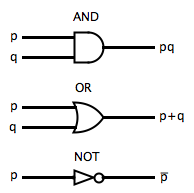
\includegraphics[width=\linewidth,height=!,scale=0.75]{graphics/AndOrNot.png}
%\begin{tikzpicture}[circuit logic US]
%\matrix[column sep=1cm]
%{
%  \node (a0) {$p$}; & \node {\textsc{and}}; & & \\
%  & \node [and gate] (a2) {}; & \node (a3) {$pq$}; & \\
%  \node (a1) {$q$}; & & & \\
%  \node (o0) {$p$}; & \node {\textsc{or}}; & & \\
%  & \node [or gate] (o2) {}; & \node (o3) {$p+q$}; & \\
%  \node (o1) {$q$}; & & & \\
%  & \node {\textsc{not}}; & \\
%  \node (n0) {$p$}; & \node [not gate] (n1) {}; & \node (n2) {$\overline{p}$}; \\
%};
%\draw (a2.input 1) -- ++(left:4mm) |- (a0.east);
%\draw (a2.input 2) -- ++(left:4mm) |- (a1.east);
%\draw (a2.output) -- (a3.west);
%\draw (o2.input 1) -- ++(left:4mm) |- (o0.east);
%\draw (o2.input 2) -- ++(left:4mm) |- (o1.east);
%\draw (o2.output) -- (o3.west);
%\draw (n1.input) -- (n0.east);
%\draw (n1.output) -- (n2.west);
%\end{tikzpicture}
\end{center}

The final result is a circuit diagram such as Figure~\ref{fig:exprcircuit}.
\begin{figure}
\begin{center}
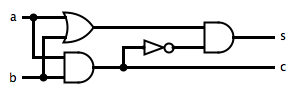
\includegraphics[width=!,height=!,scale=0.75]{graphics/HalfAdder.png}
%\begin{tikzpicture}[circuit logic US]
%\matrix[column sep=1cm]
%{
%  \node [or gate] (o1) {}; & & \node [and gate, yshift=-1mm] (a2) {}; & \node [yshift=-1mm] (s) {$s$}; \\
%  & \node [not gate] (n1) {}; & & \\
%  \node [and gate] (a1) {}; & & & \node (c) {$c$}; \\
%};
%\node (a) at ([xshift=-1.1cm]o1.input 1) {$a$};
%\node (b) at ([xshift=-1cm]a1.input 2) {$b$};
%\draw (a.east) -- (o1.input 1);
%\draw[*-] (b.east) ++(3mm,-0.8mm) |- (o1.input 2);
%\draw[*-] (a.east) ++(5mm,0.8mm) |- (a1.input 1);
%\draw (b.east) -- (a1.input 2);
%\draw (o1.output) -- ++(right:2cm) |- (a2.input 1);
%\draw (a2.output) -- (s.west);
%\draw (a1.output) -- (c.west);
%\draw[*-] (a1.output) ++(5mm,-0.8mm) |- (n1.input);
%\draw (n1.output) -- ++(right:0.5cm) |- (a2.input 2);
%\end{tikzpicture}
\end{center}
\caption{Circuit diagram for $s=(a+b)\overline{ab}$ and $c=ab$}
\label{fig:exprcircuit}
\end{figure}

It is important to realize, though, that this is just another presentation of the logical expressions we started with. Any set of Boolean expressions may be drawn this way, and any circuit where all of the information flows from left to right may be read as a set of expressions.

In addition to visualizing the layout of gates in a digital circuit, a circuit diagram may be used to ``trace'' its operation on particular inputs. For example, Figure~\ref{fig:exprcircuit11} is our example circuit annotated with \0/\1 logic values on each wire, to trace its behavior when both inputs $a$ and $b$ are 1. Since the logic values flow from left to right, the output of each successive gate may be determined from its inputs. By tracing each combination of inputs, we may construct a truth table corresponding to the circuit; the result is
\[ \begin{array}{cc|cc}
a  & b  & c & s\\ \hline
\0 & \0 & \0 & \0\\
\0 & \1 & \0 & \1\\
\1 & \0 & \0 & \1\\
\1 & \1 & \1 & \0
\end{array} \]
\begin{figure}
\begin{center}
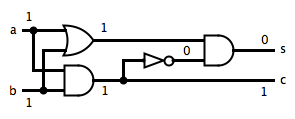
\includegraphics[width=!,height=!,scale=0.75]{graphics/HalfAdder11.png}
\end{center}
\caption{Annotated diagram for $s=(a+b)\overline{ab}$ and $c=ab$ when $a=1$ and $b=1$}
\label{fig:exprcircuit11}
\end{figure}

\paragraph{Implementation of Logic Gates}

It is useful to have some idea of how digital logic gates are built out of lower-level electronic devices such as transistors. For our purposes, a transistor is a voltage-controlled switch: when the voltage is high, the switch is closed (that is, it conducts electricity); when the voltage is low, the switch is open (breaking the connection). Figure~\ref{fig:nmosgates} shows n-type metal-oxide-semiconductor (NMOS) implementations of \textsc{not}, \textsc{nor}, and \textsc{nand} gates; we will study these instead of the more common complementary MOS (CMOS) gates, because they are slightly simpler---CMOS has the practical advantage of using significantly less power, at the cost of doubling the number of transistors, but the basic principles are very similar.

\begin{figure}
\begin{center}
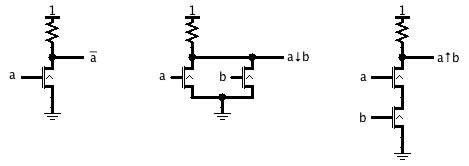
\includegraphics[width=!,height=!,scale=0.75]{graphics/NMOSgates.png}
\end{center}
\caption{NMOS implementations of \textsc{not}, \textsc{nor}, and \textsc{nand} gates}
\label{fig:nmosgates}
\end{figure}

The \textsc{not} gate consists of a single transistor in the lower half: the ``gate'' on the left is connected to the input signal, $a$; the ``source'' at the bottom is connected to ground, and the ``drain'' at the top is connected to the output, $\overline{a}$, and a ``pull-up'' resistor (the jagged line) whose other end is at the high voltage level. When $a=\0$ and the switch is open (so the transistor effectively has infinite resistance), the output will be pulled high (so $\overline{a}=\1$). When $a=\1$ and the switch is closed, the lower resistance through the transistor will pull the output low (so $\overline{a}=\0$).

The \textsc{nor} gate uses two transistors in parallel: if either $a$ or $b$ is high, then the output will be pulled low. Conversely, the \textsc{nand} gate uses two transistors in series: both have to be closed (so $a=b=\1$) for the output to be pulled to \0. Here are the conventional circuit symbols for \textsc{nand} and \textsc{nor} gates (note that the circle on the output indicates negation, just like on the \textsc{not} gate; the unnegated version of \textsc{not}, drawn as a simple triangle, is known as a ``buffer,'' because it copies its input to its output unchanged, after a short delay):
\begin{center}
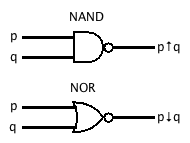
\includegraphics[width=!,height=!,scale=0.75]{graphics/NandNor.png}
\end{center}

Those three gates are the simplest to implement with transistors. As we saw in Section~\ref{ssec:OtherBooleanOps}, all other Boolean operators can be constructed from \textsc{nand} alone, or \textsc{nor} alone. For example, an \textsc{and} gate is a \textsc{nand} followed by a \textsc{not}, so it can be built out of three transistors; an \textsc{or} gate also takes three, using a \textsc{nor} and a \textsc{not}. In the next section, we will see another way to construct circuits using only \textsc{nand} gates.

\begin{tailquote}
Claude Shannon (1916--2001), known as ``the father of information theory,'' wrote his master's thesis at MIT in 1937. Entitled ``A Symbolic Analysis of Relay and Switching Circuits,'' it has been called the most influential master's thesis of the 20\textsuperscript{th} century. In it, he showed how to systematically turn expressions of Boolean algebra into circuits made up of switches.
\end{tailquote}
\begin{exercises}
\problem For each of the following Boolean expressions, draw a corresponding circuit diagram. Try to reuse as many common intermediate results as you can.
\begin{enumerate}
\item $x=\overline{(\overline{a}+b)}+\overline{\overline{b}}+\overline{a}$
\item $x=\overline{\overline{c}a}+\overline{b}$, $y=\overline{\overline{c}b}+\overline{a}$
\item $x=abc+abd+acd+bcd$
\end{enumerate}

\problem For each of the following truth tables, draw a corresponding circuit diagram. \textit{(Hint: First extract one or more Boolean expressions in DNF from the table.)}
\begin{enumerate}
\item \( \begin{array}[t]{cc|cc}
a  & b  & x  & y\\ \hline
\0 & \0 & \0 & \1\\
\0 & \1 & \1 & \0\\
\1 & \0 & \1 & \0\\
\1 & \1 & \0 & \1
\end{array} \)
\item \( \begin{array}[t]{ccc|c}
a  & b  & c  & x\\ \hline
\0 & \0 & \0 & \0\\
\0 & \0 & \1 & \0\\
\0 & \1 & \0 & \0\\
\0 & \1 & \1 & \1\\
\1 & \0 & \0 & \0\\
\1 & \0 & \1 & \1\\
\1 & \1 & \0 & \1\\
\1 & \1 & \1 & \1
\end{array} \)
\end{enumerate}

\problem For each of the following circuit diagrams, write the corresponding Boolean expressions, then trace the output on each combination of inputs and summarize the results in a truth table.
\begin{enumerate}
\item 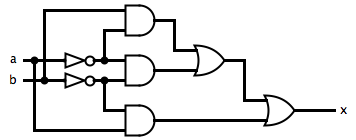
\includegraphics[width=!,height=!,scale=0.75]{graphics/Exercise5213a.png}
\item 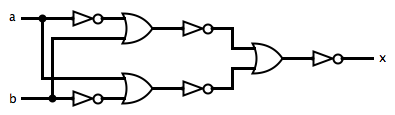
\includegraphics[width=!,height=!,scale=0.75]{graphics/Exercise5213b.png}
\end{enumerate}
\end{exercises}

\subsection{Circuit Simplification}\label{sec:circsimp}
As noted above, a physical circuit does have some dependence on time, since each device in the circuit requires a non-zero time to respond to a change in its inputs. A more precise model needs to take these delays into account---a circuit is modeled by a Boolean expression \emph{plus} a set of delay factors (other cost measures may also be important: power consumption, heat production, area occupied, \textit{etc.}, but we will focus on the delay issue here). We will make the simplifying assumption that all gates have the same delay time, so we will measure the total delay of a circuit in terms of the number of gate delays required before the output values accurately reflect a change to the input values.

Given a combinational circuit, we may compute the delay, also known as the \textit{span}, by finding the number of gates on the longest path (the ``critical path'') from an input to an output. For example, the circuit in Figure~\ref{fig:exprcircuit} has a span of three gate delays, with the critical path going from either $a$ or $b$ to $s$, passing through an \textsc{and}, a \textsc{not}, and another \textsc{and} gate. Note that this is a conservative estimate of the delay required, although for certain inputs the output may become stable sooner---for example, if $a$ and $b$ both change to \0, then after one gate delay the output of the \textsc{or} and the first \textsc{and} will both be \0; that means that in this case, output $c$ will be determined after one gate delay, while output $s$ will be determined after two gate delays (because as soon as one input to the second \textsc{and} is \0, its output will become \0 after one more gate delay regardless of the other input). However, other combinations of inputs may well take the entire three gate delays to correctly determine the value of $s$.

One approach to reducing the delay of a circuit is to use the disjunctive normal form, also known as the ``sum-of-products'' (see Section~\ref{ssec:DNF}). Since an expression in DNF is the \textsc{or} of a collection of terms which are the \textsc{and} of some number of literals, and a literal is either an input or a negated input, the corresponding circuit can be constructed in three layers:
\begin{center}
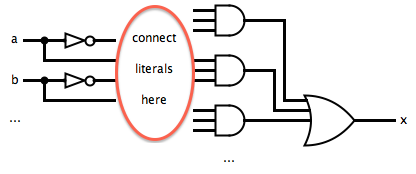
\includegraphics[width=!,height=!,scale=0.75]{graphics/DNFlayers.png}
\end{center}

An interesting property of the sum-of-products representation falls out of the De Morgan laws. Since $ab+cd=\overline{\overline{ab}\cdot\overline{cd}}=(a\uparrow b)\uparrow(c\uparrow d)$, the two layers of \textsc{and} and \textsc{or} gates may be replaced entirely with \textsc{nand} gates to get an equivalent circuit!
\begin{center}
\includegraphics[width=!,height=!,scale=0.75]{graphics/DNFlayersNand.png}
\end{center}

Unfortunately, this does not mean that any Boolean expression can be computed by a circuit with only three gate delays. One problem comes when we need \textsc{and} and \textsc{or} gates (or \textsc{nand} gates) with more than two inputs---in general, with $n$ input variables, there may be \textsc{and} gates that need $n$ literal inputs, and there could be on the order of $2^n$ gates in the \textsc{and} level, requiring an \textsc{or} gate with that many input lines. We will see in the next section how to build gates with a larger number of inputs out of gates with just two inputs.

Another problem with DNF comes if we use the full DNF expression extracted from a truth table. Recall the full DNF expression that we extracted from the truth table for $p\rightarrow q$ in Section~\ref{ssec:OtherBooleanOps}: $\overline{p}\cdot\overline{q}+\overline{p}q+pq$. We were able to use Boolean identities to find an equivalent DNF expression, $\overline{p}+q$ (which only needs two gate delays, since the \textsc{and} layer disappears). There are general techniques for finding simpler DNF expressions such as this; we will look at a simple technique called a \textit{Karnaugh map}, although for computer implementation the related Quine-McCluskey algorithm is better (and for large numbers of input variables a heuristic approach is necessary).

A Karnaugh map is a way of visualizing entries in a truth table so that adjacent entries only differ on the value of one input variable. For example, the entry for $\overline{p}q$ will be next to the entry for $pq$. If adjacent entries each contain 1, meaning that those terms would participate in the full DNF expression, then they may be replaced by a single term with just the variables that are the same: in the example, this corresponds to the simplification $\overline{p}q + pq=(\overline{p}+p)q=1q=q$.

For two input variables, a Karnaugh map is a $2\times 2$ array:
\[ \begin{array}{r|cc}
& \overline{q} & q\\ \hline
\overline{p} & x_{00} & x_{01}\\
p & x_{10} & x_{11}
\end{array} \]
This is just a compact rearrangement of the truth table:
\[ \begin{array}{cc|c}
p & q & x\\ \hline
\0 & \0 & x_{00}\\
\0 & \1 & x_{01}\\
\1 & \0 & x_{10}\\
\1 & \1 & x_{11}
\end{array} \]
However, note that the adjacent cell condition is true: horizontally adjacent cells only differ on $q$, while vertically adjacent cells only differ on $p$.

Once we have laid out the Karnaugh map, a simplified expression may be read off by finding a way to cover all of the 1's in the map with ``implicants.'' An implicant is a rectangle whose side lengths are a power of 2; it corresponds to finding a collection of adjacent cells in the map (all of which contain 1) that all agree on some of the input literals and that collectively include all combinations (negated or not) of the other input variables. The resulting term for an implicant is just the product of the common literals among all the cells covered by the implicant.

On a $2\times 2$ map, the only implicants are individual cells ($1\times 1$), a row ($1\times 2$), a column ($2\times 1$), or the entire map ($2\times 2$). The cells correspond to terms such as $p\overline{q}$, the rows are either $\overline{p}$ or $p$, the columns are either $\overline{q}$ or $q$, and the entire map is $1$ (the empty product). To get the simplest expression, we want to take the fewest number of the largest possible implicants that between them cover all of the 1's in the map. Implicants may overlap, as long as all of (and only) the 1's are covered by at least one implicant.

Here is the example again. First the truth table for $p\rightarrow q$:
\[ \begin{array}{cc|c}
p & q & x\\ \hline
\0 & \0 & \1\\
\0 & \1 & \1\\
\1 & \0 & \0\\
\1 & \1 & \1
\end{array} \]
As a Karnaugh map, this is:
\[ \begin{array}{r|cc}
& \overline{q} & q\\ \hline
\overline{p} & \1 & \1\\
p & \0 & \1
\end{array} \]
The best way to cover this map with implicants is to take the first row and the second column. That gives the simplified terms $\overline{p}$ and $q$, so the final simplified expression is $\overline{p} + q$. Here is the map with the implicants outlined:
\[ \begin{array}{r|cc}
& \overline{q} & q\\ \hline
\overline{p} & \tikzmark{left1}\1 & \tikzmark{left2}\1\tikzmark{right1}\\
p & \0 & \1\tikzmark{right2}
\end{array}
\DrawBox[blue]{left1}{right1}
\DrawBox[red]{left2}{right2} \]

A Karnaugh map can also work with three or four input variables, producing either a $2\times 4$ or a $4\times 4$ array. The same procedure applies, with three complications:
\begin{enumerate}
\item To satisfy the adjacent cell condition, successive rows or columns must change only one variable at a time: for example, the rows might be labelled in order $\overline{p}\cdot\overline{q}$, $\overline{p}q$, $pq$, and $p\overline{q}$;
\item Implicants may be 1, 2, or 4 rows tall by 1, 2, or 4 columns wide; and
\item Implicants may ``wrap around'' from one side of the map to the other.
\end{enumerate}
For example, on a $4\times 4$ map, one possible implicant is the middle two rows; another is the leftmost and rightmost columns (wrapping horizontally); a third is the $2\times 2$ block consisting of the middle two elements of the top row and the middle two elements of the bottom row (wrapping vertically); a final example is the last two elements of the third row. See Figure~\ref{fig:KarnaughImplicants} for these examples.

\begin{figure}
Middle two rows ($q$):
\[ \begin{array}{r|cccc}
& \overline{r}\cdot\overline{s} & \overline{r}s & rs & r\overline{s}\\ \hline
\overline{p}\cdot\overline{q} & & & & \\
\overline{p}q & \tikzmark{left1}1 & 1 & 1 & 1\\
pq & 1 & 1 & 1 & 1\tikzmark{right1}\\
p\overline{q} & & & &
\end{array}
\DrawBox[blue]{left1}{right1} \]

Leftmost and rightmost columns ($\overline{s}$):
\[ \begin{array}{r|cccc}
& \overline{r}\cdot\overline{s} & \overline{r}s & rs & r\overline{s}\\ \hline
\overline{p}\cdot\overline{q} & \tikzmark{left1}1 & & & \tikzmark{left2}1\\
\overline{p}q & 1 & & & 1\\
pq & 1 & & & 1\\
p\overline{q} & 1\tikzmark{right1} & & & 1\tikzmark{right2}
\end{array}
\DrawBoxW[blue]{left1}{right1}
\DrawBoxE[blue]{left2}{right2} \]

Middle elements of top and bottom rows ($\overline{q}s$):
\[ \begin{array}{r|cccc}
& \overline{r}\cdot\overline{s} & \overline{r}s & rs & r\overline{s}\\ \hline
\overline{p}\cdot\overline{q} & & \tikzmark{left1}1 & 1\tikzmark{right1} & \\
\overline{p}q & & & &\\
pq & & & &\\
p\overline{q} & & \tikzmark{left2}1 & 1\tikzmark{right2} &
\end{array}
\DrawBoxN[blue]{left1}{right1}
\DrawBoxS[blue]{left2}{right2} \]

Last two elements of the third row ($pqr$):
\[ \begin{array}{r|cccc}
& \overline{r}\cdot\overline{s} & \overline{r}s & rs & r\overline{s}\\ \hline
\overline{p}\cdot\overline{q} & & & & \\
\overline{p}q & & & &\\
pq & & & \tikzmark{left1}1 & 1\tikzmark{right1}\\
p\overline{q} & & & &
\end{array}
\DrawBox[blue]{left1}{right1} \]
\caption{Some examples of Karnaugh map implicants}
\label{fig:KarnaughImplicants}
\end{figure}

A Karnaugh map also allows us to find simple circuits in the case that some combinations of inputs will never occur, so that we do not care what the output is in those rows of the truth table. By entering a ``don't care'' value, such as X, in the map, we have the freedom to either ignore or include those cells when covering the map with implicants; by including a cell with an X along with a group of 1's, we might be able to construct a larger (and hence simpler) implicant.

For example, suppose we have the following truth table for a four-variable Boolean expression (this represents the inputs that are binary numbers less than ten and divisible by three):
\[ \begin{array}{cccc|c}
p & q & r & s & x\\ \hline
\0 & \0 & \0 & \0 & \1\\
\0 & \0 & \0 & \1 & \0\\
\0 & \0 & \1 & \0 & \0\\
\0 & \0 & \1 & \1 & \1\\
\0 & \1 & \0 & \0 & \0\\
\0 & \1 & \0 & \1 & \0\\
\0 & \1 & \1 & \0 & \1\\
\0 & \1 & \1 & \1 & \0\\
\1 & \0 & \0 & \0 & \0\\
\1 & \0 & \0 & \1 & \1\\
\1 & \0 & \1 & \0 & X\\
\1 & \0 & \1 & \1 & X\\
\1 & \1 & \0 & \0 & X\\
\1 & \1 & \0 & \1 & X\\
\1 & \1 & \1 & \0 & X\\
\1 & \1 & \1 & \1 & X
\end{array} \]
As a Karnaugh map, this is:
\[ \begin{array}{r|cccc}
& \overline{r}\cdot\overline{s} & \overline{r}s & rs & r\overline{s}\\ \hline
\overline{p}\cdot\overline{q} & \1 & \0 & \1 & \0\\
\overline{p}q & \0 & \0 & \0 & \1\\
pq & X & X & X & X\\
p\overline{q} & \0 & \1 & X & X
\end{array} \]
The \1's, plus some of the X's, may be covered by four implicants: $\overline{p}\cdot\overline{q}\cdot\overline{r}\cdot\overline{s}$, $\overline{q}rs$, $qr\overline{s}$, and $ps$. Note that the second implicant wraps around from the third cell on the top row to the third cell (with an X, which is also covered by the $ps$ implicant) on the bottom row; if it were just the \1 on the top row, then the term would be $\overline{p}\cdot\overline{q}rs$, which is not as simple. Here are the cells that end up being covered:
\[ \begin{array}{r|cccc}
& \overline{r}\cdot\overline{s} & \overline{r}s & rs & r\overline{s}\\ \hline
\overline{p}\cdot\overline{q} & \tikzmark{left1}\1\tikzmark{right1} & \0 & \tikzmark{left2a}\1\tikzmark{right2a} & \0\\
\overline{p}q & \0 & \0 & \0 & \tikzmark{left3}\1\\
pq & X & \tikzmark{left4}X & X & X\tikzmark{right3}\\
p\overline{q} & \0 & \1 & \tikzmark{left2b}X\tikzmark{right2b}\tikzmark{right4} & X
\end{array}
\DrawBox[blue]{left1}{right1}
\DrawBoxN[red,rounded corners=3pt]{left2a}{right2a}
\DrawBoxS[red,rounded corners=3pt]{left2b}{right2b}
\DrawBox[green]{left3}{right3}
\DrawBox[purple]{left4}{right4} \]
Therefore, the simplified expression is $\overline{p}\cdot\overline{q}\cdot\overline{r}\cdot\overline{s} + \overline{q}rs + qr\overline{s} + ps$. This may be computed by the following circuit:
\begin{center}
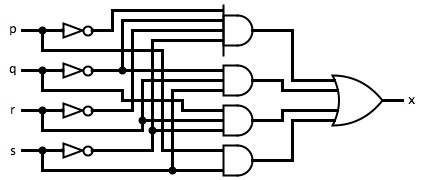
\includegraphics[width=!,height=!,scale=0.75]{graphics/KarnaughExample.png}
\end{center}
In the next section, we will see how to implement this with a total delay of 5, using only two-input \textsc{and} and \textsc{or} gates.

The final difficulty with building low-delay circuits from DNF expressions is that, even with the simplification provided by something like a Karnaugh map, many Boolean functions lead to an exponential blowup when expressed in DNF. In the worst case, an expression with $n$ input variables may require $O(2^n)$ terms in a sum-of-product representation---consider the case of a Karnaugh map where the \1's are in a checkerboard arrangement, so that none are adjacent. When $n$ is large enough, it might not even be practical to consider the truth table at all; for example, a circuit that can add two 32-bit numbers requires 64 input lines, which would lead to a truth table with $2^{64}\approx 10^{19}$ entries. The next section will also discuss approaches to this kind of problem.

\begin{tailquote}
Maurice Karnaugh [pronounced ``CAR-no''] (1924--) developed his map method in 1953, based on a 1952 paper by Edward Veitch (1924--2013), ``A Chart Method for Simplifying Truth Functions.'' The major difference between Karnaugh's and Veitch's diagrams was the ordering of the columns and rows---Veitch put them in straight binary order, while Karnaugh rearranged them to make adjacent cells differ by only one variable. Veitch's approach makes sense if you picture the diagram as showing layers of a cube or hypercube, and arguably extends more readily to five or six variables, but Karnaugh's approach became more popular.
\end{tailquote}

\begin{exercises}
\problem For each of the following Boolean expressions, compute the total delay of the direct translation of the expression into a circuit.
\begin{enumerate}
\item $\overline{(\overline{p}+q)}+(\overline{\overline{q}}+\overline{p})$
\item $(\overline{\overline{r}p}+\overline{q})(\overline{\overline{r}q}+\overline{p})$
\item $(((p+q)(q+r))\,(r+s))\,(((p+r)(q+s))\,(p+s))$
\end{enumerate}

\problem For each of the expressions in the previous problem, use a Karnaugh map to find an equivalent sum-of-products expression, and draw the resulting circuit.

\problem Suppose we want to build a counter that cycles through the numbers 0, 1, 2, 3, 4, and back to 0. One element of this counter will be a circuit that takes the current number, expressed in binary, and outputs the next number. Here is the truth table for this function, with three inputs ($a$, $b$, and $c$) and three outputs ($x$, $y$, and $z$):
\[ \begin{array}{ccc|ccc}
a & b & c & x & y & z\\ \hline
\0 & \0 & \0 & \0 & \0 & \1\\
\0 & \0 & \1 & \0 & \1 & \0\\
\0 & \1 & \0 & \0 & \1 & \1\\
\0 & \1 & \1 & \1 & \0 & \0\\
\1 & \0 & \0 & \0 & \0 & \0\\
\1 & \0 & \1 & X & X & X\\
\1 & \1 & \0 & X & X & X\\
\1 & \1 & \1 & X & X & X\\
\end{array} \]
Since the counter should never reach numbers 5, 6, or 7, we do not care about the output when $abc$ is \1\0\1, \1\1\0, or \1\1\1. Use Karnaugh maps to find a simple circuit for this function.

\problem\label{ex:BCD} In binary-coded decimal (BCD), four bits are used to represent the numbers 0 (\0\0\0\0) through 9 (\1\0\0\1); the other six bit patterns (\1\0\1\0 through \1\1\1\1) are unused. BCD is often used in circuits where decimal numbers need to be displayed; a common device for doing so is the ``seven-segment display.'' Using only seven elements (for example, light-emitting diodes), we may form a reasonable approximation of all the digits 0--9: \textifsym{0123456789}. Construct a truth table with four inputs and seven outputs showing how to produce these characters from input in BCD (be sure to include a diagram indicating which output column corresponds to which display element). Use Karnaugh maps to design a relatively simple circuit that implements a seven-segment decoder.

\problem Exercise~\ref{ex:CNF} of Section~\ref{ssec:DNF} examines conjunctive normal form (CNF), the dual of DNF. Explore what kind of circuits result from CNF, and how to extract a simplified CNF expression from a Karnaugh map \textit{(Hint: look at blocks of \0's.)}.
\end{exercises}

\subsection{Common Circuit Components}
Just as a complicated piece of software is never written from scratch entirely from the most basic program statements, a complicated hardware design is not approached purely at the gate level. Where a programmer will break the task into a hierarchy of objects and functions, relying on familiar idioms and existing code from program libraries to avoid reinventing the wheel, a hardware designer will use a hierarchy of functional blocks, relying on familiar patterns and existing libraries of subcircuits.

We have already seen one of these common components---the sample circuit in Figure~\ref{fig:exprcircuit} is known as the ``half adder.'' If $a$ and $b$ represent one-bit binary numbers, then $s$ is their one-bit sum and $c$ is the carry into the next bit. For example, when $a$ and $b$ are both \1, $s$ is \0 and $c$ is \1; in binary, this says $1+1=10$. We may represent this block in a circuit diagram with an appropriately named box:
\begin{center}
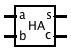
\includegraphics[width=!,height=!,scale=0.75]{graphics/HalfAdderSymbol.png}
\end{center}
It is called a half adder because, when you are adding multiple columns of bits, it only does half the work: it adds the two bits for a column, but it doesn't add in the carry from the next smaller column. A ``full adder'' takes three inputs: $a$ and $b$, plus the incoming carry, $c_\textit{\scriptsize in}$. The outputs are $s$, the sum that stays in the column, plus the outgoing carry to the next column, $c_\textit{\scriptsize out}$. We may build a full adder out of two half adders by first adding $a$ to $b$, then adding $c_\textit{\scriptsize in}$; since the highest total in a full adder is three (\1\1), we will never have a carry out of more than one of the half adders, so the resulting $c_\textit{\scriptsize out}$ is just the \textsc{or} of the two half adder carries. Here is the circuit with its block symbol and its truth table:
\[
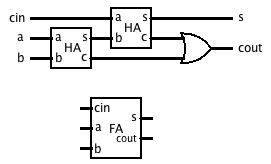
\includegraphics[width=!,height=!,scale=0.75]{graphics/FullAdder.png}\hspace{1cm}
\begin{array}[b]{ccl|rc}
a & b & c_\textit{\scriptsize in} & c_\textit{\scriptsize out} & s\\ \hline
\0 & \0 & \0 & \0 & \0\\
\0 & \0 & \1 & \0 & \1\\
\0 & \1 & \0 & \0 & \1\\
\0 & \1 & \1 & \1 & \0\\
\1 & \0 & \0 & \0 & \1\\
\1 & \0 & \1 & \1 & \0\\
\1 & \1 & \0 & \1 & \0\\
\1 & \1 & \1 & \1 & \1
\end{array}
\]

Given a full adder, we may construct multiple-bit adders by ``cascading'' them, with the carry from each column feeding into the next. Here, for example, is a four-bit adder; the inputs are $a_3a_2a_1a_0$ and $b_3b_2b_1b_0$, plus an incoming carry $c_\textit{\scriptsize in}$ to column 0 (the one's column), and the outputs are $s_3s_2s_1s_0$, plus a carry from column 3 (the eight's column), $c_\textit{\scriptsize out}$:
\begin{center}
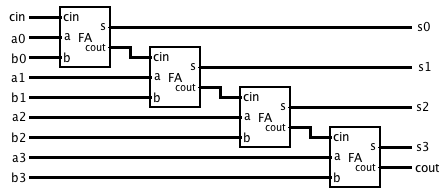
\includegraphics[width=!,height=!,scale=0.75]{graphics/4BitAdder.png}
\end{center}
Exercise~\ref{ex:cascade} explores whether this is a good design.

A common pattern in logic circuits is to use the \textsc{and} gate to ``enable'' (or disable) some signal. For example, in the half adder, the sum output, $s$, is true when one of the inputs is true ($a+b$), except it is disabled when there is a carry (both are true, $a\cdot b$). For another example, suppose we have a circuit which is supposed to compute one of two functions, either $f$ or $g$, depending on a ``select'' input; the circuit might look like this:
\begin{center}
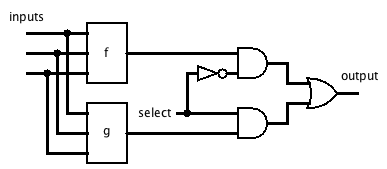
\includegraphics[width=!,height=!,scale=0.75]{graphics/ForG.png}
\end{center}
When \textit{select} is \0, the output is computed by $f$; when it is \1, the output is computed by $g$.

The idea of selecting from two signals may be generalized to using a $k$-bit input to select from one of up to $2^k$ signals; the result is known as a ``multiplexer'' (often abbreviated MUX). For example, with two select lines, $s_1s_0$, you can choose one of four inputs: $a_{00}$, $a_{01}$, $a_{10}$, or $a_{11}$. Each input is enabled by an appropriate combination of the select lines and their complements, then all four possibilities (of which at most one may be true) are combined with \textsc{or}. Here is the circuit and its common symbol:
\begin{center}
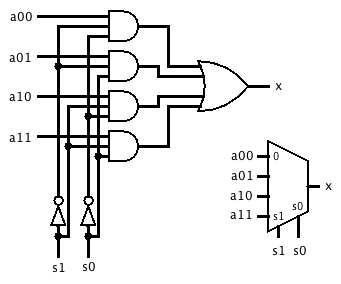
\includegraphics[width=!,height=!,scale=0.75]{graphics/MUX.png}
\end{center}

Note the similarity of the multiplexer circuit to the layers of the sum-of-products circuit from Section~\ref{sec:circsimp}. If we view the input lines $a_{ij}$ as the enabling inputs, then a multiplexer gives a direct way of implementing a truth table: hard-wire the input lines to \0 or \1 according to the corresponding entries in the truth table, then use the select lines to choose the desired row to send to the output. For example, if $a_{01}$ and $a_{10}$ are both tied to \1, while $a_{00}$ and $a_{11}$ are \0, then the output of the multiplexer will be the exclusive-\textsc{or} of $s_1$ and $s_0$.

The opposite of a multiplexer is a ``demultiplexer'' (DEMUX). It takes one input signal plus $k$ select lines, and delivers the input signal to one of $2^k$ output lines. A special case is known as a ``($k$-bit) decoder'': if the input signal is fixed at \1, then the decoder will send a \1 to exactly one of its output lines. Alternately, a demultiplexer can be viewed as a decoder with an ``enable'' input, where the selected output line will be \1 only if the enabling input signal is \1. Here is the common symbol for a four-line demultiplexer:
\begin{center}
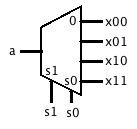
\includegraphics[width=!,height=!,scale=0.75]{graphics/DEMUX.png}
\end{center}
The implementation of this circuit is left as an exercise.

\begin{tailquote}
Edward F.~Moore (1925--2003) described his finite state machine model (see Section~\ref{sec:moore}) in a 1956 paper entitled ``Gedanken-Experiments on Sequential Machines.'' In it, he considered machines as ``black boxes,'' completely determined by their inputs and outputs (as an extreme, he considered ``infernal machines,'' where one possible output is that it explodes\ldots). The combinational circuits in this section are the special case of boxes where there is no state dependence on previous inputs.
\end{tailquote}
\begin{exercises}
\problem\label{ex:cascade} Compute the total gate delays for a half adder, a full adder, and a four-bit cascaded adder as described in this section. The total delay is the maximum number of gate delays between any input signal changing and all output signals stabilizing to reflect the changed input.

\problem Draw the circuit diagram for an implementation of a four-line demultiplexer.

\problem A ``parity bit generator'' is a circuit that takes some number of lines of input and produces one output which is \0 if an even number of the inputs are \1, and \1 if an odd number of the inputs are \1. If the input bits are transmitted along with the generated parity bit, then a recipient can check whether any single bit was mis-transmitted by ensuring that the total number of \1 bits received is even. A two-input parity bit generator is just the exclusive-\textsc{or} circuit, whose common symbol is:
\begin{center}
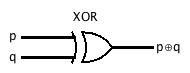
\includegraphics[width=!,height=!,scale=0.75]{graphics/XOR.png}
\end{center}
Give an implementation of a two-input parity bit generator using only \textsc{nand} gates, and then show how to use \textsc{xor} gates to build an eight-input parity bit generator.

\problem The opposite of a decoder is an ``encoder'': given $2^k$ input lines, the output will be a $k$-bit binary number representing which input is \1. In case more than one input line is \1, the output will give the highest such line number; this is known as a ``priority encoder.'' For example, when $k=3$, if lines $a_1$, $a_4$, and $a_5$ are all \1, while the rest are \0, then the output will be \1\0\1 (5 in binary). If no input line is \1, then the output will be \0\0\0. There is one additional output line, $g$ (the ``group'' signal) that will only be \1 if at least one of the inputs is \1; this allows us to tell the difference between no input and only line $a_0$ being \1.

Give a truth table for a four-input ($k=2$) priority encoder, then draw a circuit diagram that implements it.
\end{exercises}

\subsection{Divide-and-Conquer Design}
See Sections~13.5--7 of Aho \& Ullman.
\begin{exercises}
\problem Show how to construct a $2k$-input parity bit generator given a block that implements a $k$-input parity bit generator.

\problem Show how to construct a $2k$-input priority encoder given a block that implements a $k$-input priority encoder.
\end{exercises}




% !TEX root = main.tex

\section{Sequential Circuits}
All of the circuits we have considered so far have been acyclic; this was an essential part of the definition of a combinational circuit. In general, if a circuit has a cycle, its output behavior might not be well-behaved---consider the simple example of a \textsc{not} gate whose output feeds back to its input, so that if the output went high, it would be forced low after one gate delay, then back high after another delay, \textit{etc}.\footnote{In fact, since a physical device can only be an approximation of a pure logic gate, it is more likely that the output would hover around some intermediate level, neither high nor low.}

In this section, we will explore two ways of adding cycles to circuits in a controlled fashion. The first, operating on the level of just a few gates, will give us circuit components with memory. The second, using larger-scale feedback on circuits that include both combinational and memory components, will give us a means of implementing state machines and, ultimately, general-purpose processors. On the larger scale, the circuits will be what are known as ``synchronous''---that is, a clock signal is used to synchronize the times at which feedback is applied. At the small scale, we will start with ``asynchronous'' circuits, where feedback may arrive as soon as the gate delays permit. While it is possible to design large-scale asynchronous circuits, we will not be considering that here.

Circuits with cycles are known as ``sequential logic'' circuits, because the output depends on the particular \emph{sequence} of inputs the device has received in the past; unlike combinational circuits, the output is not solely determined by the current combination of input values but potentially by the entire history of inputs (in other words, it is not purely functional---its behavior depends on side-effects). As a result, they can be considerably harder to reason about, and we will need good abstract models, such as state machines.

\subsection{Memory Devices}
Although the circuit with one \textsc{not} gate feeding back on itself is unstable, a cycle of two \textsc{not} gates would be fine:
\begin{center}
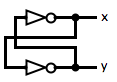
\includegraphics[width=!,height=!,scale=0.75]{graphics/NotLatch.png}
\end{center}
Whatever the output is at $x$, the output at $y$ will be the opposite. Each one feeds back and reinforces the other, and the circuit is stable. Unfortunately, it is not very useful---there is no way to provide input to \emph{change} the value $x$.

By replacing the \textsc{not} gates with either \textsc{nand} or \textsc{nor} gates, we get a circuit known as a latch. Here is the diagram for a so-called $\overline{SR}$ latch:
\begin{center}
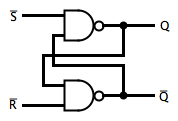
\includegraphics[width=!,height=!,scale=0.75]{graphics/SRLatch.png}
\end{center}
When the inputs $\overline{S}$ (set) and $\overline{R}$ (reset) are both \1, the latch behaves just like the circuit with two \textsc{not} gates (because $\1\uparrow x=\overline{x}$): whatever the output is at $Q$, the opposite value will be at $\overline{Q}$ (hence its customary label---it is the negation of $Q$).

When the $\overline{S}$ input is \0, the output $Q$ is forced to \1---the latch is ``set'' (the label $\overline{S}$ suggests that it is ``active-low'': the latch will be set when the input is false). Again, because of the feedback, when $Q$ is \1, $\overline{Q}$ will be \0. Returning $\overline{S}$ to \1 \emph{will then leave the latch in the set state}. This is where the sequential nature of the latch shows: its state depends on its past history (in this case, the fact that the set line was most recently active).

When the $\overline{R}$ input is \0, the output $\overline{Q}$ is forced to \1 and correspondingly $Q$ will become \0---the latch has been ``reset.'' Again, returning $\overline{R}$ to \1 will leave it in the reset state, until the set line is next activated.

If both the set and reset lines are active (\0), then both output lines will be forced to \1. This presents two problems: it violates the property that $Q$ and $\overline{Q}$ are complementary, and it sets up a potential race condition if both lines are restored to \1 at the same time. When the inputs are \1, exactly one of the outputs can be high; however, which one ``wins'' the race will depend on the precise timing of the transitions from \0 to \1, and potentially also on slight imperfections in the gates (if one of the \textsc{nand} gates responds slightly faster than the other, for example). So, don't do that.

The $\overline{SR}$ latch is what is known as a \textit{transparent} latch: the output responds as soon as the input is changed. To make sequential design easier, we frequently want memory devices that will only respond at certain times. By adding an extra layer of gates to the input, we can make what is known as a ``gated D latch.'' The inputs are $D$ (data) and $E$ (enable):
\begin{center}
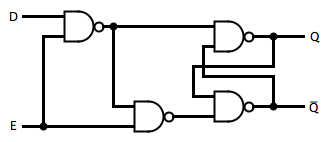
\includegraphics[width=!,height=!,scale=0.75]{graphics/DELatch.png}
\end{center}
As long as $E$ is \0 (note that this is now an active-high device), the $\overline{S}$ and $\overline{R}$ inputs to the latch will always be \1, regardless of the $D$ input. The gated D latch is only enabled when the $E$ input is \1. When enabled, the latch becomes transparent: if $D$ is \1, then $\overline{S}$ will be \0, and the output $Q$ will be set to \1; if $D$ goes to \0, then $\overline{R}$ will be \0 and the latch will be reset. There is no combination of inputs for $D$ and $E$ which can make both the set and reset lines active at the same time, so we don't have to worry about that case.

When the enable line returns to \0, the gated D latch will remain in whatever state it last entered. Here is a truth table for the latch, together with its common symbol when used in a circuit:
\[ \begin{array}[b]{cc|cc}
E & D & Q & \overline{Q}\\ \hline
\0 & X & \multicolumn{2}{c}{\textrm{last state}}\\
\1 & \0 & \0 & \1\\
\1 & \1 & \1 & \0
\end{array}\hspace{1cm}
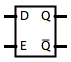
\includegraphics[width=!,height=!,scale=0.75]{graphics/DELatchSymbol.png}
\]

When dealing with a sequential circuit, it is often helpful to look at a \emph{timing diagram}, which shows the levels at various points of the circuit over time (increasing from left to right). Here is a timing diagram for the gated D latch, which shows that the output is transparent to the $D$ input only when $E$ is high:
\[ \begin{array}{cc}
E & \texttiming{2C2C2C2C}\\
D & \texttiming{LHLHLHLH}\\
Q & \texttiming{LLLHHHLH}
\end{array} \]

Instead of a latch, it is more common to use a device known as a ``flip-flop.'' The distinction from a latch is that a flip-flop will only respond to input for a very brief time; it is what is known as a \textit{clocked} device, since it will only change its state when a clock pulse is received (typically, just as the clock pulse is rising from \0 to \1). In \emph{synchronous} logic design, the entire circuit will use a single clock signal, so that each clock pulse advances the state by one step (and the state has time to propagate through all the gate delays before the next pulse). Here is one design for an edge-triggered D flip-flop:
\begin{center}
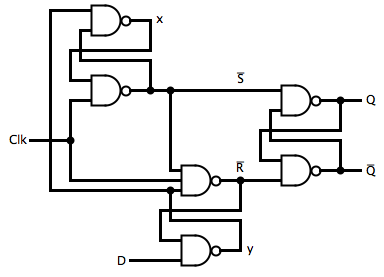
\includegraphics[width=!,height=!,scale=0.75]{graphics/DFlipFlop.png}
\end{center}
Just as the gated D latch modified an $\overline{SR}$ latch by adding a layer of two \textsc{nand} gates, this flip-flop modifies an $\overline{SR}$ latch by adding a layer of two input latches. In each case, the input layer protects the output latch from entering the illegal state (both $\overline{S}$ and $\overline{R}$ low).

The idea is that, as long as the clock (\textit{Clk}) is \0, the set ($\overline{S}$) and reset ($\overline{R}$) lines of the output latch will stay high (inactive). The line marked $x$ will be whatever $D$ is, and the line marked $y$ will be the opposite, $\overline{D}$. Although one of the input latches will be in an ``illegal'' state, the output latch will not be affected.

When the clock goes to \1, the input latches will resolve to consistent states: $\overline{S}$ will be $\overline{x}=\overline{D}$, and $\overline{R}$ will be $\overline{y}=D$. That is, if $D$ was \0, then the output latch will be reset, while if $D$ was \1 it will be set. However, once the clock reaches \1, further changes to $D$ will be ignored: if the lower input latch is reset ($\overline{R}$ is \0, meaning $D$ was \0 at the rising edge), then changing $D$ will leave it in the reset state; if instead the lower input latch is set ($\overline{R}$ is \1, meaning $D$ was \1 at the rising edge), then changing $D$ will switch it between the set and illegal states (where $\overline{R}$ is still \1), and the upper input latch will stay in the set state.

When the clock goes back to \0, the output latch will continue to hold whatever state it had (because both of its inputs will be \1 again), until the next time the clock rises.

The only danger with this design is if $D$ is changed at exactly the same time as the rising of the clock signal, because then if one of the input latches was in an illegal state it is possible to have a race condition. Designers avoid this by arranging for the $D$ input to be stable for at least a brief ``setup and hold'' time around clock pulses.

Here is a timing diagram for the D flip-flop, and its common circuit signal (the input marked with a triangle indicates that it is a rising-edge-triggered clock):
\[ \begin{array}[b]{rc}
\textit{Clk} & \texttiming{2C2C2C2C2C2C2C2C}\\
D & \texttiming{lLHLHLLLHHHLHLHHh}\\
Q & \texttiming{LLHHHHLLLLHHHHHH}
\end{array}\hspace{1cm}
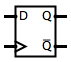
\includegraphics[width=!,height=!,scale=0.75]{graphics/DFlipFlopSymbol.png}
\]

Rather than a truth table, it is useful to give what are known as a \emph{characteristic table} or an \emph{excitation table} for a flip-flop. The characteristic table shows how the input ($D$) and current state ($Q$) lead to the next state ($Q'$) after the clock pulse:
\[ \begin{array}{cc|c}
D & Q & Q'\\ \hline
\0 & \0 & \0\\
\0 & \1 & \0\\
\1 & \0 & \1\\
\1 & \1 & \1
\end{array} \]
The excitation table presents the same information, but from the viewpoint of ``given a current state $Q$ and desired next state $Q'$, what does the input need to be?''
\[ \begin{array}{cc|c}
Q & Q' & D\\ \hline
\0 & \0 & \0\\
\0 & \1 & \1\\
\1 & \0 & \0\\
\1 & \1 & \1
\end{array} \]

\begin{tailquote}
The first electronic latch was the Eccles-Jordan trigger circuit. Patented in 1918, it was built out of two vacuum tubes connected in a feedback loop. In the early 1940's, Thomas Flowers (1905--1998) used his experience with telephone switching circuits to build Colossus, one of the code-breaking machines at Bletchley Park. The Colossus design used the Eccles-Jordan circuit as a storage register; it is considered the first programmable, electronic, digital computer, although its existence was kept secret until the 1970's.
\end{tailquote}
\begin{exercises}
\problem Investigate the behavior of a latch built with \textsc{nor} gates instead of the \textsc{nand} gates used in the $\overline{SR}$ latch. Use this new latch to build a gated D latch.

\problem There are several other types of flip-flops besides the D. Perhaps the most general is the JK flip-flop, which has two inputs, traditionally named $J$ and $K$, along with a clock input and the complementary $Q$ and $\overline{Q}$ outputs. When $J$ and $K$ are both \0 and a clock pulse arrives, the state does not change. When only $J$ is \1, the new state will be \1; when only $K$ is \1, the new state will be \0 (so $J$ \emph{sets} and $K$ \emph{resets} the flip-flop). Finally, when both $J$ and $K$ are \1, the clock pulse will cause the state to \emph{toggle}---that is, it will switch to the negation of its previous state. Here is the characteristic table of the JK flip-flop, using $X$ to indicate ``don't care'' inputs:
\[ \begin{array}{ccc|c}
J & K & Q & Q'\\ \hline
\0 & \0 & \0 & \0\\
\0 & \0 & \1 & \1\\
\0 & \1 & X & \0\\
\1 & \0 & X & \1\\
\1 & \1 & \0 & \1\\
\1 & \1 & \1 & \0
\end{array} \]
\begin{enumerate}
\item Draw a timing diagram that shows the behavior of the JK flip-flop.
\item Give an excitation table for the JK flip-flop.
\item Show how to construct a JK flip-flop using a D flip-flop plus a few extra gates. \textit{(Hint: Combine the $J$ and $K$ inputs with the current outputs $Q$ and $\overline{Q}$ to generate an appropriate $D$ input.)}
\end{enumerate}

\problem Random-access memory (RAM) devices can be made from a quantity of flip-flops plus a few extra components such as multiplexers and demultiplexers. To store $2^k$ individually-addressable bits, you need one D type flip-flop per bit. The $D$ inputs can all be connected to an incoming data line; if each flip-flop's clock signal is driven by one line of a $k$-bit demultiplexer whose input signal is the \textsc{and} of the system clock signal and a ``write enable'' input, then the flip-flop selected by the $k$ address lines will be loaded with the desired data only if a write is enabled at the rise of the clock. Connecting the outputs of the flip-flops to a multiplexer, whose $k$ select lines are also driven by the $k$-bit address, will cause the contents of the selected bit to be passed to the output of the MUX. Use this description to draw a 16-bit RAM circuit, then show how to expand it to store four bits at each address.
\end{exercises}

\subsection{State Machines}
In Section~\ref{sec:moore} we learned about Moore machines, a version of finite state automata where there is an output associated with each state. Using flip-flops, we can build a circuit that implements a Moore machine. Here is a block diagram for such a circuit (although the connections are shown as single wires, all but the clock may be several bits wide):
\begin{center}
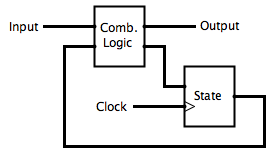
\includegraphics[width=!,height=!,scale=0.75]{graphics/MooreMachine.png}
\end{center}
In addition to the feedback within each flip-flop, there is a larger-scale feedback loop of the current state back to provide input for the next step. The box labelled ``Comb. Logic'' is a combinational circuit with two functions: compute an output based on the current state, and compute the next-state control signals based on the input and the current state. The box labelled ``State'' is one or more flip-flops; when a clock pulse arrives, it takes the control signals from the combinational logic and advances to the next state---the \emph{state} of the machine is simply the current states of these flip-flops.

If there are $k$ flip-flops, each of which can be \0 or \1, then the machine can be in $2^k$ different states. Therefore, if our Moore machine needs $n$ states, we will need at least $\lceil\lg n\rceil$ flip-flops. One step in designing the circuit for a given machine will be to assign a binary encoding to each state. For example, if the machine has three states, $A$, $B$, and $C$, then we will need two flip-flops. The circuit state will be the combination of the flip-flop outputs: $Q_1Q_0$. Given this, we may arbitrarily choose the encoding $A=\0\0$, $B=\0\1$, and $C=\1\0$ (and the state $\1\1$ will go unused).

Although the diagram shows the combinational logic has both the machine input and the current state available to compute the output, the convention in a Moore machine is that only the state is used to determine the output. There is a practical reason for this: during a clock cycle, as soon as the current state has propagated through the logic gates, we want the output to be available and stable. The input signals may not be stable until close to the end of the cycle (just before they are needed to determine the next state), and we would prefer not to see ``glitches'' in the output while the input might still be changing.

Here is an example of this process. Consider the following state machine for a mod-3 up/down counter:
\begin{center}
\begin{tikzpicture}[->,>=stealth',shorten >=1pt,auto,node distance=2.8cm,semithick]
  \node[initial,state](q0){$q_0/\0\0$};
  \node[state](q1)[right of=q0]{$q_1/\0\1$};
  \node[state](q2)[right of=q1]{$q_2/\1\0$};
  
  \path(q0) edge             node {\0} (q1)
            edge [bend left] node {\1} (q2)
       (q1) edge             node {\0} (q2)
            edge [bend left] node {\1} (q0)
       (q2) edge [bend left,in=120,out=60] node {\0} (q0)
            edge [bend left] node {\1} (q1);
\end{tikzpicture}
\end{center}
It has one input; call it $a$. When $a$ is \0, each clock pulse increments the counter through the states $q_0$, $q_1$, $q_2$, and back to $q_0$. When $a$ is \1, it decrements. At each state, the output is the corresponding number in binary: \0\0, \0\1, and \1\0.

We will use two D flip-flops, and the obvious encoding of states to bit patterns (which also happens to be the mapping from state to output, so we can just use the current state, \0\0, \0\1, or \1\0, to drive the output directly). All that remains is to design the combinational circuit that computes the $D_1$ and $D_0$ flip-flop control signals based on the input and current state. For this, we will first fill in a truth table with current state, input, and desired next state values, then use the excitation table for the flip-flops to decide an appropriate signal (for type-D flip-flops, this is particularly easy, since the required $D$ input is just the next state $Q'$):
\[ \begin{array}{ccc|cc|cc}
\multicolumn{2}{c}{\textit{current}} & \textit{input} &
  \multicolumn{2}{c}{\textit{next}} & \multicolumn{2}{c}{\textit{control}}\\
Q_1 & Q_0 & a & Q_1' & Q_0' & D_1 & D_0\\ \hline
\0 & \0 & \0 & \0 & \1 & \0 & \1\\
\0 & \0 & \1 & \1 & \0 & \1 & \0\\
\0 & \1 & \0 & \1 & \0 & \1 & \0\\
\0 & \1 & \1 & \0 & \0 & \0 & \0\\
\1 & \0 & \0 & \0 & \0 & \0 & \0\\
\1 & \0 & \1 & \0 & \1 & \0 & \1
\end{array} \]
Here is the Karnaugh map for $D_1$:
\[ \begin{array}{r|cccc}
& \overline{Q}_1\overline{Q}_0 & \overline{Q}_1Q_0 & Q_1Q_0 & Q_1\overline{Q}_0\\ \hline
\overline{a} & \0 & \tikzmark{left2}\1 & X\tikzmark{right2} & \0\\
a & \tikzmark{left1}\1\tikzmark{right1} & \0 & X & \0
\end{array}
\DrawBox[blue]{left1}{right1}
\DrawBox[red]{left2}{right2} \]
And here is the map for $D_0$:
\[ \begin{array}{r|cccc}
& \overline{Q}_1\overline{Q}_0 & \overline{Q}_1Q_0 & Q_1Q_0 & Q_1\overline{Q}_0\\ \hline
\overline{a} & \tikzmark{left1}\1\tikzmark{right1} & \0 & X & \0\\
a & \0 & \0 & \tikzmark{left2}X & \1\tikzmark{right2}
\end{array}
\DrawBox[blue]{left1}{right1}
\DrawBox[red]{left2}{right2} \]
Therefore, simple DNF expressions for the control signals are $D_1=\overline{Q}_1\overline{Q}_0a+Q_0\overline{a}$ and $D_0=\overline{Q}_1\overline{Q}_0\overline{a}+Q_1a$. The full circuit for the counter is given in Figure~\ref{fig:Mod3Counter}.
\begin{figure}
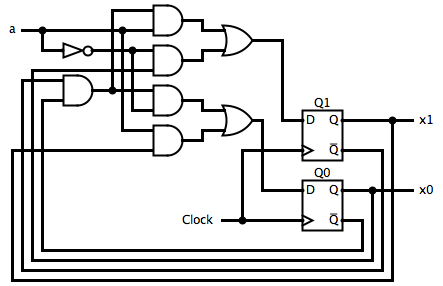
\includegraphics[width=!,height=!,scale=0.75]{graphics/Mod3Counter.png}
\caption{State machine circuit for a mod-3 up/down counter}
\label{fig:Mod3Counter}
\end{figure}

\begin{tailquote}
With combinational circuits to perform arithmetic and logic operations on data, plus registers to store intermediate results and keep track of program steps, a sequential circuit allows us to model an entire central processing unit. By connecting the inputs and outputs to external storage and I/O devices, the CPU forms the core of a general-purpose computer; details are left to the reader.
\end{tailquote}
\begin{exercises}
\problem Design a BCD accumulator whose input is a three-bit two's complement number representing the value to be added to the total. That is, the state will be a decimal digit 0--9, represented in binary (\0\0\0\0 through \1\0\0\1). The output should be the signal lines to drive a seven-segment display (see Exercise~\ref{ex:BCD} of Section~\ref{sec:circsimp}). If the input is \0\0\0, then the state will be unchanged. If the input is +1 (\0\0\1) through +3 (\0\1\1), then that number will be added on each clock pulse. If the input is -4 (\1\0\0) through -1 (\1\1\1), then the total will go down by that amount on each pulse.

\problem Reinterpret the block diagram for a Moore machine to produce a Mealy machine, where an output is associated with each transition. That is, the output should be determined by the current state \emph{and} the input. What might happen to the output if the input changes during a clock cycle? Compare this behavior to a Moore machine.
\end{exercises}



% !TEX root = main.tex

\chapter{Functional Programming}
% !TEX root = main.tex

\section{Introduction to Scala}
\startchapter{The Scala programming language} is a relative of Java that enables what is known as a ``functional'' programming style; what this means will be the subject of much of the rest of this chapter. This introduction assumes that you are already familiar with programming in Java and/or C++. You may not be an expert, but you are comfortable with writing classes and methods. We will by no means be learning all of Scala here, and when there are multiple ways to express something in Scala we will generally just choose one. The emphasis is on becoming able to read and write simple functions to manipulate the kinds of data models talked about in the Foundations class: lists, trees, graphs, \textit{etc}. Although Scala also has extensive support for an object-oriented style of programming, we will be focusing on its support for functional programming.

Before diving into the details, here is a short sales pitch for Scala. This is a quote from the main Scala website, \url{http://www.scala-lang.org/}:
\begin{quotation}
Scala\index{Scala} is a general purpose programming language designed to express common programming patterns in a concise, elegant, and type-safe way. Scala smoothly integrates features of object-oriented and functional languages, enabling developers to be more productive while retaining full interoperability with Java and taking advantage of modern multicore hardware.
\end{quotation}
Scala is a real-world, commercial-strength language, being used at companies such as Twitter, LinkedIn, Verizon, and many others; one of its attractions to these businesses is that it is very compatible with existing Java code, while also supporting more advanced programming techniques as found in functional languages such as Haskell and F$^\sharp$, or in dynamic languages such as Python and Ruby.

The ``functional'' programming style referred to above is not meant to imply that other styles are dysfunctional; rather, it refers to an emphasis on building programs out of pure functions. A pure function\index{pure function}\index{function!pure} is a block of code whose result depends only on the values of its input parameters; just like a function in mathematics, every time it is called with the same arguments it will return the same result. Furthermore, calling a pure function must have no side-effects\index{side-effect}---it will not change the state of any external variable, nor perform input or output, nor throw an exception.

Clearly we do not want to write entire programs with no side-effects, since they could never interact with the user. However, the functional style\index{functional style} encourages a program structure where all external effects are handled at the outermost layer, with the main body of the program composed entirely out of pure functions. There are many advantages to this design: functional code is easier to reason about and to test, it is more likely to be reusable, and it may well be easier to optimize for different hardware configurations, such as multicore processors or distributed clusters.

One consequence of performing a computation in a pure function is that it has a property known as ``referential transparency.''\index{referential transparency} The essence of this is that a function call may be replaced by its result value at any point in a program without affecting the behavior of the program (except perhaps its running time). This enables us to reason about functional programs using a substitution model,\index{substitution model} just as used in algebra: if we know that the referentially transparent expressions $e_1$ and $e_2$ are equal, then whenever we see $e_1$ in a program we may replace it with $e_2$.

Here is an example of a Java function that is \emph{not} pure:\index{function!impure}
\begin{verbatim}
public int double(int n) {
  System.out.println("Doubling " + n);
  runningTotal += n;
  return 2 * n;
}
\end{verbatim}
Each time \verb|double(n)| is called, it has two side-effects:\index{side-effect} it prints a message to the console and it modifies an external variable (\verb|runningTotal|, which is presumably an instance variable or static field of a containing class). Now consider the following program fragment:
\begin{verbatim}
int x = double(3) * double(3)
\end{verbatim}
The resulting value of \verb|x| will be 36, but the net effect of executing that statement in Java will be different from either of the following:
\begin{verbatim}
int y = double(3);
int x = y * y;
\end{verbatim}
or
\begin{verbatim}
int x = 6 * 6;
\end{verbatim}
When we deal with impure functions, our ability to reason about and manipulate code becomes significantly more complicated than just performing substitution.

In Scala, a pure function definition will have the following form:\index{Scala!function definition}
\begin{verbatim}
def <function-name>(<parameters>): <type> = <expression>
\end{verbatim}
The parameters\index{Scala!parameters} should be a comma-separated list of zero or more entries of the form \verb|<variable-name>: <type>|. Variable and function names\index{Scala!identifiers} follow the usual rules for Java identifiers (with some extensions we will see later): they must start with a letter, and consist of letters, digits, or underscores. The expression on the right-hand side should have the given return type;\index{Scala!return type}\footnote{In many cases Scala can infer\index{type inference} the return type if it is not provided, but we will see an important case where it cannot, so it is a good habit to always specify it.} it may be a simple expression or a block surrounded by braces.\index{Scala!block} If it is a block, then all but the last statement should be definitions of local functions or constants;\footnote{We will see later that blocks may also contain local import statements and definitions of objects, classes, traits, or types. Statements before the end of the block can also be expressions, but since they could only be evaluated for their side-effects,\index{side-effect} we will not need this in functional code.} the last statement will be the expression whose value is returned. A constant definition\index{Scala!constant definition} has the form:
\begin{verbatim}
val <variable-name> = <expression>
\end{verbatim}
An explicit type may be given after the name, such as \verb|val n: Int = 42|, but Scala is usually able to infer the correct type without this.

For example, here is a function that returns the square of the double of its integer argument (there are simpler ways to do this, but we want to explore the possibilities):
\begin{verbatim}
def squareDouble(k: Int): Int = {
  def double(n: Int): Int = 2 * n
  val x = double(k)
  x * x
}
\end{verbatim}
Note that, in addition to the placement of the type annotation \emph{after} the variable, Scala has another minor syntactic difference from Java: semicolons are optional at the end of a line.

As an example of reasoning by substitution,\index{substitution model} here is one way to evaluate a function call such as \verb|squareDouble(3)|:
\[ \begin{array}{rcl}
\verb|squareDouble(3)| & = & \verb|x * x|,\quad
\begin{array}[t]{l}
\textit{where }\verb|x = double(3)|\\
\textit{and }\verb|double(n) = 2 * n|
\end{array}\\
& = & \verb|x * x|,\quad
\begin{array}[t]{l}
\textit{where }\verb|x = 2 * 3|
\end{array}\\
& = & \verb|x * x|,\quad
\begin{array}[t]{l}
\textit{where }\verb|x = 6|
\end{array}\\
& = & \verb|6 * 6|\\
& = & \verb|36|
\end{array} \]

We will occasionally have need of modifiable local variables,\index{Scala!variable definition} which are defined like constants but use the keyword \verb|var| instead of \verb|val|. A variable may be assigned\index{Scala!assignment} a new value after definition with an assignment statement, just as in Java:
\begin{verbatim}
var x = 1
x = x + 1  // after this, x will be 2
\end{verbatim}
However, this reduces the purity of the code (reasoning about an expression containing \verb|x| needs to take into account what its current value is, whether it is before or after an assignment), and in general we will prefer ``immutable''\index{immutability} variables (\textit{i.e.}, constants). When we deal with larger data structures, this preference for immutability will continue.

\begin{tailquote}
In 1977, John Backus\index{Backus, John} (1924--2007)---one of the inventors of the Fortran programming language---was awarded the highest prize in computing, the Turing Award. The lecture he gave at the award ceremony was titled ``Can Programming Be Liberated from the von Neumann Style? A Functional Style and Its Algebra of Programs.'' Backus enumerated many of the problems he had seen with languages such as Fortran, and his algebraic approach to reasoning about pure expression-based programs influenced much subsequent research in functional programming.
\end{tailquote}
\begin{exercises}
\problem Consider the following Scala function:
\begin{verbatim}
def exercise(a: Int, b: Int): Int = {
  def m(x: Int, y: Int): Int = x - y
  def s(n: Int): Int = n * n
  val c = m(a, b)
  val d = m(a, c)
  val e = c + d
  s(d) - s(e)
}
\end{verbatim}
\begin{enumerate}
\item What is the value of \verb|exercise(4, 5)|?
\item What is the value of \verb|exercise(12, 13)|?
\item Use algebraic substitution to evaluate \verb|exercise(a, b)| in terms of the variables \verb|a| and \verb|b|.
\end{enumerate}

\problem Write a Scala function named \verb|average| that takes three integer arguments and calculates their average. For example, \verb|average(7, 1, 2)| should return \verb|3| (use integer division, which rounds toward zero).

\problem Write a Scala function named \verb|median| that takes three integer arguments and calculates their median (that is, the middle of the three numbers when they are put in increasing order). For example, \verb|median(7, 1, 2)| should return \verb|2|. You may use the library functions \verb|math.min(a, b)| and \verb|math.max(a, b)|, which respectively return the smaller and the larger of their arguments.
\end{exercises}

\section{Types}
While it is not strictly necessary to have explicit types\index{types} for a language to be functional, it is important to have a notion (perhaps only in the programmer's mind) of the range of values allowed for a given variable or expression, as well as the ways it may be used (for example, whether it may be applied to an argument). Scala has a rich set of mechanisms for describing types, and the compiler will check that the explicitly declared types in a program are consistent.

In this and following sections, we will walk through a useful subset of these types, and describe the corresponding code constructs for operating on them. One recurrent theme will be that the type of the data determines the structure of the program; once you know the input and output types of a function, you can often lay out a skeleton for how the function must be written.

\paragraph{Booleans}
The simplest type conveying a non-trivial amount of information is the common \verb|Boolean| type,\index{types!Boolean} whose values may only be \verb|true| or \verb|false|. Scala has the usual relational operators\index{Scala!relational operators}\index{operators!relational} (\verb|==|, \verb|!=|, \verb|<=|, \textit{etc}.) familiar from Java and other C-derived languages; the only difference here is that the equality test defaults to checking equality of values, rather than just object identity (so you do not have to remember to use \verb|.equals| on strings\ldots). It also has the familiar logical operators\index{Scala!logical operators}\index{operators!logical} \verb|&&| (\textsc{and}), \verb-||- (\textsc{or}), and \verb|!| (\textsc{not}).

The obvious way to use a Boolean value is with an \verb|if| expression\index{Scala!if expression}:
\begin{verbatim}
if (<test>) <true-clause> else <false-clause>
\end{verbatim}
If the expression \verb|<test>| evaluates to \verb|true|, then the whole expression evaluates to \verb|<true-clause>|, otherwise it evaluates to \verb|<false-clause>|. Note that, in Scala, \verb|if| is an \emph{expression} rather than a statement---it may be used anywhere a value is needed that depends on the result of a test. For example, here is an absolute value function:
\begin{verbatim}
def absoluteValue(x: Double): Double = if (x >= 0) x else -x
\end{verbatim}

Another running theme in Scala is the use of ``pattern matching''\index{Scala!match expression}\index{pattern matching} to take values apart. For a Boolean value, the appropriate pattern match takes the following form:
\begin{verbatim}
<test> match {
  case true => <true-clause>
  case false => <false-clause>
}
\end{verbatim}
The behavior in this case is exactly the same as the above \verb|if| expression; performing this operation on Booleans is so common that the shorter \verb|if| form is generally used.

\paragraph{Primitives}
Scala is usually compiled to run on the same virtual machine as Java (although there are other alternatives), so it is not surprising that it offers the same range of primitive types\index{types!primitive} as Java. Just about the only difference is that the type names are capitalized: integers are \verb|Int|, floating-point numbers are \verb|Double|, and characters are \verb|Char|. We will stick to these primitive types in this book, although the others (such as \verb|Long|, \verb|Byte|, and \verb|Float|) are also available.\footnote{The intuition for primitive values is that they can be stored in a small, fixed number of bytes and operated on by single machine instructions.}

All of the usual literal constants\index{Scala!literals} and operators are carried over from Java, except the ``cast'' operation is not directly supported. If you want to convert a \verb|Double| to an \verb|Int|, for example, use the \verb|toInt| method:\footnote{Note that, unlike Java, Scala treats even primitive values as if they were objects with methods.} \verb|x.toInt| instead of \verb|(int) x|.

One interesting generalization in Scala is that all operators\index{Scala!operators}\index{operators!Scala} are treated as method calls. For example, \verb|a + b| is compiled as if it were \verb|a.+(b)|. This allows us to extend the available operators by defining our own methods with ``symbolic'' names. In fact, operators don't need to be symbols---any single-argument method may be used as an operator. Thus, the \verb|max| method on numbers, where \verb|a.max(b)| is the larger of \verb|a| and \verb|b|, may also be written as \verb|a max b|.

Pattern matching\index{pattern matching} on primitives looks like the usual \verb|switch|/\verb|case| statement from C and Java, except as above it produces an expression whose value is given by the matching case:
\begin{verbatim}
def factorial(n: Int): Int = n match {
  case 0 => 1
  case _ => n * factorial(n - 1)
}
\end{verbatim}
The second case in this example uses the ``wildcard'' pattern,\index{wildcard}\index{_@\_} \verb|_| (underscore). This pattern matches anything, so it serves as the \emph{default} case. This example also demonstrates defining a function recursively,\index{function!recursive} where the value at one argument depends on first computing the value for some other argument; we will have much more to say about this below.\footnote{Defining a recursive function is the situation mentioned above where the compiler is not always able to infer a return type;\index{Scala!return type}\index{type inference} in the example, it would have to know that \texttt{factorial} returns an \texttt{Int} before it could figure out the type on the right-hand side.}

Patterns may also have ``guard''\index{Scala!guard expression} expressions---tests that have to evaluate to \verb|true| for the case to match. For example, here is a match that converts a character representing a hexadecimal digit to its integer value; if the digit is invalid, it returns \verb|-1|:
\begin{verbatim}
digit match {
  case d if '0' <= d && d <= '9' => d - '0'
  case d if 'A' <= d && d <= 'F' => d - 'A' + 10
  case d if 'a' <= d && d <= 'f' => d - 'a' + 10
  case _ => -1
}
\end{verbatim}

\paragraph{Strings}
A Scala string\index{types!string}\index{Scala!strings} is literally the same as a Java string, at least when compiled to the Java VM. Some additional methods have been added for convenience, such as:
\begin{itemize}
\item \verb|head|, which returns the first character (\verb|s.head| is the same as \verb|s.charAt(0)|),
\item \verb|tail|, which returns all but the first character (\verb|s.tail| is the same as \verb|s.substring(1, s.length())|), and
\item \verb|toInt|, which attempts to parse an integer value from its string representation (\verb|s.toInt| is the same as \verb|Integer.parseInt(s)|).
\end{itemize}
Note that these methods, which are defined in terms of some underlying Java methods, are not strictly pure\index{function!impure}---in each case, they may throw an exception if the string doesn't satisfy some precondition (for \verb|head| and \verb|tail|, it must be non-empty; for \verb|toInt|, it must consist only of one or more digits, optionally preceded by a sign \verb|+| or \verb|-|). However, Java strings (unlike strings in C or C++) \emph{are} immutable, so at least no operation on a string can change the underlying character sequence.\index{immutability}

As mentioned above, strings may be compared for equality with the \verb|==| operator. They have also been extended with comparison operators,\index{Scala!relational operators}\index{operators!relational} so \verb|s < t| is true when \verb|s| lexically precedes \verb|t|.

A convenient extension in Scala is the ability to specify strings that contain special characters, such as quotes and newlines, by enclosing them in triple quotes (these are called ``raw strings''):\index{Scala!raw strings}
\begin{verbatim}
"""This is a string with several lines.
This is the second line, which contains a quotation: "Hello World".
This is the third line."""
\end{verbatim}
To make this easier when code is indented, there is a method named \verb|stripMargin| that will remove leading characters up to the first vertical bar on each line:
\begin{verbatim}
"""This is a string with several lines.
  |This is the second line, which contains a quotation: "Hello World".
  |This is the third line.""".stripMargin
\end{verbatim}

Another extension to the notation for strings is ``string interpolation.''\index{Scala!string interpolation}\index{$@\$} This is actually a very general and extensible facility in the language, but in its simplest form, if you prefix a string literal with the letter \verb|s|, then any occurrence of \verb|$|$x$ in the string will be replaced by the value of variable $x$ (converted to a string, if necessary). Instead of a single variable, an entire expression \textit{expr} may be interpolated if it is enclosed in braces: \verb|${|\textit{expr}\verb|}|. Here is an example:
\begin{verbatim}
s"The value of x is $x, and x*7 is ${x*7}."
\end{verbatim}
If $x$ is 6, then this evaluates to \verb|"The value of x is 6, and x*7 is 42."|

Pattern matching on strings is similar to that on primitives: each case specifies a string literal to be matched, or a guard expression to be satisfied.\index{pattern matching} Later in the book, when we see regular expressions, there will be a more general notion of pattern matching for strings.

\paragraph{Tuples}
If a function needs to return more than one value, it is convenient to be able to package up several values into a single object. In Java, you might create a new class with the desired fields (think of the \verb|Point| class, with \verb|x| and \verb|y| fields). In Scala, a simpler option is to create a ``tuple''\index{types!tuple} (sometimes called an $n$-tuple,\index{n-tuple@$n$-tuple} where $n$ is the number of values). A tuple value is written by giving a comma-separated list of values in parentheses; for example, \verb|(42, "Hello World", false)|. The corresponding type is written as a list of types in parentheses; for example, \verb|(Int, String, Boolean)|.

A 2-tuple is also known as a pair\index{pair} (and a 3-tuple is a triple, \textit{etc.}). An interesting special case is the 0-tuple: the only value is the empty tuple, \verb|()|. The type of the empty tuple is \verb|Unit|;\index{types!unit} it plays the same role as \verb|void| in Java. A function that takes a \verb|Unit| argument might as well not take an argument, because the single value provides no information. A function that \emph{returns} the \verb|Unit| type is suspicious: if it doesn't return a value, then the only reason to call it must be to perform some side-effect.\index{side-effect} Indeed, one of the places we will encounter the \verb|Unit| type is as the return value of non-pure functions\index{function!impure} such as \verb|println|.

Individual elements of a tuple may be accessed with the methods \verb|_1|,\index{_1@\texttt{\_1}} \verb|_2|,\index{_1@\texttt{\_2}} \textit{etc.} However, it is often more natural to extract elements of a tuple with pattern matching.\index{pattern matching} For example, the \verb|splitAt| method on strings returns a pair of strings: \verb|s.splitAt(n)| yields \verb|(a, b)|, where \verb|a.length == n| and \verb|a + b == s|. We may extract these two strings from the pair\index{pair} as follows:
\begin{verbatim}
s.splitAt(n) match {
  case (first, second) =>
    s"""The first $n characters are "$first",
       |and the rest are "$second".""".stripMargin
}
\end{verbatim}
If \verb|s| is \verb|"Hello World"| and \verb|n| is 5, then the result of this expression is
\begin{verbatim}
The first 5 characters are "Hello",
and the rest are " World".
\end{verbatim}

Patterns may be combined, such as a tuple pattern containing literal or wildcard patterns. For example, here is one way to define a Boolean \textsc{and} function:
\begin{verbatim}
def and(x: Boolean, y: Boolean): Boolean = (x, y) match {
  case (false, _) => false
  case (_, false) => false
  case _ => true
}
\end{verbatim}
These cases say that if either \verb|x| or \verb|y| is \verb|false|, then the result is \verb|false|; otherwise it is \verb|true|. Note that the first two cases overlap: if \verb|x| and \verb|y| are both false, then both patterns will match. Scala always chooses the first case with a matching pattern (so a default case, if present, must occur last). Also notice the technique of combining \verb|x| and \verb|y| into a tuple so that the pattern match can depend on both.\index{pattern matching}

\begin{tailquote}
In programming, a type system serves to prevent certain kinds of errors when a program is run. Types\index{types} were used in the early 20\textsuperscript{th} century for a similar purpose: they prevented certain paradoxes when formalizing mathematical logic. This is not entirely coincidental---many aspects of computer hardware and programming languages were influenced by the work of logicians such as Alan Turing,\index{Turing, Alan} Alonzo Church,\index{Church, Alonzo} and Haskell Curry.\index{Curry, Haskell}
\end{tailquote}
\begin{exercises}
\problem Consider this Scala function:
\begin{verbatim}
def foo(m: Int, n: Int): Int = n match {
  case 0 => 1
  case _ if n % 2 == 1 => m * foo(m, n - 1)
  case _ =>
    val p = foo(m, n / 2)
    p * p
}
\end{verbatim}
Recall that \verb|%| is the mod operator: \verb|a % b| is the remainder when \verb|a| is divided by \verb|b|.\index
\begin{enumerate}
\item What is the value of \verb|foo(3, 0)|?
\item What is the value of \verb|foo(3, 1)|?
\item What is the value of \verb|foo(3, 2)|?
\item What is the value of \verb|foo(3, 3)|?
\item What is the value of \verb|foo(3, n)|, in terms of \verb|n|?
\end{enumerate}

\problem Write Scala functions that compute the inclusive and exclusive \textsc{or} operations. That is, write Boolean functions \verb|or(x, y)| and \verb|xor(x, y)| that will return \verb|true| if one of \verb|x| or \verb|y| is \verb|true|; in the inclusive case, \verb|or(true, true)| is also \verb|true|, while for the exclusive case, \verb|xor(true, true)| is \verb|false|. Use pattern matching for one, and \verb|if| expressions for the other (but do not use the built-in logical operators such as \verb-||-).

\problem Define a function \verb|minmax(a: Int, b: Int)| that returns a pair of numbers, where the first is the smaller of \texttt{a} and \texttt{b}, and the second is the larger. For example, \verb|minmax(17, 42)| and \verb|minmax(42, 17)| should both return the pair \verb|(17, 42)|.

\problem Using the \texttt{minmax} function, define a function \verb|sort3(a: Int, b: Int, c: Int)| that returns a triple of numbers which are \texttt{a}, \texttt{b}, and \texttt{c} in non-decreasing order. For example, \verb|sort3(3, 1, 4)| should return the triple \verb|(1, 3, 4)|. \textit{Hint:} Use \texttt{minmax} to find the correct order of \texttt{a} and \texttt{b}, then use it two more times to place \texttt{c} in the correct relative position among variables \texttt{small}, \texttt{middle}, and \texttt{large}, then simply return the triple \verb|(small, middle, large)|.

\end{exercises}

\section{Collection Types}
The Scala standard library provides quite a few types of collections,\index{types!collection} similar to those in the Java standard library but with a more functional treatment. Here are details on a few of them; see the online Scala documentation at \url{http://www.scala-lang.org/api/current/}\index{Scala!documentation} for more.
\begin{itemize}
\item \textbf{Lists}:\index{types!list}\index{Scala!lists} If $x_0$, $x_1$, $x_2$, \ldots\ are values all of the same type $T$, then \texttt{List($x_0$, $x_1$, $x_2$, \ldots)} has type \texttt{List[$T$]} (this is akin to the Java parameterized type \texttt{List<$T$>}). Another name for the empty list is \texttt{Nil}, and values may be added to the front of a list using the \texttt{::}\index{::@\texttt{::}} operator,\footnote{Operators ending with a colon are ``right-associative''\index{Scala!right-associative operators}\index{operators!right-associative} in Scala, so this is the same as \texttt{1 ::\ (2 ::\ (3 ::\ Nil))}, which turns into the chain of method calls \texttt{Nil.::(3).::(2).::(1)}.} so \verb|1 :: 2 :: 3 :: Nil| is an equivalent way of constructing \texttt{List(1, 2, 3)}, of type \texttt{List[Int]}. Given two lists, they may be appended with the \texttt{:::}\index{:::@\texttt{:::}} operator: \verb|List(1, 2) ::: List(3, 4)| produces \verb|List(1, 2, 3, 4)|.

The front element of a (non-empty) list $a$ may be retrieved using the \texttt{head} operation: \texttt{$a$.head}; the list of everything except the head is \texttt{$a$.tail}. For example, \texttt{List(1, 2, 3).head} is \texttt{1}, while \texttt{List(1, 2, 3).tail} is \texttt{List(2, 3)}. It is often better to decompose a list with pattern matching:\index{pattern matching}
\begin{verbatim}
myList match {
  case Nil => println("The list is empty")
  case h :: t => println(s"The head is $h and the tail is $t")
}
\end{verbatim}
Since every list is either empty (\texttt{Nil}) or the concatenation of a head element onto a tail list, \texttt{myList} will match one of the two cases. In the second case, the names \texttt{h} and \texttt{t} (which may be arbitrary variable names) will be bound to the corresponding parts of the list. This is an instance of pattern matching over ``case classes,''\index{Scala!case classes} which are described more below.

Here is another example for lists:
\begin{verbatim}
val front = myList match {
  case Nil => sys.error("Empty list")
  case f :: _ => f
}
\end{verbatim}
If \texttt{myList} is empty, then the \texttt{sys.error} function will throw an exception with the given message; otherwise, the first element will be bound to \texttt{f} (which is a newly created variable, local to the match), then returned as the result of the match, and ultimately assigned to \texttt{front}.

\item \textbf{Vectors}:\index{types!vector}\index{Scala!vectors} If $x_0$, $x_1$, $x_2$, \ldots\ are values of some type $T$, then \texttt{Vector($x_0$, $x_1$, $x_2$, \ldots)} has type \texttt{Vector[$T$]} (this is akin to the Java type $T$\verb|[]|, although the contents are immutable;\index{immutability} see below). Just as with Java and C++ arrays, vectors are zero-indexed. Element $i$ of vector $v$ is named by the expression \texttt{$v$($i$)}, so if \texttt{$v$.size} is $n$, then the elements of $v$ are \texttt{$v$($0$)} through \texttt{$v$($n-1$)}. Note that indexing\index{Scala!indexing} into a vector looks just like a function call (that is, Scala uses parentheses instead of the  square-bracket notation common to C, C++, and Java); this is intentional, since a vector can be thought of as a function over the domain $\{0, 1, \ldots, n-1\}$. To create a vector containing $n$ copies of some value $x$, use \texttt{Vector.fill($n$)($x$)}. To create a vector corresponding to some function $f$ over the domain $\{0, 1, \ldots, n-1\}$, use \texttt{Vector.tabulate($n$)($f$)}---in the resulting vector of size $n$, element $0$ will be $f(0)$, \textit{etc}.

As mentioned above, vectors are immutable. Scala also contains mutable versions of most of its collections; the mutable vector type is named \verb|Array|,\index{types!array} and all of the above operations are available.

\item \textbf{Sets}:\index{types!set}\index{Scala!sets} The type \texttt{Set[$T$]} is very similar to \texttt{List[$T$]}, except that, just like a mathematical set, it does not keep track of the order in which the elements were inserted, and it does not keep duplicate elements. That is, \texttt{Set(1, 2, 3)} is the same as \texttt{Set(3, 1, 1, 3, 2)}. The fundamental operation on a set is to check whether it contains a particular value: \texttt{$a$.contains($x$)} returns \texttt{true} if $x$ is an element of $a$.\footnote{A set may also be used as a function in Scala: \texttt{$a$($x$)} is the same as \texttt{$a$.contains($x$)}.}

\item \textbf{Maps}:\index{types!map}\index{Scala!maps} A common data structure in dynamic languages is the ``associative array,''\index{associative array} which behaves like an array with indices more general than the integers 0 to $n-1$. For example, it is often useful to be able to index into a collection using a string: after setting \texttt{age("George")}\index{Howard, George} to \texttt{17}, we may retrieve George's age by supplying the index \texttt{"George"} to the map \texttt{age}. The Scala type \texttt{Map[$K$, $T$]} provides this facility: if $k_0$, $k_1$, $k_2$, \ldots\ are \emph{keys} of type $K$, and $x_0$, $x_1$, $x_2$, \ldots\ are values of type $T$, then \texttt{Map($k_0$ -> $x_0$, $k_1$ -> $x_1$, $k_2$ -> $x_2$, \ldots)} will map each key to its corresponding value. If \texttt{age} is \texttt{Map("Alice" -> 9, "Susanna" -> 14, "George" -> 17)},\index{Howard, Alice}\index{Howard, Susanna} then \texttt{age("George")} will be \texttt{17}, as desired; the type of \texttt{age} is \texttt{Map[String, Int]}.

By the way, the expression \texttt{"Alice" -> 9} is another way to write the pair\index{pair}\index{->@\texttt{->}} \texttt{("Alice", 9)}. A map is essentially a set of pairs, stored in a data structure that makes it efficient to use the map as a function to look up the value corresponding to a key. Given a map $m$, the expression \texttt{$m$.keySet} produces a set containing all of the keys for which the map is defined; in the example, \texttt{age.keySet} will be the same as \texttt{Set("George", "Susanna", "Alice")} (remember that order does not matter in a set).

\item \textbf{Options}:\index{types!option}\index{Scala!options} A common source of errors in Java is the convention of returning \texttt{null}\index{null} to indicate that some object was unavailable (for example, given a Java map similar to the \texttt{age} example above, \texttt{age.get("Fred")} would return \texttt{null}). Scala attempts to avoid this by providing the ``option'' type: a value of type \texttt{Option[$T$]} is either \texttt{Some($x$)}, where $x$ is a value of type $T$, or it is the special value \texttt{None}. The advantage over returning \texttt{null} is that \texttt{None} is an actual object; attempting to call a method on it will not result in a null pointer exception. The option type is also a signal to the programmer to be prepared for the case of a non-existent object; in Java, it is too easy to ignore this possibility because \emph{every} object type allows \texttt{null}. To retrieve the contained value from an option object, use the \texttt{get} method: \texttt{Some($x$).get} yields $x$. Attempting to call \texttt{get} on \texttt{None} will throw an exception, so a useful variant is the \texttt{getOrElse} method: \texttt{$a$.getOrElse($y$)} will return the contents of $a$, if any, or $y$ if $a$ was \texttt{None}.

Just as with tuples and lists, it is often better style to use pattern matching on options.\index{pattern matching} For example, if \texttt{a} is of type \texttt{Option[T]}, then
\begin{verbatim}
a match {
  case Some(t) => t
  case None => y
}
\end{verbatim}
will have the same effect as \texttt{a.getOrElse(y)}.

\end{itemize}

\begin{tailquote}
As in many languages, the collections are one of the most important parts of Scala's standard library. Over the years, they have gone through several designs, attempting to maximize their flexibility and efficiency while remaining easy to use. As this is being written, another redesign effort is in progress\ldots.
\end{tailquote}
\begin{exercises}
\problem Evaluate the following expressions and explain what operations are being performed:
\begin{enumerate}
\item \verb|List(3, 1, 4) ::: List(2, 3, 5)|
\item \verb|Set(3, 1, 4) & Set(2, 3, 5)|
\item \verb-Set(3, 1, 4) | Set(2, 3, 5)-
\item \verb|Set(3, 1, 4) &~ Set(2, 3, 5)|
\item \verb|Set(3, 1, 4).subsets.toSet|
\end{enumerate}

\problem For each of the following expressions, predict what the result will be, then check your prediction by evaluating it in Scala:
\begin{enumerate}
\item \verb|Map(1 -> 1, 2 -> 4, 3 -> 9)(2)|
\item \verb|Map(1 -> 1, 2 -> 4, 3 -> 9)(4)|
\item \verb|Map(1 -> 1, 2 -> 4, 3 -> 9).get(4)|
\item \verb|Map(1 -> 1, 2 -> 4, 3 -> 9) get 2|
\item \verb|Map(1 -> 1, 2 -> 4, 3 -> 9).keySet|
\end{enumerate}

\problem Write and test a \texttt{match} expression that takes a pair of integer lists and returns the smaller of the head elements. If only one list is non-empty, return its head; if both are empty, signal an error with a call to \texttt{sys.error}. For testing purposes, you will need to use \verb|List[Int]()| to enter an empty list. Thus, you should see the following results:
\begin{itemize}
\item \verb|(List(1, 2), List(3, 4, 5)) match ...| produces \texttt{1};
\item \verb|(List(1, 2), List(0, -1, 2)) match ...| produces \texttt{0};
\item \verb|(List(1, 2), List[Int]()) match ...| produces \texttt{1};
\item \verb|(List[Int](), List(3, 4, 5)) match ...| produces \texttt{3};
\item \verb|(List[Int](), List[Int]()) match ...| produces an error.
\end{itemize} 
\end{exercises}

\section{Control Structures}
As with expressions, the control structures\index{Scala!control structures} such as \texttt{if}\index{Scala!if expression} and \texttt{while}\index{Scala!while loop} are substantially the same in Scala as in Java and C++. For example, the following code fragment works exactly the same in all three languages (assuming that \verb|n| has been declared as a \verb|var|):
\begin{verbatim}
while (n != 1) {
  if (n % 2 == 0) {
    // n is even
    n = n / 2;
  } else {
    // n is odd
    n = 3 * n + 1;
  }
}
\end{verbatim}
One minor difference already noted is that Scala doesn't require the semicolons at the end of each simple statement, although they are allowed. A more significant innovation is that statements and control structures all produce values, so they may be used in expressions. The \texttt{while} loop only produces the value \texttt{()} of type \texttt{Unit}, so that isn't particularly useful. However, as we have seen, the \texttt{if} statement evaluates to one of its two branches, depending on the test, so the above code may also be written
\begin{verbatim}
while (n != 1) {
  n = if (n % 2 == 0) n / 2
      else 3 * n + 1
}
\end{verbatim}

In a block of code\index{Scala!block} surrounded by braces, the value produced is the value of the final expression. For example,
\begin{verbatim}
x = {
  while (j != 0) {
    val temp = j
    j = i % j
    i = temp
  }
  i
}
\end{verbatim}
The value eventually assigned to \texttt{x} is the final value of \texttt{i}, after some number of times through the loop (in fact, this code assigns the GCD of \texttt{i} and \texttt{j} to \texttt{x}). There \emph{is} a \texttt{return} statement\index{Scala!return statement} in Scala, which breaks out of a block and returns a value from the enclosing function, but it is generally used only when the normal program flow must be altered, preventing control from reaching the end of the block.

Scala does \emph{not} provide the same \texttt{for} loop as its predecessors. Part of the reason for this is that it discourages writing code that relies on modifying, or ``mutating,''\index{immutability} values bound to variables (Scala doesn't even provide the operator \texttt{++}, which is found so frequently in counting-based \texttt{for} loops, although it does support the shortcut assignment operators\index{operators!shortcut assignment} such as \texttt{+=}). More importantly, though, Scala provides a very nice generalization of the \texttt{for} loop,\index{Scala!for loop} which can iterate through many of the collection types in a uniform way. Given a collection $a$ (other than a tuple), the statement \texttt{for \{$x$ <- $a$\} $b$} will execute the body $b$ once for each value $x$ taken from $a$. The expression \texttt{$x$ <- $a$} is called a ``generator.''\index{generator} For example,
\begin{verbatim}
for {n <- List(3, 1, 4, 1, 5)} {
  println(n)
}
\end{verbatim}
produces the output
\begin{verbatim}
3
1
4
1
5
\end{verbatim}
The typical C++ or Java counting loop, written as \texttt{for (i = 0; i < N; i++)}, becomes \texttt{for \{i <- 0 until N\}}. The expression \texttt{0 until N} produces a ``range''\index{range} collection, which is a sequence where the successive values differ only by a step value; by saying \texttt{until}, the range excludes the final value, \texttt{N}; inclusive ranges are possible with the \texttt{to} operator: \texttt{1 to 3} is the sequence 1, 2, 3. The \texttt{by} operator can be used to get a step other than 1: \texttt{10 to 1 by -1} is the range that counts from 10 down to 1. The value returned from this form of the \texttt{for} loop is \texttt{()}, just as with \texttt{while}.

The \verb|while| loop expects its test to \emph{not} be referentially transparent\index{referential transparency}---if it always returned the same value then the loop would not work---so it is decidedly not a functional construct. The \verb|for| loop above (often called the ``\verb|for|-each'' loop) is also non-functional, because the loop body must perform some side-effect\index{side-effect} (such as output) for each element in the collection.

A purely functional generalization of the \texttt{for} loop, sometimes called a ``\texttt{for} comprehension,''\index{Scala!for comprehension}\index{for comprehension} can be used to construct a new collection: the expression \texttt{for \{$x$ <- $a$\} yield $b$} evaluates the expression $b$ for each element $x$ in $a$, and gathers all of the results in a collection of the same kind as $a$. For example,
\begin{verbatim}
for {i <- List(3, 1, 4, 1, 5)} yield i * i
\end{verbatim}
produces the result \texttt{List(9, 1, 16, 1, 25)}.

\begin{tailquote}
Although the \verb|while| and \verb|for|-each loops are not functional, the \verb|for| comprehension\index{for comprehension} that produces a new collection has a long history in functional programming, going back to the set-builder construct in the SETL language of the late 1960's (inspired by the corresponding notation from mathematics). More recently, several functional languages, including Scala, have extended the comprehension idea to work on a wide range of types, not just collections, that are known as ``monads.''\index{monad}
\end{tailquote}
\begin{exercises}
\problem Write and test a loop to print the squares of the numbers from \texttt{1} to \texttt{10}:
\begin{center}
\texttt{1 4 9 16 25 36 49 64 81 100}
\end{center}
Write it first as a \texttt{while} loop (you will need to declare a loop variable with a statement such as \verb|var i = 1|), then write it as a \texttt{for} loop. The \texttt{print} function outputs a string without advancing to the next line.

\problem Do the same exercise as above, but use nested loops to print a $3\times 3$ multiplication table:
\begin{center}
\texttt{1 2 3}\\
\texttt{2 4 6}\\
\texttt{3 6 9}
\end{center}

\problem The generalized \texttt{for} loop has a number of additional features. For example, nested loops\index{Scala!nested loop} may be combined into a single loop with a list of generators:
\begin{verbatim}
for {
  i <- Set(1, 2, 3)
  j <- Set('a', 'b', 'c')
} yield (i, j)
\end{verbatim}
There is actually a subtle difference between this and the nested version:
\begin{verbatim}
for {i <- Set(1, 2, 3)} yield
  for {j <- Set('a', 'b', 'c')} yield (i, j)
\end{verbatim}
Try each, identify the difference, and explain which one is more useful for performing a common operation on sets.
\end{exercises}

\section{Classes}
As a means to encapsulate related fields and methods, Scala's classes\index{Scala!classes}\index{types!class} are quite similar to Java's. Perhaps the most significant difference is in the form of the constructor:\index{Scala!constructor} where Java declares a method with the same name as the class, Scala merges the constructor body with the class definition itself. This, together with other features of the language, frequently leads to a significant reduction in ``boilerplate''\index{boilerplate} code (that is, code which follows a standard, predictable pattern, and which contains very little new information). Here is an example:
\begin{verbatim}
// THIS IS JAVA
public class Triangle {
  private double base;
  private double height;
  private double hypotenuse;

  public Triangle(double base, double height) {
    this.base = base;
    this.height = height;
    this.hypotenuse = Math.sqrt(base * base + height * height);
  }

  public double getBase() {
    return base;
  }

  public double getHeight() {
    return height;
  }

  public double getHypotenuse() {
    return hypotenuse;
  }
}
\end{verbatim}
In Scala, this would typically be written as follows:
\begin{verbatim}
class Triangle(val base: Double, val height: Double) {
  val hypotenuse = math.sqrt(base * base + height * height)
}
\end{verbatim}
The class definition\index{Scala!class definition} header includes the constructor parameters \texttt{base} and \texttt{height}; by making them \texttt{val}s, they will be retained and exposed as read-only fields of the object. The declarations in the body of the object are evaluated with the actual arguments bound to these parameters, so when the field \texttt{hypotenuse} is declared, it will be initialized with the appropriate value. Finally, because we have declared three \texttt{val} fields, there is no need for the getter methods which are so common in Java code; since a \texttt{val} is immutable,\index{immutability} we do not have to worry about other code changing these fields and it is safe to make them public (which is the default in Scala).

An instance of the \texttt{Triangle} class is created just as in Java: \texttt{val t = new Triangle(3.0, 4.0)} instantiates the class with the given constructor arguments, producing a \texttt{Triangle} object. Accessing \texttt{t.hypotenuse} results in \texttt{5.0} (and \texttt{t.base} is \texttt{3.0}, \textit{etc}.).

One aspect of a Scala class that is significantly different from Java is the notion of a static member.\index{static member} In Java, static members are shared among all instances of the class. Scala does not use this concept; instead, it has the notion of a ``companion object.''\index{Scala!companion object} First of all, Scala supports the definition of ``one-off'' objects---singletons,\index{singleton} which are the only instance of their class. An example of this is the \texttt{math} object, which we may imagine being defined as follows:
\begin{verbatim}
object math {
  def max(a: Double, b: Double): Double = if (a > b) a else b
  def sqrt(x: Double): Double = ...
  ...
}
\end{verbatim}
This directly declares an object with the given methods; there is no need to instantiate it, because there will never be more than the one \texttt{math} object. In Java, this corresponds to the \texttt{Math} class having only static members, which are called through the class name (\texttt{Math.sqrt}) rather than through an instance. For this use, the object may be thought of as a ``module''\index{module}---a package of related definitions grouped under an enclosing name. If the bindings in a module are used frequently in a section of code, they may be imported with a statement such as \texttt{import math.\_}.\index{Scala!import statement}\index{_@\_}\footnote{In Java, this is equivalent to writing \texttt{import static Math.*} at the top of a file, although Scala also allows imports that are local to an individual block\index{Scala!block} of code.}

Now suppose we want to have a class of objects with a shared static member. A common example of this is a ``factory''\index{factory method} method: a method that hides the details of constructing an object (perhaps because the actual object returned will belong to a subclass\index{subclass} that the client might not know about). In our \texttt{Triangle} class, suppose the Java version had the following method:
\begin{verbatim}
// THIS IS JAVA
public static Triangle makeIsoceles(double base) {
  return new Triangle(base, base);
}
\end{verbatim}
In Scala, we would put this method in the ``companion''\index{Scala!companion object} of the \texttt{Triangle} class, which is an object also named \texttt{Triangle}:
\begin{verbatim}
object Triangle {
  def makeIsoceles(base: Double): Triangle = new Triangle(base, base)
}
\end{verbatim}
In both cases, we may call \texttt{Triangle.makeIsoceles(1.0)} to produce a new triangle with base and height both 1; the advantage in Scala is that there is a cleaner separation between the operations supported by the entire class and the operations supported by an \emph{instance} of the class.\footnote{Note that there is no ambiguity in naming both the class and its companion \texttt{Triangle}. If \texttt{t} is an object of class \texttt{Triangle}, then \texttt{t.f} is a call to a class (instance) method named \texttt{f}, while a (shared) method \texttt{g} of the companion object must be called as \texttt{Triangle.g}.}

As a hybrid functional/object-oriented language, Scala has equivalents for all of Java's object-oriented features: encapsulation of methods and fields, inheritance, interfaces,  subclass polymorphism, \textit{etc}.\index{object-oriented style} We will not need much from these mechanisms, but here is an example of a class hierarchy with two subclasses:\index{subclass}
\begin{verbatim}
trait Shape {
  def area: Double
  val name: String
  override def toString: String = s"a $name with area $area"
}

class Rectangle(val width: Double, val height: Double) extends Shape {
  def area: Double = width * height
  val name: String = "Rectangle"
}

class Circle(val radius: Double) extends Shape {
  def area: Double = math.Pi * radius * radius
  val name: String = "Circle"
}
\end{verbatim}
A Scala trait\index{Scala!traits} is like an interface in Java, specifying a list of members that will be common to all of its subclasses. They may either be left ``abstract,''\index{abstract member} with no definition bound to the name in the trait, or they may have a (default) definition that will be inherited\index{inheritance} by subclasses unless they choose to override\index{override} it.\footnote{Before Java 8, interfaces were only allowed to contain abstract members, but Java has slowly been adopting some of the features of Scala.} In the example, \texttt{area} and \texttt{name} are abstract, while \texttt{toString} provides a definition (which coincidentally overrides the default definition of the \texttt{toString} method inherited from the base class \texttt{Any}---the keyword \texttt{override} is required when a default behavior is replaced).

The \texttt{Rectangle} and \texttt{Circle} classes extend\index{Scala!extends}\footnote{Scala uses the keyword \texttt{extends} here to mean the same thing as the \texttt{implements} keyword in Java; there is less of a distinction in Scala between ``extending'' a class and ``implementing'' an interface, so the concepts were combined in a single keyword.} the \texttt{Shape} trait, so they may be used in any context where a \texttt{Shape} is expected. For example,
\begin{verbatim}
def expand(shape: Shape): String =
  s"doubling $shape will have area ${4 * shape.area}"
\end{verbatim}
Here is a transcript of calling this function:
\begin{verbatim}
scala> val r = new Rectangle(6, 7)
r: Rectangle = a Rectangle with area 42.0

scala> expand(r)
res1: String = doubling a Rectangle with area 42.0 will have area 168.0
\end{verbatim}

\begin{tailquote}
The language Simula 67, developed in the mid-1960's by Ole-Johan Dahl\index{Dahl, Ole-Johan} (1931--2002) and Kristen Nygaard\index{Nygaard, Kristen} (1926--2002), introduced the concept of classes and subclasses.\index{subclass} The conception was that a class would collect the common properties of several subclasses of objects, to be used as a sort of ``prefix'' to the definition of each subclass.\end{tailquote}
\begin{exercises}
\problem Define a class \texttt{Person} with fields \texttt{givenName}, \texttt{familyName}, and \texttt{birthYear}. Define a computed \texttt{fullName} field that contains a string in the form \verb|"Howard, Brian"| (family name first), and define a method \verb|age(year: Int)| that returns the person's age on their birthday in the given year. Try to make this class definition as short as you can, taking advantage of Scala's boilerplate-reduction features. Finally, define a function that takes two \texttt{Person} objects and returns the older person.

\problem Modify the definition of the \texttt{Triangle} class so that it is a subclass of \texttt{Shape}. Also extend the definition of shapes to include a function to calculate the perimeter of the shape.

\end{exercises}

\section{Algebraic Data Types}
Many common types may be defined using a general facility known as an ``algebraic data type''\index{algebraic data type}\index{types!ADT} (ADT). The sense of ``algebraic'' here is that we specify a new type by specifying its ``algebra''---a list of ways to build up and operate on values of the type (just as ordinary algebra is determined by numeric constants, variables, and arithmetic operators).

Scala approaches defining an ADT through a technique that may be familiar from object-oriented programming: an interface type (a Scala trait)\index{Scala!traits} is declared, along with one or more implementing subclasses,\index{subclass} one for each different way in which a value of the type may be created, perhaps by including smaller values of the type.\index{structural recursion} However, unlike the object-oriented approach, these classes do not typically define all of the operations of the ADT as member functions. Instead, new functions acting on the ADT may be defined externally, through pattern-matching.\index{pattern matching}

Consider first the shapes example from the previous section, expressed as an ADT:
\begin{verbatim}
sealed trait Shape
case class Rectangle(width: Double, height: Double) extends Shape
case class Circle(radius: Double) extends Shape
\end{verbatim}
There are only two algebra operations here: constructing a rectangle from its width and height, and constructing a circle from its radius. The keyword \texttt{sealed}\index{Scala!sealed} indicates that the following lines will specify \emph{all} of the ways in which values of this type may be created (unlike the situation with a Java interface, which may have new implementations supplied at any time).

The keyword \texttt{case} at the front of each subclass definition tells the Scala compiler to generate some extra code to support pattern matching.\index{Scala!case classes} Because the \texttt{Shape} trait is \texttt{sealed}, the compiler will know that a pattern-match\index{pattern matching} on shapes only has to cover these two cases. The \texttt{case} keyword also tells the Scala compiler to create a factory method\index{factory method} with the name of the case class, so we may construct new objects of each class without explicitly saying ``\texttt{new},'' and it automatically overrides the \texttt{toString} method to display the class name and constructor parameters. It also turns each of the constructor parameters into \texttt{val}s, thus making them available as fields.

Here is how the \texttt{area} function may be defined using pattern matching:
\begin{verbatim}
def area(shape: Shape): Double = shape match {
  case Rectangle(width, height) => width * height
  case Circle(radius) => math.Pi * radius * radius
}
\end{verbatim}

Note the trade-off we have made here in moving from an object-oriented style to the more functional ADT style:
\begin{itemize}
\item In the OO version, it is easy to add new subclasses (for example, a triangle) without modifying any existing code; however, if we wanted to add a method to calculate the perimeter of shapes, we would need to add it to every single subclass.\index{object-oriented style}
\item In the ADT version, it is easy to define new functions (such as \texttt{perimeter}) by pattern matching; however, if we wanted to add a new kind of shape we would need to update every single function (recall that the keyword \texttt{sealed} promised that there would be no additional cases).\index{functional style}
\end{itemize}
One of the benefits of using a hybrid OO/FP language is that this trade-off may be decided either way, depending on the anticipated needs of the problem domain. If there are only a small number of operations but an unknown number of varieties of implementing class (a canonical example is components in a user interface, where designers may add new kinds of buttons, sliders, choosers, \textit{etc}., as long as they support a small number of operations allowing them to respond to input events and to be laid out on a screen), then use the OO style. If instead it is known in advance that there are only a small number of variations in how the objects are constructed (the rest of this section will give several common examples), then the FP style will allow any number of functions to be defined over that type.

A particularly simple use of an ADT is to define an ``enumerated''\index{types!enumeration} type, where there are only a small set of possible values. For example, a type for the seasons of the year may be defined as follows:
\begin{verbatim}
sealed trait Season
case object Spring extends Season
case object Summer extends Season
case object Fall extends Season
case object Winter extends Season
\end{verbatim}
In this example, rather than case classes we only need individual case objects\index{Scala!case objects}---there are only four seasons, and no need to construct any additional instances.

Here is an example of using a pattern match to define a function giving the starting month (in the northern hemisphere) for each season; the return type, \texttt{Month}, is presumably another enumeration:\index{pattern matching}
\begin{verbatim}
def startingMonth(s: Season): Month = s match {
  case Spring => March
  case Summer => June
  case Fall => September
  case Winter => December
}
\end{verbatim}

The canonical examples of ADTs that are built up from smaller values of the same type are lists\index{types!list} and trees\index{types!tree}: starting from empty lists or individual leaves, we may grow larger structures by adding values to the front of the list, or adding new parent nodes above some number of children.\index{structural recursion}

Here is the definition of the algebraic data type of expression trees, which are either leaves with a numeric value or nodes with an operator\footnote{Here we use a \texttt{String} to name the operator, but it could also have been an enumeration.} and two expression trees as operands:
\begin{verbatim}
sealed trait Expr
case class Leaf(value: Double) extends Expr
case class Node(op: String, left: Expr, right: Expr) extends Expr
\end{verbatim}
The effect of this is that we may construct an expression tree by writing code such as \texttt{Node("+", Leaf(27), Node("*", Leaf(3), Leaf(5)))}, and we may use pattern matching to pull a tree back apart:\index{pattern matching}
\begin{verbatim}
def eval(e: Expr): Double = e match {
  case Leaf(v) => v
  case Node("+", left, right) => eval(left) + eval(right)
  case Node("-", left, right) => eval(left) - eval(right)
  case Node("*", left, right) => eval(left) * eval(right)
  case Node("/", left, right) => eval(left) / eval(right)
  case Node(op, _, _) => sys.error("Invalid operator: " + op)
}
\end{verbatim}
The \texttt{sys.error} function is used to throw an exception with the given message in case the operator string is not recognized. Here is a trace\index{substitution model} of the execution of this function:
\begin{verbatim}
eval(Node("+", Leaf(27), Node("*", Leaf(3), Leaf(5))))
= eval(Leaf(27)) + eval(Node("*", Leaf(3), Leaf(5)))
= 27 + (eval(Leaf(3)) * eval(Leaf(5)))
= 27 + (3 * 5)
= 27 + 15
= 42
\end{verbatim}

Now we can see that the standard list type is also an algebraic data type. We could define our own version as follows (specialized to integers for simplicity):
\begin{verbatim}
sealed trait MyList
case object Nil extends MyList
case class Cons(head: Int, tail: MyList) extends MyList
\end{verbatim}
Here we see a mixture of case classes and objects: there will only ever be the one empty list (it doesn't contain any data, so there is no reason not to reuse it for every list), so \texttt{Nil} is defined as a singleton object\index{singleton}. However, each instance of \texttt{Cons} will have its own values for \texttt{head} and \texttt{tail}, so it must be a class of objects.

The real definition of the Scala list type involves a parameterized type in place of \texttt{Int}, plus some operator magic to allow the \texttt{Cons} operation to be called \texttt{::}, but the above is the essence of its definition.

The final point to emphasize about the \texttt{Expr} and \texttt{MyList} algebraic data types is that they are constructed recursively, and the natural way to define functions over them is to follow that recursion;\index{structural recursion} each case class generally turns into a case in a match expression, with recursive calls corresponding to the places where smaller structures are included. The natural way to prove anything about such a type is to use structural induction,\index{induction!structural} where the base cases handle the simple constructors and the induction steps are for the compound constructors that build on smaller values. In a sense, all of these notions are equivalent ways of looking at the same thing.

\begin{tailquote}
Two languages developed at the University of Edinburgh in the 1970's, NPL (New Programming Language) and its better-known successor Hope, marked the first occurrence of algebraic data types, including a corresponding pattern-matching construct.\index{pattern matching} Earlier functional languages, such as LISP, generally only included a single compound type (usually a version of lists) and used it to encode all other data types.
\end{tailquote}
\begin{exercises}
\problem Define an ADT that is equivalent to the type \verb|Option[Int]|. That is, you should have a trait named \verb|IntOption|, extended by a case class \verb|SomeInt|, with an appropriate field, and a case object \verb|NoInt|. Write a function \verb|getOrElse(a, y)| where it returns the contained integer \verb|n| if \verb|a| is \verb|SomeInt(n)|, and it returns \verb|y| if \verb|a| is \verb|NoInt|.

\problem Give a definition for the \texttt{perimeter} function on the \texttt{Shape} ADT, and then modify the ADT and the \texttt{area} and \texttt{perimeter} functions to add a case for right triangles (specified by giving their base and height).

\problem Define a function on expression trees that counts the number of leaves. That is, the function call
\begin{verbatim}
numLeaves(Node("+", Leaf(27), Node("*", Leaf(3), Leaf(5))))
\end{verbatim}
should return \texttt{3}. \textit{Hint:} Define it using a pattern match.
\end{exercises}

\section{Function Values}\label{sec:fval}
Since functional programming focuses on functions,\index{functional style} one of the most important types of value is the function.\index{types!function} A function that takes an argument of type $A$ and returns a result of type $B$ will have the type \texttt{$A$ => $B$}.\index{Scala!functions} More generally, the type of functions that take a sequence of parameters of types $A_0$, $A_1$, \ldots, and return type $B$ is written \texttt{($A_0$, $A_1$, \ldots)\ => B}.\footnote{Unfortunately, for historical reasons, this is not the same as a function taking a tuple\index{Scala!tuple} argument; that type is \texttt{(($A_0$, $A_1$, \ldots))\ => B}.}

Strictly speaking, the functions described in previous sections are really methods of some object, although exactly which object that is might be hidden by the context in which we are executing our code. As a functional language, Scala also supports true, ``first-class,'' function\index{function!first-class} values, which may be passed around, bound to variables, \textit{etc}.\footnote{In fact, a function value of type \texttt{A => B} is implemented as an object of a class extending \texttt{Function1[A, B]}, with an \texttt{apply} method taking an argument of type \texttt{A} and returning type \texttt{B}.} These are introduced with syntax of the form \texttt{($a_0$:\ $A_0$, $a_1$:\ $A_1$, \ldots)\ => $b$},\index{=>@\texttt{=>}} which describes an ``anonymous function'' with parameters $a_i$ of type $A_i$ and function body $b$. For example, \texttt{(n:\ Int)\ => n * n} is a function which takes an integer and returns its square. Binding it to a variable, as follows, produces essentially the same effect as a named function declaration:
\begin{verbatim}
val square = (n: Int) => n * n
square(4) // yields 16
\end{verbatim}
To use a method, such as \verb|def f(...) = ...|, as a function value, follow its name with an underscore: \verb|f _|.\index{_@\_}

When a function takes another function as a parameter, it is said to be a ``higher-order''\index{function!higher-order} function. Here are several examples:
\begin{itemize}
\item \textbf{Map}\index{function!map}: If \verb|f: Int => Int| is a function on integers, then we may apply it to each of the elements of an integer list to get another integer list of the same length. The \verb|List[Int]| class defines this as the \verb|map| method:
\begin{verbatim}
List(a, b, c).map(f) == List(f(a), f(b), f(c))
\end{verbatim}

\item \textbf{Filter}\index{function!filter}: If \verb|p: Int => Boolean| is a ``predicate''\index{predicate} function on integers---that is, it takes an integer $n$ and returns \verb|true| or \verb|false| to tell whether $n$ ``satisfies'' the predicate---then we may apply it to each of the elements of an integer list and produce a resulting list of only those integers that satisfy the predicate. The \verb|List[Int]| class defines this as the \verb|filter| method:
\begin{verbatim}
List(a, b, c).filter(f) = List(a, c)
\end{verbatim}
(supposing that \verb|p(a) == p(c) == true| and \verb|p(b) == false|).

\item \textbf{Reduce}\index{function!reduce}: If \verb|f: (Int, Int) => Int| is a function that combines two integers into one, then we may use it to combine an entire list of integers into a single result in several ways. The \verb|List[Int]| class defines a \verb|reduceLeft| method that works as follows:
\begin{verbatim}
List(a, b, c, d).reduceLeft(f) = f(f(f(a, b), c), d)
\end{verbatim}

\item \textbf{Function composition}\index{function!compose}: If \verb|f: Int => Int| and \verb|g: Int => Int| are functions on integers, then we may define the function \verb|compose| such that \verb|compose(f, g)| is the function that takes an integer $n$ and returns \texttt{f(g($n$))}:
\begin{verbatim}
def compose(f: Int => Int, g: Int => Int): Int => Int =
  (n: Int) => f(g(n))
\end{verbatim}
Note that this example not only takes function arguments, it also returns a function value as its result.

\item \textbf{Currying}\index{function!curried}: If \verb|f: (Int, Int) => Int| is a function that takes two integers and returns another, then the operation of ``currying''\footnote{Named for the logician Haskell Curry\index{Curry, Haskell}, who popularized the technique.} will turn this into a function that takes a single integer and returns a new function that expects to be given the second integer, whereupon it will use those two integers to compute the result according to the original function \verb|f|. Here is an implementation:
\begin{verbatim}
def curry(f: (Int, Int) => Int): Int => (Int => Int) =
  (a: Int) => ((b: Int) => f(a, b))
\end{verbatim}
One advantage of this operation is that we can apply \verb|curry(f)| to a single value, say $n$, producing a new function that is \verb|f| ``partially applied''\index{partial application} to $n$ in the first argument. This gives us a specialized version of \verb|f|, ready perhaps to be mapped or filtered over a list. For example, consider the function
\begin{verbatim}
def plus(x: Int, y: Int): Int = x + y
\end{verbatim}
Then \verb|curry(plus)(1)| will be a new function that takes an integer and returns one plus that integer:
\begin{verbatim}
val succ = curry(plus)(1)
List(1, 2, 3).map(succ)  // produces List(2, 3, 4)
\end{verbatim}

Scala provides another way of creating a partially applied function.\index{partial application} Given \verb|f: (Int, Int) => Int|, the notation \verb|f(1, _: Int)|\index{_@\_} is the same as \verb|(n: Int) => f(1, n)|, while \verb|f(_: Int, 2)| means \verb|(n: Int) => f(n, 2)|.\footnote{The type annotations are optional in cases where there is enough context for the compiler to infer them.}

\item \textbf{Thunks and Call-By-Name Parameters}\index{thunk}\index{Scala!call-by-name}: A function that takes \emph{no} parameters is sometimes called a ``thunk.''\footnote{The term was coined by P.Z. Ingerman in 1961 at the University of Pennsylvania; it referred to a piece of code generated when compiling certain features of Algol-60---the code when executed provided a uniform way of computing an address corresponding to a passed parameter. The name is meant to suggest a thing that had ``already been thought of'' and was just being passed around until needed; ``thunk'' is therefore the past-tense of ``think,'' at least at the early hour of the morning when Ingerman thunk it up.} It represents a piece of code that has not yet been evaluated, but which does not need any more information before it can proceed. If the function is referentially transparent\index{referential transparency}, then it should produce the same result whenever it is evaluated; however, there is an important side-effect\index{side-effect} that we have been ignoring: executing code takes processor time. A thunk is a useful way to pass an expensive calculation that might not be needed.

Consider trying to write a function that behaves like the \texttt{if} expression:
\begin{verbatim}
def myIf(test: Boolean, trueBranch: Int, falseBranch: Int): Int = test match {
  case true => trueBranch
  case false => falseBranch
}
... myIf(someTest, trueBranchCalculation, falseBranchCalculation) ...
\end{verbatim}
When this is called in Scala, both branches will be evaluated before passing them to \texttt{myIf}; Scala is said to pass parameters ``by value,'' that is, it evaluates each argument before evaluating the function body. Only one of the branches will actually be used here, so any effort spent evaluating the other branch will be wasted.

Here is an alternate version using thunks and anonymous functions:
\begin{verbatim}
def myIf(test: Boolean, trueBranch: () => Int, falseBranch: () => Int): Int = test match {
  case true => trueBranch()
  case false => falseBranch()
}
... myIf(someTest, () => trueBranchCalculation, () => falseBranchCalculation) ...
\end{verbatim}
Now the branches are passed as unevaluated thunks, and only the needed branch will be executed. This is such a useful technique that Scala has a short way of expressing it:
\begin{verbatim}
def myIf(test: Boolean, trueBranch: => Int, falseBranch: => Int): Int = test match {
  case true => trueBranch
  case false => falseBranch
}
... myIf(someTest, trueBranchCalculation, falseBranchCalculation) ...
\end{verbatim}
The types of the two branches are now \verb|=> Int| instead of just \texttt{Int}, indicating that they are passed ``by name'' instead of by value. Whenever the \texttt{myIf} function is called, the by-name arguments will be automatically wrapped in thunks, and a thunk will only be evaluated if the corresponding parameter is needed in the function body (however, some care is still required: the thunk will be evaluated \emph{each} time the parameter is used, so this doesn't solve the complementary problem of an argument being calculated more than once).
\end{itemize}

All of the examples above used the \verb|Int| type for arguments, but almost all of them would have worked equally well for other types. The next section will revisit some of these examples in a more general form.

\begin{tailquote}
The map and reduce operations are the basis of the MapReduce\index{MapReduce} framework, used by Google to apply an operation (map)\index{function!map} to each of billions of web pages distributed across a server farm and collect up a summary of the results (reduce)\index{function!reduce}. The success of this framework is partially responsible for the surge of interest in functional programming in the past decade.\index{functional style}
\end{tailquote}
\begin{exercises}
\problem Give definitions for stand-alone versions of the \verb|map|, \verb|filter|, and \verb|reduceLeft| functions:
\begin{itemize}
\item \verb|def map(f: Int => Int, xs: List[Int]): List[Int] =|
\item \verb|def filter(p: Int => Boolean, xs: List[Int]): List[Int] =|
\item \verb|def reduceLeft(f: (Int, Int) => Int, xs: List[Int]): Int =|
\end{itemize}

\problem Define a function \verb|repeat(f, n)| that takes a function value \verb|f: Int => Int| and a non-negative integer \verb|n|, and returns a new function on \verb|Int| that is the \verb|n|-fold application of \verb|f|. For example, if \verb|succ(n) = n + 1|, then \verb|repeat(3, succ)| should be a function that adds three to its argument:
\begin{verbatim}
repeat(3, succ)(n) = succ(succ(succ(n))) = n + 3
\end{verbatim}
When \verb|n| is zero, the result should be the identity function:
\begin{verbatim}
repeat(0, f)(n) = n
\end{verbatim}
for any \verb|f| and \verb|n|.

\problem We may simulate some of the benefits of programming with higher-order functions as follows:\index{function!higher-order}\index{MapReduce}
\begin{itemize}
\item Define a function value \verb|mapFun: Int => Int| that takes an \texttt{Int} and performs some time-consuming computation on it (for example, convert it to a string and then add up the character codes of each of the digits in the string);
\item Define a function value \verb|redFun: (Int, Int) => Int| that takes two \texttt{Int} arguments and computes a new \texttt{Int} (for example, add them or find their maximum);
\item Create a large range of integers, for example, \texttt{val nums = 1 to 1000000};
\item Apply \texttt{mapFun} to each of the numbers in the range, and then use \texttt{redFun} to combine the list of results down to a single number: \verb|nums.map(mapFun).reduce(redFun)|;\footnote{The \texttt{reduce} method has the same signature as \texttt{reduceLeft}, but it might perform the reduction in a different order; this relies on the reduction function being ``associative,'' so \texttt{f(f(a, b), c)} and \texttt{f(a, f(b, c))} give the same result.}
\item Do the same, but tell Scala to do operations in parallel if possible (this simulates Google's MapReduce framework performing the mapping and reduction across a cluster of machines simultaneously): \verb|nums.par.map(mapFun).reduce(redFun)|;
\item Examine the system clock before and after each of the previous two steps, and see whether the parallel version ran faster (if you are running on a system with multiple cores or processors, it should be faster once you account for the overhead of starting multiple tasks); use code such as the following:
\begin{verbatim}
val before = System.currentTimeMillis
... put the code to be timed here ...
val after = System.currentTimeMillis
val duration = after - before
\end{verbatim}
Using call-by-name parameters, this may be wrapped in a function:
\begin{verbatim}
def time(body: => Int): (Int, Long) = {
  val before = System.currentTimeMillis
  val result = body
  val after = System.currentTimeMillis
  (result, after - before)
}
\end{verbatim}
\end{itemize}
\end{exercises}

\section{Polymorphism}
One of the key developments in types for programming is the notion of parametric polymorphism.\index{polymorphism!parametric} The idea is that the same code can often be used for many types of data (``polymorphism'' literally means ``many forms'')---for example, a function to sort a list with respect to a given ordering function will look the same (except for the types) whether it is sorting a list of integers or strings. By passing a type as an extra parameter to the function, the code becomes parameterized, or ``generic.''\index{function!generic}\index{types!generic} Here is an example,\footnote{This is a list-based Quicksort\index{Quicksort}; see Section~\ref{sec:logbehavior}.} using the \verb|filter| method described above:
\begin{verbatim}
def sort[T](input: List[T], less: (T, T) => Boolean): List[T] =
input match {
  case Nil => Nil
  case pivot :: rest =>
    val small = rest.filter(less(_, pivot))
    val large = rest.filter(!less(_, pivot))
    sort(small, less) ::: List(pivot) ::: sort(large, less)
}
\end{verbatim}
This may be called as follows:
\begin{verbatim}
sort(List(3, 1, 4), (m: Int, n: Int) => m < n)
sort(List("foo", "bar", "baz"), (s: String, t: String) => s < t)
\end{verbatim}

Note that the declaration of \verb|sort| first takes a type parameter, which by convention is often called \verb|T|. This type is then used in the remaining parameters to constrain the arguments that may be passed to \verb|sort|: if the list is a \verb|List[Int]|, then the comparison function \verb|less| has to be able to compare two \verb|Int|s.

We have already seen the bracketed type parameters when looking at collection types such as \texttt{List[$T$]}; just as with the constructor function for \verb|List|, we do not need to specify the type parameter when the compiler can figure it out from context: thus, we write \verb|List(1, 2)| instead of \verb|List[Int](1, 2)|, and \verb|sort(small, less)| instead of \verb|sort[T](small, less)|.

Interestingly, it is often the case that a generic function offers less freedom when writing its body than a non-generic function. If you only know that an argument is of some type $T$, then you cannot perform any operation that depends on it being any specific type such as \verb|Int|. Indeed, consider the function \verb|compose| again, now parameterized:
\begin{verbatim}
def compose[A, B, C](f: B => C, g: A => B): A => C = ???
\end{verbatim}
Without knowing what \verb|A|, \verb|B|, and \verb|C| are, there is literally only one thing that can replace the \verb|???|: it has to be a function value taking an argument, say \verb|x|, of type \verb|A|:
\begin{verbatim}
def compose[A, B, C](f: B => C, g: A => B): A => C =
  (x: A) => ???
\end{verbatim}
Now, what can go in the body of that function value? We only have \verb|f|, \verb|g|, and \verb|x| available, and the only way they can be combined to produce a result of type \verb|C| is to apply \verb|f| to the expression \verb|g(x)|:
\begin{verbatim}
def compose[A, B, C](f: B => C, g: A => B): A => C =
  (x: A) => f(g(x))
\end{verbatim}
There is some deep mathematics here known as the parametricity\index{parametricity} theorem: under certain conditions, it can be proven that some parametric function signatures have only one possible implementation. The upshot is that, if you follow the types when writing these functions, the code is essentially guaranteed to be correct!

% TODO bounded polymorphism? type classes?? Call-by-name parameters?
\begin{tailquote}
Scala came out of work that Martin Odersky\index{Odersky, Martin} did while designing (with others) the generic types\index{types!generic} eventually added to Java in version 5. It reflects his belief that a better design would have been possible if strict compatibility with earlier versions of Java had been relaxed.
\end{tailquote}
\begin{exercises}
\problem Following the example of the \verb|compose| function, develop a generic version of the \verb|curry| function from Section~\ref{sec:fval}.

\problem Define generic versions of the \texttt{map}, \texttt{filter}, and \texttt{reduceLeft} functions from the exercises of Section~\ref{sec:fval}.
\end{exercises}

\section{Further Reading}
The authoritative source on Scala is \textit{Programming in Scala}, by Martin Odersky\index{Odersky, Martin}, Lex Spoon\index{Spoon, Lex}, and Bill Venners\index{Venners, Bill}\cite{odersky2016pis}. An excellent (and free) introduction is \textit{Creative Scala}, by Dave Gurnell\index{Gurnell, Dave} and Noel Welsh\index{Welsh, Noel}\cite{gurnell2017cs}.



%Hold off on the following, because Creative Scala probably does it better
%\input{fp-drawing.tex}

%\input{fp-list.tex}

%\input{fp-stream.tex}


\printindex

\end{document}

